\documentclass[a4paper]{scrartcl}
\usepackage[utf8]{inputenc}
\usepackage{ngerman}
\usepackage{mathtools}
\usepackage{amssymb}
\usepackage{pdfpages}
\usepackage{mathtools}
\usepackage{tikz}
\usepackage{ulem}
\usepackage{hyperref}
\usepackage{pgf,tikz}
\usetikzlibrary{arrows}

\title{Skriptum Mathematik 1 und 2}
\date{WS 2013/2014, SS 2014}
\author{Markus Klemm.net}

\begin{document}
\maketitle

\tableofcontents

\section{Elementare Grundlagen}
\subsection{Aussagen und Grundzüge der Logik}
\subsubsection{Aussagen, Wahrscheinlichkeitswert}
Aussagen sind zweitwertig. bool Aussage.

Bezeichnungen: p,q

Wahrheitswert $(p) =\left\{ \begin{array}{rcl}
         1
         & \mbox{falls}
         & \text{wahr} \\ 
         0  
         & \mbox{falls} 
         & \text{falsch} \\
                \end{array}\right.
                $

Beispiel: 
"`42 ist die Antwort auf alle Fragen"'
"`Diese Aussage ist falsch."' Nicht zweiwertig, ergo keine Aussage.

$p \underbrace{\equiv}_{\text{Identisch} \rightarrow \text{gleicher Wahrheitswert}} q$
\subsubsection{Aussagenlogik/-verbindungen}
\begin{enumerate}
\item Negation $\overline{p} \quad (p' , \neg p )$
\item Konjunktion $p \wedge q$ (Und)
\item Disjunktion $p \vee q$ (Oder)
\item Implikation $\underbrace{p}_{\text{Prämisse}} \rightarrow \underbrace{q}_{\text{Konklusion}} := (\overline{p} \vee q)$
\item Äquivalenz $p \leftrightarrow q := (p\rightarrow q) \wedge (q \rightarrow p)$
\end{enumerate}
\subsubsection{Logische Gesetze Tautologien}
Eine Tautologie $t$ ist eine Aussagenverbindung die unabhängig vom Wahrheitswert der einzelnen Aussagen stets wahr ist $t \equiv 1$

\subparagraph{Beispiele}
\begin{enumerate}
\item $p \leftrightarrow \overline{\overline{p}}$
\item $p\wedge \overline{p}$
\item
\begin{enumerate}

\item $\overline{p \wedge q} \leftrightarrow \overline{p}\vee \overline{q}$ (1. Regel von de Morgan)
\item $\overline{p\vee q} \leftrightarrow \overline{p} \wedge \overline{q}$ (2. Regel von de Morgan)
\end{enumerate}
\item $(p \rightarrow q) \leftrightarrow (\overline{q} \rightarrow \overline{p})$
\item $(p \wedge (p \rightarrow q)) \rightarrow q$ (direkter Beweis)
\item $(p \wedge (\overline{q} \rightarrow \overline{p}))\rightarrow q$ (indirekter Beweis)
\end{enumerate}

Bemerkung: Eine Äquivalenz ist genau dann eine Tautologie, wenn beide Seiten identisch sind, z.B. $p \equiv \overline{\overline{p}}$

\subparagraph{Beweistechniken} Zu beweisen: $q$
\begin{enumerate}
\item Direkter Beweis: Vorraussetzung $p, \quad p \rightarrow q$
\item Indirekter Beweis: Annahme $\overline{q}$ auf Widerspruch führen\\
\begin{equation*}
(\overline{q} \rightarrow q) \rightarrow q
\end{equation*}
\begin{equation*}
(\overline{q} \rightarrow 0 ) \rightarrow q
\end{equation*}
\end{enumerate}

\paragraph{Weitere Gesetze}
\begin{itemize}
\item $p \wedge q \equiv q \wedge p, \quad p \vee q \equiv q \vee p$ (Kommutativ)
\item $(p\wedge q) \wedge r \equiv p \wedge (q \wedge r ) \dots$ (Assoziativ)
\item $(p\wedge q)\vee r \equiv (p \vee r) \wedge (q \vee r) \dots$ (Distributiv)
\item $p \vee (p \wedge q) \equiv p$ (Absorptionsgesetz)
\end{itemize}
\subsubsection{Aussagenfunktionen, Quantoren, Prädikatenlogik} %1.1.4

$\chi$ sei eine Menge (Gesamtheit von Objekten x mit einem gemeinsamen Merkmal, vgl. Abschnitt 1.2.)

$x \in \chi$ \dots x ist Element von $\chi$.
Die Objekte haben Eigenschaften (Prädikate).
Aussagenfunktion (auch Aussagenform) $p(x)$:
Jedem $x \in \chi$ ist eine Aussage $p(x)$ zugeordnet.
Dabei steht x für ein Element, p für ein Prädikat.

Beispiel 5:
$\chi$ \dots Menge der positiven natürlichen Zahlen; 1,2,3, \dots
$p(x) :=$ "`x ist eine Primzahl"'
z.B. p(5) wahr, p(10) falsch

\paragraph{Quantoren}
Betrachtet werden folgende Aussagen
\begin{enumerate}
\item Für alle x (aus $\chi$) gilt p(x):
Bezeichung $\forall_x p(x)$ (universeller Quantor, Allquantor)
\item Es existiert (mindestens) ein x, für welches p(x) gilt:
Bezeichnung $\exists_x p(x)$ (existenzieller Quantor)
\end{enumerate}
\paragraph{Zur Schreibweise}
Bei Anwendungen (außerhalb der reinen Logik) wird oft die Grundmenge $\chi$ mit angegeben:
$\forall_{x \in \chi} p(x)$ usw.
Falls sich Quantoren auf eine Teilmenge M von $\chi$ bezeichnen sollen, können dann folgende Schreibweisen verwendet werden:
$a= \forall_{x\in M} \quad p(x), b=\exists_{e\in M} \quad p(x)$
Die Schreibweisen in der folgenden Logik sind dann:
$a=\forall_x (x \in M \Rightarrow p(x)), b = \exists_x (x\in M \wedge p(x))$
\paragraph{Rechenregeln}
\[\overline{\forall_x p(x)} \equiv \exists_x \overline{p(x)}\]
\[\overline{\exists_x p(x)} \equiv \forall_x \overline{p(x)}\]
\paragraph{Mehrstellige Aussagenfunktionen}
\begin{itemize}
\item $p (x1,x2,...,x_n), x_1 \in \chi_1,...,x_n\in \chi_n$
(Grundmengen $\chi_i$ können gleich sein, müssen es aber nicht)
\item Wird ein Quantor auf eine n-stellige Aussagenfunktion angewandt, so entsteht eine (n-1)-stelle Aussagenfunktion. (Dabei 0-stellige Aussagenfunktion $\rightarrow$ Aussage)
z.B: $\exists_y p(x,y,z)$ , die Varaiable y wird durch den Quantor $\exists$ gebunden $\rightarrow$ gebundene Variable, x und z sind freie Variablen $\exists_y p(x,y,z) = q(x,z)$
Beispiel 6: Ein Dorf bestehe aus 2 Teilen (Ober- und Unterdorf). Es sei M die Menge aller Bewohner des Dorfes. $M_1$ bzw. $M_2$ sei die Teilmengenv von $M$, die dem Oberdorf bzw. Unterdorf entsprechen. Wir betrachten folgende zweistellige Aussagenfunktion
$k(x,y)$ \dots Person $x$ (aus $M$) kennt Person $y$ (aus $M$)
\end{itemize}
\subsection{Mengen}%1.2.
\subsubsection{Begriffe}%1.2.1
\paragraph{Menge} Zusammenfassung gewisse Objekte (Elemente) mit einem gemeinsamen Mermal zu einem Ganzen
\paragraph{Diskusion} Naiver Mengenbegriff, führt zu Widersprüchen. Diese können umgangen werden, wenn nur Teilmengen einer sogenannten Grundmenge betrachtet werden.

Bezeichnung meist mit großen Buchstaben A,B,...,M
$x \in M$ \dots $x$ ist Element von $M$
$x \notin M$ \dots $x$ ist kein Element von $M$

Schreibweise $M=\{ \dots\}$ oder $M=\{ x \vert  p(x)\}$

Wichtige Grundmengen:

$\mathbb{N}$ \dots Menge der natürlichen Zahlen \{0,1,2,3,...\} \\
$\mathbb{N}^* = \{1,2,3,...\} = \mathbb{N} \backslash \{0\}$

Beispiel 1: 
\begin{enumerate}
\item $M_1$ \dots Menge der Primzahlen kleiner als 10, \\
$M_1 = \{ 2,3,5,7\}$
\item $M_2 = \{ x \in \mathbb{R} \vert 0 < x < 1\} =: (0;1)$ \dots Intervallschreibweise
\end{enumerate}
\paragraph{Definition 1}
Es seien a und b reelle Zahlen mit $a < b$. \\
$[a;b] :=\{ x \in \mathbb{R} \vert a \leq x \leq b\}$ \dots abgeschlossenes Intervall\\
$(a;b) :=\{ x \in \mathbb{R} \vert a < x < b\}$ \dots offenes Intervall\\
$[a;b) :=\{ x \in \mathbb{R} \vert a \leq x < b\}$\\
$(-\infty ; a] := \{ x \in \mathbb{R} \vert -\infty < x \leq a \} = \{ x \in \mathbb{R} \vert x \leq a \}$ usw.

\subparagraph{Leere Menge}
z.B. $ \{ x \in \mathbb{R} \vert x=x+1\}$ enthält kein Element, Bezeichnung $\varnothing $ (oder \{ \} )



\subsubsection{Mengenverknüpfungen}
\paragraph{Definition 2}
$M_1 = M_2 \quad := \forall X (x \in M_1 \leftrightarrow x \in M_2)$ (Gleichheit)
\paragraph{Definition 3}
$M_1 \subseteq M_2 \quad := \forall X ( x\in M_1 \rightarrow x \in M_2)$ (Inklusion)\\*
"`$M_1$ ist Teilmenge von $M_2$"'
\paragraph{Diskussion}
Ist $M_1 \subseteq M_2$, aber $M_1 \neq M_2$ So kann man schreiben $M_1 \subset M_2$ (Echte Teilmenge)
\paragraph{Definition 4}
\begin{enumerate}
\item $A \cap B :=\{x \vert x \in A \wedge x \in B\}$\\*
Durchschnitt von A und B
\item $A \cup B :=\{ x \vert x \in A \vee x \in B\}$\\*
Vereinigung von A und B
\item $A \backslash B := \{x \vert x \in A \wedge x \notin B\}$\\*
Differenz "`A minus B"'
\item Beim Vorliegen einer Grundmenge E: \\*
$\overline{A} := E \backslash A$\\*
Komplementärmenge von A
\end{enumerate}
\paragraph{Diskussion}
\begin{enumerate}
\item $\cup$ und $\cap$ sind kommutativ und assoziativ, z.B. gilt $A\cup B = B \cup A, (A\cap B)\cap C = A\cap (B\cap C)=: A \cap B \cap C$
\item Allg. I \dots Indexmenge, z.B. $\{1,2,...,n\}, \mathbb{N},\mathbb{Z}, \\*
$ dann $\bigcap\limits_{i \in I} A_i := \{ x \vert \exists_{i\in I} X \in A_i\} $\\*
$\bigcup\limits_{i \in I} A_i := \{ x \vert \forall_{i \in I} x \in A_i\}$
\end{enumerate}


\subsubsection{Relationen}
\paragraph{Grundbegriffe}
\subparagraph{Definition 5}
Die Menge $M_1 \times M_2 :=\{(x_1,x_2)\vert x_1 \in M_1 \wedge x_2 \in M_2\}$\\*
heißt kartesisches Produkt der Mengen $M_1$ und $M_2$. (= Menge ungeordneter Paare)
\subparagraph{Beispiel 2}
$\mathbb{R}$ \dots Menge der reellen Zahlen veranschaulicht durch die Zahlengerade\\*
$\mathbb{R}^2 := \mathbb{R} \times \mathbb{R} = \{ (x,y) \vert x \in \mathbb{R} \wedge y \in \mathbb{R}$ \dots x-y-Ebene
\subparagraph{Definition 6}
Eine Teilmenge $T\subseteq M_1 \times M_2$ heißt binäre Relation.
\subparagraph{Diskussion}
\begin{enumerate}
\item Verallgemeinerung\\*
$M_1 \times M_2 \times ... \times M_n = \{(x_1,x_2,...,x_n) \vert x_1 \in M_1, x_2 \in M_2, ..., x_n\in M_n\}$\\
=Menge der geordneter n-Tupel), eine Teilmenge $T\subseteq M_1 \times M_2 \times ... \times M_n$ heißt n-stellige Relation
\item Jede Teilmenge von $M_1 \times M_2$ ist eine Relation, also auch die beiden Grenzfälle $\varnothing$ und $M_1 \times M_2$. Wichtig sind aber im Allgemeinem die echten Teilmengen, die die verschiedensten Beziehungen zwischen den Elementen von $M_1$ und $M_2$ ausdrücken.
\end{enumerate}
\subparagraph{Definition 7}
Eigenschaften binärer Relationen in $M_1 \times M_2$\\
Eine Relation $T \subseteq M_1 \times M_2$ heißt:
\begin{enumerate}
\item linksvollständig (linkstotal), wenn für jedes $x_1 \in M_1$ wenigstens ein $x_2 \in M_2$ existiert mit $(x_1,x_2)\in T$\label{def7a}
\item rechtsvollständig (rechtstotal), wenn für jedes $x_2 \in M_2$ wenigstens ein $x_1 \in M_1$ existiert mit $(x_1,x_2) \in T$
\item rechtseindeutig, wenn für jedes $x_1 \in M_1$ höchstens ein $x_2 \in M_2$ existiert mit $(x_1,x_2) \in T$\label{def7c}
\item linkseindeutig, wenn für jedes $x_2 \in M_2$, höchstens ein $x_1 \in M_1$ existiert mit $(x_1,x_2) \in T$
\end{enumerate}
\subparagraph{Definition 8} Eigenschaften binärer Relationen in $M \times M$\\
Eine Relation $T\subseteq M\times M$ (Sprechweise auch Relation auf M) heißt
\begin{enumerate}
\item reflexsiv, wenn $(x,x) \in T$
\item symetrisch, wenn $(x,y) \in T \rightarrow (y,x) \in T$
\item antisymetrisch, wenn $((x,y)\in T \wedge (y,x) \in T) \rightarrow x=y$
\item asymetrisch, wenn $(x,y) \in T \rightarrow  (y,x) \notin T$
\item transitiv, wenn $((x,y) \in T \wedge (y,z) \in T) \rightarrow (x,z) \in T$
\end{enumerate}
jeweils $\forall x,y,z \in M$ gilt.

Zwei Personen $x \in P$ und $y \in P$ heißen gleichaltrig, wenn x und y das gleiche Geburtsjahr besitzen.
Relation $G \subseteq P \times P$ mit $ G =\{ (x,y) \vert$ x und y sind gleichaltrig\}\\
G ist offensichtlich reflexiv, symmetrisch und transitiv.
Derartige Relationen nennt man Äquivalenzrelationen. (vlg. 1.2.3.3). Sie teilen P in disjunkte sog. Äquivalenzklassen auf. (x äquivalent y, heißt x und y besitzen gleiches Geburtsjahr).

\paragraph{Grafische Darstellung von Relationen $T$ in $M \times M$ (auf $M$)}

\paragraph{1.Möglichkeit:} Elemente von M nur einmal darstellen, Pfeildarstellung wie bisher, bei $(x,x)\in T$ eine Schlinge zuordnen.
$x_\circlearrowleft \rightarrow y \rightleftarrows z$
\subparagraph{Reflexivität}Bei jedem Element eine Schlinge ( $\circlearrowleft$ )
\subparagraph{Symmetrie}Jeder Pfeil $x \rightleftarrows y (x \neq y)$
besitzt Umkehrpfeil (Antisymmetrie: Schlingen sind möglich, aber keine Umkehrpfeile, Asymmetrie: Weder Schlingen noch Umkehrpfeile)
\subparagraph{Transitivität} Falls Pfeil $x \rightarrow y$ eine Fortsetzung $y \rightarrow z$ besitzt, dann verläuft auch ein Pfeil von x nach z.

\paragraph{2.Möglichkeit:} Mit Koordinatensystem

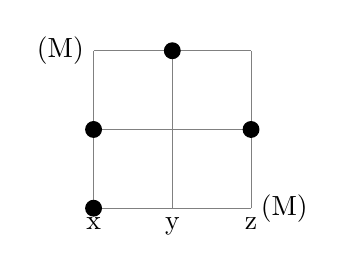
\begin{tikzpicture}
\draw[help lines] (0,0) grid (2,2);
\node [below] at (0,0) {x}; \node [below] at (1,0) {y}; \node [below] at (2,0) {z};
\node [left] at (0,2) {(M)};\node [right] at (2,0) {(M)};
\draw[fill] (0,0) circle [radius=0.1];
\draw[fill] (0,1) circle [radius=0.1];
\draw[fill] (1,2) circle [radius=0.1];
\draw[fill] (2,1) circle [radius=0.1];

\end{tikzpicture}
\subparagraph{Reflexivität} Die Diagonale $I_M = \{(x,x) \vert x\in M\}$ gehört zu $T$ ($I_M$ heißt auch Identitätsrelation, diese Relation ist eine spezielle Funktion)
\subparagraph{Symmetrie}T ist spiegelsymmetrisch zu $I_M$

\paragraph{Alternative Schreibweisen}
Es sei $T \subseteq M_1 \times M_2$ eine binäre Relation. An Stelle $(x,y) \in T$ kann man auch schreiben:
\begin{enumerate}
\item $x \; T \; y$
(x steht in Relation T zu y), für viele Relationen gibt es spezielle Zeichen z.B. $x < y$, $g || h$.
\item Aussagenfunktion (vlg. Prädikatenlogik) $T(x,y)$ (auch mehrstellig möglich) 
\end{enumerate}

\paragraph{Operationen auf Relationen}

Da Relationen spezielle Mengen sind, gibt es die Operation $\cap \cup$ usw. auch hier. Weitere für Relationen typische Operationen vgl. Definition 9-11.

\subparagraph{Definition 9} Es sei $T$ eine Relation in $U\times V$\\
Die Menge
\[proj_1 (T) = \{ x \in U | \exists y\in V \quad (x,y) \in T\}\]
heißt Projektion von T auf U. (1. Faktor des Produkts)\\
Analog ist
\[ proj_2 (T) = \{ y \in V | \exists x \in U \quad (x,y) \in T\}\]
die Projektion von $T$ auf den 2. Faktor ($V$) des Produkts $U\times V$.

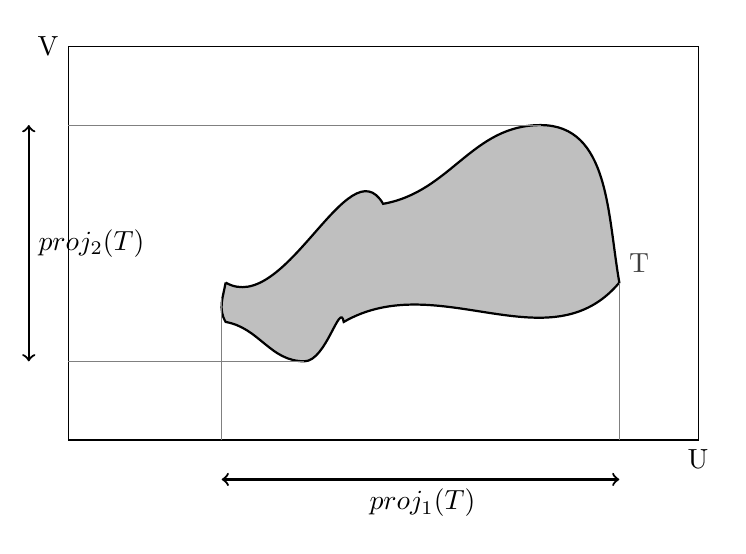
\begin{tikzpicture}


\draw [fill=lightgray,thick](2,2) to [out=-30,in=120] (4,3) to [out=10,in=180] (6,4) to [out=0,in=100] (7,2) to [out=230,in=30] (3.5,1.5) to [out=100,in=0] (3,1) to [out=180,in=-10] (2,1.5) to [out=120,in=260] (2,2);

\draw (0,0) rectangle (8,5);

\node [left] at (0,5) {V}; \node [above right,darkgray] at (7,2) {T}; \node [below] at (8,0) {U};

\draw [help lines] (0,1) -- (3,1); 
\draw [<->,thick] (-0.5,1) -- (-0.5,4); \node [right] at (-0.5,2.5) {$proj_2(T)$};
\draw [help lines] (0,4) -- (6,4);

\draw [help lines] (1.95,0) -- (1.95,1.8);
\draw [<->,thick] (1.95,-0.5) -- (7,-0.5); \node [below] at (4.5,-0.5) {$proj_1(T)$};
\draw [help lines] (7,0) -- (7,2);


\end{tikzpicture}

\subparagraph{Definition 10} Es sei $T \subseteq M_1 \times M_2$ eine binäre Relation\\
Die Relation
\[ T^{-1} := \{ (y,x) | (x,y) \in T\} \subseteq M_2\times M_1\]
heißt inverse Relation zu $T$ (kurz Inverse).

\paragraph{Definition 11} Es seien $T_1 \subseteq M_1 \times M_2$ und $T_2 \subseteq M_2 \times M_3$ binäre Relationen. Als Komposition (oder Verkettung) $T_1 \circ T_2$ wird folgende Relation
\[T_1 \circ T_2 :=\{(x,z)\in M_1 \times M_3 | \exists y \in M_2 \quad ((x,y) \in T_1 \wedge (y,z) \in T_2 )\}\]
in $M_1 \times M_3$ bezeichnet.

\subparagraph{Diskussion}
Wichtige Eigenschaft der Komposition $\circ$:
Die Operation $\circ$ ist assoziativ, d.h.  sei $T_1 \subseteq A \times B, T_2 \subseteq B \times C$ und $T_3 \subseteq C \times D$, dann gilt $(T_1 \circ T_2)\circ T_3 = T_1 \circ (T_2 \circ T_3) =:  T_1 \circ T_2 \circ T_3 \subseteq A \times D$


\subparagraph{Definition 12}
Es sei $T$ eine Relation in $M \times M$ (auf M). Als transitive Hülle $T^+$ von $T$ bezeichnet man die kleinste Relation die $T$ enthält und transitiv ist.

Satz 1
Es gilt 
\[T^+ = T \cup (T \circ T) \cup (T \circ T \circ T) \cup ...\]

\subparagraph{Bemerkung}
Bezeichnung für $\underbrace{T \circ T \circ ... \circ T}_{n-mal}$ auch $T^n$.

Achtung nicht zu verwechseln mit dem Mengenprodukt $T \times T\times ...\times T$ bzw. bei Funktion mit der n-ten Potenz $f^n$ Damit ist
\begin{equation*}
T^+ = \bigcup\limits_{g=1}^\infty T^j
\end{equation*}

Beweis:
\begin{enumerate}
\item $T^+$ ist transitiv, dann sei $(x,y) \in T^+ \wedge (y,z) \in T^+$, dann existiert natürliche Zahlen $j_1,j_2 \geq 1$ mit $(x,y) \in T^{j_1}$ und $(y,z) \in T^{j_2}$, d.h. y wird in $j_1$ Schritten von $x$ aus erreicht und $z$ in $j_2$ Schritten von $y$ aus.
Also wird $z$ in $j_1 + j_2$ Schritten von $x$ aus erreicht, d.h.:
$(x,z) \in T_{j_1 + j_2} \Rightarrow (x,z) \in T^+$.
\item Es sei $T \subseteq S$ für eine transitive Relation $S \Rightarrow T\circ T \subseteq S \circ S \subseteq S$ und für beliebiges $j \geq z$ \quad 
$ T^j \subseteq S^j \subseteq S$ und damit $T^+ = \bigcup\limits_{g=1}^{\infty} T^j \subseteq S$, d.h. $T^+$ ist tatsächlich die kleinste transitive Relation, die $T$ enthält.
\end{enumerate}
\subparagraph{Diskussion}
\begin{enumerate}
\item Analog zur transitiven Hülle einer RElation $T$ in $M \times M$ (auf M) werden die reflexive bzw. die symmetrische Hülle als die jeweils kleinsten Relationen, die T enthalten und die entsprechende Eigenschaft besitzen, erklärt. Die Ermittlung gestattet sich etwas einfacher als bei der transitiven Hülle.

Reflexive Hülle von $T$:
\[T\cup I_M\]
dabei $I_M =\{ (x,x) | x \in M\}$ \dots Identitätsrelation.

Symmetrische Hülle von $T$:
$T \cup T^{-1}$
\item Von Bedeutung ist auch die reflexiv-transitive Hülle von $T: \quad T^* := T^+ \cup I_M$
(dabei $T^*$ transitive Hülle)
\end{enumerate}

\subparagraph{Beispiel 8} Gegeben sei die Menge $M =\{ a,b,c,d,e,f\}$ sowie die Relation\\* $T=\{(a,b,),(b,c),(c,e),(b,d),(d,e),(e,f)\}$
\begin{enumerate}
\item Transitive Hülle

Zur Ermittlung der Elemente eines Komposition $S \circ T$: Für jedes Element $(x,y)\in S$ alle Fortsetzungen $(y,z_i)\in T$ suchen $\curvearrowright (x,z_i)$ als Element von $S \circ T$ notieren, falls noch nicht vorhanden.

Also $T\circ T: (a,b)$ Fortsetzung $(b,c),(b,d) \curvearrowright (a,c),(a,d)$ \\* $(b,c)$ Fortsetzung $(c,e) \curvearrowright (b,c)$\\
$\curvearrowright T \circ T = T^2 = \{(b,c,),(b,d),(c,e),(c,f)$
$\curvearrowright T^3 = T\circ T^2=\{(a,e),(b,f)\}$
$\curvearrowright T^4 = T\circ T^3 =\{ (a,f)\}$
$\curvearrowright T^5 = T\circ T^4 = \varnothing \curvearrowright T^+ = T\cup T^2 \cup T^3 \cup T^4$

\item Reflexive Hülle: $T\cup \{(a,a),(b,b),(c,c),(d,d),(e,e),(f,f)\}$
\item Symmetrische Hülle: $T\cup T^{-1} = T \cup \{(b,a),(c,b),...\}$
\end{enumerate}

Zur Überprüfung der Eigenschaften aus Definition 8 ist folgender Satz nützlich:
\subparagraph{Satz 2} Es sei $T \subseteq M \times M$ eine binäre Relation. Dann gilt:
\begin{enumerate}
\item $T$ ist reflexiv $\Leftrightarrow I_M \subseteq T$ ($I_M$ \dots Identitätsrelation)
\item $T$ ist symmetrisch $\Leftrightarrow T^{-1} \subseteq T ( \Leftrightarrow T^{-1} = T)$
\item $T$ ist antisymmetrisch $\Leftrightarrow T \cap T^{-1} \subseteq I_M$ \label{c)}
\item $T$ ist asymmetrisch $\Leftrightarrow T \cap T^{-1} = \varnothing$
\item $T$ ist transitiv $\Leftrightarrow T\circ T \subseteq T$
\end{enumerate}

\subparagraph{Diskussion} Aus c) und d) ergibt sich
\begin{quote}
T asymmetrisch $\Rightarrow$ T antisymmetrisch
\end{quote}
(da $\varnothing$ Teilmenge jeder Menge ist, auch von $I_M$)

\paragraph{Äquivalenzrelationen}
\subparagraph{Definition 13}
Eine Relation $T \subseteq M \times M$ heißt Äquivalenzrelation, wenn sie reflexiv, symmetrisch und transitiv ist:

Diskussion:
\begin{enumerate}
\item Durch eine Äquivalenzrelation wird $M$ vollständig in paarweise elementfremde (disjunkte) Äquivalenzklassen zerlegt. Die Menge aller Äquivalenzklassen von $M$ bezüglich $T$ heißt Quotientenmenge $M/T$.

Aufgrund der 3 Eigenschaften aus Definition 13 enthält eine Äquivalenzklasse alle Elemente die untereinander erreichbar sind und nur diese.

\item Äquivalenzklassen enthalten alle Elemente die bezüglich einer bestimmten Eigenschaft nicht unterscheidbar sind (= äquivalent), z.B. Beispiel 4b mit $M=P$ (Menge von Personen), Äquivalent $G \subseteq P \times P$ mit $\{ (x,y) |$ x u. haben gleiches Geburtsjahr\}, Äquivalenzklassen sind die Jahrgänge.

\item Anstelle der Schreibweisen $(x,y,)\in T, \quad \times T y$ oder $T(x,y)$ verwendet man bei beliebigen Äquivalenzklassen auch $x \sim y$. Bei vielen speziellen Äquivalenzrelationen spezielle Symbole, vlg. Beispiel 9.

\subparagraph{Beispiel 9}\label{Bsp9}
\begin{enumerate}
\item $M$ sei eine beliebige Menge $T_1 = I_M = \{ (x,y) \in M \times M | x=y\}$ (Identitätsrelation) ist eine Äquivalenzrelation. Äquivalenz heißt hier gleich!
Äquivalenzklassen sind sämtliche einelementige Teilmengen $\{x\} , x \in M$. $T_1$ liefert die feinste Zerlegung von M, die möglich ist. Die gröbste "`Zerlegung"' liefert die Relation $T_2 = M \times M$, die trivialerweise eine Äquivalenzrelation ist (mit nur einer Äquivalenzklasse M). Für die Anwendungen wichtig: Relationen, die eine echte Zerlegung liefern.

\item $M= \mathbb{Z}$ (ganze Zahlen), $m \in \mathbb{N}^*, T \subseteq \mathbb{Z} \times \mathbb{Z}$ mit
\begin {enumerate}
\item $(x,y) \in T :=$ "`x und y lassen bei Division den gleichen Rest"'
\item Bezeichnung $x \equiv y (\mod{m})$ x kongruent y (modulo m)
z.B. $29 \equiv 8 (\mod{7})$
\item $T$ ist eine Äquivlenzrelation auf $\mathbb{Z}$, Äquivalenzklassen: Restklassen (modulo M).
\end{enumerate}

\item $M$\dots Menge aller Geraden einer Ebene, $T\subseteq M \times M$ mit
$(x,y) \in T :=$ "`x ist parallel zu y"'.
Bezeichnung $x\parallel y$, T ist Äquivalenzrelation auf $M$.

\end{enumerate}
\end{enumerate}

\paragraph{Ordnungsrelation}%1.2.3.4.
\subparagraph{Definition 14}
\begin{enumerate}
\item Eine Relation $T \subseteq M \times M$ heißt Ordnungsrelation auf $M$, wenn sie reflexiv, antisymmetrisch und transitiv ist.
\item Eine Ordnungsrelation heißt vollständig (oder linear), wenn für alle $x,y \in M$ gilt $(x,y) \in T \vee (y,x) \in T$

\end{enumerate}

\subparagraph{Definition 15} Eine Relation $T \subseteq M \times M$ heißt strikte Ordnungsrelation, wenn sie asymmetrisch und transitiv ist. Eine strikte Ordnung heißt vollständig (linear), wenn für alle $x,y \in M$ mit $x\neq y$ gilt: $(x,y) \in T \wedge (y,x) \in T$

\subparagraph{Beispiel 10}
\begin{enumerate}
\item $M = \mathbb{R}, T \subseteq \mathbb{R} \times \mathbb{R}$ mit $(x,y)\in T := x \leq y$ ist eine vollständige Ordnungsrelation auf $\mathbb{R}$
\item Die Relation "`$<$"' ist eine vollständige, strikte Ordnung auf $\mathbb{R}$.
\item $E$ sei die Menge, $M$ sei die Menge aller Teilmengen von $E$, die sogenannte Potenzmenge $M = \mathcal P(E) \quad T \subseteq M \times M$ mit $(A,B) \in T := A\subseteq B$ ist eine Ordnungsrelation $\mathcal P(E)$ (Inklusion)

\end{enumerate}

Diskussion:
\begin{enumerate}
\item In der Literatur wird manchmal eine Relation im Sinne der Definition 14 als Halbordnung und nur eine vollständige Ordnung als Ordnungsrelation bezeichnet.
\item Zu jeder Ordnung $T_1$ (auf $M$) gehört eine strikte Ordnung $T_2$ und umgekehrt.
\[ T_2 = T_1 \backslash I_M \quad \text{bzw.} \quad T_1 = T_2 \cup I_M\]
($T_1$ ist die reflexive Hülle von $T_2$), z.B. $(\leq ,<)$ oder $(\subseteq , \subset )$
\item Die Symbole $\leq$ bzw. $<$ können anstelle der Paarschreibweise auch bei beliebigen Ordnungen verwendet werden, falls keine anderen Symbole vorhanden.

\end{enumerate}

\subparagraph{Definition 16} T sei eine Ordnungsrelation auf einer Menge $M$. Weiter sei $A$ eine Teilmenge von $M$.
\begin{enumerate}
\item Ein Element $a \in M$ heißt obere Schranken von $A$, wenn $\forall x \in A \quad x \leq a$, d.h. $(x,a) \in T$ vgl. Diskussion 3.
\item Es sei $B$ die Menge aller oberen Schranken von $A$ ($B\neq \varnothing$). Falls es eine kleinste obere Schranke $s$ von A gibt, d.h.
$\exists s \in B \forall b \in B \quad s\leq b$, so heißt $s$ das Supremum von $A$, $s = \sup{A}$
\item Gilt $s\in A$, so heißt $s$ das Maximum von $A$, $s=\max{A} = \sup{A}$
\item Ein Element $M \in A$ heißt maximal, wenn es kein größeres Element in $A$ gibt, d.h. $\forall x\in A \quad ( m \leq x \Rightarrow m=x)$

\end{enumerate}

Diskussion:
\begin{enumerate}
\item Die Begriffe aus Definition 16, lassen sich auf strikte Ordnungen $S$ übertragen, indem anstelle von $S$ die reflexive Hülle $S \cup I_M$ verwendet wird.
\item Bei Ordnugnsrelationen $T$ (auch strikten) auf endlichen Mengen $M$, kann ein vereinfachter Graph, das sogenannte \textsc{Hasse} -Diagramm betrachtet werden:
$a \rightarrow b (a\neq b)$ bedeutet $(a,b) \in T$ und es gibt kein Zwischenglied $c \neq a$ und $c \neq b$ mit $(a,c) \in T \wedge (c,b) \in T$, ($b$ ist unmittelbar Nachfolger von $a$ bzw. $a$ ist unmittelbar Vorgänger von $b$)

Diesem Diagramm entspricht eine Teilrelation $U \subseteq T$, deren transitiv-reflexive Hülle (bzw. transitive Hülle bei strikten Ordnungen) die Relation $T$ ist.
\item Veranschaulichung von Definition 16 mit einem \textsc{Hasse} Diagramm einer nicht-vollständigen Ordnung (nicht linear)

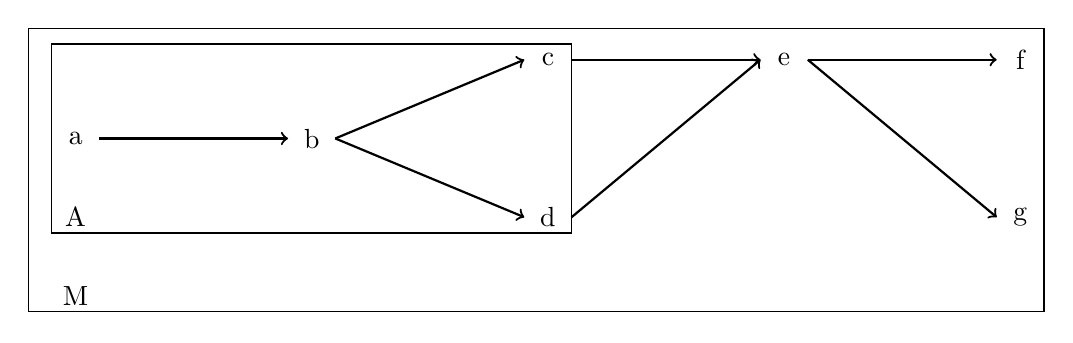
\begin{tikzpicture}[xscale=3]
%\draw [help lines] (0,0) grid (4,3);
\node at (2,3) {c}; \draw [->,thick] (2.1,3) -- (2.9,3); \node at (3,3) {e}; \draw [->,thick] (3.1,3) -- (3.9,3); \draw [->,thick] (3.1,3) -- (3.9,1); \node at (4,3) {f};
\node at (0,2) {a}; \draw [->,thick] (0.1,2) -- (0.9,2); \node at (1,2) {b}; \draw [->,thick] (1.1,2) -- (1.9,3); \draw [->,thick] (1.1,2) -- (1.9,1);
\draw (-0.1,0.8) rectangle (2.1,3.2);  \node at (0,1) {A}; \node at (2,1) {d}; \draw [->,thick] (2.1,1) -- (2.9,3); \node at (4,1) {g};
\draw (-0.2,-0.2) rectangle (4.1,3.4); \node at (0,0) {M};



\end{tikzpicture}

obere Schranken von $A : e,f,g$
kleinste obere Schranke $= \sup{A} = e$
$\max{A}$ existiert nicht, da $e \notin A$

maximale Elemente von $A: c,d$ (es gibt in A keine größeren)
\item Bei nicht linearen Ordnungen müssen obere Schranken, Supremum und Maximum nicht existieren, es kann mehrere maximale Elemente geben (von $A \subset M$) Bei linearen Ordnungen auf endlichen Mengen gibt genau ein maximales Element $= \max{A} = \sup{A}$

\item Analog zur Definition 16 werden die Begriffe untere Schranke $a$ von $A \quad (\forall x \in A \quad a\leq x)$, größte untere Schranke (=Infimum) $s$ von $A$ $(B \neq \varnothing$ \dots Menge der unteren Schranken, $\exists s \in B \quad \forall a \in B \quad a \leq s)$, Minimum von $A (\min{A} = \inf{A}=s \quad \text{falls} \quad  s \in A)$ und minimales Element $m$ von $A (\forall x \in A \quad ( x \leq m \Rightarrow x=m)$ definiert.
\end{enumerate}
\subparagraph{Beispiel 11:} Eine bestimme Arbeitsaufgabe besteht aus mehreren Arbeitsgängen. Es sei $A=\{1,2,3,4,5,6\}$ die Menge der Arbeitsgänge. Die Arbeitsgänge $\{2,3,5\}=:S$ werden von einer Subfirma durchgeführt. Für die Reihenfolge gilt: 1 muss vor 2, 2 vor 3 und vor 5, 3 vor 4, sowie 5 vor 6 durchgeführt werden.
\begin{enumerate}
\item Man beschreibe diese Forderungen durch eine Relation $U \subseteq A \times A$ und stelle sie graphisch dar. \label{AufgA}
\item Man ermittle die transitive Hülle $U^+$ von $U$.\label{AufgB}
\item Man gebe (falls vorhanden) obere Schranken, Supremum, Maximum, maximimale \label{AufgC} Elemente, sowie untere Schranken, Infimum, Minimum und minimale Elemente von $S$ an.
\end{enumerate}

Lösung: 
\begin{enumerate}
\item $U=\{(1,2),(2,3),(2,5),(3,4),(5,6)\}$

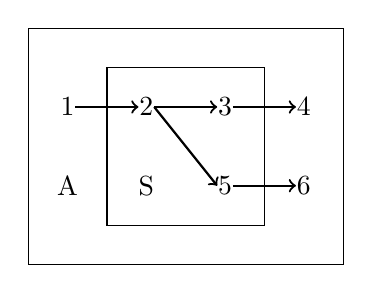
\begin{tikzpicture}
\node at (0,0) {1}; \draw [->,thick] (0.1,0) -- (0.9,0); \node at (1,0) {2}; \draw [->,thick] (1.1,0) -- (1.9,-1); \draw [->,thick] (1.1,0) -- (1.9,0); \node at (2,0) {3}; \draw [->,thick] (2.1,0) -- (2.9,0); \node at (3,0) {4};
\node at (2,-1) {5}; \draw [->,thick] (2.1,-1) -- (2.9,-1); \node at (3,-1) {6};

\draw (0.5,-1.5) rectangle (2.5,0.5); \node at (1,-1) {S};
\draw (-0.5,-2) rectangle (3.5,1); \node at (0,-1) {A};

\end{tikzpicture}

\item $U \circ U = \{(1,3),(1,5),(2,4),(2,6)\}\\
U^3 = U \circ U^2 = \{(1,4),(1,6)\}\\
U^4 = U \circ U^3 = \varnothing \\
\implies U^+ = U \cup U^2 \cup U^3 = ...$

$U^+$ ist asymmetrisch und transitiv, also strikte Ordnung (Skizze \dots \textsc{Hasse} Diagramm

\item
\begin{itemize}
\item $S$ hat keine oberen Schranken, kein Supremum, kein Maximum; aber maximale Elemente: $3,5$
\item untere Schranken $1,2,  \inf{S} = \min{S} = 2$ (=einziges minimales Element)
\end{itemize}
\end{enumerate}

\paragraph{Funktionen}
\subparagraph{Definition 17:} Eine Relation $f\subseteq \mathcal{X} \times \mathcal{Y}$ heißt Funktion (Abbildung) von $\mathcal{X}$ in $\mathcal{Y}$, wenn sie linksvollständig und rechtseindeutig ist.

Diskussion:
\begin{enumerate}
\item Gemäß Definition 7 \ref{def7a} und \ref{def7c} bedeutet linksvollständig und rechtseindeutig, dass zu jedem $x \in \mathcal{X}$ genau ein $y \in \mathcal{Y}$ mit $(x,y) \in f$ existiert, also eindeutige Zuordnung
\[x \rightarrow y =: f(x)\]

Schreibweise
\[ f| \mathcal{X} \rightarrow \mathcal{Y}\]

$y = f(x)$ heißt auch Bild von $x$,
$x$ heißt ein Urbild von $y$ (muss nicht eindeutig sein)
\item $\mathcal{X} =: Db(f)$\dots Definitionsbereich\\
$Wb(f):=\{y\in \mathcal{Y} | \exists x \in \mathcal{X} \quad (x,y) \in f\}$\\
$\subseteq \mathcal{Y}$\dots Wertebereich\\
Schreibweise auch $f(\mathcal{X}):= Wb(f)$
\end{enumerate}

\subparagraph{Definition 18}
\begin{enumerate}
\item Eine Abbildung $f$ heißt surjektiv (auch Abbildung auf $\mathcal{Y}$, wenn $Wb(f)=\mathcal{Y}$
\item Eine Funktion $f$ heißt injektiv (auch umkehrbar, eindeutig oder eineindeutig), wenn es zu jedem $y \in Wb(f)$ genau ein $x \in Db(f)$ existiert mit $(x,y) \in f:$

\[\underbrace{y}_{\in Wb(f)} \longrightarrow \underbrace{x}_{\in Db(f)} =: f^{-1}(y)\]
Die dadurch erklärte Abbildung $f^{-1}| Wb(f) \rightarrow Db(f)$ heißt Umkehrfunktion von $f$, vgl. auch Kapitel 1.4.
\item Eine injektive und surjektive Abbildung heißt bijektiv.
\item Gebräuchlich sind auch die Begriffe Surjektion, Injektion und Bijektion
\end{enumerate}

\subparagraph{Beispiel 12:} Gegeben seien die Mengen $\mathcal{X} = \{ a,b,c\}$ und $\mathcal{Y} = \{1,2,3,4\}$, sowie folgende Relationen in $\mathcal{X} \times \mathcal{Y}:$

\begin{enumerate}
\item $T_1:$\\*
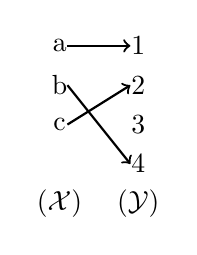
\begin{tikzpicture}[yscale=0.5]
\node at (0,0) {a}; \draw [->,thick] (0.1,0) -- (0.9,0); \node at (1,0) {1};
\node at (0,-1) {b}; \draw [->,thick] (0.1,-1) -- (0.9,-3); \node at (1,-1) {2};
\node at (0,-2) {c}; \draw [->,thick] (0.1,-2) -- (0.9,-1); \node at (1,-2) {3};
\node at (1,-3) {4};
\node at (0,-4) {$(\mathcal{X})$}; \node at (1,-4) {$(\mathcal{Y})$};


\end{tikzpicture}

$T_1$ ist eine Funktion (da linksvollständig und rechtseindeutig), Funktion $f = T_1 :\: f|\mathcal{X} \rightarrow \mathcal{Y}$, diese ist injektiv, $Db(f)=\mathcal{X}, Wb(f) = \{1,2,4\}=:W$

Die Abbildung $f|\mathcal{X} \rightarrow W$ ist auch surjektiv, also bijektiv.
Als Relationen sind $f|\mathcal{X} \rightarrow \mathcal{Y}$ und $f|\mathcal{X} \rightarrow W$ nicht zu unterscheiden, aber als Funktionen.

\item $T_2:$\\*
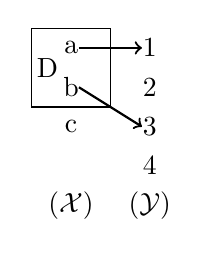
\begin{tikzpicture}[yscale=0.5]
\node at (0,0) {a}; \draw [->,thick] (0.1,0) -- (0.9,0); \node at (1,0) {1};
\node at (0,-1) {b}; \draw [->,thick] (0.1,-1) -- (0.9,-2); \node at (1,-1) {2};
\node at (0,-2) {c}; \node at (1,-2) {3};
\node at (1,-3) {4};
\node at (0,-4) {$(\mathcal{X})$}; \node at (1,-4) {$(\mathcal{Y})$};

\draw (-0.5,0.5) rectangle (0.5,-1.5); \node at (-0.3,-0.5) {D};

\end{tikzpicture}

$T_2$ ist keine Funktion, da nicht linksvollständig. Betrachtetman $D:=\{a,b\}$, so wird durch $T_2$ eine Funktion $f|D\rightarrow \mathcal{Y}$ beschrieben, diese ist injektiv und kann mit $W:= f(D) =Wb(f)=\{1,3\}$ zu einer bijektiven Abbildung $f|D\rightarrow W$ umgewandelt werden.

\item $T_3:$\\*
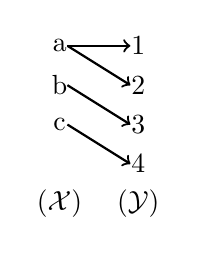
\begin{tikzpicture}[yscale=0.5]
\node at (0,0) {a}; \draw [->,thick] (0.1,0) -- (0.9,0); \draw [->,thick] (0.1,0) -- (0.9,-1); \node at (1,0) {1};
\node at (0,-1) {b}; \draw [->,thick] (0.1,-1) -- (0.9,-2); \node at (1,-1) {2};
\node at (0,-2) {c}; \draw [->,thick] (0.1,-2) -- (0.9,-3); \node at (1,-2) {3};
\node at (1,-3) {4};
\node at (0,-4) {$(\mathcal{X})$}; \node at (1,-4) {$(\mathcal{Y})$};


\end{tikzpicture}


$T_3$ ist keine Funktion, da nicht rechtseindeutig.

\end{enumerate}

\subparagraph{Beispiel 13:}
\begin{enumerate}
\item $f|[0,\infty ) \rightarrow \mathbb{R}$ mit $x\rightarrow y = f(x) = \sqrt{x}$ ist eine Funktion einer reellen Veränderlichen (injektiv, $Db(f)=[0,\infty )$

\item $f| \mathbb{R} \times \mathbb{R} \rightarrow \mathbb{R}$ mit $z=f(x,y)=x^2 +y^2$\\
$(x,y) \rightarrow f(x,y) = x^2 +y^2 =:z$
Funktion zweier reeller Veränderlichen

\item $f|\mathbb{N} \rightarrow \mathbb{R}$ mit $n \rightarrow f(n) = \frac{n}{n+1}$ \dots reelle Zahlenfolge $f(0) = 0, f(1) = \frac{1}{2}, f(2) = \frac{2}{3}, ...$
Bezeichnung meist mit Index $a_n := f(n) \curvearrowright$ Folge $(a_n)_{n \in \mathbb{N}}$
\end{enumerate}


\subparagraph{Definition 19} Es seien $g|\mathcal{X} \rightarrow U$ mit $x \rightarrow u = g(x)$ und $f|U \rightarrow \mathcal{Y}$ mit $u \rightarrow y = f(u)$ zwei Abbildungen. Dann stellt die Zuordnung $x \rightarrow y = f(\underbrace{g(x)}_{u})$ eine Abbildung von $\mathcal{X}$ in $\mathcal{Y}$ dar, eine sogenannte mittelbare Funktion (Komposition/Verkettung).

Bezeichnung: $g \circ f | \mathcal{X} \rightarrow \mathcal{Y}$ mit $y=(g\circ f)(x) = f(g(x))$

Diskussion: 
\begin{enumerate}
\item 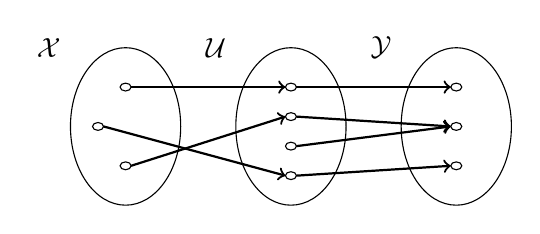
\begin{tikzpicture}[yscale=0.5, xscale=0.7]
%\draw (0,0) grid (2,2);
\node [left] at (-1,2) {$\mathcal{X}$};
\draw (0,0) circle [x radius=1, y radius=2];
\draw (0,1) circle [radius=0.1]; \draw (-0.5,0) circle [radius=0.1]; \draw (0,-1) circle [radius=0.1]; 

\draw [->,thick] (0.1,1) -- (2.9,1);
\draw [->,thick] (-0.4,0) -- (2.9,-1.25);
\draw [->,thick] (0.1,-1) -- (2.9,0.25);

\node [left] at (2,2) {$\mathcal{U}$};
\draw (3,0) circle [x radius=1, y radius=2];
\draw (3,1) circle [radius=0.1]; \draw (3,0.25) circle [radius=0.1]; \draw (3,-0.5) circle [radius=0.1]; \draw (3,-1.25) circle [radius=0.1]; 

\draw [->,thick] (3.1,1) -- (5.9,1);
\draw [->,thick] (3.1,0.25) -- (5.9,0);
\draw [->,thick] (3.1,-0.5) -- (5.9,0);
\draw [->,thick] (3.1,-1.25) -- (5.9,-1);

\node [left] at (5,2) {$\mathcal{Y}$};
\draw (6,0) circle [x radius=1, y radius=2];
\draw (6,1) circle [radius=0.1]; \draw (6,0) circle [radius=0.1]; \draw (6,-1) circle [radius=0.1]; 

\end{tikzpicture}
\begin{align*}
        x \rightarrow u=g(x) &| u\rightarrow y =f(u)=f(g(x))\\
\text{Paarschreibweise} (x,u) \in g &| (u,y) \in f \curvearrowright (x,y) \in g \circ f 
\end{align*}

\item $g$ wird zuerst angewendet, dann $f$; wie bei beliebigen Relationen, also Schreibweise $g \circ f$

\item In der Literatur findet man leider oft die Schreibweise $f \circ g$, offenbar angelehnt an die Schreibweise $f(g(x))$. Die Reihenfolge ist aber von innen nach außen, erst $g$, dann $f$.

\Large{Bei allen späteren Anwendungen von mittelbaren Funktionen (Vorlesungen,Literatur) die Schreibweise überprüfen. Im Zweifelsfall stets die immer eindeutige Schreibweise $f(g(x))$ ohne Verwendung von "`$\circ$"' benutzen!}
\end{enumerate}

\subparagraph{Satz 3} Es sei $f|\mathcal{X} \rightarrow \mathcal{Y}$ eine Bijektion, d.h. es existiert die Umkehrfunktion $f^{-1} | \mathcal{Y} \rightarrow \mathcal{X}$. 
Weiter bezeichne für eine beliebige Menge $A$ die Schreibweise $i_A$ die identische Abbildung (Identitätsrelation, d.h. $i_A | A \rightarrow A$ und $i_A(x)=x \, (x \in A)$.

Es gilt dann:
\[f\circ f^{-1} = i_{\mathcal{X}}, \text{d.h.} (f \circ f^{-1})(x) = f^{-1}(f(x))=x \quad (\forall x \in \mathcal{X} )\]
\[f^{-1} \circ f = i_{\mathcal{Y}}, \text{d.h.} (f^{-1} \circ f)(y) = f(f^{-1}(y))=y \quad (\forall y \in \mathcal{Y} )\]
(Funktion und Umkehrfunktion nacheinander angewandt "`heben sich auf"')

Beweis: ÜA 1.31

\subparagraph{Satz 4} Es seien $g|\mathcal{X} \rightarrow U$ und $h|U\rightarrow \mathcal{Y}$ zwei Bijektionen. Dann ist die Komposition $f:= g\circ h | \mathcal{X} \rightarrow \mathcal{Y}$ ebenfalls eine Bijektion und es gilt:
\[f^{-1}=(g\circ h)^{-1} = h^{-1} \circ g^{-1} \]

Zum Beweis: $x \rightarrow u=g(x) \rightarrow y=h(u) = h(g(x)) = (g \circ h)(x)$\\
Umkehrung: $y\rightarrow u = h^{-1}(y) \rightarrow x=g^{-1}(u) =g^{-1}(h^{-1}(y)) = (h^{-1} \circ g^{-1})(y)$\\
Mehr zu Imkehrfunktionen reeller Funktionen im Kapitel 1.4..

\subsubsection{Gleichmächtigkeit,Kardinalzahlen}
$E$ sei eine (hinreichend umfassende) Grundmenge, die alle für eine mathematische Theorie relevanten Objekte (Zahlen,Funktionen usw.) enthält.

$M$ sei die Potenzmenge von $E$, d.h. $M = \mathcal{P} (E)$

\subparagraph{Definition 20} Zwei Mengen $A$ und $B \quad (A \subseteq E, B\subseteq E \text{bzw.} A \in M, B\in M)$ heißen gleichmächtig.
(Bezeichnung $(A \sim B)$, wenn eine bijektive Abbildung von $A$ auf $B$ (und damit auch von $B$ auf $A$ bzw. zwischen $A$ und $B$) existiert.

Diskussion:

\begin{enumerate}
\item Offensichtlich ist die Relation $T \subseteq M \times M$ mit $(A,B) \in T := A \sim B$ eine Äquivalenzrelation auf $M$.

\item Äquivalenzklassen sind MEngen gleichmächtiger Teilmengen von $E$. Diese Äquivalenzklassen nennt man Kardinalzahlen.
\item Bei endlichen Mengen bedeutet Gleichmächtigkeit: gleiche Anzahl von Elementen.

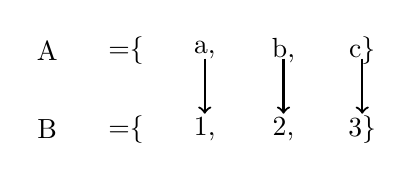
\begin{tikzpicture}

\node at (0,0) {A}; \node at (1,0) {=\{ }; \node at (2,0) {a,}; \node at (3,0) {b,};\node at (4,0) {c\}};

\draw [->,thick] (2,-0.1) -- (2,-0.8);\draw [->,thick] (3,-0.1) -- (3,-0.8);\draw [->,thick] (4,-0.1) -- (4,-0.8);

\node at (0,-1) {B}; \node at (1,-1) {=\{ }; \node at (2,-1) {1,}; \node at (3,-1) {2,};\node at (4,-1) {3\}};

\end{tikzpicture} (bijektive Abbildung)

Bezeichnung: $card\,A = \lvert A \rvert = 3 = \lvert B \rvert$
Natürliche Zahlen sind die Kardinalzahlen endlicher Mengen.

\item Die Anschauung versagt bei unendlichen Mengen.


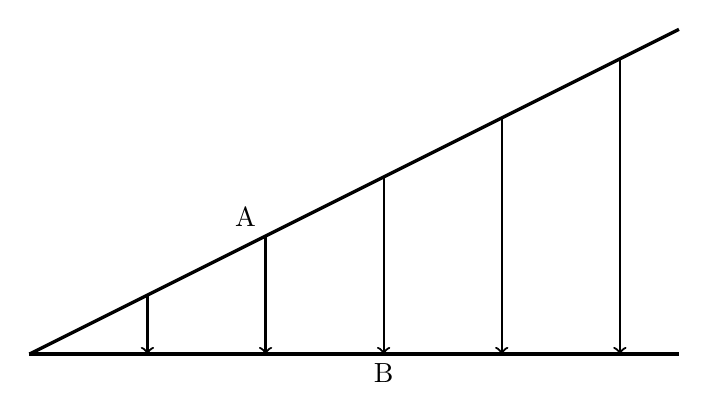
\begin{tikzpicture}[xscale=1.5,yscale=0.75]
%\draw (0,0) grid (5,5);

\node [above left] at (2,2) {A};
\draw [very thick] (0,0) -- (5.5,5.5);

\draw [->,thick] (1,1) -- (1,0); \draw [->,thick] (2,2) -- (2,0); \draw [->,thick] (3,3) -- (3,0); \draw [->,thick] (4,4) -- (4,0); \draw [->,thick] (5,5) -- (5,0); 

\node [below] at (3,0) {B};
\draw [very thick] (0,0) -- (5.5,0);
\end{tikzpicture}

Die Strecken $A$ und $B$ sind gleichmächtig, obwohl A länger als B ist.

\end{enumerate}


\subparagraph{Definition 21} Eine Menge heißt abzählbar unendlich, wenn sie mit der Menge $\mathbb{N} = \{0,1,2,3,...\}$ der natürlichen Zahlen gleichmächtig ist.

Diskussion:
\begin{enumerate}
\item $M$ ist abzählbar unendlich heißt, es existiert eine Zählvorschrift, bei der jedes Element von $M$ nach endlichen vielen Schritten erreicht wird.
\item Die Menge $\mathbb{Z}$ der  ganzen Zahlen ist abzählbar unendlich. 
Anordnung nach wachsenden Betrag: $\mathbb{Z}=\{0,-1,1,-2,2,-3,3,...\}$
\item $\mathbb{Q}^+$ \dots Menge der positiven rationalen Zahlen.
%Todo Optional Foto vom 2013-11-04T16:20

$\mathbb{Q}^+ = \{ \frac{1}{1}, \frac{1}{2}, \frac{2}{1},\frac{1}{3},\xout{\frac{2}{2}},\frac{3}{1}, ...\}$

$\curvearrowright$ Analog zu $\mathbb{Z}$: Die Menge der rationalen Zahlen $\mathbb{Q}$ ist abzählbar unendlich.

\item Es gibt Mengen, die mächtiger als die Menge der natürlichen Zahlen sind: Überabzählbare Mengen.

$B$ heißt mächtiger als $A$, wenn es eine injektive Abbildung $f|A \rightarrow B$ gibt, aber keine bijektive Abbildung, Schreibweise $\lvert A \rvert < \lvert B \rvert$, 

\end{enumerate}

\subparagraph{Satz 5} Die Menge $M=\{ x \in \mathbb{R} |0 < x <1\} = (0;1)$ ist überabzählbar.

Beweis: (\textsc{Cantor}sches Diagonalverfahren): Indirekt, angenommen $M=(0;1)$ sei abzählbar unendlich, d.h. $M=\{ x_1,x_2,x_3,...\} $. Für die Zahlen $x_h$ wählen wir z.B. die eindeutige Darstellung als Dezimalbruch (9er Periode verwenden)\\
$ x_1 = 0,a_1^{(1)} a_2^{(1)} a_3^{(1)} ...$\\
$x_2 = 0,a_1^{(2)} a_2^{(2)} a_3^{(2)} ...$\\
$x_3 = 0,a_1^{(3)} a_2^{(3)} a_3^{(3)} ...$\\
\dots

Es sei $z=0,b_1 b_2 b_3 ...$
mit $b_k =\left\{ \begin{array}{rcl}
         1
         & \mbox{falls}
         & a_k^{(k)} \neq 1 \\ 
         2  
         & \mbox{falls} 
         & a_k^{(k)} = 1 \\
                \end{array}\right. (k=1,2,3,...)$

Damit unterscheiden sich $x_k$ und $z$ auf jedem Fall an der $h$-ten Stelle $\curvearrowright z \neq x_k (\forall k)$, $z$ ist also nicht in der Folge $x_1,x_2,x_3,...$ enthalten, also $z \notin M$. Andererseits gilt $0<z<1$, also $z \in (0;1)=M$ Widerspruch. q.e.d.

\subparagraph{Satz 6} Es sei $E$ eine nichtleere Menge. Dann ist die Potenzmenge $M=\mathcal{P}(E)$ mächtiger als E.

Beweis: 
\begin{enumerate}
\item Die Abbildung $f|E \rightarrow M$ mit $f(x)=\{x\},$ die jedem Element $x \in E$ die eindeutige Teilmenge $\{x\} \in M$ zuordnet ist injektiv.
\item Angenommen, es gäbe eine bijektive damit auch surjektive) Abbildung $g|E \rightarrow M$
Es sei $A=\{x \in E | x \notin g(x)\} \in M$
\end{enumerate}
($A$ ist Teilmenge von $E$). Da $g$ surjektiv ist, gibt es ein Element $a \in E$ mit $g(a) = A$

Fallunterscheidung:\\*
\begin{enumerate}
\item $a\notin A = g(a) \rightarrow a \in A$ (Widerspruch)
\item $a\in A =g(a) \rightarrow a \notin A$ (Widerspruch)
\end{enumerate}
Beide Fälle führen auf Widerspruch, es gibt also keine surjektive Abbildung, damit auch keine bijektive Abbildung von $E$ auf $\mathcal{P}(E).|$

Diskussion: Satz 6 zeigt, dass es unendlich viele unendliche Mächtigkeiten gibt. Zum Beispiel gibt $\lvert \mathbb{N} \rvert < \lvert \mathcal{P} (\mathbb{N}) \rvert < \lvert \mathcal{P} (\mathcal{P} ( \mathbb{N}))\rvert$ usw.

\subparagraph{Satz 7} Die Potenzmenge $\mathcal{P}(\mathbb{N})$ der Menge der natürlichen Zahlen ist gleichmächtig dem Intervall (0;1), also überabzählbar.

Beweis: s ÜA 1.38

\paragraph{Prinzip der vollständigen Induktion} Es sei $n_0 \in \mathbb{N}$.
Zu beweisen ist: "`Für alle natürlichen Zahlen $n\geq n_0$ gilt die Aussage $p(n)$"' Es sind also abzählbar unendlich viele Aussagen zu beweisen.

\subparagraph{Satz 8}
\begin{enumerate}
\item Es sei $p(n_0)$ wahr. (Induktionsanfang)
\item Für alle natürlichen Zahlen $n\geq n_0$ sei die Implikation $p(n) \rightarrow p(n+1)$ wahr (Induktionsschluss)
\end{enumerate}
Dann gilt: $p(n)$ ist für alle $n\geq n_0$ wahr.

Zum Beweis:
\begin{enumerate}
\item $\curvearrowright p(n_0)$ wahr
\item $p(n_0) \rightarrow p(n_0 + 1)$
\end{enumerate}
Prämisse wahr, Implikation wahr $\curvearrowright$ Konklusion $p(n_0 +1 )$ wahr usw.
%%

Beispiel 14: Zu beweisen ist 
\[ \sum\limits_{k=1}^{n} k^2 = \frac{n(n + 1)(2n + 1)}{6} \text{ für alle } n\in N^*\]
\begin{enumerate}
\item $p(1): 1^2 = \frac{1\cdot 2\cdot 3}{6}$ (wahr) Induktionsanfang
\item Es gelte $p(n): \sum\limits_{k=1}^{n} k^2 = \frac{n(n + 1)(2n + 1)}{6}$
\end{enumerate}
zu zeigen $p(n+1) : \sum\limits_{k=1}^{n+1} k^2 = \frac{(n+1)(n+2)(2n+3)}{6}$

Induktionsschluss: $p(n) \rightarrow p(n+1)$\\
$\sum\limits_{k=1}^{n+1} k^2 = \sum\limits_{k=1}^{n} k^2 + (n+1)^2$\\
$= \frac{n(n+1)(2n+1)}{6} + (n+1)^2$\\
$= \frac{n+1}{6} (n(2n +1) + 6(n+1)) = \frac{n+1}{6} (2n^2 + 7n +6)$\\
$=\frac{n+1}{6} (n+2)(2n+3)|$\\

\subsection{Zahlen}
\subsubsection{Gruppen, Ringe Körper}
\begin{itemize}
\item Geg. sei eine Menge $M$ und eine zweistellige Operation $\circ$ (d.h. Abbildung $M \times M \rightarrow M$),
Bezeichnung $(M,\circ)$, analog bei 2 Operationen $(M,\circ , *)$
\item Die Operation $\circ$ heißt kommutativ, wenn $a \circ b = b \circ a$ und assoziativ, wenn $(a\circ b)\circ c= a \circ (b \circ c)$ für beliebige $a,b,c \in M$ gilt.
\end{itemize}
\subparagraph{Definition 1} $(M,\circ)$ heißt Gruppe, wenn gilt:
\begin{enumerate}
\item Die Operation $\circ$ ist assoziativ
\item Es gibt genau ein neutrales Element $e \in M$ mit $a \circ e = e \circ a = a$ (für alle $a \in M$).
\item Es gibt zu jedem $a \in M$ genau ein inverse Element $a^{-1}$ mit $a^{-1} \circ a = a \circ a^{-1} = e$
\item Eine Gruppe heißt \textsc{Abel}sch , wenn zusätzlich gilt: $\circ$ ist kommutativ
\end{enumerate}

\subparagraph{Definition 2} $(M, \oplus , *)$ heißt Ring, wenn gilt:
\begin{enumerate}
\item $(M,\oplus)$ ist \textsc{Abel}sche Gruppe
\item Die Operation $*$ ist assoziativ
\item Es gelten für beliebige $a,b,c \in M$\\
$a*(b \oplus c) = (a \oplus b ) \oplus (a *c)$\\
$(a \oplus b ) * c = (a * c) \oplus (b*c)$ (Distributivgesetz)\\
Eine Ring heißt kommutativer Ring, wenn gilt
\item $*$ ist kommutativ
\end{enumerate}

\subparagraph{Definition 3} $(M, \oplus , *)$ heißt Körper, wenn gilt:
\begin{enumerate}
\item $(M, \oplus , *)$ ist ein Ring (mit dem neutralen Element 0 für die Operation $\oplus$ )
\item $(M\backslash \{0\}, *)$ ist \textsc{Abel}sche Gruppe mit dem neutralem Element 1 für die Operation $*$
\end{enumerate}

\subsubsection{Zahlentheorie}
\begin{itemize}
\item Eine natürliche Zahl $p>1$, die nur durch $1$ und sich selbst teilbar ist, heißt Primzahl
\item Jede natürliche Zahl $n>1$ ist entweder eine Primzahl oder sie lässt sich als Produkt von Primzahlen schreiben. Diese Primzahlenfaktorzerlegung ist bis auf die Reihenfolge eindeutig.
\end{itemize}
\subparagraph{Definition 4} Zwei natürliche Zahlen heißen teilerfremnd, wenn sie außer $1$ keine gemeinsamen Teiler besitzen.

Es sei $a \in \mathbb{Z}$ und $m \in \mathbb{N}^*$ Dann gibt es eine eindeutige Darstellung der Gestalt
$a=q \cdot m +r$ mit $0\leq r <m$ und $q \in \mathbb{Z}$
Bezeichunungen\\
$m$ \dots Modul\\
$r$ \dots (kleinste nicht neg) Rest modulo $m$\\
$r = mod(a,m)$

Zur Erinnnerung: $a$ und $b$ seien ganze Zahlen, $m \in \mathbb{N}^*$, dann $a \equiv b ( \mod{m})$ [ $a$ kongruent $b$ modulo $m$]
$\Leftrightarrow$ $a$ und $b$ haben den gleichen Rest modulo $m$ $\Leftrightarrow$ $a - b$ ist durch $m$ teilbar. D.h. $\forall k \in \mathbb{Z} \; a-b = k \cdot m$

\subparagraph{Satz 1} Es sei $a \equiv b(\mod{m}),\, c\equiv d(\mod{m}),$ dann gilt:
\[a+c \equiv b+d (\mod{m}) \text{ und } a\cdot c \equiv b \cdot d\]
d.h. in Summen und Produkten darf jede Zahl durch einen beliebigen Vertreter der gleichen Restklasse ersetzt werden

Bemerkung: z.B. Restklasse 1 (modulo 7): $\{...,-20,-13,-6,1,8,15,22,...\}$

Beispiel 1 (Modulo m=6)
\begin{enumerate}
\item $307 + 598 \equiv 1 + (-2) \equiv -1 \equiv 5 (\mod{6})$
\item $307 \cdot 598 \equiv 1 \cdot (-2) \equiv -2 \equiv 4 (\mod{6})$
\item $598^6 \equiv (-2)^6 \equiv 64 \equiv 4 (\mod{6})$
\end{enumerate}

Man wählt aus jeder Restklasse den kleinsten nichtnegativen Vertreter $\curvearrowright$ Menge von Resten modulo m $\{0,1,2,...,m-1\}=:\mathbb{Z}_m$
$\curvearrowright$ Modulare Arithmetik: Operationen $\oplus$ und $\odot$ für Zahlen aus $\mathbb{Z}_m$ erklärbar, indem für das Ergebnis jeweils der kleinste nichtnegative Rest modulo $m$ gewählt wird (vgl. Satz 1). Z.B. für $\mathbb{Z}_7 = \{0,1,2,...,6\} : \: 5 \oplus 6 = 4$ (da $5+6 \equiv 11 \equiv 4 (\mod{7})$) $5 \odot 6 =2$, denn $5\cdot 6 \equiv 30 \equiv 2\mod{7})$\\
Falls keine Verwechslungen zu befürchten sind, werden die üblichen Schreibweisen $+ \text{ und } \cdot$ anstelle $\oplus$ bzw. $\odot$ benutzt.

\subparagraph{Definition 5} Wenn es zum $c \in \mathbb{Z}_m$ eine Zahl $d\in \mathbb{Z}_m$ gibt mit $c \cdot d \equiv 1 (\mod{m})$ (bzw. $ c \odot d =1)$, so heißt $d$ die (multiplikative) modulare Inverse von $c$ in $\mathbb{Z}_m$\\
Bezeichnung: $d=c^{-1}$

Beispiel 2: $c=3 \in \mathbb{Z}_7$, wegen $3 \cdot 5 \equiv 1 ( \mod{7})$ ist in $\mathbb{Z}_7: 3^{-1} = 5$

\subparagraph{Satz 2} Zu $a\in \mathbb{Z}_m,\, a\neq 0$, gibt es genau dann eine modulare Inverse in $\mathbb{Z}_m$, wenn $a$ und $m$ teilerfremd sind.

\subparagraph{Satz 3} Es sei $p$ eine Primzahl. Dann ist $(\mathbb{Z}_p,\oplus,\odot)$ ein Körper.\\*
Bemerkung: Falls $m$ keine Primzahl ist, so ist $(\mathbb{Z}_m,\oplus,\odot)$  nur ein kommutativer Ring.

\subparagraph{\textsc{Euklid}ischer Algorithmus}
\begin{itemize}
\item Verfahren zur Ermittlung des größten gemeinsamen Teilers $t$ zweier positiver natürlicher Zahlen $T=ggT(a,b)$
\item In erweiterter Form bietet der Algorithmus eine Möglichkeit zur Berechnung der modularen Inversen von $a$ zum Modul $m \; (a < m, a \text{ und } m$ teilerfremd).b
\end{itemize}

\subparagraph{Satz 4} (\textsc{Euklid}ischer Algorithmus)\\*
Es seien $a,b \in \mathbb{N}^*,\, a >b$. Man bildet die (endliche) Folge
\[ r_0 := b\, , r_1=\mod{(a,b)}, r_2=\mod{(r_0,r_1)},...\]
\[... r_n=\mod{(r_{n-2},r_{n-1})}\, ,\text{Abbruch falls } r_n=0\]
In diesem Fall gilt
\[\text{ggT}(a,b)=r_{n-1}\]
(letzter, nicht verschwindender Rest)
\[ [ \text{ggT}(m,n) \cdot \text{kgV}(m,n)  = \lvert m \cdot n \rvert ] \]

Bezeichnungen: $j$-te Division\\
$r_{j-2}: r_{j-1} = q_j \text{ Rest } r_j \: (j=1,...,n)$ \\
(dabei $r_{-1}=a$)

\subparagraph{Satz 5} (erweiterter \textsc{Euklid}ischer Algorithmus)\\*
Zusätzlich zur Folge $(r_n)$ aus Satz 4 bilde man die Folgen \[x_0 = 0, x_1 =1, x_2 = x_0 - q_2x_1,...,x_j=x_{j-2} - q_j x_{j-1}\]
$(j\leq n-1)$ und
\[y_0=1, y_1=-q_1,y_2=y_0-q_2y_1,...,y_j=y_{j-2}-q_jy_{j-1}\]
$(j\leq n-1)$\\
Dabei ist $q_j$ der ganzzahlige Quotient bei der Division von $r_{j-2}$ durch $r_{j-1}$, d.h. $r_{j-2} = q_jr_{j-1} + r_j$ [und $- q_1  = \frac{r_1 -a}{b}]$\\
Dann gilt für alle $j=0,...,n-1: \; r_j=x_j a + y_j\cdot b$
Insbesondere gilt $ggT(a,b)=x_{n-1}a + y_{n-1}b$

Diskussion:
\begin{enumerate}
\item Der Sinn des erweiterten \textsc{Euklid}ischen Alg. besteht darin, in jedem Schritt den Divisionsrest als Linearkombination von $a$ und $b$ mit ganzzahligen Koeffizienten $x$ und $y$ darzustellen:
\[ r = x\cdot a + y\cdot b\]
Der Mechanismus wird am besten im nachfolgendem Beispiel 4 deutlich
\item Sind $c$ und $m$ teilerfremd, $1\leq c < m$, d.h. $ggT(c,m)=1$, so erhält man mit Satz 5 $(a=m,b=c)$ eine Darstellung der Form $1=x\cdot m + y\cdot c \; \curvearrowright \; y\cdot c \equiv 1 (\mod{m})$ und damit $c^{-1} \equiv y (\mod{m})$\\
(Für die modulare Inverse muss eventuell noch der in $\mathbb{Z}_{m-1}$ liegende zu $y$ kongruente Wert ermittelt werden)
\end{enumerate}

Beispiel 3: Man ermittle den größten gemeinsamen Teiler $t$ sowie das kleinste gemeinsame Vielfache $v$ der Zahlen 132 und 84
\begin{itemize}
\item Es genügt der "`einfache"' Algorithmus:\\
\begin{align*}
132&:84&=1 &\text{ Rest } 48\\
84 &: 48 &=1 &\text{ Rest } 36\\
48 &: 36&=1 &\text{ Rest } 12 \curvearrowright t=ggT(132,84)=12\\
36&:12&=3 &\text{ Rest } 0_{\text{ENDE}}\\
\end{align*}

\item $v=\frac{a\cdot b}{t} = \frac{132\cdot 84}{12} = 924$
\end{itemize}

Beispiel 4: Man ermittle die modulare Inverse von $\underbrace{11}_{b}$ zum Modul $\underbrace{25}_{a}$

\subparagraph{\textsc{Euler}sche $\varphi$-Funktion} Satz von \textsc{Euler}
\subparagraph{Definition 6} Es sei $n\in \mathbb{N}^*$. Dann \textsc{Euler}sche $\varphi$-Funktion:
\[\varphi (n):= \text{ Anzahl der zu } n \text{teilerfremden Elemente aus } \{1,2,...,n\}\]

Eigenschaften der $\varphi$-Funktion
\begin{itemize}
\item Es sei $\varphi$ eine Primzahl, dann gilt $\varphi (p)=p-1, \, \varphi (p^k)=p^{k-1}(p-1)$
\item Falls $ggT(m,n)=1$, so gilt $\varphi(m\cdot n)=\varphi (m) \cdot \varphi (n)$\\
Speziell \begin{equation} \label{RSA1} n=p\cdot q; p \text{ und } q \text{ Primzahlen, dann } \varphi (n) = (p-1) (q-1)\end{equation}
\end{itemize}

\subparagraph{Satz 6} (Satz von \textsc{Euler})\\*
Es sei $ggT(a,n)=1$, dann gilt \begin{equation} \label{RSA2} a^{\varphi (n)} \equiv 1 (\mod{n})\end{equation}

\subparagraph{RSA-Verschlüsselung}
\begin{itemize}
\item Die Formeln \ref{RSA1} und \ref{RSA2} bilden die Grundlage für die sogenannte RSA-Verschlüsselung. (\textsc{Rivest, SHARMIR, Adleman 1978})
\item Schlüsselerzeugung
\begin{enumerate}
\item Man wählt (in der Praxis sehr große) Primzahlen $p$ und $q$
\item $n:= p q; \; m:=\varphi (n)=(p-1)(q-1)$
\item $e$ wird so gewählt, dass $ggT(e,m)=1$ ist
\item $d:=e^{-1} (\mod{m})$ (modulare Inverse)
\item $(n,e)$ \dots öffentlicher Schlüssel
\end{enumerate}
$(n,d)$ \dots geheimer Schlüssel (geheim ist nur $d$) $p,q$ und $m$ werden nicht mehr benötigt, bleiben aber geheim!
\item Verschlüsselung: Klartext $a$ teilerfremd zu $n$ verschlüsseln mit $e$, d.h. $b:\equiv a^e (\mod{n})$ bilden $\rightarrow b$ \dots Geheimtext
\item Entschlüsselung: Der Empfänger und Besitzer des geheimen Schlüssels bildet $b^d (\mod{n})$ und erhält $b^d \equiv a (\mod{n})$, denn $b^d\equiv (a^e)^d\equiv a^{ed}\equiv a^{1+k\cdot m} \equiv a^{1+k\varphi (n)} \equiv a\cdot (\underbrace{a^{\varphi (n)}}_{\equiv 1 \text{ wegen } \ref{RSA1}})^k \equiv a (\mod{n})$
\item Praktische Durchführung vgl. ÜA 2.4
\end{itemize}

\subsubsection{Reelle Zahlen}
$\mathbb{R}$ \dots Menge der reellen Zahlen\\
Auf $\mathbb{R}$ existiert eine algebraische Struktur und Ordnungsstruktur.

\paragraph{Algebraische Struktur}
$(\mathbb{R},+,\cdot )$ mit den Operationen $+$ (Addition) und $\cdot $ (Multiplikation) ist ein Körper.

\subparagraph{Definition 7}
\begin{enumerate}
\item $0! :=1; \; n!:= n\cdot (n-1)! \; (n\in \mathbb{N}^*)$\\
rekursive Definition)
\item Sei $\alpha \in \mathbb{R}, k\in \mathbb{N}^*$ dann:\\*
$\binom{\alpha}{0} :=1, \binom{\alpha}{k} := \frac{\alpha}{k} \cdot \binom{\alpha -1}{k-1}$ \dots Binominalkoeffizient "`$\alpha$ über $k$"'

$\binom{\alpha}{k} = \frac{\alpha (\alpha -1) \cdot ... \cdot (\alpha -k +1)}{k!}$
\end{enumerate}

Diskussion
\begin{enumerate}
\item Für $k,n \in \mathbb{N}, \, o\leq k \leq n$ gilt:\\
$\binom{n}{k}=\binom{n}{n-k} = \frac{n!}{k!(n-k)!}$
\item Binomischer Satz
\[(a+b)^n = \sum\limits_{k=0}^{n} \binom{n}{k} a^{n-k} b^k = a^n + \binom{n}{1} a^{n-1} b + \binom{n}{2} a^{n-2} b^2 + ... + b^n\]
\end{enumerate}
\subparagraph{Stellenwertsysteme}
\begin{itemize}
\item Es sei $b>1$ eine natürliche Zahl (die sogenannte Basis)
\item \begin{equation} \label{*} \begin{split}x=(x_p x_{p-1} ... x_1 x_0, x_{-1} x_{-2} ... x_{-q})_b:=
x_p \cdot b^p + x_{p-1} \cdot b^{p-1} + ... \\ + x_1 \cdot b^1 + x_0b^0 + x_{-1} b ^{-1} + ... + x_{-q} b^{-q}\end{split}\end{equation} heißt Darstellung von $x$ zur Basis $b$.
\item Übergang von einem Ziffernsystem zu einem anderen Grundlage: Aus \ref{*} ergibt sich durch fortgesetztes Klammern 
\begin{equation} \label{**}\begin{split}
x=((...((x_pb + x_{p-1}) b + x_{p-2})b+...+ x_2)b +x_1)b + x_0\\ ((...(x_{-q}b^{-1} + x_{-(q-1)})b^{-1} + ... + x_{-2})b^{-1} + x_{-1})b^{–1}\end{split}\end{equation}
\end{itemize}

Beispiel 8:
\begin {enumerate}
\item $(A8C,B2)_{16} = (1010\: 1000\: 1100, 1011\: 0010)_2$
\item $(\underbrace{110}_{6} \underbrace{1110}_{14=E},\underbrace{101(0)}_{10=A})_2 = (6E,A)_{16}$
\end {enumerate}

\paragraph{Zahlendarstellung im Computer}

\subparagraph{Ganze Binärzahlen in Zweierkomplementdarstellung}
($n$ Bit, mit n=8,16,32,64)

\begin{itemize}
\item Beispiel: $n=8 : (100)_{10} = (64)_{16}$\\
$01100100$\\
$\underbrace{2^7}_{\text{MSB}} 2^6 2^52^42^32^22^1\underbrace{2^0}_{\text{LSB}}$

%Todo Wertetablle richtig machen (siehe Foto 2013-11-18T15:23)

MSB\dots most significant bit\\*
LSB\dots least siginificant bit
\item Um auch negative Zahlen darstellen zu können, wird das MSB als Vorzeichenbit reserviert. Negative zahlen $-a \; (1\leq a \leq 2^{n-1})$ werden im sogenannten Zweierkomplement $\bar{a} := 2^n -a \quad (\curvearrowright \bar{a} \leq 2^{n-1} \curvearrowright \text{MSB}=1)$
\item Nichtnegative Zahlen $0\leq a \leq 2^{n-1} -1$ werden unverändert dargestellt. $(\text{MSB}=0)$
\item Damit Darstellung ganzer Zahlen von $-2^{n-1}$ bis $2^{n-1} -1$
\end{itemize}

\subparagraph{Umwandlung negativer Zahlen in Zweierkomplement}
Beispiel 9: $(n=8)$ umzuwandeln sei $-100 (dezimal)$

\begin{enumerate}
\item Möglichkeit (für die Handrechnung):\\
$\overline{100} = \underbrace{2^8}_{256} - 100 = \underbrace{156}_{(9C)_{16}} = 10011100$%Todo Pfeil auf MSB mit "$\text{MSB} = 1 \curverarrowright$ Zahl ist negativ

Bemerkung: Das Zweierkomplement der positiven Zahl $100$ ist die positive Zahl $\overline{100}=156$, diese wird wegen $\text{MSB}=1$ als negative Zahl $-100$ interpretiert.
\item Möglichkeit (am schnellsten!)
Rechts (bzw. LSB) beginnend alle Ziffern bis einschließlich der ersten 1 unverändert lassen, für alle höherwertigen Ziffern $z$ das Einerkomplement $1-z$ bilden.\\
$100:0110 \: 0100$\\*
$\overline{100}: 1001\:1100$
\end{enumerate}

Rückumwandlung (Zahl ist mit $\text{MSB}=1 \rightarrow$ negative Zahl) analog $\overline{156} = 256 -156=100 \curvearrowright -100$\\
Die Subtraktion wird auf die Addition des Zweierkomplements zurückgeführt.

Beispiel 10: $a=64-100=64+(-100)$


Bemerkung: Für die Handrechnung (z.B.) $2-5=:a$) kleinere Zahl von der größeren Subtrahieren $a=-(5-2)$, daher genügt für $n$ die Binärstellenzahl des Minuenden $(5)_{10} = (101)_2$, also $n=3$.\\
Es wird ausschließlich mit nichtnegativen Zahlen gerechnet:\\* $(5-2)_{10} = ((5+\underbrace{2^n -2}_{\bar{2}}) -2^n)_{10} = (5+\bar{2} - 2^n)_{10}$\\
$2=(010)_2 \curvearrowright \bar{2} = (110)_2$\\
$5          101 +$\\*%Todo 101 und 110 und 011 in Kasten
$\bar{2}    110$\\*
$(1) 011$ vordere Stelle ignorieren ($2^n$)\\
$\curvearrowright 5-2 =3 \curvearrowright a=-3$

Verallgemeinerung: Festkommasystem (feste Stellenzahl, Komma an fester Stelle).\\
Vorteil: rundungsfreie Rechnung, nur Überlauf \footnote{
Ein Überlauf (Ergebnis $\geq 2^{n-1}$ oder $< -2^{n-1}$) entsteht in folgenden Fällen \textsc{Error}:
\begin{tabular}{c|c|c|c}
&a&b&$a+b$  \\ \hline
MSB&0&0&1\\ \hline
MSB&1&1&0\\
\end{tabular}
} muss beachtet werden\\

Nachteil: Nur sehr beschränkter Zahlenbereich darstellbar $\rightarrow$ 

\subparagraph{Gleitkommasystem}
\[x=v\cdot m \cdot b^e\]
\begin{itemize}
\item $v=(-1)^V$ \dots Vorzeichen $=\left\{ \begin{array}{rl}
         V=0
         & \mbox{positive Zahl}\\ 
         V=1  
         & \mbox{negative Zahl} \\
                \end{array}\right.$
                
\item $m$ \dots Mantisse, Stellenzahl $p$, die Mantisse heißt normalisiert, falls sie die Gestalt $m_1,m_2m_3 ... m_p$ oder $0,m_1 m_2 ... m_p$ mit $m_1 \neq 0$, dabei $m_1,...,m_p$ Ziffern zur Basis $b$
\item $e$ \dots Exponent, ganzzahlig $e_{min} \leq e \leq e_{max}$

\end{itemize}

In jedem Gleitkommasystem sind nur endlich viele Zahlen darstellbar, Die Menge der reellen Zahlen ist aber überabzählbar (unendlich). Gleitkommazahlen liegen auf der reellen Zahlenachse diskret verteilt (fester Exponent $\curvearrowright$ gleiche Abstände, wächst der Exponent um $k$, so wachsen die Abstände auf das $b^k$-fache)\\
Veranschaulichung für $b=10$, Mantissenlänge $p=1$

Rundung: Zahlen die nicht in dieses "`Raster"' passen, werden auf die nächstgelegene Gleitkommazahl gerundet.\\
Falls die Zahl genau in der Mitte zwischen zwei "`Rasterzahlen"' liegt, wird auf die nächstgelegene gerade Zahl gerundet.

\subparagraph{Numerische Probleme beim Rechnen mit Gleitkommazahlen}
\begin{itemize}
\item Kommutativ-, Assoziativ- und Distributivgesetze gelten allgemein nicht. Ursachen sind z.B. Ziffernauslöschung bei Subtraktion von fast gleichen Zahlen, Addition oder Subtraktion von Zahlen unterschiedlicher Größenordnung, Aufsummierung von Rundungsfehlern.
\item Beispiel 11:
Man berechne $(a+b)+c$ und $a+(b+c)$ in einem System mit 3-stelliger Mantisse:\\
$a=3,73 \cdot 10^6, b= -3,71 \cdot 10^6, c=6,42\cdot 10^3$\\
$a+b = 0,02\cdot 10^6=2,00\cdot 10^4$ (Normalisierung) $c=6,42\cdot 10^3 = 0,642 \cdot 10^4 = 0,64\cdot 10^4$ (Exponentenausgleichung und Rundung).\\
$\curvearrowright (a+b) +c =2,64\cdot 10^4 = \underline{\underline{26400}}$\\
$c=0,00642 \cdot 10^6 = 0,01 \cdot 10^6$ (Exponentenausgleichung und Rundung)\\
$\curvearrowright b+c=-3,70\cdot 10^6$\\
$\curvearrowright a+(b+c) = 0,03 \cdot 10^6 = 3,00\cdot 10^4 = \underline{\underline{30 000}}$\\
exakter Wert: $a+b+c=\underline{\underline{26420}}$
\item Aufgabe der numerischen Mathematik ist es, die unvermeidlichen Genauigkeitsverluste beim Rechnen mit Maschinenzahlen durch optimale Organisation der Rechnung und Fehleranalyse in Grenzen zu halten.

\end{itemize}

\paragraph{Gleitkommaformel IEEE 754} (single precision, 32 Bit)
\[x=v\cdot m \cdot b^e = (-1)^V \cdot 1, m_2m_3 \cdot ... \cdot m_{24} \cdot 2^{E-B} (b=2)\]
\begin{itemize}
\item Vorzeichen $V=0 \curvearrowright$ positiv, $V=1 \curvearrowright$ negativ (1Bit)
\item Mantisse $m_1$ im Binärsystem stets $=1 \curvearrowright$ nur Abspeicherung von $M=m_2m_3 \dots m_{24}$ (23 Bit)
\item Exponent Abgespeichert wird $E:= e+B$, (mit dem sogenannten Biaswert $B=127$) als nichtnegative 8-stellige Binärzahl, (8 Bit)\\
$e_{min} = -126 (E=1), e_{max} = 127 (E=254=1111 \, 1110)_2)$\\
(Die Grenzfälle $E=(0000 \, 0000)_2$ und $E=(1111 \, 1111)_2$ sind für Sonderfälle vorgesehen $(0,\infty ,$ nicht definierte Werte))
\item Abspeicherung in der Reihenfolge $V| E |M$

\end{itemize}

\subparagraph{Beispiel 12} Umwandlung Dezimalzahl IEEE 754 (32-Bit) $x=435,9$ (vgl. Beispiel 6)

\begin{enumerate}
\item Konvertierung in Dezimalzahl (unter Verwendung von Beispiel 6 /Hexadezimalzahl)\\
\[x=(1 \underbrace{B}_{11} 3, \underbrace{E}_{14} \bar{6})_{16} = (1 \, 1011 \, 0011, 1110 \, \underbrace{0110}_{\text{Periode}} \, \underbrace{0110} \, \underbrace{...})_2\]

\item Normalisierte Darstellung, Mantisse mit 23 Stellen nach Komma $\curvearrowright$
\[x=(1, \underbrace{ 1011 \, 0011 \, 1110 \, 0110 \, 0110 \, 011}_{M \text{ (Abrundung!)}}|0 \, 0110 \, ...)_2 \cdot 2^8\]
\item Exponent $e=8 \curvearrowright E=e+B=8+127=135=(87)_{16} = (1000 \, 0111)_2$
\item $V=0$ (da $x$ positiv)\\
$\curvearrowright x \cdot 0| \, 1000 \, 0111 |\, 1011 \, 0011 \, 1110 \, 0110 \, 0110 \, 011$ %Todo Box
\end{enumerate}

\subparagraph{Beispiel 13} IEEE754 Dezimalzahl\\
$1| \, 1000 \, 0011|\, 0111 \, 1100 \, 0000 \, 0000 \, 0000 \, 000$
\begin{enumerate}
\item $E=(1000 \, 0011)_2 = 131 \curvearrowright e=E-B = 131 - 127=4$
\item $V=1 \curvearrowright x < 0$, normalisierte Mantisse $1,M$\\
$\curvearrowright \underline{x} = -(1,\, 0111 \, 11)_2 \cdot 2^4= -(1 \, 0111, 11)_2 = \underline{\underline{-23,75}}$
\end{enumerate}

Bemerkungen:
\begin{enumerate}
\item Neben dem single Format gibt es in IEEE 754 u.a. das double Format (64 Bit , V=1 Bit, E=11 Bit, M=52 Bit, $B=2^{10} -1 = 1023$)
\item Zahlenbereiche:\\*
single: $1,401 \cdot 10^{-45} ... 3,403 \cdot 10^{38}$\\*
double: $4,941 \cdot 10^{-324} ... 1,798 \cdot 10^{308}$
\end{enumerate}

\paragraph{Ordnungsstrutkur}
\begin{itemize}
\item Durch $\leq$ ist auf $\mathbb{R}$ eine vollständige Ordnungsrelation erklärt.
\item Verträglichkeit mit der algebraischen Struktur: $\forall x,y,z \in \mathbb{R}:$\\*
\begin{enumerate}
\item $x \leq y \Rightarrow x + z \leq y + z$
\item $(x \leq y) \wedge (z \geq 0) \Rightarrow x \cdot z \leq y \cdot z$
\item $(x \leq y) \wedge (z \leq 0 ) \Rightarrow x \cdot z \geq y \cdot z$

\end{enumerate}
\end{itemize}

\subparagraph{Definition 8} Es sei $x$ eine reelle Zahl. Dann heißt $\lvert x \rvert := \left\{ \begin{array}{rcl}
         x
         & \mbox{falls}
         & x\geq 0\\ 
         -x  
         & \mbox{falls}
         & x < 0 \\
                \end{array}\right.$
der (absolute) Betrag von $x$.\\
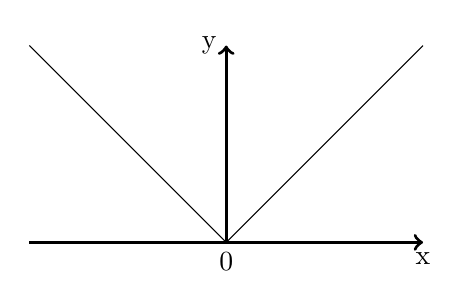
\begin{tikzpicture}[yscale=0.5, xscale=0.5]
\draw [->,very thick] (0,0) -- (0,5); \node [left] at (0,5) {y};
\draw [->,very thick] (-5,0) -- (5,0); \node [below] at (5,0) {x};

\node [below] at (0,0) {0}; 

\draw [domain=-5:5] plot (\x, {abs(\x)});

\end{tikzpicture}

Diskussion: Es gilt
$\lvert a-b \rvert =$ "`Abstand der Zahlen $a$ und $b$ auf der Zahlengeraden"'\\
\begin{tikzpicture}
\draw [->,thick] (0,0) -- (10,0);
\node [below] at (4,0) {a}; \draw [thick] (4,-0.1) -- (4,0.1);
\node [below] at (7,0) {b}; \draw [thick] (7,-0.1) -- (7,0.1);

\draw [help lines] (4,0) -- (4,1);
\draw [<->] (4,1) -- (7,1); \node [above] at (5.5,1) {$\lvert a - b \rvert$};
\draw [help lines] (7,0) -- (7,1);

\end{tikzpicture}

Speziell $\lvert a \rvert$ \dots "`Abstand von $a$ zum Ursprung $0$"'

Lösen von Ungleichungen\\
Beispiel 14 (Ungleichung von Beträgen)\\
Gesucht Lösungsmenge $L$ der reellen Zahlen, die die Ungleichung
\begin{equation}\label{Bsp14*}
\lvert x-1 \rvert < 3 + \frac{1}{2} \cdot x
\end{equation}
erfüllen.
\begin{itemize}
\item "'kritische"` Stellen: Nullstelle des Terms innerhalb der Betragszeichen, also $x=1$\\
$\curvearrowright$ Fallunterscheidung\\
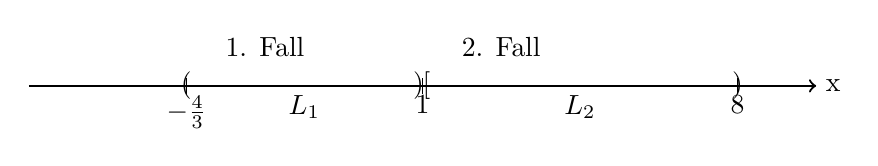
\begin{tikzpicture}
\draw [->,thick] (0,0) -- (10,0);

\node  at (3,0.5) {1. Fall};
\node  at (6,0.5) {2. Fall};
\node [below] at (5,0) {1}; \draw (5,-0.1) -- (5,0.1);
\node [right] at (10,0) {x};

\node at (2,0) {(}; \node [below] at (2,0) {$-\frac{4}{3}$}; \draw (2,-0.1) -- (2,0.1);
\node [below] at (3.5,0) {$L_1$}; \node at (4.95,0) {)};

\node at (5.05,0) {[}; \node at (9,0) {)}; \node [below] at (9,0) {8}; \draw (9,-0.1) -- (9,0.1); \node [below] at (7,0) {$L_2$};

\end{tikzpicture}\\
Dabei jeweils Beträge auflösen gemäß Definition 8


\item 1. Fall 
\begin{align*}
x<1, \quad (\ref{Bsp14*}) &\Leftrightarrow -(x-1) < 3 + \frac{1}{2} x\\
\text{d.h. } x-1<0 \quad &\Leftrightarrow -\frac{3}{2} x < 2 \quad |: (-\frac{3}{2})\\
&\Leftrightarrow \underline{\underline{x > -\frac{4}{3}}}
\end{align*}
$\curvearrowright L_1=\{x|x<1 \wedge x > -\frac{4}{3} \} = \underline{\underline{(-\frac{4}{3};1)}}$

\item 2. Fall
\begin{align*}
x \geq 1, \quad (\ref{Bsp14*}) &\Leftrightarrow (x-1) < 3 + \frac{1}{2} x\\
&\Leftrightarrow \frac{1}{2}x < 4 \quad |:\frac{1}{2}\\
&\Leftrightarrow x < 8
\end{align*}
$\curvearrowright L_2 = \{ x | x\geq 1 \wedge x < 8 \} = \underline{\underline{[1;8)}}$\\
$\curvearrowright L = L_1 \cup L_2 = \underline{\underline{(-\frac{4}{3},8)}}$
\end{itemize}

\subparagraph{Beispiel 15} (Ungleichungen mit gebrochen rationalen Termen)
\begin{equation}\label{Bsp15*}
\frac{x}{x+1} < 1 \quad |\cdot (x+1)
\end{equation}
\begin{itemize}
\item Falls $x+1 <0$ kehrt sich Ungleichungszeichen um! $\curvearrowright$ Fallunterscheidung
\item kritische Stelle(n): Nenner-Nullstellen, hier $x=-1$
\item 1. Fall: $x<-1 \quad (\ref{Bsp15*}) \Leftrightarrow x > x+1 \Leftrightarrow 0 > 1 \quad \curvearrowright$ Widerspruch\\
$x+1 < 0$\\
$\curvearrowright \underline{\underline{L_1 = \varnothing}}$

\item 2. Fall: $x > -1 \quad (\ref{Bsp15*}) \Leftrightarrow x < x+1 \Leftrightarrow 0 < 1$ (wahre Aussage)\\
$\curvearrowright L_1=\{ x | x > -1\wedge 0 < 1 \} = \underline{\underline{(-1;\infty)}}$\\
$\curvearrowright L = L_1 \cup L_2 = \underline{\underline{(-1;\infty)}}$ 
\end{itemize}

\subparagraph{Beispiel 16} (quadratische Ungleichungen)
\begin{align*}
x^2 + 3x < 10 &\Leftrightarrow (x+\frac{3}{2} )^2 - \frac{9}{4} < 10\\
&\Leftrightarrow (x + \frac{3}{2} )^2 < \frac{49}{4}\\
&\Leftrightarrow \lvert x + \frac{3}{2} \rvert < \frac{7}{2}\\
&\Leftrightarrow -\frac{7}{2} < x + \frac{3}{2} < \frac{7}{2}\\
&\Leftrightarrow \underline{\underline{-5 < x < 2}}
\end{align*}

Diskussion:
\begin{itemize}
\item In vielen Fällen ist auch ein grapischer Lösungsansatz möglich. Dabei sind geeignete Schnittpunkte (= Gleichung) exakt rechnerisch zu ermitteln, anschließend Ungleichungszeichen betrachten.
\item Im Beispiel 16: $x^2 + 3x < 10 \Leftrightarrow \underbrace{x^2 + 3x -10}_{=: f(x)} < 0$\\
Nullstellen von $f(x): x^2 + 3x -10 = 0 \curvearrowright x_1 = -5, \, x_2 = 2$\\
\begin{tikzpicture}[yscale=0.125, xscale = 0.5]
\draw [->,thick] (-6,0) -- (6,0); \node [below] at (6,0) {x};
\draw [->,thick] (0,-10) -- (0,25); \node [left] at (0,25) {y};
\draw [domain=-7:4] plot (\x, \x * \x + 3 * \x - 10);
\draw [<->, ultra thick] (-5,0) -- (2,0);
\node [below] at (-5,0) {$-5$}; \node [below] at (2,0) {$2$};
\draw (-5,-0.1) -- (-5,0.1); \draw (2,-0.1) -- (2,0.1);
\node [above] at (-1.5,0) {$L$};
\end{tikzpicture}\\
$\curvearrowright L=(-5;2)$

\end{itemize}

\subparagraph{Schranken und Grenzen}
\begin{itemize}
\item Eine Menge $M \subseteq \mathbb{R}$ heißt nach oben beschränkt, wenn es eine obere Schranke gibt, vgl. Kapitel 1.2..\\ Man kann zeigen, dass es bei dieser Ordnungsrelation $(\leq )$ auf $\mathbb{R}$ dann auch eine kleinste obere Schranke $s$ gibt.\\
(= Supremum $\sup{M}; s=\max{M} \text{ falls } s \in M)$
\item Analog: nach oben beschränkt, Infimum, Maximum
\item Falls $M$ nicht nach oben beschränkt ist, d.h. falls gilt:\\*
$\exists a \in \mathbb{R} \forall x \in M \; x \leq a \equiv \forall a \in \mathbb{R} \exists x \in M \; x > a,$ dann\\
Schreibweise $\sup{M} := \infty$
\item Analog: $\inf{M} = - \infty$
\item $M$ heißt beschränkt, falls $M$ nach oben und unten beschränkt ist.
\end{itemize}

\subparagraph{Beispiel 17} $M= \{ 1 + \frac{1}{n} | n \in \mathbb{N}^*\}$
\begin{itemize}
\item obere Schranken z.B: $3712; \pi ; 2,01$\\
kleinste obere Schranke $\sup{M}=\max{M}=2$
\item untere Schranken: z.B: $-31; 0;0,99$\\
größte untere Schranke $\inf{M}=1$\\*
$1 \notin M \curvearrowright \min{M}$ existiert nicht!
\end{itemize}

\subsubsection{Komplexe Zahlen}
Motivation: z.B. $x^2 = -1$ im Bereich der reellen Zahlen nicht lösbar $\curvearrowright$ Zahlenbereichserweiterung

\paragraph{Begriff, Rechenregeln} 
Die Menge $\mathbb{C}$ der komplexen Zahlen ist eine Obermenge der Menge der reellen Zahlen mit folgenden Eigenschaften:
\begin{enumerate}
\item $\mathbb{C}$ enthält eine Zahl $i$ mit $i^2 = -1$ (oft auch $j$ bezeichnet)
\item Jede komplexe Zahl $z$ lässt sich in der Form $z = x + i \cdot y \quad (x,y \in \mathbb{R})$ darstellen.\\
Dabei
\begin{align*}
x &= Re(z) \text{ \dots Realteil}\\
y &= Im(z) \text{ \dots Imaginärteil}
\end{align*}
\item Auf $\mathbb{C}$ werden die Operatoren $+$ (Addition) und $\cdot$ (Multiplikation) wie folgt erklärt:\\
Es seien $z_1 = x_1 + i y_1, \, z_2 = x_2 + i y_2$

Dann:\\ 
$z_1 + z_2 := x_1 + x_2 + i (y_1 + y_2)$\\*
$z_1 \cdot z_2 := x_1 \cdot x_2 - y_1 y_2 + i (x_1 y_2 + x_2 y_1)$

Die Menge $\mathbb{C}$ wird mit diesen Operationen zum Körper der komplexen Zahlen. Die arithmetischen Operationen erfolgen unter Beachtung von $i^2 = -1$ wie im Reellen.

\item Auf $\mathbb{C}$ gibt es keine natürliche Ordnungsrelation.
\end{enumerate}

Veranschaulichung: \textsc{Gauss}sche Zahlenebene\\
Zahl $z \leftrightarrow \text{ Punkt } P(x,y) \leftrightarrow \overrightarrow{OP}$ (Vector)\\
\begin{tikzpicture}
\draw [->,thick] (0,-5) -- (0,5); \node [left] at (0,5) {imaginäre Achse}; \node [left] at (0,1) {$i$}; \node [above] at (1,0) {$1$}; \node [below left] at (0,0) {$0$};
\draw [thick] (1,-0.1) -- (1,0.1);
\draw [thick] (-0.1,1) -- (0.1,1);
\draw [->,thick] (-1,0) -- (5,0); \node [below] at (6,0) {reelle Achse}; 

\draw (4,4) circle [radius=0.1]; \draw [->,very thick] (0,0) -- (4,4); \node [above] at (4,4) {$P$}; \node [right] at (4,4) {$z=x + iy$};
\node [above] at (2,2) {$\lvert z\rvert$};

\draw [->,thick] (1.5,0) arc [radius= 1.5, start angle = 0, end angle = 45]; \node [right] at (1.5,0.5) {$\varphi$};

\draw [->] (0,0) -- (4,-4);  \node [right] at (4,-4) {$\bar{z}=x - iy$}; \node [below] at (2,-2) {$\lvert z\rvert$};

\node [left] at (0,4) {$iy$}; \draw [help lines] (0,4) -- (4,4);
\node [left] at (0,-4) {$-iy$}; \draw [help lines] (0,-4) -- (4,-4);

\node [below] at (4,0) {$x$}; \draw [help lines] (4,-4) -- (4,4);

\end{tikzpicture}

\begin{itemize}
\item Betrag von $z : \: \lvert z \rvert = \sqrt{x^2 + y^2}$
\item Hauptargument von $z$: orientierter Winkel $\varphi $ von positiver x-Achse zum Strahl $\overrightarrow{OP}$ (gemessen auf kürzestem Wege!)\\
$\curvearrowright Arg \, z := \varphi (-\pi < \varphi \leq \pi )$
\item $\bar{z} = x - iy$ \dots die zu $z = x + iy$ konjugiert komplexe Zahl.
\end{itemize}

Diskussion:
\begin{enumerate}
\item Falls nicht notwendig kürzester Weg gewählt wird $\rightarrow$ Argument $arg \, z = Arg \, z + 2k\pi , \; k \in \mathbb{Z}$

z.B: $z=1-i$\\*
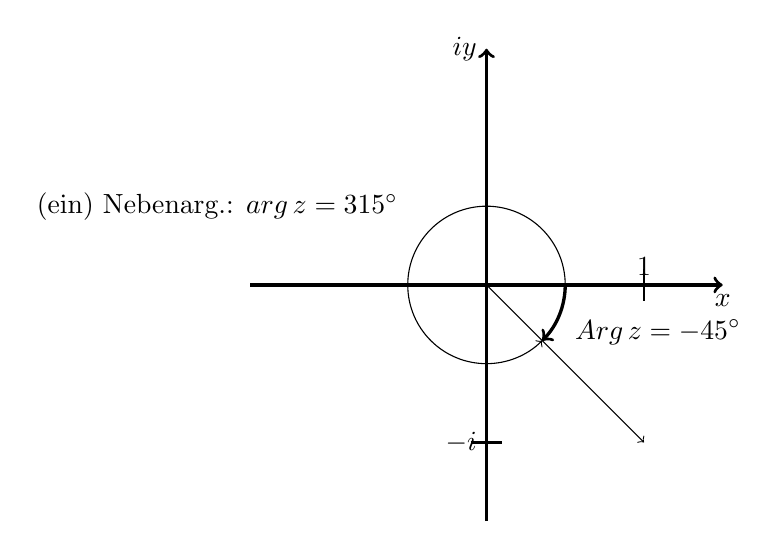
\begin{tikzpicture}[scale=2]
\draw [->,very thick] (-1.5,0) -- (1.5,0); \node [below] at (1.5,0) {$x$};
\draw [->,very thick] (0,-1.5) -- (0,1.5); \node [left] at (0,1.5) {$iy$};
\draw [thick] (1,-0.1) -- (1,0.1);
\draw [thick] (-0.1,-1) -- (0.1,-1);
\node [left] at (0,-1) {$-i$}; \node [above] at (1,0) {$1$};
\draw [->] (0,0) -- (1,-1);

\draw [->,very thick] (0.5,0) arc [radius=0.5, start angle=0, end angle= -45 ]; \node [right] at (0.5,-0.3) {$Arg \, z = -45^{\circ}$};

\draw [->] (0.5,0) arc [radius = 0.5, start angle =0, end angle =315]; \node [left] at (-0.5,0.5) {(ein) Nebenarg.: $arg \, z =315^{\circ}$};

\end{tikzpicture}

\item Berechnung von $Arg \, z (z\neq 0): \; \cos{\varphi} = \frac{x}{\lvert x \rvert} \curvearrowright$

\[ 
Arg \, z =\left\{ \begin{array}{rcl}
         \arccos(\frac{x}{\lvert z \rvert})
         & \mbox{falls}
         & y \geq 0 \\ 
         - \arccos(\frac{x}{\lvert z \rvert})  
         & \mbox{falls} 
         & y <0 \\
                \end{array}\right.
\]
\end{enumerate}

Beispiel 18: $z_1 = 3+4i, \, z_2 = -12 -5i$
\begin{enumerate}
\item Betrag u. Hauptargument
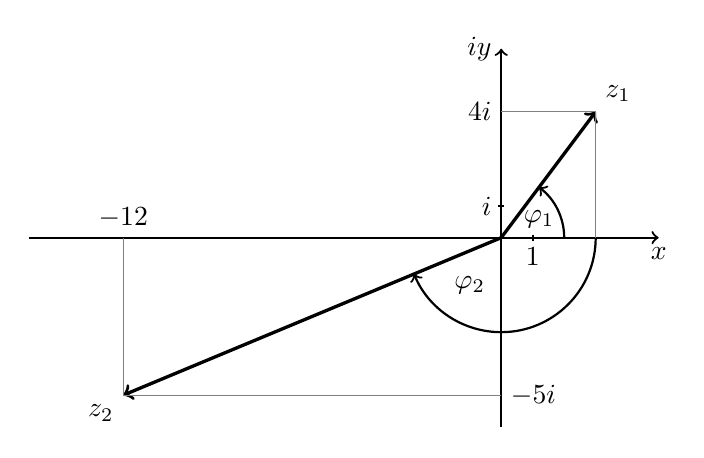
\begin{tikzpicture}[scale=0.4]
\draw [->,thick] (-15,0) -- (5,0); \node [below] at (5,0) {$x$};
\draw [->,thick] (0,-6) -- (0,6); \node [left] at (0,6) {$iy$};

\node [left] at (0,1) {$i$}; \node [below] at (1,0) {$1$};
\draw [thick] (1,-0.1) -- (1,0.1);
\draw [thick] (-0.1,1) -- (0.1,1);

\draw [->,very thick] (0,0) -- (3,4); \node [above right] at (3,4) {$z_1$}; \draw [->,thick] (2,0) arc [radius=2, start angle=0, end angle= 53.13]; \node [above] at (1.2,0) {$\varphi_1$};

\draw [->,very thick] (0,0) -- (-12,-5); \node [below left] at (-12,-5) {$z_2$}; \draw [->,thick] (3,0) arc [radius=3, start angle=0, end angle= -157.38]; \node at (-1,-1.5) {$\varphi_2$};

\draw [help lines] (3,0) -- (3,4); \draw [help lines] (0,4) -- (3,4); 
\draw [help lines] (-12,0) -- (-12,-5); \draw [help lines] (0,-5) -- (-12,-5);

\node [above] at (-12,0) {$-12$}; %\node [above] at (3,0) {$3$};
\node [left] at (0,4) {$4i$}; \node [right] at (0,-5) {$-5i$};

\end{tikzpicture}

$\lvert z_1 \rvert = \sqrt{3^2 + 4^2} = 5$\\
$\varphi_1 = Arg \, z_1 = \arccos{\frac{3}{5}} = \underbrace{53,13^\circ}_{\text{Gradmaß=DEG}}$\\
$\lvert z_2 \rvert = \sqrt{(-12)^2 + (-5)^2} = 13$\\
$\varphi_2 = Arg\, z_2 = - \arccos{\frac{-12}{13}} = -157,38^\circ$

\item Arithmetische Operationen\\
Addition: $z_1 + z_2 = -9 -i$\\
Subtraktion: $z_1 - z_2 = 15 + 9i$\\
Multiplikation: $z_1 \cdot z_2 = -36 -15i -48i -20\underbrace{i^2}_{-1} = -16 -63i$\\
Division: $\frac{z_1}{z_2} = \frac{z_1}{z_2} \cdot \frac{\bar{z_2}}{\bar{z_2}}$ (Erweiterung mit $\bar{z_2} \curvearrowright$ Nummer wird reell $z_2 \cdot \bar{z_2} = \lvert z_2 \rvert^2$)\\
also: $\frac{z_1}{z_2} = \frac{3+4i}{-12-5i} \cdot \frac{-12 +5i}{-12+5i}=-\frac{56}{169} - \frac{33}{169}i$
\end{enumerate}

\paragraph{Trigonometrische Darstellung}\textsc{Euler}sche Formel, exponentielle Darstellung\\
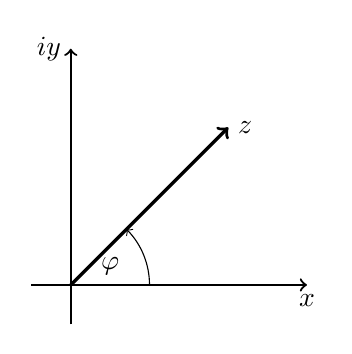
\begin{tikzpicture}
\draw [->,thick] (-0.5,0) -- (3,0); \node [below] at (3,0) {$x$};
\draw [->,thick] (0,-0.5) -- (0,3); \node [left] at (0,3) {$iy$};

\draw [->,very thick] (0,0) -- (2,2); \node [right] at (2,2){$z$};
\draw [->] (1,0) arc [radius=1, start angle=0, end angle=45]; \node [above] at (0.5,0){$\varphi$};

\end{tikzpicture} (mit $\varphi = arg\, z$ meist $\varphi = Arg\, z$)\\
$x=\lvert z\rvert \cos{\varphi}$\\*%}
$y=\lvert z \rvert \sup{\varphi}$%} Todo $z=x+iy$ (arithmetische Darstellung)

$z=\lvert z \rvert (\cos{\varphi} + i \sin{\varphi})$ (trigonometrische Darstellung.

Diskussion: $z_1 = \lvert z_1 \rvert (\cos{\varphi_1} + i \sin{\varphi_1}), z_2 = \lvert z_2 \rvert (\cos{\varphi_2} + i \in{\varphi_2})$\\*
$\curvearrowright z_1 \cdot z_2 = \lvert z_1\rvert \cdot \lvert z_2 \rvert \cdot $

Folgerung:
\begin{equation}\label{folg1}
\lvert z_1 \cdot z_2 \rvert = \lvert z_1 \rvert \cdot \lvert z_2 \rvert, \; arg(z_1 \cdot z_2 ) = arg\, z_1 + arg\, z_2
\end{equation}
\begin{equation}\label{folg2}
\lvert \frac{z_1}{z_2} \rvert = \frac{\lvert z_1\rvert}{\lvert z_2 \rvert}, \, arg(\frac{z_1}{z_2}= arg\, z_1 - arg\, z_2
\end{equation}

\subparagraph{Definition 10}
\[e^{i\varphi} := \cos{\varphi} + i \sin{\varphi}\text{ \textsc{Euler}sche Formel}\]

Diskussion:
\begin{enumerate}
\item Exponentielle Darstellung von $z$:
\[ z = \lvert z \rvert \cdot e^{i\varphi}\]
\item Wegen der Formeln (\ref{folg1}) und (\ref{folg2}) bleiben für diese Darstellung die vom Reellen hier behaupteten Potenzgesetze gültig. Insbesondere gilt die Formel von \textsc{Moivre}:
\[ z^n = (\lvert z \rvert \cdot e^{i \varphi})^n = \lvert z \rvert^n e^{in\varphi}\]
\end{enumerate}

Beispiel 19:
\begin{itemize}
\item $z_1 = \underbrace{3+4i}_{\text{arithm.}} = \underbrace{5(\cos{53,13^\circ} + i\sin{53,13^\circ})}_{\text{trigonometrisch}} = \underbrace{5 \cdot e^{i \cdot 53,13^\circ}}_{\text{exponentiell}}$\\
$z_2 = -12 -5i = 13 e^{-i \cdot 157,38^\circ}$
\item $z=-1+i$, gesucht $z^{12}$\\
$\lvert z \rvert = \sqrt{2}, \quad Arg\, z = \arccos{\frac{-1}{\sqrt{2}}} = 135^\circ = \frac{3\pi}{4} \curvearrowright z= \sqrt{2} e^{i \cdot \frac{3\pi}{4}}$\\
$\curvearrowright z^{12} = \sqrt{2}^{12} e ^{i\cdot 12 \cdot \frac{3\pi}{4}} = 2^6 e^{i \cdot 9 \pi} = 64 \cdot e^{i\pi}$\\
$\curvearrowright$ arithmetische Darstellung über die trigonometrische Darstellung\\
$z^{12} = 64 (\underbrace{\cos{\pi}}_{-1} + i \underbrace{\sin{\pi}}_{0}) = -64$
\end{itemize}
\paragraph{Spezielle Gleichungen}
\subparagraph{Quadratische Gleichung:} $z^2 + pz +q = 0 \; (p,q\in \mathbb{R}$\\*
$\Leftrightarrow (z+ \frac{p}{2})^2 = \frac{p^2}{4} - q$
\begin{enumerate}
\item 1. Fall: $\frac{p^2}{4} -q \geq 0 \curvearrowright z_{1,2} = -\frac{p}{2} \pm \sqrt{\frac{p^2}{4} -q }$
\item 2. Fall: $\frac{p^2}{4} -q < 0 \curvearrowright (z+ \frac{p}{2})^2 = \frac{p^2}{4} - q \Leftrightarrow (z +\frac{p}{2})^2 + \underbrace{q - \frac{p^2}{4}}_{=:a^2>0} = 0$\\*
$\Leftrightarrow (z+\frac{p}{2} + ia) ( z+ \frac{p}{2} -ia) = 0$
\end{enumerate}
$\curvearrowright z_{1,2} = -\frac{p}{2} \pm i \cdot \sqrt{q - \frac{p^2}{4}}$

Praktisches Vorgehen: Lösungsformel $z_{1,2} = -\frac{p}{2} \pm \sqrt{\frac{p^2}{4} -q }$ stets anwenden, im Fall 2 Formel $\sqrt{-1} = \pm i$ setzen

Beispiel 20: $x^2 + 28 +200 = 0$\\
$\curvearrowright x_{1,2} = -14 \pm \sqrt{196-200} = \underline{\underline{-14 \pm 2i}}$

\subparagraph{Kreisteilungsgleichung:} $z^n = b, \, b \in \mathbb{C},\, n\in \mathbb{N}^*$ \label{KTGL}\\*
Lösung:
\begin{itemize}
\item $b$ exponentiell darstellen $b=\lvert b \rvert e^{i\beta},\, \beta = Arg\, b$
\item \ref{KTGL} besitzt die folgenden $n$ Lösungen:\\
$z_k = \sqrt[n]{\lvert b\rvert} \cdot e^{i \frac{\beta + k \cdot 360^\circ}{n}}, \, k = 0,1,2,...,n-1$
\end{itemize}

Zum Beweis: Ansatz $z=r\cdot e^{i\varphi} \curvearrowright z^n = r^n e^{in\varphi}=\lvert b\rvert e^{i\beta}$\\
$\curvearrowright 1: r^n =\lvert b\rvert \curvearrowright r =\sqrt[n]{\lvert b \rvert}$\\*
$2: n\varphi = \beta + k \cdot 360^\circ \curvearrowright \varphi=\frac{\beta + k 360^\circ}{n}$

Beispiel 21: $z^4=-16 \quad (b=-16 \curvearrowright \lvert b \rvert b = 16, \beta = \pi = 180^\circ )$\\*
d.h. $z^4 = 16 \cdot e^{i\cdot 180^\circ}$\\
$\curvearrowright z_k= 2\cdot e^{i\frac{180^\circ + k \cdot 360^\circ}{4}}=2e^{i (45^\circ + b \cdot 90^\circ )} (k=0,1,2,3)$\\

$\begin{array}{c|c|c|c}
z_0 = 2 e^{i 45^\circ} & z_1=2e^{i 135^\circ} & z_2= 2 e^{i 225^\circ} & z_3=2 e ^{i 315^\circ}\\
=\sqrt{2} +\sqrt{2} i & =-\sqrt{2} +\sqrt{2} i&=-\sqrt{2} -\sqrt{2} i&=\sqrt{2} -\sqrt{2} i
\end{array}$

Anwendung: Faktorisierung des Polynoms $p(x) = x^4 + 16$, Nullstellen $z_0,z_1,z_2,z_3$\\*
$\curvearrowright x^4 +16 = (x-z_0)(x-z_3)(x-z_1)(x-z_2)= \underline{\underline{(x^2 - 2 \sqrt{2} x + 4) (x^2 + 2 \sqrt{2} x +4)}}$

\subparagraph{Beispiel 22}
R, C und L in Reihe (Stromkreis). $R=100\Omega C=20\mu \, F = 20\cdot 10^{-6} \frac{As}{V} \, L = 1H = 1 \frac{Vs}{A} \, \omega = 2 \pi \cdot 50 Hz$\\
Gesucht: Gesamtwiderstand $Z$.
$Z=R + R_C + R_L = R + \omega L i + \frac{1}{\omega C i} = R + i(\omega L - \frac{1}{\omega C}) = (100 + 155,04 i ) \Omega = 184,44 e^{i \cdot 57,17^\circ}$\\
Scheinwiderstand $\lvert z \rvert = 184,44 \Omega$\\
Wirkwiderstand $Re(Z) = 100 \Omega$\\
Blindwiderstand $Im(Z) = 155,04 \Omega$\\
Phasenverschiebung $Arg(Z) = 57,17^\circ$

\subsection{Reellwertige Funktionen einer reellen Veränderlichen}
\subsubsection{Elementare Funktionen (Teil 1)}
\paragraph{Polynome}
\subparagraph{Definition 1} $y=f(x)=a_nx^n + a_{n-1}x^{n-1} + \dots + a_2x^2 + a_1x + a_0$\\*
$(a_0,a_1,\dots , a_n \in \mathbb{R}, \; x \in \mathbb{R})$ heißt ganze rationale Funktion oder Polynom vom Grade $n$, falls $a_n \neq 0 $

\begin{itemize}
\item Zur Berechnung der Funktionswerte zweckmäßig: \textsc{Horner}-Schema, vgl Stellenwertsysteme
\item \textsc{Horner}-Schema liefert gleichzeitig das Ergebnis der Division durch den Linearfaktor $(x-x_0)$ vgl. Beispiel 1
\end{itemize}

Beispiel 1: $f(x) = x^5 - 2x^3 +x^2 -6, \; x_0 = 3$\\*
gesucht $f(x_0), f(x):(x-x_0)$

$\begin{array}{c|cccccc}
&1&0&-2&1&0&-6\\
x_0 = 3& & 3&9&21&66&198\\ \hline
& 1 &3&7&22&66&192=r_0 = f(3)
\end{array}$\\
$f(x):(x-3) = x^4 + 3x^3 + 7x^2 + 22x + 66 + \frac{192}{x-3}$

\subparagraph{Satz 1} Es sei $f(x)= p_n(x) = a_n x^n + \dots + a_0$ ein Polynom vom Grade $n$ (d.h. $a_n \neq 0$). Dann besitzt $f$ in $\mathbb{C}$ genau $n$ Nullstellen $x_1,\dots , x_n$ und es gilt:
\begin{equation}\label{Satz1*}
f(x)=a_n(x-x_1)\cdot (x-x_2)\dots \cdot (x-x_n) \text{ (Zerlegung in Linearfaktoren)}
\end{equation}

Diskussion: 
\begin{enumerate}
\item Falls in (\ref{Satz1*}) ein Faktor $(x-x_0)$ genau $k$-mal vorkommt $(1 \leq k \leq n)$, so heißt $x_0$ eine $k$-fache Nullstelle
\item Nicht-reelle Nullstellen sind möglich, sie treten stets paarweise ls konjugiert komplexe Zahlen auf $(x_0,\overline{x_0})$. In diesem Falle Zusammenfassung der Linearfaktoren zu einem reellen quadratischen Faktor möglich:\\*
$(x-x_0)(x-\overline{x_0} ) = x^2 - (2 Re x_0 ) \cdot x + \lvert x_0 \rvert^2$
\item Falls $a_0,a_1,\dots , a_n$ ganze Zahlen sind, so sind eventuell vorhandene ganzzahlige Nullstellen stets Teiler von $a_0$
\item Allgemeine Methoden zur Nullstellenberechnung später (Kap. 3)
\end{enumerate}

Beispiel 2: $p(x)=x^4 + x^3 - 5x^2 + x -6$, gesucht Nullstellen durch (systematisches) Probieren, vgl. Diskussion 3 $\underbrace{x_1}_{\text{Teiler von } 6: \pm 1,\pm 2,\pm 3,\pm6}=2$\\
\textsc{Horner}-Schema\\*
$\begin{array}{c|ccccc}
&1&1&-5&1&-6\\
x_1=2&&2&6&2&6\\ \hline
&1&3&1&3&0 \curvearrowright p(x)=(x-2)(x^3 + 3x^2+x+3)\curvearrowright \text{ durch Prob.: } x_2 = -3\\
x_2=-3&&-3&0&-3&\\ \hline
&1&0&1&0& \curvearrowright p(x) = (x-2)(x+3)(x^2+1) x_{3,4}=\pm i\\

\end{array}$\\
Zerlegung in Linearfaktoren: $p(x)=(x-2)(x+3)(x-i)(x+i)$

\paragraph{Gebrochenrationale Funktionen}
\subparagraph{Definition 2} $y=f(x)=\frac{p(x)}{q(x)}=\frac{a_m x^m + \dots + a_1x + a_0}{b_n x^n + \dots + b_1 x +b_0}$\\
$(a_m\neq 0 , b_n \neq 0 , \, Db(f) = \{ x \in \mathbb{R} | q(x) \neq 0\} )$ heißt gebrochenrationale Funktion.\\
$f$ heißt $\left\{ \begin{array}{rcl}
         \text{echt gebrochen}
         & \mbox{falls}
         & m < n \\ 
        \text{unecht gebrochen}
         & \mbox{falls} 
         & m \geq n \\
                \end{array}\right.$

Diskussion:
\begin{itemize}
\item Wir nehmen o.B.d.A. an, dass Zähler und Nennerpolynom keine gemeinsamen Nullstellen besitzen (ansonsten: Kürzen gemeinsamer Faktoren in Zähler u. Nummer)
\item Die Nullstellen des Nennerpolynoms heißen Polstellen der gebrochenen rationalen Funktion ($x_p$ \dots Polstellen, dann $\lim\limits_{x \rightarrow x_p} \lvert f(x) \rvert = \infty)$
\item Die Nullstellen des Zählerpolynoms sind die Nullstellen von $f(x)$
\item Verhalten von $f(x)$ bei $k$-facher Nullstelle oder Polstelle\\
Vorzeichenwechsel $\Leftrightarrow k$ ungerade
\item Polynomdivision $p(x) : q(x) = \underbrace{a(x)}_{\text{Polynom}} + \underbrace{\frac{r(x)}{q(x)}}_{\text{echt gebrochenen}}$\\*
$y=a(x)$ ist die sogenannte Asymptote.
\end{itemize}

Beispiel 3: $y=\frac{x^3+2^2}{x^2-x-2}=\frac{x^2(x+2)}{(x+1)(x-2)}=x+3 + \frac{5x +6}{x^2-x-2}$\\
$\curvearrowright$
\begin{itemize}
\item Nullstellen :$x=0 (2$-fach), $x=-2$
\item Polstellen: $x=-1, x=2$ (einfach $\rightarrow$ Vorzeichenwechsel)
\item Asymptote $y=x+3$\\*
Schnittstellen und Asymptote: $5x+6 = 0 \curvearrowright x=-1,2$
\end{itemize}
$\curvearrowright$Vereinfachte Kurvendiskussion (ohne Extremstellen, Wendestellen)
%Todo Foto 2013-12-2T16:25 ( Plot Funktionen )

\paragraph{Trigonometrische Funktionen} Übliche Definitionen der trigonometrischen Funktionen.

\subparagraph{Definition 3}
Eine Funktion $y=f(x)$ heißt periodisch, wenn es eine Zahl $p>0$ gibt mit $f(x)=f(x+p)$ (für alle $x \in Db(f)$). Die kleinste positive Zahl $p$ mit dieser Eigenschaft heißt Periode von $f$.
\subparagraph{Definition 4}
Eine Funktion $y=f(x)$ heißt
\begin{enumerate}
\item gerade, wenn $f(-x)=f(x) \quad \forall x \in Db(f)$ 
\item ungerade, wenn $f(-x)=-f(x) \quad \forall x \in Db(f)$
\end{enumerate}

Diskussion \\*
\begin{tabular}{c|c|c|c}
$y=f(x)$&$Db(f)$&Periode&Symmetrie\\ \hline
$y=\sin{x}$& $\mathbb{R}$ & $2 \pi$ & ungerade\\
$y=\cos{x}$ & $\mathbb{R}$ & $2\pi$ & gerade\\
$y=\tan{x}$ & $\mathbb{R} \backslash \{ \frac{\pi}{2} + k \pi \vert k \in \mathbb{Z} \}$ & $\pi$ & ungerade \\
$y=\cot{x}$ & $\mathbb{R} \backslash \{ k \pi \vert k \in \mathbb{Z} \}$ & $\pi$ & ungerade\\

\end{tabular}


Einige wichtige Formeln\\*
$\sin^2{x} + \cos^2{x}  = 1 \quad , \tan{x} = \frac{\sin{x}}{\cos{x}}, \cot{x}=\frac{1}{\tan{x}}$\\
$\sin{2x} = 2\sin{x}\cos{x}, \, \cos{2x} = 2 \cos^2{x}-1 = 1-2\sin^2{x}$

\paragraph{Exponentialfunktionen}
\[ y=f(x)=a^x \; (a > 0 , \, x \in \mathbb{R}\]

\begin{itemize}
\item Wichtig: Potenzgesetze, z.B. $ a^{x_1} \cdot a^{x_2} = a^{x_1 + x_2}$usw.
\item Besondere Bedeutung besitzt die Funktion $y=e^x \; (x\in \mathbb{R} )$ mit $e=\lim\limits_{n \rightarrow \infty} (1+\frac{1}{n})^n = 2,7182...$
\end{itemize}

\paragraph{Hyperbelfunktionen}
\subparagraph{Definition 5}hyperbolicus
\begin{align*}
y =& \cosh{x} :=& \frac{1}{2} (e^x + e^{-x})\; , x \in \mathbb{R}\\
y =& \sinh{x} :=& \frac{1}{2} (e^x - e^{-x})\; , x \in \mathbb{R}\\
y =& \tanh{x} :=& \frac{\sinh{x}}{\cosh{x}}\; , x \in \mathbb{R}\\
y =& \coth{x} :=& \frac{1}{\tanh{x}}\; , x \neq 0\\
\end{align*}

\subsubsection{Umkehrfunktionen}
\begin{itemize}
\item Zur Erinnerung: $y=f(x), \; x \in Db(f)$ heißt injektiv (umkehrbar eindeutig), wenn es zu jedem Bild $y \in Wb(f)$ genau ein Urbild $x \in Db(f)$ mit $ y=f(x)$ gibt, d.h.:
\[ \underbrace{y}_{\in Wb(f)} \longrightarrow \underbrace{x}_{\in Db(f)} =: f^{-1} (y)\]

Die dadurch erklärte Funktion $f^{-1} \vert Wb(f) \rightarrow Db(f)$ heißt Umkehrfunktion $f^{-1}$ ("`f oben -1 "') von $f$.\\
Es gilt: $Db(f^{-1}) = Wb(f), \; Wb(f^{-1} ) = Db(f)$
\item Bilden der Umkehrfunktion zu $y=f(x),\, x \in Db(f)$
\begin{enumerate}
\item Auflösen der Funktionsgleichung $y=f(x)$ nach $x: x=: f^{-1}(y)$ (falls dies eindeutig möglich ist, anderfalls existiert $^{-1}$ nicht!)
\item Oft erfolgt noch eine Vertauschung von $x$ und $y$\\*
$y=f^{-1}(x), \; x \in Db(f^{-1}) = Wb(f)$
\end{enumerate}
Vertauschung entspricht geometrisch einer Spiegelung an der Geraden $y=x$, vgl. Beispiel 4.
\end{itemize}

Beispiel 4: $y=f(x) = \sqrt{x} + 2, \, x \in [ 0 ; \infty)$
\begin{enumerate}
\item Auflösung nach $x: y=\sqrt{x} + 2 \Rightarrow \sqrt{x} = y-2 \Rightarrow  x= (y-2)^2 =: f^{-1}(y)$\\*
$Db(f^{-1}) = Wb(f) = [2;\infty )$
\item Vertauschung von $x$ und $y$: $y= f^{-1}(x) = (x-2)^2, Db(f^{-1})=[2;\infty)$
\end{enumerate}

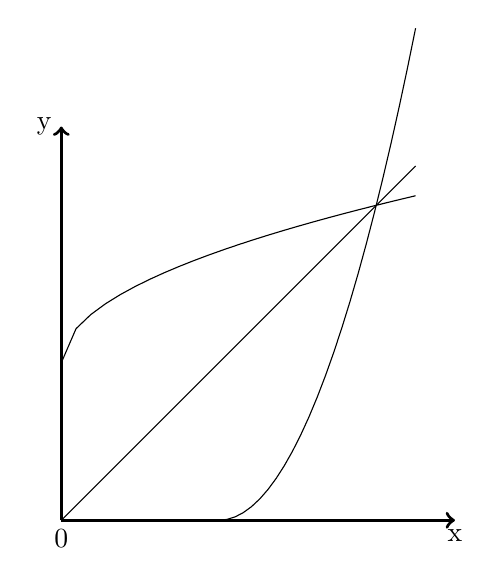
\begin{tikzpicture}[yscale=1, xscale=1]
\draw [->,very thick] (0,0) -- (0,5); \node [left] at (0,5) {y};
\draw [->,very thick] (0,0) -- (5,0); \node [below] at (5,0) {x};

\node [below] at (0,0) {0}; 

\draw [domain=0:4.5] plot (\x, {\x});
\draw [domain=0:4.5] plot (\x, {sqrt(\x) + 2});
\draw [domain=2:4.5] plot (\x, {(\x-2)*(\x-2)});
\end{tikzpicture} !$Db(f^{-1})$ ist nur $[2;\infty)$ obwohl $(x-2)^2$ für alle $x \in \mathbb{R}$ erklärt ist.

\subparagraph{Defnition 6} Die reellwertige Funktion $y=f(x)$ heißt
\begin{enumerate}
\item streng monoton wachsend, falls $x_1 < x_2 \Rightarrow f(x_1) < f(x_2)$
\item monoton wachsend (=nicht fallend), falls $x_1 < x_2 \Rightarrow f(x_1) \leq f(x_2)$
\end{enumerate}
für alle $x_1, x_2 \in Db(f)$ gilt.

Analog: streng monoton falled bzw. monoton fallend (=nicht wachsend)

\subparagraph{Satz 2} $f$ streng monoton $\Rightarrow f$ injektiv, (d.h. $f^{-1}$ existiert)

\subsubsection{Elementare Funktionen (Teil 2)}
\paragraph{Wurzel- und Logarithmusfunktionen}
\subparagraph{Definition 7}
\[ y = x^{\frac{1}{n}} = \sqrt[n]{x} \, (x\geq 0; n \in \mathbb{N}^*)\]
ist die Umkehrfunktion zu $y=x^n \, (x\geq 0, n \in \mathbb{N}^*)$\\
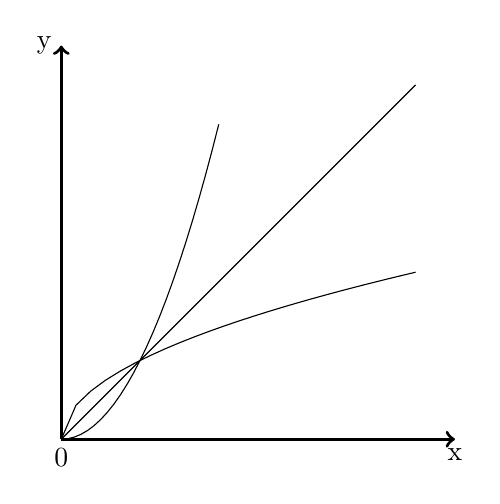
\begin{tikzpicture}[yscale=1, xscale=1]
\draw [->,very thick] (0,0) -- (0,5); \node [left] at (0,5) {y};
\draw [->,very thick] (0,0) -- (5,0); \node [below] at (5,0) {x};

\node [below] at (0,0) {0}; 

\draw [domain=0:2] plot (\x, {pow(\x,2)});
\draw [domain=0:4.5] plot (\x, {sqrt(\x)});
\draw [domain=0:4.5] plot (\x, {\x});
\end{tikzpicture}

Diskussion:
\begin{enumerate}
\item Im Bereich der reellen Zahlen ist $\sqrt[n]{x}$ nur für $x \geq 0$ erklärt, der Funktionswert selbst ist nicht negativ.
\item Lässt man in $x^{\frac{1}{n}}$ negative $x$ zu, (z.B. $ \sqrt[3]{-8} = -2$), so ergeben sich Widersprüche: $\sqrt[3]{-8}=-2 \Rightarrow -2 = (-8)^{\frac{1}{3}} = (-8)^{\frac{2}{6}}=((-8)^2)^{\frac{1}{6}} = 64^{\frac{1}{6}} = 2$\\* (die Lösungs der Gleichung $x^3 = -8$ ist natürlich $x=-2$)
\end{enumerate}

\subparagraph{Definition 8}
\[y=\log_a{x} \; (a>0, a\neq 1, x>0)\] ist die Umkehrfunktion zu $y=a^x \, (x\in \mathbb{R})$

speziell: $\lg{x}:= \log_{10}{x},\, \ln{x} := \log_e{x}$\\*
Achtung bei TR: (manchmal log=ln, auch log=lg)

Diskussion:
\begin{enumerate}
\item Log Gesetze (Basis beliebig):\\
$\log{xy} = \log{x} + \log{y}$\\
$\log{\frac{x}{y}}= \log{x} - \log{y}$\\
$\log{x^a} = a\log{x}$
\item Es gilt $a^x = e^{x \ln{a}} \; (= (\underbrace{e^{\ln{a}}}_{a})^x)$
\end{enumerate}

\paragraph{Arcusfunktionen}
Vorbetrachtung: $y=f(x) = \sin{x}$ ist nicht injektiv, also ex. keine Umkehrfunktion.\\
Aber $y=\sin{x}$ für $x\in [-2\frac{\pi}{2};\frac{\pi}{2} )$ ist injektiv, also umkehrbar.

\subparagraph{Definition 9} Umkehrfunktion der trigonometrischen Funktionen\\
\begin{tabular}{c|c|c||c}
 & Db & Wb & Umkehrfunktion von\\ \hline
$y=\arcsin{x}$ & $[-1;1]$ & $[-\frac{\pi}{2};\frac{\pi}{2}]$ & $y=\sin{x}, -\frac{\pi}{2} \leq x \leq \frac{\pi}{2}$\\ 
$y= \arccos{x}$ & $[-1;1]$ & $[0;\pi]$ & $y=\cos{x} , 0 \leq x \leq \pi$\\
$y = \arctan{x}$ & $\mathbb{R}$ & $(-\frac{\pi}{2} ; \frac{\pi}{2} )$ & $y= \tan{x}, -\frac{\pi}{2} < x < \frac{\pi}{2}$ \\
$y= \text{arccot} \,x$ & $\mathbb{R}$ & $(0;\pi)$ & $y=\cot{x}, 0<x<\pi$\\
\end{tabular}

Beispiel 5 Gesucht sind alle Lösungen der Gleichung $\tan{2x} = y$. Es sei $2x \in (-\frac{\pi}{2} + k \pi ; \frac{\pi}{2} + k\pi) \curvearrowright y=\tan{2x}=\tan{2x-k\pi} \text{ mit } 2x - k\pi \in (-\frac{\pi}{2} ; \frac{\pi}{2} )$\\
$\curvearrowright 2x - k\pi = \arctan{y} \curvearrowright \underline{\underline{ x = \frac{1}{2} (k\pi + \arctan{y}), k \in \mathbb{Z} }}$

\paragraph{Areafunktionen}
\subparagraph{Definition 10} Umkehrfunktionen der Hyperbelfunktionen\\*
\begin{tabular}{c|c|c|c}
area & Db & Wb & Umkehrfunktion von\\\hline
$y=\text{arsinh} \, x$ & $\mathbb{R}$ & $\mathbb{R}$ & $y=\text{sinh} \, x, x \in \mathbb{R}$\\
$y=\text{arcosh}\, x$ & $[1;\infty)$ & $[0;\infty)$ & $y=\text{cosh}\, x , x \geq 0$\\
$y=\text{arctanh}\, x$ & $(-1;1)$ & $\mathbb{R}$ & $y=\text{tanh}\, x , x \in \mathbb{R}$\\
$y=\text{arcoth}\, x$ & $ \mathbb{R} \backslash [-1;1]$ & $\mathbb{R} \backslash \{ 0 \} $ & $y=\text{coth}\, x, x\neq 0$\\

\end{tabular}\\
Aus der Definition 9 der Hyperbelfunktion folgt:\\*
\begin{tabular}{c|c}
$\text{arsinh}\, x = \ln{ (x + \sqrt{x^2+1})}$ & $ \text{artanh}\, x = \frac{1}{2} \ln{(\frac{1+x}{1-x} ) }$\\ \hline
$\text{arcosh}\, x = \ln{(x+\sqrt{x^2 -1})}$ & $\text{arcoth}\, x = \frac{1}{2} \ln{(\frac{x+1}{x-1})}$\\
\end{tabular}

\subsection{Lineare Algebra}
\subsubsection{Vektorräume}\label{VR}
Begriff:
\begin{enumerate}
\item \label{VR1} Gegeben seinen ein Körper $(K,+,\cdot)$, dessen Elemente Skalare heißen (meist $(\mathbb{R},+,\cdot)$ und eine \textsc{Abel}sche Gruppe $(V,\oplus)$ ($V$\dots Menge, Elemente heißen Vektoren, $\oplus$ \dots sogenannte Vektoraddition)
\item \label{VR2} Es gibt eine Abbildung $\odot$ von $K \times V \text{ in } V$, die jedem $x\in V$ und jedem $\lambda \in K$ ein Element $\lambda \odot x \in V$ zuordnet (die sogenannte Multiplikation eines Vektors mit einem Skalar) mit folgenden Eigenschaften:
\begin{itemize}
\item Distributivgesetze: $(\lambda + \mu ) \odot x = (\lambda \odot x) + (\mu \odot x)$\\
$\lambda \odot ( x \oplus y) = (\lambda \odot x ) \oplus (\lambda \oplus y)$
\item Assoziativgesetz: $(\lambda \cdot \mu) \odot x = \lambda \odot (\mu \odot x) $
\item $1\odot x = x$
\end{itemize}
\end{enumerate}
Eine Menge $V$ mit dem in (\ref{VR1}) und (\ref{VR2}) aufgeführten Operationen $\oplus$ und $\odot$ heißt Vektorraum (VR) über $K$.
Bemerkung Schreibweise meist  $\left\{ \begin{array}{rcl}
         +
         & \mbox{anstelle von}
         & \oplus \\ 
        \cdot
         & \mbox{anstelle von} 
         & \odot \\
                \end{array}\right.$

\subparagraph{Beispiel 1} Skalarbereich $K = \mathbb{R}$\\
Vektoren: Größen, die durch eine Zahlengröße (z.B. Länge) und eine Richtung charakterisiert sind (Z.B. Kräfte, Geschwindigkeiten, Translationen)

\begin{tikzpicture}
\draw [->,thick] (0,0) -- (3,3); \node [left] at (0,0) {P}; \node [above] at (1,1) {\underline{a}}; \node [right] at (3,3) {Q};

\draw [->,thick] (0,-2) -- (3,1); \node [left] at (0,-2) {R}; \node [above] at (1,-1) {\underline{a}}; \node [right] at (3,1) {S};
\end{tikzpicture} Pfeile als Repräsentation eines Vektors $\underline{a}$, Bezeichnung $\underline{a} = \overrightarrow{PQ} = \overrightarrow{RS}$ auch $\vec{a}$

Ortsvektoren: Angeheftet an einem gemeinsamen Anfangspunkt $0$ (Ursprung)

\begin{itemize}
\item Vektoraddition $\vec{a} + \vec{b}$
\item Multiplikation mit einem Skalar $\lambda \cdot \vec{a}$\\*
$\lambda > 0$ \dots gleiche Richtung\\*
$\lambda < 0$ \dots entgegengesetze Richtung\\
Länge: $\lvert \lambda \rvert \text{ -fache der Länge von }\vec{a}$
\item Subtraktion $\vec{a} - \vec{b} \;(:= \vec{a} + (-\vec{b}))$
\item Nullvektor $\vec{O}$ (Länge 0, keine Richtung)
\end{itemize}

\subparagraph{Beispiel 2} $K = \mathbb{R}, V=\{ 
\begin{pmatrix} x_1 \\ x_2 \\ \vdots \\ x_n \end{pmatrix} \vert x_1,x_2,\dots ,x_n \in \mathbb{R} \}$ (Menge der sogenannten Spaltenvektoren)
\begin{itemize}
\item Vektoraddition: $\begin{pmatrix} x_1\\ \vdots\\ x_n\end{pmatrix} + \begin{pmatrix} y_1\\ \vdots \\ y_n\end{pmatrix} := \begin{pmatrix} x_1 + y_1\\ \vdots \\ x_n + y_n\end{pmatrix}$
\item Multiplikation $\lambda \cdot \begin{pmatrix} x_1\\ \vdots\\ x_n\end{pmatrix} := \begin{pmatrix} \lambda \cdot x_1\\ \vdots\\ \lambda \cdot x_n\end{pmatrix}$
\end{itemize}

\subparagraph{Definition 1} Die Vektoren $\vec{a}_1, \dots \vec{a}_n$ heißen linear unabhängig, wenn die Gleichung \begin{equation} \label{VRDef1*} x_1 \vec{a}_1 + x_2 \vec{a}_2 + \dots + x_n \vec{a}_n = 0\end{equation}  nur die triviale Lösung $x_1=x_2=\dots = x_n=0$ besitzt.

Diskussion:
\begin{enumerate}
\item $x_1\vec{a}_1 + \dots + x_n\vec{a}_n$ heißt eine Linearkombination (LK) der Vektoren $\vec{a}_1,\dots , \vec{a}_n$
\item Falls es eine LK der Gestalt (\ref{VRDef1*} ) gibt, in der nicht alle $x_i$ gleich 0 sind, so heißen $\vec{a}_1,\dots , \vec{a}_n$ linear abhängig.\\
In diesem Falle lässt sich (wenigstens) einer der Vektoren als LK der anderen darstellen.
\end{enumerate}
\subparagraph{Definition 2} Es sei $V_1 \subseteq V$ eine nichtleere Teilmenge von $V$. Wir bezeichnen mit $L(V_1)$ die Menge aller LK von jeweils endlich vielen Vektoren aus $V_1$.\\
$L(V_1)$ heißt lineare Hülle von $V_1$

Bemerkung: $L(V_1)$ ist selbst ein VR, der von $V_1$ aufgespannte Teilraum von $V$.

\subparagraph{Definition 3}
\begin{itemize}
\item Ein VR $V$ heißt $n$-dimensional, wenn es $n$ unabhängige Vektoren $\vec{a}_1, \dots , \vec{a}_n$ gibt, die den gesamten Raum aufspannen: $V=L(\vec{a}_1, \dots ,\vec{a}_n)$
\item Die Menge der Vektoren $\vec{a}_1 , \dots ,\vec{a}_n$ nennt man in diesem Falle eine Basis von $V$.
\end{itemize}

Diskussion: In jedem VR gibt es unterschiedliche Basen, jedoch ist die Anzahl der Vektoren, die eine Basis bilden stets gleich (Dimension von VR).

\subparagraph{Satz 1} Es sei $\vec{a}_1, \dots , \vec{a}_n$ eine Basis eines VR $V$. Dann gibt es für jedes $x \in V$ eine eindeutige Darstellung der Gestalt $x=x_1\vec{a}_1 + x_2\vec{a}_2 + \dots + x_n \vec{a}_n$.

Bemerkung: Die Koeffizienten $x_1, \dots , x_n$ heißen Koordinaten von $\vec{x}$ bezüglich der Basis $\vec{a}_1, \dots , \vec{a}_n$.\\
Die Summanden $x_1 \vec{a}_1, \dots , x_n \vec{a}_n$ heißen Komponenten von $\vec{x}$ bezüglich der Basis $\vec{a}_1, \dots , \vec{a}_n$.

\subparagraph{Bespiel 3} (vlg. Beispiel 2)
Nullvektor im Raum der Spaltenvektoren: $\vec{a} = \begin{pmatrix}
0\\
0\\
\vdots\\
0
\end{pmatrix}$\\
Der Raum selbst heißt $\mathbb{R}^n$\\
Die Vektoren $\vec{e}_1 = \begin{pmatrix} 1\\0\\ \vdots \\ 0\end{pmatrix}, \vec{e}_2 = \begin{pmatrix} 0\\1\\ \vdots \\ 0\end{pmatrix}, \dots , \vec{e}_n \begin{pmatrix} 0\\0\\ \vdots \\ 1\end{pmatrix}$ des Raumes $\mathbb{R}^n$ bilden offensichtlich eine Basis von $\mathbb{R}^n$
\subparagraph{Beispiel 4} Zwei Vektoren $\vec{a}_1 \neq 0 $ und $\vec{a}_2 \neq 0$ in einer Ebene bilden genau dann eine Basis, wenn sie nicht parallel sind.

\subsubsection{Matrizen}
\subparagraph{Definition 4} Ein aus $m\cdot n $ Zahlen $a_{ij} \in \mathbb{R}$, welche in $m$ Zeilen und $n$ Spalten angeordnet sind, bestehendes Schema heißt Matrix vom Typ $(m,n)$.

$\underline{A}=
\begin{pmatrix}
a_{11} & a_{12} & \dots & a_{1n}\\
a_{21} & a_{22} & \dots & a_{2n}\\
\vdots & \vdots & \ddots & \vdots\\
a_{m1} & a_{m2} & \dots & a_{mn}\\
\end{pmatrix}
=(a_{i j}), \; \underbrace{i}_{Zeilenindex}=1,...,m \underbrace{j}_{Spaltenindex}=1,...,n$

\subparagraph{Rechenoperationen}
\subparagraph{Definition 5} $\underline{A} = (a_{ij}), \, \underline{B}=(b_{ij})$ seinen vom gleichen Typ $(m,n)$.
\begin{enumerate}
\item \label{MaRe1} $\underline{A} + \underline{B} := ( a_{ij} + b_{ij})\quad  i=1,...,m  \; j=1,...,n \text{ \dots Matr.-Addition}$
\item\label{MaRe2} $\text{Es sei } \lambda \in \mathbb{R},\, \underline{A} = (a_{ij}) \quad  i=1,...,m  \; j=1,...,n$\\*
$\lambda \cdot \underline{A} := (\lambda a_{ij}) \quad  i=1,...,m  \; j=1,...,n$
\item \label{MaRe3} $\underline{A} = (a_{ij})$ sei vom Typ $(m,n)$\\
$\underline{B} = (b_{jk})$ sei vom Typ $(n,p)$\\
$\underline{A}$ und $\underline{B}$ heißen in dieser Reihenfolge verkettet. (Spaltenzahl von $\underline{A} =$ Zeilenzahl von $\underline{B}$). Dann:\\
$\underline{A} \cdot \underline{B} = ( \sum\limits_{j=1}^n a_{ij} b_{jk} )\quad i=1,...,m \, k=1,...,p$ (Matr.-Multiplikation)\\*
Das Produkt ist also vom Typ $(m,p)$
\end{enumerate}

Diskussion: Zweckmäßig \textsc{Falk}-Schema für die Matr.-Multiplikation (vgl. Beispiel 5).

\subparagraph{Definition 6} Die aus der $(m,n)$-Matrix $\underline{A}$ durch Vertauschen von Zeilen und Spalten entstehende $(n,m)$-Matrix heißt die Transponierte von $\underline{A}$.\\*
Bezeichnung $\underline{A}^T$

Beispiel 5: $\underline{A}= \begin{pmatrix}
5&-3\\
1&4
\end{pmatrix}, \underline{B}= \begin{pmatrix}
3&6&4\\
-2&0&1
\end{pmatrix}, \underline{C} = \begin{pmatrix}
-1&5\\
0&3
\end{pmatrix}$
\begin{enumerate}
\item $\underline{A} + \underline{B}$ existiert nicht (unterschiedlicher Typ)
\item $\underline{A} + \underline{C} = \begin{pmatrix}
4&2\\
1&7 \end{pmatrix}$
\item $2 \cdot \underline{A} = \begin{pmatrix}10&-6\\ 2 & 8 \end{pmatrix}$
\item $\underline{B}^T= \begin{pmatrix}
3&-2\\
6&0\\
4&1 \end{pmatrix}$
\item $\underbrace{\underbrace{\underline{B}}_{(2,3)} \cdot \underbrace{\underline{A}}_{(2,2)}}_{3 \neq 2 \curvearrowright \text{ nicht verkettet}}$ existiert nicht
\item $\underline{A} \cdot \underline{B}$ \textsc{Falk}-Schema
%Todo 2013-12-11T11:47
\end{enumerate}

Bemerkung: Matrizen-Multiplikation ist im allgemeinen nicht kommutativ!

Diskussion (Ausgewählte Rechenregeln)
\begin{enumerate}
\item Die Menge der Matrizen vom gleichen Typ bildet mit den Operationen (\ref{MaRe1}) und (\ref{MaRe2}) aus Definition 5 einen VR (Vektorraum).
\item Falls die entsprechenden Typ-Vorraussetzungen erfüllt sind, gelten:
\begin{itemize}
\item $(\underline{A} \underline{B} ) \underline{C} = \underline{A} (\underline{B} \underline{C})$ (Assoziativgesetz)
\item $\underline{A} (\underline{B} + \underline{C}) = \underline{A} \underline{B} + \underline{A} \underline{C}$\\
$(\underline{A} + \underline{B}) \underline{C} = \underline{A} \underline{C} + \underline{B} \underline{C}$ (Distributivgesetze)
\item $(\lambda \underline{A})^T = \lambda \cdot \underline{A}^T,\, (\underline{A}^T)^T = \underline{A}$
\item $(\underline{A} + \underline{B})^T = \underline{A}^T + \underline{B}^T, \, (\underline{A} \underline{B})^T = \underline{B}^T \underline{A}^T$ 
\end{itemize}
\item Achtung: Im allg. gilt $\underline{A} \underline{B} \neq \underline{B} \underline{A}$
\item \textsc{Falk}-Schema bei fortgesetzer Multiplikation $\underline{A} \underline{B} \underline{C}$:\\
\begin{tabular}{c|c|c}
 & $\underline{B}$ & $\underline{C}$\\ \hline
$\underline{A}$ & $\underline{A} \underline{B}$ & $(\underline{A} \underline{B}) \underline{C}$
\end{tabular} oder
\begin{tabular}{c|c}
 & $\underline{C}$\\ \hline
$\underline{B}$ & $\underline{B} \underline{C}$\\ \hline
$\underline{A}$ & $\underline{A} (\underline{B} \underline{C})$
\end{tabular}
\end{enumerate}

Spezielle Matrizen:
\begin{enumerate}
\item Quadratische Matrizen: Typ $(n,n)$\\
Eine quadratische Matrix $\underline{A}$ heißt
\begin{enumerate}
\item symmetrisch, wenn $\underline{A}^T = \underline{A}$ gilt
\item obere/untere Dreiecksmatrix, wenn $a_{ij} = 0$ für $\left\{ \begin{array}{lr}
         i > j
         &   \\%Todo 2013-12-11T12:08 
         i < j
         &  \\
                \end{array}\right.$
\item Diagonalmatrix, wenn $a_{ij}=0$ für $i/neq j$
\item Einheitsmatrix $underline{E}$, wenn $a_{ij}= \left\{ \begin{array}{rcl}
         1
         & \mbox{für}
         & i = j \\ 
        0
         & \mbox{für} 
         & i \neq j \\
                \end{array}\right.$\\
(spezielle Diagonalmatrix, oft auch mit $\underline{I}$ bezeichnet)
\end{enumerate}
\item Nullmatrix $\underline{0}$ (saämtliche Elemente $=0$; nicht notwendig quadratisch)
\item Matrizen vom Typ $(n,1)$ ($n$ Zeilen, 1 Spalte) heißen (Spalten-)Vektoren\\
$\underline{a}= \begin{pmatrix} a_1\\a_2\\ \vdots \\ a_n \end{pmatrix} \in \mathbb{R}^n$, vgl. \ref{VR}\\
Es ist dann $\underline{a}^T = (a_1 | a_2 | ... | a_n)$ vom Typ $(1,n)$ (Zeilenvektor)
\end{enumerate}

Diskussion:
\begin{enumerate}
\item Die quadratischen Matrizen vom Typ $(n,n)$ bilden mit den Operationen Matr-Add. und Matr.-Multipl. einen nicht-kommutativen Ring.
\item Für quadratische Matrizen $/underline{A}$ sind Potenzen bildbar:
\[ \underline{A}^0 := \underline{E},\, \underline{A}^n = \underbrace{\underline{A} \cdot \underline{A} \cdot ... \cdot \underline{A}}_{n \text{ Faktoren}}, \; n \in \mathbb{N}^*\]
\item Falls die entsprechenden Typ-Vorraussetzungen erfüllst sind, gelten:\\
\begin{tabular}{c|c|c}
$\underline{A} \cdot \underline{E} = \underline{A}$ & $\underline{0} \cdot \underline{A} = \underline{0}$ & $\underline{A} + \underline{0} = \underline{A}$\\
$\underline{E} \cdot \underline{A} = \underline{A}$ & $ \underline{A} \cdot \underline{0} = \underline{0}$ & \\
\end{tabular}\\*
(analog 0 bzw. 1 bei reelllen Zahlen)
\item Es sei $\underline{A}$ vom Typ $(m,n),\, \underline{x} \in \mathbb{R}^n,$ d.h. vom Typ $(n,1)$\\
Dann ist $\underline{y}=\underbrace{\underline{A}}_{(m,n)}\, \underbrace{\underline{x}}_{(n,1)}$ vom Typ $(m,1)$, also $\underline{y} \in \mathbb{R}^m$\\
Durch die Zuordnung $\underline{x} \mapsto \underline{A} \, \underline{x}$ wird eine lineare Abbildung von $\mathbb{R}^n \text{ in } \mathbb{R}^m$ beschrieben. (Eine Abb. $f$ heißt linear, wenn $f(x+y) = f(x) + f(y), \, f(a\cdot x) = a \cdot f(x) \; (\forall x,y \in Db(f), \forall a \in \mathbb{R})$ gilt.)
\end{enumerate}

$\underline{y}=\underbrace{\underline{A}}_{(m,n)}\, \underbrace{\underline{x}}_{(n,1)}$ ausführlich mit \textsc{Falk}-Schema: %Todo 2013-12-11T12:33

d.h. $\begin{pmatrix}
a_{11} x_1 + \dots + a_{1n} x_n = y_1\\
\vdots \\
a_{m1} x_1 + \dots + a_{mn} x_n = y_m
\end{pmatrix} \Leftrightarrow \underline{A}\, \underline{x} = \underline{y} \implies$ Matrix-Schreibweise für ein lineares Gleichungssystem

\subsubsection{Determinanten}
\subparagraph{Definition 7} Jeder $n$-reihigen quadratischen Matrix $\underline{A}$ ist eindeutig eine Zahl $\det{\underline{A}}$, die sogenannte Determinante von $/underline{A}$, wie folgt zugeordnet:\\
$n=1 : \det(a_{11} := a_{11}$\\*
$n\geq 2: \det{ \begin{pmatrix}
a_{11} & \dots & a_{1n}\\
\vdots & \ddots & \vdots\\
a_{n1} & \dots & a_{nn} \end{pmatrix}} := a_{11} A_{11} + a_{12} A_{12} + ... + a_{1n}A_{1n}$\\
Dabei ist $A_{ij} = (-1)^{i+j} \det{\underline{U}_{ij}}$ die Adjunkte des Elements $a_{ij}$

$\underline{U}_{ij} \dots (n-1)$-reihige (Unter-)Matrix, die durch Streichen der $i$-ten Zeile und der $j$-ten Spalte von $\underline{A}$ entsteht.\\
Bezeichnung: $\det{\underline{A}} = \det{()} \underbrace{=}_{n\geq 2} \begin{vmatrix} a_{11} & \dots & a_{1n} \\ \vdots & & \vdots \\ a_{n1} & \dots & a_{nn} \\ \end{vmatrix}$

\subparagraph{Satz 2}
\begin{enumerate}
\item $\det{(\underline{A}\cdot \underline{B})} = \det{\underline{A}} \cdot \det{\underline{B}}$
\item \label{2b} $\det{(\underline{A}^T)} = \det{\underline{A}}$
\end{enumerate}
Wegen Satz 2 \ref{2b} gelten alle im folgenden für die Zeilen formulierten Eigenschaften sinngemäß auch für die Spalten.

\subparagraph{Satz 3} Eigenschaften der Determinanten
\begin{enumerate}
\item $\underline{B}$ gehe aus $\underline{A}$ durch Vertauschen zweier Zahlen hervor. Dann gilt $\det{\underline{B}} = - \det{\underline{A}}$
\item Es gilt $\det{\underline{A}} = 0$, falls zwei Zeilen elementweise proportional sind, bzw. falls alle Elemente einer Zeile gleich $0$ sind.
\item Es gilt:
$\rightarrow \begin{vmatrix}
a_{11} & \dots & a_{1n}\\
\vdots &  & \vdots\\
\lambda \cdot a_{i1} & \dots & \lambda \cdot a_{in}\\
\vdots & & \vdots\\
a_{n1} & \dots & a_{nn}\\
\end{vmatrix} =  \lambda \cdot \begin{vmatrix}
a_{11} & \dots & a_{1n}\\
\vdots & & \vdots\\
a_{i1} &\dots & a_{in}\\
\vdots & & \vdots\\
a_{n1} & \dots & a_{nn}\\
\end{vmatrix}$
\item \label{E4}Der Wert einer Determinante ändert sich nicht, wenn das $\lambda$-fache einer Zeile elementweise zu einer anderen Zeile addiert wird.
\item \label{E5} $\det{\underline{A}} = \sum\limits_{j=1}^{n} a_{ij} A_{ij}$ (Entwicklung nach $i$-ter Zeile, $i=1,...,n$)\\*
$\det{\underline{A}} = \sum\limits_{i=1}^{n} a_{ij} A_{ij}$ (Entwicklung nach $j$-ter Spalte, $j=1,...,n$)\\*
(Entwicklungssatz)
\end{enumerate}

\subparagraph{Beispiel 7} Prinzip: Nullen erzeugen mit (\ref{E4}), Entwicklungssatz  (\ref{E5}) anwenden.

\subparagraph{Anwendungen}
\begin{enumerate}
\item Vektorrechnung in $\mathbb{R}^3$, vgl. Abschnitt 1.5.5.
\item Gegebenes lineares Gleichungssystem ($n$ Gleichungen, $n$ Unbekannte)\\
Matrix-Form $\underline{A}\, \underline{x} = \underline{b}$ mit $\underline{A} = (a_{ij}), \, \underline{x} = \begin{pmatrix} x_1 \\ \vdots \\ x_n\\ \end{pmatrix}, \underline{b}= \begin{pmatrix} b_1 \\ \vdots \\ b_n\\ \end{pmatrix}$\\
$\underline{A}\, \underline{x} = \underline{b}$ besitzt genau dann eine Lösung eindeutige Lösung $\underline{x}$, wenn $\det{\underline{A}} \neq 0$.\\
In diesem Falle gilt $x_j = \frac{\det{\underline{B_j}}}{\det{\underline{A}}} \; (j=1, ... ,n)$, wobei $\underline{B}_j$ aus $\underline{A}$ hervorgeht, indem die $j$-Spalte von $\underline{A}$ durch $\underline{b}$ ersetzt wird. (\textsc{Cramer}sche Regel, theoretische Bedeutung, praktisches Vorgehen vgl. folgenden Abschnitt 1.5.4)

\end{enumerate}

\subsubsection{Lineare Gleichungssysteme, Rang einer Matrix, Inverse}
\paragraph{Das Austauschverfahren}
Gegeben: System von $m$ linearen Funktionen mit den unabhängigen Variablen $x_1,...,x_n$ und den abhängigen Variablen $y_1,...,y_m$:\\
$y_1 = a_{11} x_1 + \dots + a_{1n} x_n + a_{10}\\
\vdots\\
y_m = a_{m1} x_1 + \dots + a_{mn} x_n + a_{m0}$

\subparagraph{Beispiel 8} Betrieb, $m$ Abteilungen, $n$ Produkte $P_1,...,P_n$\\
$a_{ij}$ \dots Kosten pro Einheit von $P_j$ die in Abteilung $i$ entstehen\\
$a_{i0}$ \dots Fixkosten in Abteilung $i$\\
$x_j$ \dots produzierte Menge von $P_j$\\
$y_i$ \dots Gesamtkosten in Abteilung $i$\\

Matrix Schreibweise $\underline{y} = \underline{A} \, \underline{x} + \underline{a}$ mit $\underline{A}=(a_{ij}), \, \underline{a} = \begin{pmatrix} a_{10}\\ \vdots \\ a_{m0}\\ \end{pmatrix} \in \mathbb{R}^m$

Tabellenform: \begin{tabular}{c|cccc}
 & $x_1$ & \dots & $x_n$ & 1\\ \hline
$y_1$ & $a_{11}$ & \dots & $a_{1n}$ & $a_{10}$\\
\vdots & \vdots & & \vdots & \vdots \\
$y_m$ & $a_{m1}$ & \dots & $ a_{mn}$ & $a_{m0}$\\
\end{tabular} kurz
\begin{tabular}{c|cc}
 & $\underline{x^T}$ & 1\\ \hline
$\underline{y}$ & $\underline{A}$ & $\underline{a}$\\
\end{tabular} (T1)

Aufgaben:\begin{enumerate}
\item $\underline{x}$ vorgegeben, $\underline{y}$ ist zu berechnen (klar)
\item $\underline{y}$ vorgegeben, $\underline{x}$ ist zu berechnen (nicht immer lösbar, falls lösbar, nicht immer eindeutig lösbar)
\end{enumerate}

Lösungsprinzip: Man tausche so oft wie möglich $y_r$ gegen $x_s$ aus = Austauschschritt AS $(y_r \leftrightarrow x_s)$ Austauschverfahren

AS $y_r \leftrightarrow x_s$ bedeutet
\begin{enumerate}
\item $r$-te Zeile $y_r = \dots$ auflösen nach $x_s \curvearrowright x_s= \dots$
\item in allen anderen Zeilen $x_s$ durch die rechte Seite von $x_s \curvearrowright x_s= \dots$ ersetzen $\curvearrowright$ neue Tabelle T2
\end{enumerate}
Die Koeffizienten $a_{ij}^*$ in der neuen Tabelle, entstehen aus den alten Koeffizienten $a_{ij}$ wie folgt:

Austauschregeln\\
Abkürzungen: $p:= a_{rs}$ (Pivot)\\*
PZ \dots Pivotzeile (Zeile r)\\*
PS \dots Pivotstpalte (Spalte s)
\begin{enumerate}
\item \label{AR1} $a_{rs}^* = \frac{1}{p}$
\item \label{AR2} $a_{rj}^* = \frac{a_{rj}}{(-p)} \; (j \neq s)$\\
"`neue PZ = alte PZ / (-Pivot)"'
\item \label{AR3} $a_{is}^* = \frac{a_{is}}{p}\; (i \neq r)$ d.h.\\
"`neue PS = alte PS /Pivot"'
\item \label{AR4} $a_{ij}^* = a_{ij} + a_{is} \cdot a_{rj}^* \; (i \neq r, j \neq s)$
\end{enumerate}

Praktisches Vorgehen
\begin{enumerate}
\item Pivot kennzeichnen
\item Austauschregeln AR1 - AR4 abarbeiten.\\
Dabei für AR3 unter alter Tabelle die neue PZ als Kellerzeile schreiben.
\end{enumerate}

$\begin{pmatrix}
 & & \text{Spalte } j & \dots & \text{Spalte } s & \\
 & & \vdots & & \vdots \\
\text{Zeile } i & \dots & a_{ij} & \dots & a_{is} & \dots \\
\vdots & & \vdots & &\vdots \\
\text{Kellerzeile } K & \dots & a_{rj}^* & \dots & * & \dots \\
\end{pmatrix}$\\
$a_{ij}^* = a_{ij} + a_{is} \cdot a_{rj}^*$

\subparagraph{Varianten des Austauschverfahrens (AV)}
\begin{enumerate}
\item AVZ \dots AV mit Zeilentilgung, d.h. neue PZ in neuer Tabelle weglassen
\item AVS \dots AV mit Spaltentilgung,d.h. in neuer Tabelle neue PS weglassen\\
(nur anwendbar, wenn Variable über der wegzulassenden Spalte $=0$ ist, vgl. 1.5.4 Lineare Gleichungssysteme )
\item AVSZ \dots AVS + AVZ gleichzeitig
\end{enumerate}

\paragraph{Lineare Gleichungssysteme}
\begin{itemize}
\item Gegeben sei das lineare Gleichungssystem (in Gleichungen mit $n$ Unbekannten $x_1,...,x_n)$\\
\begin{equation} \label{GS1} \begin{array}{c} a_{11} x_1 + \dots + a_{1n} x_n = b_1\\
\vdots \\
a_{m1} x_1 + \dots + a_{mn} x_n = b_m \end{array} \end{equation}
\item Gleichungssystem (\ref{GS1}) heißt homogen, falls $b_1 = b_2 = ... = b_m = 0$, sonst inhomogen
\item Matrixform $\underline{A} \, \underline{x} = \underline{b} \Leftrightarrow \underline{A} \, \underline{x} - \underline{b} = 0$
\item Äquivalente Form: \begin{equation} \label{GS1'} \begin{array}{c} \underline{y} = \underline{A} \, \underline{x} - \underline{b} \text{ mit } \underline{y} = \begin{pmatrix} y_1 \\ \vdots \\ y_m \end{pmatrix} = \underline{0} \\ \text{Hilfsgrößen } y_1= ... = y_m = 0  \end{array} \end{equation}
\item Tabellenform:
\begin{tabular}{c|cc}
 & $\underline{x}^T$ & 1 \\ \hline
$\underline{y}$ & $\underline{A}$ & $-\underline{b}$
\end{tabular}
\item Lösungsprinzip: AVS
\begin{itemize}
\item Fall 1: Alle $y$, sind austauschbar $\Rightarrow $ (\ref{GS1}) ist lösbar, Lösung ist aus letzter Tabelle (TE) ablesbar.
\begin{tabular}{c|cc}
TE & $x_3$ & 1\\ \hline
$x_1$ & 0 & 4 \\
$x_2$ & 2 & -3 \\
\end{tabular} $x_1 = 4 \; x_2 = 2 x_3 -3 (x_3 \in \mathbb{R},$ frei wählbar)
\item Fall 2: Wenigstens ein $y_i$ ist gegen kein $x_j$ austauschbar\\
$\begin{array}{c|ccccc}
 & \text{eventuell noch nicht ausgetauschte } x_j & & & & 1\\ \hline 
\vdots \\
y_i & 0 & \dots & 0 & 0 & \alpha \\
\vdots \\
\end{array}$
$\curvearrowright y_i = \alpha $
\item Fall 2a: $\alpha = 0$ Zeile $y$, kann gestrichen werden ($0=0$)
\item Fall 2b $\alpha \neq 0 \curvearrowright$ Gleichungssystem (\ref{GS1} ) nicht lösbar (Widerspruch da $y_i = 0$ )
\end{itemize}
Diskussion: Verfahren endet also entweder im Fall 2b (unlösbar) oder in Tabelle in der kein $y_i$ mehr vorkommt (Fall 1 bzw. 2a):\\
$\begin{array}{c|ccccc} 
TE & x_{s1} & x_{s2} & \dots & x_{sq} & 1 \\ \hline
x_{r1} \\
\vdots \\
x_{rp} 
\end{array}$ (Darstellung 2)

\item $x_{r1}, ..., x_{rp}$ (ausgetausche $x_j$) \dots Basisvariable (BV)\\
$x_{s1}, ... , x_{sq}$ (nicht ausgetauschte $x_j$) \dots Nichtbasisvariable (NBV)\\
$(p + q = n )$
\item Allgemeine Lösung ergibt sich aus Endtabelle:\\
NBV frei wählbar (Parameter $\in \mathbb{R}$\\*
BV daraus berechenbar
\item Falls keine NBV vorhanden $\curvearrowright$ Lösung eindeutig
\end{itemize}
\subparagraph{Definition 8} Die Darstellung (2) heißt Basisdarstellung des lineare Gleichungssystems (\ref{GS1})

Diskussion: Aus einer Basisdarstellung (2) lassen sich weitere gewinnen durch Austausch $\underbrace{x_{ri}}_{BV} \leftrightarrow \underbrace{x_{sj}}_{NBV}$

\subparagraph{Beispiel 9}
$3 x_1 + x_2 + 2x_3 = -2$\\
$-5x_1 -3x_2 -2x_3 = -2 $ \\
$x_1 + 3x_2 -2 x_3 = 10 $\\
$\begin{array}{c|cccc}
T1 & x_1 & x_2 & x_3 & 1 \\ \hline
y_1 = 0 & 3 & 1 & 2 & 2 \\
y_2=0 & -5 & -3 & -2 & 2\\
y_3 = 0 & 1 &3 & -2 & -10 \\ \hline
K & -3 & * & -2 & -2 
\end{array}$\\
$\begin{array}{c|ccc}
T2 & x_1 & x_3 & 1\\ \hline
x_2 & -3 & -2 & -2 \\
0 & 4 & 4 & 8 \\
0 & -8 & -8 & -16 \\ \hline
K & * & -1 & -2
\end{array}$\\
$\begin{array}{c|cc}
T3 & x_3 & 1 \\ \hline
x_2 & 1 & 4 \\
x_1 & -1 & -2 \\
0 & 0 & 0 \\ \hline
\end{array}$ (Fall 2a: $0=0$ )

T3 ist Endtabelle (BV $x_1, x_2,$ NBV: $x_3$)\\
allg. Lösung: $x_2 = x_3 +4 \, x_1 = -x_3 -2 \, x_3 \in \mathbb{R}$ (frei wählbar)\\
andere Form mit Parameter $x_3 = t$: \\
$\underline{x} = \begin{pmatrix} -t -2 \\ t+4 \\ t \end{pmatrix}, t \in \mathbb{R}$

Bemerkungen:
\begin{enumerate}
\item Bei homogenen Systemen $\underline{A} \, \underline{x} = \underline{0}$ muss die 1-Spalte nicht geschrieben werden, nur "`gedacht"'
\item Die Methode AVS entspricht dem sogenannten \textsc{Gauss-Jordan}-Verfahren
\end{enumerate}

\subparagraph{Der Gausssche Algorithmus} (siehe Beispiel 10)
\begin{itemize}
\item AVSZ (Spalten und Zeilentilgung)
\item weggelassen Zeilen merken (Kellerzeilen)
\item Rückrechnung
\end{itemize}
\subparagraph{Beispiel 10}
$-x_1 + 2x_2 + 2x_3 = 4$\\
$2 x_1 + 5x_2 + 2x_3 = 4$\\
$2x_1 + x_2 -4 x_3 = -3$\\

$
\begin{array}{cc}
\begin{array}{c|cccc}
T_1 & x_1 & x_2 & x_3 & 1\\ \hline
0 & -1 & 2 & 2 & -4 \\
0 & 2 & 5 & 2 & -4\\
0 & 2 & 1 & -4 & 3 \\ \hline
x_2 & -2 & * & 4 & -3\\
\end{array}
&
\begin{array}{c|ccc}
T_2 & x_1 & x_3 & 1\\ \hline
0 & -5 & 10 & -10 \\
0 & -8 & 22 & -19\\ \hline
x_1 & * & 2 & -2\\ 
\end{array} \\
\begin{array}{c|cc}
T_3 & x_3 & 1\\ \hline
0 & 6 & -3 \\ \hline
x_3 & * & \frac{1}{2} \\ 
\end{array} & \text{\textsc{Ende AVSZ}}\\
\end{array}$\\
Rückrechnung: $T3 \curvearrowright x_3 = \frac{1}{2}$\\
$T2 \curvearrowright x_1 = 2x_3 -2 = \underline{\underline{-1}}$\\
$T1 \curvearrowright x_2 = -2x_1 + 4x_3 -3 = \underline{\underline{1}}$\\
Lösung: $\underline{\underline{\underline{x} = (-1 | 1 | \frac{1}{2} )^T}}$\\
Bemerkung: $m$ Gleichungen, $n$ Unbekannte\\
$m<n \curvearrowright$ \textsc{AVS} günstiger\\
$m \geq n \curvearrowright$ \textsc{Gauss} oder \textsc{AVS}

\paragraph{Weitere Anwendungen des AV}
\begin{enumerate}
\item Lineare Unabhängigkeit von Vektoren $\underline{a}_1, ... , \underline{a}_n \in \mathbb{R}^m$ überprüfen.\\
Ansatz: $x_1a_1 + x_2 a_2 + ... + x_n\underline{a_n} = \underline{0} \leftrightarrow \underline{A} \underline{x} = \underline{0}$ \\
mit $\underline{A} = (\underline{a}_1 | \underline{a}_2 | ... | \underline{a}_n)$\\
(homogens System, \textsc{AVS} mit Starttabelle $\begin{array}{c|c} & \underline{x}^T \\ \hline \underline{0} & \underline{A}\\ \end{array} $)
\begin{itemize}
\item Unabhängigkeit genau dann, wenn alle $x_i$ ausgetauscht werden können
\item Die zu den ausgetauschten $x_i$ (d.h. den Basisvariablen \textsc{AV}) gehörenden $\underline{a}_i$ sind unabhängig. Sie bilden eine Basis zu $L(\underline{a}_1,...,\underline{a}_n)$
\end{itemize}
\item Rang einer Matrix $\underline{A}= (a_1 | a_2 | ... | a_n) ... \text{rang}\, (\underline{A})$\\
Definition $\text{rang} \, (\underline{A}) = \dim{L (a_1, ... ,a_n)}$\\
Dimension des von den Spaltenvektoren aufgespannten Teilraumes (von $\mathbb{R}^m $)\\
Berechnung: $\text{rang}\, (\underline{A}) =$ Anzahl der ausführbaren Austauschschritte in \textsc{AVSZ} mit Starttabelle $\begin{array}{c|c} & \underline{x}^T\\ \hline \underline{y} & \underline{A} \end{array}$
\item Berechnung der Determinante einer $(n,n)$ -Matrix\\
vgl. Merkblatt LAG
\end{enumerate}

\paragraph{Die Inverse einer $(n,n)$ -Matrix}
\subparagraph{Definition 9} Es sei $\underline{A}$ vom Typ $(n,n)$. Das Gleichungssystem $\underline{y} = \underline{A}\, \underline{x}$ sei für jedes $\underline{y}$ eindeutig nach $\underline{x}$ auflösbar, d.h. $\underline{x} = \underline{B} \, \underline{y}$. Dann heißt die $(n,n)$-Matrix $\underline{B}$ Inverse zu $\underline{A}$.\\
Bezeichnung: $\underline{A}^{-1} := \underline{B}$\\
Falls $\underline{A}^{-1}$ existiert, so heißt $\underline{A}$ regulär, sonst singulär.

Bemerkungen:
\begin{enumerate}
\item $\underline{A}$ ist regulär $\leftrightarrow \det{\underline{A}} \neq 0 $
\item $\underline{A}$ regulär, dann hat $\underline{A} \, \underline{x} = \underline{b}$ die Lösung $\underline{x} = \underline{A}^{-1} \underline{b}$
\end{enumerate}

Rechenregeln: $A$ und $B$ seien regulär. Dann gelten $A A^{-1} = E,  A^{-1} A = E, (A^{-1})^{-1} = A$\\
$(AB)^{-1} = B^{-1} A^{-1}, \quad (A^T)^{-1} = (A^{-1})^T$

Bemerkung: Die Menge der regulären Matrizen vom Typ $(n,n)$ beildet mit der Operation "`Matrizen-Multiplikation"' eine (nicht \textsc{Abel}sche) Gruppe mit neutralem Element $\underline{E}$.

Verfahren zur Ermittlung der Inversen
\begin{itemize}
\item vollständiges \textsc{AV} mit Starttabelle $\begin{array}{c|c} T_1 & \underline{x}^T \\ \hline \underline{y} & \underline{A} \end{array}$\\
Fall 1: alle $x_j$ sind austauschbar $\curvearrowright \underline{A}$ regulär\footnote{nach Ordnen von Zeilen und Spalten ist $\underline{A}^{-1}$ aus TE ablesbar}
\item Probemöglichkeit $\underline{A}\, \underline{A}^{-1} = \underline{E}$
\end{itemize}

Beispiel 11:
%$\underline{A} = \begin{pmatrix} 1&2&1 \\ 1 &0 & 2\\ 1&-1&1 \end{pmatrix} \text{ ,gesucht } \underline{A}^{-1}.$\\
%$\begin{array}{ccc}
%\begin{array{c|ccc}
%T_1 &x_1 &x_2 & x_3\\ \hline
%y_1 & 1 & 2 & 1\\
%y_2 & 1 & 0 & 2\\
%y_3 & 1 & -1 & 1\\ \hline
%K & * &-2 &-1
%\end{array}
%&
%\begin{array{c|ccc}
%T_2 &y_1 &x_2 & x_3\\ \hline
%x_1 & 1 & -2 & -1\\
%y_2 & 1 & -2 & 1\\
%y_3 & 1 & -3 & 0\\ \hline
%K & -1 &2 &*
%\end{array}
%&
%\begin{array{c|ccc}
%T_3 &y_1 &x_2 & y_2\\ \hline
%x_1 & 2 & -4 & -1\\
%x_3 & -1 & 2 & 1\\
%y_3 & 1 & -3 & 0\\ \hline
%K & \frac{1}{3} &* &0
%\end{array}\\
%\begin{array{c|ccc}
%T_4 &y_1 &y_3 & y_2\\ \hline
%x_1 & \frac{2}{3} & \frac{4}{3} & -1\\
%x_3 & -\frac{1}{3} & -\frac{2}{3} & 1\\
%x_2 & \frac{1}{3} & -\frac{1}{3} & 0\\ \hline
%K & * &-2 &-1
%\end{array}
%&
%\curvearrowright \underline{A}^{-1} = \begin{pmatrix} \frac{2}{3} & -1 & \frac{4}{3} \\ \frac{1}{3} & 0 & -\frac{1}{3}\\ -\frac{1}{3} & 1 & -\frac{2}{3} \end{pmatrix} &\\
%\end{array}$

\subsubsection{Vektorrechnung im $\mathbb{R}^3$}
\paragraph{Kartesische Basis}
Einige Begriffe:
\begin{enumerate}
\item Betrag eines Vektors $\vec{a}$ : Länge des Pfeils, der $\vec{a}$ repräsentiert. Bezeichnung $\lvert \vec{a} \rvert$
\item Einheitsvektor: Vektor mit $\lvert \vec{a} \rvert = 1$
\item Zu $\vec{a} \neq \vec{0}$ gehörender Einheitsvektor $\vec{a}^0 :=  \frac{1}{\lvert \vec{a} \rvert} \cdot \vec{a}$
\item Kartesische Basis $\{\vec{i},\vec{j},\vec{k}\}$
\begin{itemize}
\item $\{\vec{i},\vec{j},\vec{k}\}$ besitzen Betrag 1
\item Sie stehen $\perp$ aufeinander
\item Sie bilden in dieser Reihenfolge ein Rechtssystem
\end{itemize}
\item Kartesisches Koordinatensystem: Fester Punkt $0$ als Urspring, kartesische Basis, damit eindeutige Zuordnung\\
$P \leftrightarrow \overrightarrow{OP} = x\vec{i} + y \vec{j} + z \vec{k} = \vec{r}$ (Ortsvektor von P)\\
Bezeichnung: $\vec{r} = x \vec{i} + y \vec{j} + z \vec{k} = \begin{pmatrix} x \\ y \\ z \end{pmatrix}$\\
bzw: $\vec{r} = \begin{pmatrix} x \\ y \\ z \end{pmatrix} = \begin{pmatrix} x_1 \\ x_2 \\ x_3 \end{pmatrix} = \vec{x}$\\
Betrag eines Vektors $\vec{a}= \begin{pmatrix} a_1 \\ a_2 \\ a_3 \end{pmatrix} \cdot \lvert \vec{a} \rvert = \sqrt{a_1^2 + a_2^2 + a_3^2}$
\end{enumerate}

\paragraph{Das Skalarprodukt}
Es sei $\varphi$ der Winkel zwischen den Vektoren $\vec{a} \text{ und } \vec{b}$\\
\subparagraph{Definition 10} Die Zahl $(\vec{a},\vec{b}) := \lvert\vec{a}\rvert \cdot \lvert \vec{b} \rvert \cdot \cos{\varphi}$ heißt Skalarprodukt der Vektoren $\vec{a}$ und $\vec{b}$.

Eigenschaften des Skalarprodukts
\begin{enumerate}
\item $(\vec{a},\vec{a}) > 0 \text{ für } \vec{a} \neq \vec{0}$
\item $(\vec{a},\vec{b}) = (\vec{b},\vec{a})$ (Symmetrie)
\item $(\lambda \vec{a} + \mu \vec{b}, \vec{c})= \lambda (\vec{a},\vec{c}) + \mu (\vec{b},\vec{c})$ (Linearität)
\end{enumerate}

\subparagraph{Satz 4} Es sei $\vec{a} = \begin{pmatrix} a_1 \\ a_2 \\ a_3 \end{pmatrix}, \vec{b} = \begin{pmatrix} b_1 \\ b_2 \\ b_3 \end{pmatrix}$.\\
Dann gilt: $(\vec{a},\vec{b}) = a_1 b_1 + a_2b_2 + a_3b_3$\\
Folgerung: $(\vec{a},\vec{b}) = \vec{a}^T \vec{b} = \vec{b}^T \vec{a}$

Anwendungen:
\begin{enumerate}
\item Projektion $\vec{a}_{\vec{b}}$ von $\vec{a}$ auf $\vec{b}: \vec{a}_{\vec{b}} = \frac{(\vec{a},\vec{b})}{\lvert \vec{b} \rvert^2} \cdot \vec{b}$\\
denn %Todo 2014-01-08T11:44
$\vec{a}_{\vec{b}} = \lvert \vec{a} \rvert \cos{\varphi} \cdot \frac{\vec{b}}{\underbrace{\lvert \vec{b} \rvert}_{\vec{b}^0}} = \frac{(\vec{a},\vec{b})}{\lvert \vec{b} \rvert^2} \cdot \vec{b}$
\item Winkel $\varphi$ zwischen 2 Vektoren: $\cos{\varphi} = \frac{(\vec{a},\vec{b})}{\lvert \vec{a} \rvert \cdot \lvert \vec{b} \rvert}$
\item Orthogonalitätskriterium
$(\vec{a},\vec{b}) = 0 \Leftrightarrow \underbrace{(\lvert \vec{a} \rvert = 0 )}_{\vec{a} = \vec{0}} \vee \underbrace{(\lvert \vec{b} \rvert = 0 )}_{\vec{b} = \vec{0}} \vee (\cos{\varphi} = 0)$\\
Vereinbarung: $\vec{0}$ orthogonal zu jedem Vektor $\curvearrowright (\vec{a},\vec{b})=0 \Leftrightarrow \vec{a} \perp \vec{b}$
\end{enumerate}

\paragraph{Das vektorielle Produkt}
\subparagraph{Definition 11} Das vektorielle Produkt (auch Kreuzprodukt) $\vec{a} \times \vec{b}$ zweier Vektoren ist ein Vektor, der eindeutig festgelegt ist durch:
\begin{enumerate}
\item $\lvert \vec{a} \times \vec{b} \rvert = \lvert \vec{a} \rvert \cdot \lvert \vec{b} \rvert \cdot \sin{\varphi}$
\item $\vec{a} \times \vec{b}$ ist senkrecht zu $\vec{a}$ und senkrecht $\vec{b}$
\item $\vec{a},\vec{b} \text{ und } \vec{a} \times \vec{b}$ bilden ein Rechtssystem
\end{enumerate}

Eigenschaften des vektoriellen Produkts: $\vec{a} \times \vec{b} = - ( \vec{b} \times \vec{a} )$\\
$\vec{a} \times (\vec{b} + \vec{c}) = \vec{a} \times \vec{b} + \vec{a} \times \vec{c}$

speziell: $\vec{a} \times \vec{a} = \vec{0}$ (stets!)\\
$\vec{i} \times \vec{j} = \vec{k},\; \vec{j} \times \vec{k} = \vec{i},\; \vec{k} \times \vec{i} = \vec{j}$\\
$\vec{j} \times \vec{i} = - \vec{k}$ usw.

\subparagraph{Satz 5} $\vec{a} \times \vec{b} = \begin{vmatrix} \vec{i} & a_1 & b_1 \\
\vec{j} & a_2 & b_2 \\
\vec{k} & a_3 & b_3 \end{vmatrix} = \begin{vmatrix} a_2 & b_2\\
a_3 & b_3 \end{vmatrix} \cdot \vec{i} - \begin{vmatrix} a_1 & b_1 \\ a_3 & b_3 \end{vmatrix} \cdot \vec{j} + \begin{vmatrix} a_1 & b_1\\ a_2 & b_2 \end{vmatrix} \cdot \vec{k}$

Anwendungen:
\begin{enumerate}
\item Flächeninhalt des von $\vec{a}$ und $\vec{b}$ aufgespannten Parallelogramms $F=\lvert \vec{a} \times \vec{b} \rvert = \lvert \vec{a} \rvert \cdot \lvert \vec{b} \rvert \cdot \sin{\varphi}$
\item Flächeninhalt eines Dreiecks $\triangle P_1 P_2 P_3$\\
$F_\triangle = \frac{1}{2} \lvert \overrightarrow{P_1P_2} \times \overrightarrow{P_1P_3}\rvert$
\item Parallelitätskriterium\\
$\vec{a} \times \vec{b} = \vec{0} \Leftrightarrow \lvert \vec{a} \times \vec{b} \rvert = 0 \Leftrightarrow ( \lvert \vec{a} \rvert = 0) \vee ( \lvert \vec{b} \rvert = 0) \vee (\sin{\varphi} = 0)$\\
Vereinbarung $\vec{0} \parallel$ zu jedem Vektor\\
$\vec{a} \times \vec{b} = \vec{0} \Leftrightarrow \vec{a} \parallel \vec{b}$
\end{enumerate}

\paragraph{Das Spatprodukt}
\subparagraph{Definition 12} Die Zahl $(\vec{a} \times \vec{b}, \vec{c})$ heißt Spatprodukt der Vektoren $\vec{a},\vec{b}$ und $\vec{c}$.\\
Eigenschaften $\vec{a} \times \vec{b}, \vec{c}) = (\vec{b} \times \vec{c}, \vec{a}) = (\vec{c} \times \vec{a}, \vec{b})$ (zyklische Vertauschung)\\
Berechnung: $(\vec{a} \times \vec{b}, \vec{c}) = \det{(\vec{a} | \vec{b} | \vec{c})} = \begin{vmatrix} a_1 & b_1 & c_1\\
a_2 & b_2 & c_2\\
a_3 & b_3 & c_3\\ \end{vmatrix}$\\
Anwendung:
\begin{enumerate}
\item Volumen des von $\vec{a}, \vec{b} \text{ und} \vec{c}$ aufgespannten Spates (Parallelotrops): $V= \lvert ( \vec{a} \times \vec{b} , \vec{c})\rvert$\\
Bemerkung: Spatprodukt $\left\{ \begin{array}{rcl}
         >0
         & \text{ Rechtssystem} \\ 
        <0
         & \text{ Linkssystem} \\
                \end{array}\right.$
\item Komplanaritätskriterium\\
$\vec{a},\vec{b} \text{ und } \vec{c}$ sind komplanar, d.h. sie liegen in $0$ angehaftet in einer Ebene, genau dann wenn: $(\vec{a} \times \vec{b},\vec{c})=0 \Leftrightarrow \vec{a},\vec{b} \text{ und } \vec{c}$ sind linear abhängig
\end{enumerate}

\paragraph{Geraden- und Ebenengleichungen}
\begin{enumerate}
\item Parameterdarstellung (P.d.) einer Geraden $g$ durch die Punkte $P_1$ und $P_2$\\
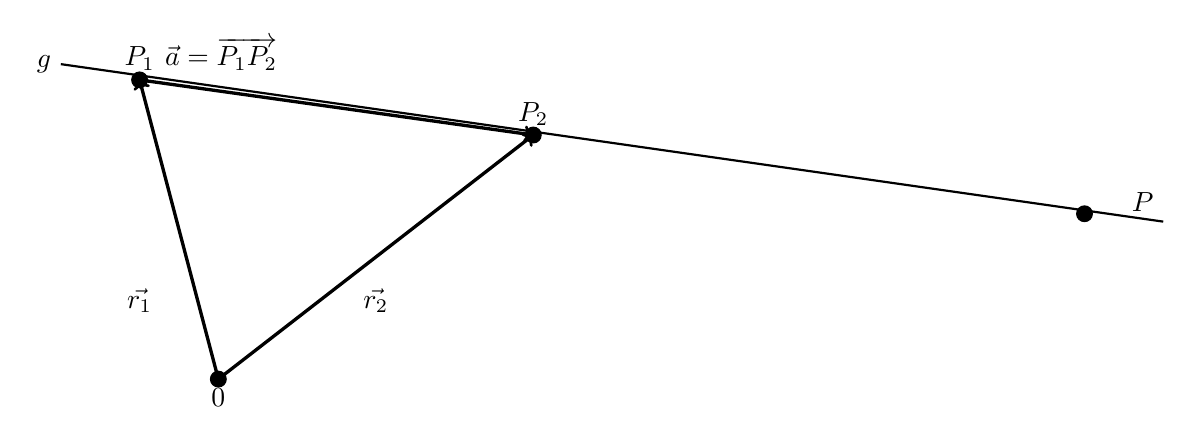
\begin{tikzpicture}[scale=2]
\node [below] at (0,0) {$0$}; \draw[fill] (0,0) circle [radius=0.05];
\draw [thick] (-1,2) -- (6,1); \node [left] at (-1,2) {$g$};

\draw[fill] (-0.5,1.9) circle [radius=0.05]; 
\node [above] at (-0.5,1.9) {$P_1$}; 
\draw [->,very thick] (0,0) -- (-0.5,1.9);
\node at (-0.5,0.5) {$\vec{r_1}$};

\draw[fill] (2,1.55) circle [radius=0.05]; 
\node [above] at (2,1.55) {$P_2$}; 
\draw [->,very thick] (0,0) -- (2,1.55);
\node at (1,0.5) {$\vec{r_2}$};

\node [above left] at (6,1) {$P$};
\draw[fill] (5.5,1.05) circle [radius=0.05]; 


\draw [->,very thick] (-0.5,1.9) -- (2,1.55); \node [above right] at (-0.4,1.9) {$\vec{a} = \overrightarrow{P_1P_2}$};
\end{tikzpicture}\\
$P \dots$ beliebiger Punkt von $g$\\
$\curvearrowright \overrightarrow{OP} = \overrightarrow{OP_1} + t \cdot \overrightarrow{P_1P_2}, t \in \mathbb{R}$\\
$\vec{r} = \vec{r_1} + t \cdot (\vec{r_2} - \vec{r_1}), t \in \mathbb{R}$\\
bzw.: $\vec{r} = \vec{r_1} = \vec{r_1} + t \cdot \vec{a}, t \in \mathbb{R}$
\item Parameterdarstellung einer Ebene $E$ durch drei Punkte $P_1, P_2, P_3$ die nicht auf einer Geraden liegen\\
$P \dots$ beliebiger Punkt von $E$.\\
$\overrightarrow{OP} = \overrightarrow{OP_1} + u \cdot \overrightarrow{P_1P_2} + v \cdot \overrightarrow{P_1P_3}, u,v \in \mathbb{R}$\\
$\vec{r} = \vec{r_1} + u \cdot (\vec{r_2} - \vec{r_1}) + v \cdot (\vec{r_3} - \vec{r_1} ) u,v \in \mathbb{R}$\\
$\vec{r} = \vec{r_1} + u \cdot \vec{a} + v \cdot \vec{b}, u,v, \in \mathbb{R}$
\item Parameterfreie Ebenengleichung\\
Normalvektor $\vec{n} (\vec{n} \neq \vec{0}, \vec{n} \perp E)$\\
$\vec{n} = \begin{pmatrix} a \\ b \\ c \end{pmatrix}, \vec{n} \perp \overrightarrow{P_0P}$\\
dabei $P(x,y,z) \dots$ beliebiger Punkt von $E$\\
$P_0 (x_0,y_0,z_0)$ fester Punkt von $E$\\
Orthogonal Kriterium $\curvearrowright (\vec{n}, \vec{r} - \vec{r_0} 0$ ausführlich:\\
$( \begin{pmatrix} a\\b\\c \end{pmatrix}, \begin{pmatrix} x-x_0\\ y - y_0 \\ z - z_0 \end{pmatrix}) = 0$ d.h. $a(x-x_0) + b\cdot (y-y_0) + c \cdot (z-z_0) = 0$\\
$\curvearrowright$ Allgemeine Form $ax+by+cz+d=0 \text{ mit } d= -ax_0 -by_0 -cz_0$
\end{enumerate}

\paragraph{Einige geometrische Grundaufgaben}
\begin{enumerate}
\item Schnitt Gerade und Ebene

Beispiel 16
\begin{equation}\label{EGG1}\text{Geg. Ebene }E: 2x -4y + z +3 = 0\end{equation}
\begin{equation}\label{EGG2}\text{Gerade } g: \begin{pmatrix}x\\y\\z\end{pmatrix} = \begin{pmatrix}3\\0\\1\end{pmatrix} + t \cdot \underbrace{\begin{pmatrix} -1 \\1 \\-2 \end{pmatrix}}_{\vec{a}}, t \in \mathbb{R} \end{equation}
Gesucht \begin{itemize}
\item Schnittpunkt $S(x_s,y_s,z_s)$
\item Schnittpunkt $\alpha$
\item $g: x=3-t y=t z=1-2t$
\end{itemize}
Einsetzen in (\ref{EGG1}) $\curvearrowright 2 \cdot (3-t) -4\cdot t + 1-2\cdot t +3 = 0$\\
$\curvearrowright -8t +10 = 0 \curvearrowright t = \frac{5}{4}$\\
Einsetzen in (\ref{EGG2}) $x=3 - \frac{5}{4} = \frac{7}{4}, y=\frac{5}{4} z= 1 - \frac{5}{2} = - \frac{3}{2}$\\
$\curvearrowright \underline{\underline{S(\frac{7}{4} | \frac{5}{4} | -\frac{3}{2} ) }}$\\
Seitenansicht\\
\begin{tikzpicture}
\node at (0,0) {E}; \draw (1,0) -- (7,0);
\node [above left]  at (3,0) {S};

\draw [->,very thick] (3,0) -- (3,4); \node [left] at (3,4) {$\vec{n}$};

\draw (1,-2) -- (6,3); \node [right] at (7,3) {g};
\node at (3.5,0.2) {$\alpha$};
\node at (3.3,0.6) {$\beta$};
\end{tikzpicture}\\
$\beta = \angle (\vec{n},\vec{a})$\\
$\alpha = \lvert 90^{\circ} - \beta \rvert$\\
\item Schnitt zweier Ebenen
\item Abstand $d(P_1,E)$ eines Punktes $P_1$ von einer Ebene $E$
\item Abstand $d(Q,g)$ eines Punktes $Q$ von einer Geraden $g$ \
$g: \vec{r} = \overrightarrow{0P_1} + t \vec{a}, t \in \mathbb{R}$\\
$L \dots $ Lotfuspunkt $ L \in g, \quad \overline{LQ} \perp g$\\
$d=$ Höhe $\overline{LQ}$ des von $\vec{a}$ und $\overrightarrow{P_1Q}$ auf gespannten Parallelogramms\\
$\curvearrowright d=d(Q,g) = \frac{\lvert \overrightarrow{P_1Q} \times \vec{a} \rvert}{\lvert \vec{a} \rvert }$ Lotfußpunkt $\overrightarrow{0L} = \overrightarrow{0P_1} + \underbrace{\overrightarrow{P_1Q}_{\vec{a}}}_{\text{Proj. von } \overrightarrow{P_1Q} \text{ auf } \vec{a}}$
\item Abstand $d(g_1,g_2)$ zweier nichtparalleler Geraden:\\
$g_1 : \vec{r} = \vec{r_1} + s \cdot \vec{a_1} (s\in \mathbb{R}$\\
$g_2 : \vec{r} = \vec{r_2} + t \cdot \vec{a_2} (t \in \mathbb{R} )$\\
$d=d(g_1,g_2) = \frac{\lvert ( \vec{r_2} - \vec{r_1} , \vec{a_1} \times \vec{a_2} ) \rvert }{\lvert \vec{a_1} \times \vec{a_2} \rvert }$
\end{enumerate}

\subsubsection{Transformationen im $\mathbb{R}^2$, homogene Koordinaten}
\begin{itemize}
\item Transformation eines Punktes $P(x,y) \mapsto P' (x',y')$ (neue Koordinaten im gleichen Koordinatensystem (= aktive Transformationen, wird im folgenden betrachtet)
\item eng verwandt: Transformation des Koordinatensystems $P(x,y)$ bleibt fest $\mapsto P'(x',y')$ neue Koordinaten in neuem Koordinatensystem (=passive Transformation)
\end{itemize}

\subparagraph{Translation} Verschiebung um den Vektor $\vec{t} = \begin{pmatrix}a \\b\end{pmatrix}$\\
\begin{equation}\label{Translation}
\begin{pmatrix} x' \\ y' \end{pmatrix} = \begin{pmatrix} x \\y \end{pmatrix} + \begin{pmatrix} a \\ b \end{pmatrix} 
\end{equation}

\subparagraph{Rotation} Zunächst Rotation um $0$, Drehwinkel $\alpha$\\
Es gilt: $x=r\cos{\varphi}, \; y=r \sin{\varphi}$\\*
($r,\varphi \dots$ Polarkoordinaten)\\
$x' = r \cos{(\varphi + \alpha)} = \underbrace{ r \cos{\varphi}}_{x} \cos{\alpha} - \underbrace{r \sin{\varphi}}_{y} \sin{\alpha}$\\
$\curvearrowright x' = x \cos{\alpha} - y \sin{\alpha}$\\*
analog $y' = x \sin{\alpha} + y \cos{\alpha}$\\
\[\begin{pmatrix} x' \\y'\end{pmatrix} = \underbrace{\begin{pmatrix} \cos{\alpha} - \sin{\alpha} \\ \sin{\alpha} \cos{\alpha} \end{pmatrix}}_{\text{Rotationsmatrix } \underline{R_{\alpha}}} \begin{pmatrix} x \\ y \end{pmatrix}\]

\subparagraph{Spiegelung} an einer Geraden $g$ durch $0$ mit dem Normaleneinheitsvektor $\vec{n} \; (\lvert \vec{n} \rvert = 1 )$\\
$\begin{pmatrix} x' \\ y' \end{pmatrix} = (\vec{E} - 2 \vec{n} \vec{n}^T ) \begin{pmatrix} x \\y \end{pmatrix}$ sogenannte \textsc{HouseHolder}-Matrix $\underline{H}$ (vgl. ÜA A6.23)

Bemerkung: Geradengleichung $ax + by + c = 0$
\[\curvearrowright \vec{n} = \frac{1}{\sqrt{a^2 + b2}} \begin{pmatrix} a \\ b \end{pmatrix}\]

\subparagraph{Skalierung (Zoom)} Koordinatenweise Streckung (oder Stauchung) von $0$ aus mit den Skalierungsfaktoren $u$ in $x$-Richtung, $v$ in $y$-Richtung
\[ \begin{pmatrix} x' \\ y' \end{pmatrix} = \underbrace{\begin{pmatrix} u & 0 \\ 0 & v \end{pmatrix}}_{\text{Skalierungsmatrix } \underline{S}_{u,v}} \begin{pmatrix} x \\ y \end{pmatrix} \]
speziell Spiegelung an x-Achse: $u=1, v=-1$\\*
speziell Spiegelung an y-Achse: $u=-1, v=1$\\

\subparagraph{Diskussion}
\begin{enumerate}
\item Drehungen um Punkte $\neq 0$ und Spiegelungen an Geraden nicht durch $0$ können durch Hintereinanderausführung einer Translation, Drehung bzw. Spiegelung und Rück-Translation realisiert.
\item Mit Ausnahme der Translation können die beschriebenen Transformationen durch Matrizen-Multiplikationen beschrieben werden (! lineare Abbildung) Zum Zwecke der Vereinheitlichung werden homogene Koordinaten eingeführt
\end{enumerate}

\subparagraph{Homogene 2D-Koordinaten} eines Punktes $P(x,y) : \begin{pmatrix} x \\ y \\1\end{pmatrix}$\\
(noch allgemeiner für $h \neq 0: \begin{pmatrix} hx\\hy\\h\end{pmatrix}$, kartesische Koordinaten ergeben sich dann durch Division durch die 3. Koordinate. Damit sind auch Zentralprojektionen beschreibar, im folgenden $h=1$)

\begin{itemize}
\item Translation in homogenen 2D-Koordinaten\\
Translationsvektor $\vec{t} = \begin{pmatrix} a \\b \end{pmatrix}$
\begin{equation}\label{HomoTrans}
\begin{pmatrix} x' \\ y' \\ 1\end{pmatrix} = \underbrace{\begin{pmatrix} 1 & 0 & a\\ 0 & 1 & b\\ 0 & 0 & 1 \end{pmatrix}}_{\text{Transformationsmatrix für homogene Koord } \underline{\tilde{T}}_{\underline{t}}} \begin{pmatrix} x \\ y \\ 1\end{pmatrix}
\end{equation}
Inverse ( $\triangleq$ Rück-Translation): $\underline{\tilde{T}}_t^{-1} = \underline{\tilde{T}}_{(-\vec{t})} = \begin{pmatrix} 1 & 0 & a\\ 0 & 1 & b\\ 0 & 0 & 1 \end{pmatrix}$
\item Rotation um $0$, Spiegelung an Geraden durch $0$, Skalierung in homogenen Koordinaten\\
Es sei $\underline{M}$ die Transformationsmatrix vom Typ $(2,2)$ für die kartesischen Koordinaten $\begin{pmatrix} x \\y \end{pmatrix}$. Dann ist die Transformationsmatrix für die homogenen Koordinaten:
\[ \underline{\tilde{M}} := \left( \begin{array}{c|c} \underline{M} & 0 \\ \hline 00 & 1\\ \end{array} \right) , \underline{\tilde{M}^{-1}} := \left( \begin{array}{c|c} \underline{M}^{-1} & 0 \\ \hline 00 & 1\end{array} \right) \]
\item Damit lässt sich die Hintereinanderausführung von beliebigen Translationen, Rotationen, Spiegelungen und Skalierungen durch Matrizenmultiplikationen darstellen (!nicht kommutativ). Die Gesamttransformation ist durch eine $(3,3)$-Matrix $\underline{\tilde{M}}$ darstellbar.
\item Mit einer weiteren Matrizenmultiplikation kann das Ergebnis der Gesamttransformation für $k$ Punkte $A(a_1,a_2),B(b_1,b_2),C(c_1,c_2), \dots $ erhalten werden:\\
$\underline{\tilde{M}} \cdot \bordermatrix{~ & A & B & C \cr
& a_1 & b_1 & c_1 & \dots \cr
&a_2 & b_2 & c_2 & \dots \cr
& 1 & 1 & 1 & \dots \cr} 
 =  \bordermatrix{~ & A' & B' & C' \cr
& a'_1 & b'_1 & c'_1 & \dots \cr
&a'_2 & b'_2 & c'_2 & \dots \cr
& 1 & 1 & 1 & \dots \cr}$ 
\end{itemize}

Beispiel 20: Das Dreieck $ABC$ mit $A(3,0), B(4,1) \text{ und } C(2,1)$ ist um seinen Eckpunkt $C$ um $60^\circ$ zu drehen (mathematisch positiv). Man gebe die Transformationsmatrix $\underline{\tilde{M}}$ für homogene 2D Koordinaten sowie das Bild an.\\
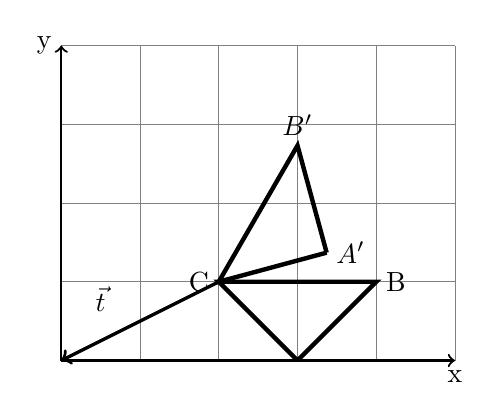
\begin{tikzpicture}
\draw[help lines] (0,0) grid (5,4); \draw [->,thick] (0,0) -- (0,4); \draw [->,thick] (0,0) -- (5,0); \node [left] at (0,4) {y}; \node [below] at (5,0) {x};

\draw [ultra thick] (3.37,1.37) -- (3,2.73) -- (2,1) -- (3.37,1.37);
\node [above] at (3,2.73) {$B'$}; \node [right] at (3.37,1.37) {$A'$};

\draw [ultra thick] (3,0) -- (2,1) -- (4,1) -- (3,0);
\node [right] at (4,1) {B}; \node [left] at (2,1) {C};

\draw [very thick, ->] (2,1) -- (0,0); \node [above] at (0.5,0.5) {$\vec{t}$};
\end{tikzpicture}
\begin{enumerate}
\item Translation um $\vec{t} = \begin{pmatrix} -2 \\-1\end{pmatrix}$\\
$\curvearrowright \underline{\tilde{T}}_{\vec{t}} = \begin{pmatrix}
1 & 0 & -2 \\
0 & 1 & -1 \\
0 & 0 & 1
\end{pmatrix}$
\item Rotation um $\alpha = 60^\circ$ um $0$\\
$\underline{R}_\alpha =  \begin{pmatrix} \cos{\alpha} & -\sin{\alpha}\\
\sin{\alpha} & \cos{\alpha} \end{pmatrix} = \begin{pmatrix}
\frac{1}{2} & -\frac{1}{2} \sqrt{3} \\
\frac{1}{2} \sqrt{3} & \frac{1}{2} \end{pmatrix}$\\
$\curvearrowright \underline{\tilde{R}}_\alpha = \begin{pmatrix}
\frac{1}{2} & -\frac{1}{2} \sqrt{3} & 0 \\
\frac{1}{2} \sqrt{3} & \frac{1}{2} & 0 \\
0 & 0 & 1 \end{pmatrix}$
\item Rücktranslation $\underline{\tilde{T}}_{\vec{-t}} = \begin{pmatrix}
1 & 0 & 2 \\
0 & 1 & 1 \\
0 & 0 & 1
\end{pmatrix}$
\end{enumerate}
$\curvearrowright \underline{\tilde{M}} = \underline{\tilde{T}}_{(-\vec{t})} \underline{R}_{\alpha} \underline{\tilde{T}}_{\vec{t}} $\\
$\curvearrowright A'(3,37;1,37), B'(3;2,73), C'(2;1)$

Bemerkung: Analoges Vorgehen im $\mathbb{R}^3$, homogene Koordinaten $x,y,z,1.$ Spiegelung an einer Ebene mit Normalen-Einheitsvektor $\vec{n}$ mit $(3,3)$- \textsc{HouseHolder}-Matrix.

Rotation um eine beliebige Achse (durch $0$) durch $3$ Drehungen um die Koordinatenachsen ersetzbar, \dots .\\
Anschließend erfolgt Projektion in $\mathbb{R}^2$

\subsubsection{Eigenwerte und Eigenvektoren}
Es sei $\underline{A}$ eine $(n,n)$-Matrix.

\subparagraph{Definition 13} Die Zahl $\lambda \in \mathbb{C}$ heißt Eigenwert (EW) der quadratischen Matrix $\underline{A}$, falls die Gleichung $\underline{A} \, \underline{x} = \lambda \underline{x}$ nicht triviale Lösungen $\underline{x} \quad (x \neq 0 )$ besitzt. Diese heißen dann Eigenvektoren (EV) von $\underline{A}$ zum EW $\lambda$.

Diskussion:
\begin{enumerate}
\item $\underline{A} \, \underline{x} = \lambda \underline{x} \Leftrightarrow (\underline{A} - \lambda \underline{E} ) \underline{x} = \underline{0}$ (homogenes System), d.h. nicht triviale Lösungen existieren genau dann, wenn $\det{(\underline{A} - \lambda \underline{E} )} = 0$ (charakteristische Gleichung) gilt.\\
\item $\curvearrowright$ Vorgehensweise zur Ermittlung von EW zu EV von $\underline{A}$
\begin{itemize}
\item charakteristische Gleichung lösen ($n \text{ im allg. komplexe Lösungen } \lambda_1 , \dots , \lambda_n ) \curvearrowright \text{ EW}$
\item Gleichungssysteme $\underline{A} - \lambda_i \underline{E} ) \underline{x} = \underline{0}$ lösen $\curvearrowright$ EV
\end{itemize}
\end{enumerate}

Im folgenden werden nur symmetrische $(n,n)$-Matrizen $\underline{S}$ betrachtet, d.h. $\underline{S}^T = \underline{S}$

\subparagraph{Satz 6} Es sei $\underline{S}$ symmetrische $(n,n)$-Matrix. Dann gilt:
\begin{enumerate}
\item Alle EW von $\underline{S}$ sind reell.
\item Zu verschiedenen EW $\lambda_1 \text{ bzw. } \lambda_2 (\lambda_1 \neq \lambda_2 )$ gehörende EV $\vec{v}_1 \text{ bzw. } \vec{v}_2$ sind orthogonal (vgl. Diskussion)
\item Es gibt eine Basis des Raumes $\mathbb{R}^n$, die aus $n$ paarweise orthonormierten EV $\vec{v}_1, \dots , \vec{v}_n$ von $\underline{S}$ besteht (vgl. Diskussion)
\item Es sei $\underline{V} = (\vec{v}_1; \vec{v}_2; \dots ; \vec{v}_n ) $ eine Matrix, die aus $n$ paarweise orthonormierten EV von $\underline{S}$ zusammengesetzt ist. Dann gilt:
\begin{itemize}
\item $\underline{V} \, \underline{V}^T = \underline{V}^T \underline{V} = \underline{E}$ (d.h. $\underline{V}^{-1} = \underline{V}^T$, $\underline{V}$ nennt sich auch orthogonale Matrix.
\item $\underline{V}^T \underline{S} \, \underline{V} = \begin{pmatrix}
\lambda_1 & 0 & \dots & 0\\
0 & \lambda_2 & \dots & 0\\
\vdots & \vdots & \ddots & \vdots \\
0 & 0 & \dots & \lambda_n \\
\end{pmatrix} = \Lambda$ (Diagonalmatrix)\\
$\curvearrowright \underline{S} = \underline{V} \, \underline{\Lambda} \underline{V}^T$
\item Es gilt $\underline{S}^{-1} = \underline{V} \, \underline{\Lambda}^{-1} \underline{V}^T$ (dabei $\underline{\Lambda}^{-1} = \begin{pmatrix}
\frac{1}{\lambda_1} & 0 & \dots & 0\\
0 & \frac{1}{\lambda_2} & \dots & 0\\
\vdots & \vdots & \ddots & \vdots \\
0 & 0 & \dots & \frac{1}{\lambda_n} \\
\end{pmatrix} \text{ und } \underline{S}^m = \underline{V} \underline{\Lambda}^m \underline{V}^T$
\end{itemize}

\end{enumerate}

Diskussion
\begin{enumerate}
\item Übertragung der Begriffe orthogonal, Länge eines Vektors aus $\mathbb{R}^3 \text{ bzw. } \mathbb{R}^2 \text{ in } \mathbb{R}^n$
\item $\vec{a}, \vec{b} \in \mathbb{R}^n$ heißen orthogonal, wenn $\vec{a}^T \vec{b} = \sum\limits_{i=1}^n a_i b_i = 0$ gilt, Skalarprodukt
\[ (\vec{a},\vec{b}) = \sum\limits_{i=1}^n a_i b_i\]
\item Betrag (Norm) eines Vektors $\lvert \vec{a} \rvert = \sqrt{\sum\limits_{i=1}^n a_i^2}$
\item paarweise orhtonomiert bedeutet 
\[ (\vec{v}_i,\vec{v}_j) = \left\{ \begin{array}{rcl}
         1
         & \mbox{falls}
         & i=j  \text{ d.h. } \lvert v_i \rvert = 1 (\forall i)\\ 
        0
         & \mbox{falls} 
         & i \neq j \\
                \end{array}\right.\]
\end{enumerate}

\subparagraph{Definition 13} \begin{enumerate}
\item $\underline{A} \, \vec{x} = \lambda \vec{x}, \, \vec{x} \neq \vec{0},\, \lambda \text{ EW }, \vec{x} \text{ EV}$
\item Veranschaulichung im Fall $n=2$:\\
Die symmetrische Matrix $\underline{A}$ habe die EW $\lambda_1$ und $\lambda_2$ und orthonormierte EV $\vec{v}_1$ und $\vec{v}_2, \underline{V} = (\vec{v}_1|\vec{v}_2)$\\
Es gilt: \\
$\underline{A} \vec{v}_1 = \lambda_1 \vec{v}_1$\\*
$\underline{A} \vec{v}_2 = \lambda_2 \underline{v}_2$\\
D.h. $\underline{A}$ bewirkt eine Skalierung mit den Faktoren $\lambda_1$ und $\lambda_2$ in Richtung $\vec{v}_1$ bzw. $\vec{v}_2$.

\end{enumerate}

\subparagraph{Definition 14} Es sei $\underline{S}$ eine reelle symmetrische Matrix vom Typ $(n,n)$. Die Funktion
\[ y= Q(\vec{x}) := \underbrace{\vec{x}^T}_{(1,n)} \underbrace{\underline{S}}_{(n,n)} \underbrace{\vec{x}}_{(n,1)} \quad (\vec{x} \in \mathbb{R}^n, y \in \mathbb{R})\]
heißt quadratische Form.

Diskussion:
\begin{enumerate}
\item Im Falle $n=2$ stellt $Q(\vec{x} ) = \text{ const. }$ (bzw. $ Q(\vec{x}) + \vec{a}^T \vec{x} = \text{ const. } )$ eine Kurve 2. Ordnung dar. Deren Gestalt kann durch die sogenannte Hauptachsentransformation ermittelt werden (vgl. Diskussion 3)
\item Ausführliche Schreibweise $\vec{x} = \begin{pmatrix} x \\y \end{pmatrix}, \underline{S} = \begin{pmatrix} s_{11} & s_{12}\\ s_{21} & s_{22} \end{pmatrix} \text{ mit } s_{12} = s_{21}$
\begin{equation}\label{Def14D2}
Q(x,y) = (x|y) \begin{pmatrix} s_{11} & s_{12} \\ s_{12} & s_{22} \end{pmatrix} \begin{pmatrix} x \\ y \end{pmatrix} = s_{11}x^2 + 2 s_{12} xy + s_{22} y^2
\end{equation}
\item Es seien $\lambda_1$ und $\lambda_2$ die EW von $\underline{S}$ und $\vec{v}_1$ bzw. $\vec{v}_2$ orthonomierte EV. Für einen beliebigen Vektor $\vec{x} = \begin{pmatrix} x \\y \end{pmatrix} \in \mathbb{R}^2$ seien $x^*,y^*$ die Koordinaten bzgl. der Basis 
\begin{equation} \label{Def14D31} \vec{v}_1,\vec{v}_2 : \vec{x} = x^* \cdot \vec{v}_1 + y^* \cdot \vec{v}_2 = (\vec{v}_1|\vec{v}_2 ) \begin{pmatrix} x^* \\ y^* \end{pmatrix} = \underline{V} \vec{x}^*
\end{equation} mit $\vec{x}^* = \begin{pmatrix} x* \\ y* \end{pmatrix}$. Dann gilt
\begin{equation}\label{Def14D32}
Q(x,y) = \lambda_1 x^{*2} + \lambda_2 y^{*2}
\end{equation} (Darstellung bzgl. der sog. Hauptachsen)

Denn: $Q(x,y) = \vec{x}^T \underline{S} \underline{x} = (\underline{V} \underline{x}^*)^T \underline{S} \underline{V} \vec{x}^* = \vec{x}^{*T} \underbrace{\underline{V}^T  \underline{S} \underline{V} \vec{x}^*}_{\Lambda \text{ vgl. Satz 6}} = (\vec{x}^* | \vec{y}^* ) \begin{pmatrix} \lambda_1 & 0 \\ 0 & \lambda_2 \end{pmatrix} \begin{pmatrix} x^* \\ y^* \end{pmatrix} = \lambda_1 x^{*2} + \lambda_2 y^{*2}$
\end{enumerate}

Beispiel 21: $Q(x,y) = 13x^2 - 32xy + 37y^2 = 45$\\
Welche Kurve?
\begin{itemize}
\item Matrix $\underline{S}$ (vgl. (\ref{Def14D2}), $\underline{S}= \begin{pmatrix} 13 & -16 \\ -16 & 37 \end{pmatrix} \quad ( s_{12} = -16 )$
\item charakteristische Gleichung: $\det{(\underline{S} - \lambda \underline{E})} \begin{vmatrix} 13-\lambda & -16 \\ -16 & 37 - \lambda \end{vmatrix} = 0 \Leftrightarrow \lambda^2 - 50 \lambda + 225 = 0 \curvearrowright \underline{\underline{\lambda_1 = 5, \lambda_2 = 45}} (\text{EW})$
\item EV zu $\lambda_1=5: 8x - 16y = 0 \curvearrowright x = 2y, y=t, x=2t (-16x + 32y = 0) \curvearrowright \underline{\underline{\begin{pmatrix} x \\y \end{pmatrix} = \begin{pmatrix} 2t \\ t \end{pmatrix} = t \cdot \begin{pmatrix} 2 \\ 1 \end{pmatrix}, t \neq 0 }}$
\item EV zu $\lambda_2 = 45: (-32x -16y = 0 ), -16x -8y = 0 \curvearrowright y=-2x, x=u, y= -2u \curvearrowright \underline{\underline{ \begin{pmatrix} x \\y \end{pmatrix} = \begin{pmatrix} u \\ -2u \end{pmatrix} = u \cdot \begin{pmatrix} 1 \\ -2 \end{pmatrix}, u \neq 0}}$
\item orthonormierte EV z.B: $\vec{v}_1 = \frac{1}{\sqrt{5}} \begin{pmatrix} 2 \\ 1 \end{pmatrix}, \vec{v}_2 = \frac{1}{\sqrt{5}} \begin{pmatrix}-1\\2\end{pmatrix}$ (Rechtssystem)
\end{itemize}
(\ref{Def14D32}) $\curvearrowright Q(x,y)= \lambda_1 x^{*2} + \lambda_2^{*2} = 5 x^{*2} + 45 y^{*2} = 45 \Leftrightarrow \frac{x^{*2}}{3^2} + \frac{y^{*2}}{1^2} =1$ Ellipse mit Halbachsen $a=3,b=1$

\section{Folgen, Reihen, Grenzwerte}
\subsection{Zahlenfolge}
\subsubsection{Grenzwerte von Zahlenfolgen}
\subparagraph{Definition 1}: Es sei $n_0 \in \mathbb{N}$. Eine Funktion $f$ mit $Db(f) = \{ n \in \mathbb{N} | n \geq n_0 \} \text{ und } Wb(f) \subseteq \mathbb{R}$ heißt reelle Zahlenfolge.\\
Schreibweisen: \[a_n := f(n)\]
$(a_n)_{n\geq n_0} = (a_{n_0}, a_{n_0 +1 }, a_{n_0 +2 },\dots)$\\
Oft ist $n_0 = 0$ oder $ n_0=1$.

\subparagraph{Beispiel 1}
\begin{enumerate}
\item $a_n = (-1)^n \cdot n (n \in \mathbb{N}), (a_n) = (0,-1,2,-3,4,-5,\dots)$
\item $a_0 = -1, a_n = n \cdot a_{n-1} ( n \in \mathbb{N}^*)$ (rekursive Definition)\\
$(a_n)= (-1,-1,-2,-6,-24,-120,\dots), a_n= -n!$
\item $a_n= \sum\limits_n \frac{3}{10^n} (n\in\mathbb{N}^*), (a_n) = (0,3;0,33;0,333;\dots)$
\item $a_n = a + (-1)^n \cdot \frac{1}{n^2} (n \in \mathbb{N}^*), (a_n) = (0,\frac{5}{4},\frac{8}{9},\frac{17}{16},\frac{24}{25},\dots)$
\end{enumerate}

\subparagraph{Definition 2}
\begin{itemize}
\item $(a_n)$ heißt konvergent, wenn es eine Zahl $a \in \mathbb{R}$ gibt mit:
\[\forall \epsilon >0 \; \exists n_0(\epsilon)\; (n_0 \in \mathbb{N}), \forall n \in \mathbb{N}_{\geq n_0(\epsilon)}: \lvert a_n - a \rvert < \epsilon\]
\item Die Zahl $a$ heißt Grenzwert von $(a_n)$.\\
Schreibweise $a= \lim\limits_{n \to \infty} a_n$
\item $(a_n)$ heißt divergent, wenn $(a_n)$ nicht konvergent ist.

Diskussion 
\item Folgen aus Beispiel 1\\
$\begin{array}{l|c|r}
\text{Folge} & \text{Monotonie} & \text{Beschränktheit}\\ \hline
a) \; a_n = (-1)^n n & - & - \\
b) \; a_n = -n! & \text{streng monoton fallend (ab } n=1) & -\\
c)\; a_n = \frac{3}{10} + \dots + \frac{3}{10^n} & \text{streng monoton wachsend} & 0,3 \leq a_n < \frac{1}{3} \\
d)\; a_n = 1 + (-1)^n \cdot \frac{1}{n^2} & - & 0 \leq a_n \leq \frac{5}{4}\\

\end{array}$
\end{itemize}

\subparagraph{Satz 1} Jede konvergente Folge ist beschränkt.
\subparagraph{Satz 2} Jede monotone und beschränkte Folge ist konvergent.

\subparagraph{Definition 5} $(a_n)$ heißt bestimmt divergent gegen $\left\{ \begin{array}{rc}
         +
         & \infty \\ 
        -
         & \infty\\
                \end{array}\right.$
falls gilt: $\forall C \in \mathbb{R} \exists n_0 (C) \forall n \geq n_0 (C) \left\{ \begin{array}{lc} a_n & > C \\ a_n & <C\\ \end{array} \right. $
\subparagraph{Satz 3} Jede unbeschränkte, monoton $\left\{ \begin{array}{l} \mbox{wachsende} \\ \mbox{fallende} \end{array} \right.$ Folge ist bestimmt divergent gegen $\left\{ \begin{array}{rc}
         + & \infty \\ 
        - & \infty\\
\end{array}\right.$\\
Schreibweise $\lim\limits_{n \to \infty} a_n = \left\{ \begin{array}{rc}
         + & \infty \\ 
        - & \infty\\
\end{array}\right.$

\subparagraph{Beispiel 2} \begin{enumerate}
\item Bsp 1 c) $a_n = \frac{3}{10} + \dots + \frac{3}{10^n}, (a_n)$ ist monoton wachsend und beschränkt $\underbrace{\Rightarrow}_{\text{Satz 2}} (a_n)$ ist konvergent, $\lim\limits_{n \to \infty} a_n = \frac{1}{3}$
\item Bsp 1 b) $a_n = -n!, (a_n)$ ist monoton fallend und unbeschränkt $\underbrace{\Rightarrow}_{\text{Satz 3}} (a_n)$ ist bestimmt divergent, $\lim\limits_{n \to \infty} a_n = - \infty$
\end{enumerate}

\subparagraph{Diskussion} Eine divergente Folge, die nicht bestimmt divergent ist, heißt unbestimmt divergent, z.B. Folge aus Beispiel 1a) $a_n = (-1)^n \cdot n$

\subparagraph{Einige wichtige Grenzwerte}
\begin{enumerate}
\item $\lim\limits_{n \to \infty} ( 1 + \frac{1}{n})^n = e$
\item $\lim\limits_{n \to \infty} \sqrt[n]{n} = 1$
\item $\lim\limits_{n \to \infty} \frac{\ln{n}}{n} = 0$
\item $\lim\limits_{n \to \infty} \sqrt[n]{a} = 1 \; (a > 0)$
\end{enumerate}

\subparagraph{Rechenregeln}(Grenzwertsätze)

\subparagraph{Satz4} $(a_n) \text{ und } (b_n)$ seien konvergente Folgen mit
$\lim\limits_{n \to \infty} a_n = a \text{ und } \lim\limits_{n \to \infty} b_n = b$.\\
Dann gilt
\begin{itemize}
\item $\lim\limits_{n \to \infty} ( a_n + b_n) = a+b,\quad \lim\limits_{n \to \infty} ( c \cdot a_n) = c \cdot a$
\item $\lim\limits_{n \to \infty} (a_n \cdot b_n) = a \cdot b, \quad \lim\limits_{n \to \infty} \frac{a_n}{b_n} = \frac{a}{b} \; (b \neq 0 )$
\end{itemize}

\subparagraph{Beispiel 3}
\begin{enumerate}
\item $a_n = \frac{2n^2 -1}{3n^2+n} ( n= 1,2,3,...)$\\
$a_n = \frac{n^2(2-\frac{1}{n^2})}{n^2 (3 + \frac{1}{n})} = \frac{2- \frac{1}{n^2}}{3+ \frac{1}{n}} \curvearrowright \lim\limits_{n\to \infty} a_n = \frac{2}{3}$\\
Ausklammern der jeweils höchsten Potenzen in Zähler und Nenner.
\item $a_n = n \cdot ( \sqrt{n^2 +1} -n)$\\
In Klammern "`$\infty - \infty$"' erweitern, 3. binomische Formel\\*
$= frac{n \cdot ( \sqrt{n^2 +1} -n) \cdot (\sqrt{n^2 +1} +n)}{\sqrt{n^2+1} +n}$\\
%$= \frac{n ( n^2 +1 -n^2)}{n \sqrt{n + \frac{1 + \frac{1}{n^2} + n}}}  = \frac{n}{n (\sqrt{1+\frac{1}{n^2}} +1)} = \frac{1}{\sqrt{1+\frac{1}{n^2}} +1} \underbrace{\implies}_{n \to \infty} \frac{1}{2}$ %Todo Fehler

\end{enumerate}

\subsubsection{Lineare Rekursionsgleichungen (Differenzgleichungen)}
\begin{itemize}
\item Allgemeine Form einer Rekursionsgleichung k-ter Ordnung $x_n = f (n, x_{n-1}, x_{n-2}, \dots,x_{n-k}),k \geq 1, n \geq n_0 + k$
\item Wir betrachten nur lineare Rekursionsgleichungen mit konstanten Koeffizienten (d.h. $a_j$ nicht von $n$ abhängig).

\begin{equation}\label{LRG1}
\begin{array}{c} x_n= a_1 x_{n-1} + a_2 x_{n-2} + \dots + a_k x_{n-k} + h_n \\
k \geq 1, a_k \neq 0, n \geq n_0 + k \end{array}
\end{equation}

\item Indexverschiebung möglich (z.B. um k)
\[ x_{n+k} = a_1 x_{n+k-1} + \dots + a_k x_n + h_{n+k}, \; n \geq n_0\]
Wichtig ist die Differenz zwischen höchsten und niedrigsten Index von $x$ (= Ordnung der Rekursionsgleichung)
\item  Die Differenzgleichung (\ref{LRG1}) heißt homogen, falls $h_n= 0(\forall n)$, sonst inhomogen
\end{itemize}

Zur Lösung von (\ref{LRG1})
\begin{enumerate}
\item Allgemeine Lösung von (\ref{LRG1}): \[x_n = x_n^{(h)} + x_n^{(p)}\] dabei ist $x_n^{(h)}$ die allgemeine Lösung der zugehörigen homogenen Gleichung
\begin{equation}\label{LRG2} x_n = a_1 x_{n-1} + \dots + a_k x_{n-k} \end{equation} und $x_n^{(P)}$ eine (partikuläre) Lösung der inhomogenen Gleichung (\ref{LRG1})
\item Es gibt $k$ Lösungen $x_n^{(1)}, \dots x_n^{(k)}$ der homogenen Gleichung, so dass gilt
\[x_n^{(h)} = c_1 x_n^{(1)} + \dots + c_k x_n^{(k)} \] gilt.\\
Diese erhält man mit Hilfe der Lösungen der charakteristischen Gleichung \begin{equation}\label{LRG3} \lambda^k = a_1 \lambda^{k-1} + a_2 \lambda^{k-2} + \dots + a_{k-1} \lambda + a_k \end{equation}
Diese ergibt sich aus dem Ansatz $x_n^{(h)} = \lambda^n \; ( \lambda \neq 0) \overbrace{\curvearrowright}^{(\ref{LRG2})} \lambda^n = a_1 \lambda^{n-1} + \dots + a_k \lambda^{n-k} | : \lambda^{n-k} \curvearrowright (\ref{LRG3})$\\
Bei $k$ verschiedenen Lösungen $\lambda_1, \dots, \lambda_k$ von (\ref{LRG3}) ergibt sich $x_n^{(h)} = c_1 \lambda_1^n + c_2 \lambda_2^n + \dots + c_k \lambda_k^n, \text{ falls z.B. } \lambda_2$ 2-fach auftritt, dann $x_n^{(h)}  = c_1 \lambda_1^n + c_2 \lambda_1^n \cdot n + \dots$
\item Für die Partikularlösung $x_n^{(P)}$ führen spezielle Ansätze zum Ziel:\\
\begin{tabular}{l|p{3cm}|p{4cm}}
Inhomogenität $h_n$ & Bedingung & Ansatz für $x_n^{(P)}$ \\ \hline
Polynom in $n$ (Grad $r$) & $\lambda = 1$ ist keine*) Lösung von (\ref{LRG3}) & Polynom vom gleichen Grade mit unbestimmten Koeffizienten \\
Potenzfunktion $b^n$ & $\lambda = b$ ist keine*) Lösung von (\ref{LRG3}) & $x_n^{(P)} = A \cdot b^n$\\
\end{tabular}
*) bei $\xi$-facher Lösung ist der Ansatz mit $n^\xi$ zu multiplizieren
\item unbestimmte Koeffizienten $A,\dots$ durch Einsetzen in die inhomogene Gleichung (\ref{LRG1}) und Koeffizientenvergleich ermitteln.
\item Die $k$ Konstanzen $C_1,\dots,C_k$ in der allgemeinen Lösung können durch die Anfangsbedingungen (A,B) (Vorgabe der ersten $k$ Glieder von $(x_n)$) ermittelt werden.
\end{enumerate}

Es sind also folgende Schritte durchzuführen
\begin{enumerate}
\item Allgemeine Lösung$x_n^{(h)}$ der homogenen Gleichung (\ref{LRG2}) ermitteln
\item eine spezielle Lösung $x_n^{(p)}$ der inhomogenen Gleichung (\ref{LRG1}) ermittlen
\item $x_n = x_n^{(h)} + x_n^{(p)}$
\item AB erfüllen
\end{enumerate}

Beispiel 4 $x_{n+1} = 2x_n + 3 \; n \geq 0, x_0 = 1$\\
Erste Glieder: $1,5,13,29,61, \dots$\\
Typ: Lineare Differenzengleichung 1. Ordnung\\

Lösung:
\begin{enumerate}
\item homogene Gleichung $x_{n+1} = 2x_n \text{ char. Gleichung } \lambda^1 = 2 \curvearrowright \lambda_1 = 2$
\item $h_n = 3$ (Polynom 0-ten Grades) $\curvearrowright$ Ansatz $x_n^{(p)}=A$\\
Einsetzen in Ausgangsleichung $A=2 \cdot A + 3 \curvearrowright A = -3$\\*
$\curvearrowright \underline{\underline{x_n^{(p)} = -3}}$
\item $x_n = x_n^{(h)} + x_n^{(p)} = \underline{\underline{C \cdot 2^n -3}}$
\item $AB: n=0 \curvearrowright x_0 =1 = C\cdot \underbrace{2^0}_{1} -3 \curvearrowright \underline{\underline{C=4}}$\\
Also: $\underline{\underline{x_n= 4 \cdot 2^n -3}}$
\end{enumerate}

Beispiel 5: $x_{n+2} = x_{n+1} + 2 x_n \; n \geq 0, x_0 =2 , x_1 = 3$\\
Erste Glieder: $2,3,7,13,27,53,\dots$\\
Typ: lineare homogene DifferenzGleichung 2. Ordnung
\begin{itemize}
\item Schritt $A$ liefert bereits die allg. Lösung ($B$ und $C$ entfallen)\\*
$\lambda^2 = \lambda +2 \curvearrowright \lambda_1 = -1, \lambda_2= 2 \curvearrowright x_n = x_n^{(h)} = c_1 \cdot (-1)^n + c_2 \cdot 2^n$

\item Schritt D: AB erfüllen\\
$n=0, \curvearrowright x_0 = 2 = C_1 + C_2$\\
$n=1 \curvearrowright x_1 = 3 = -C_1 + 2 C_2$\\
$\underline{\underline{C_2 = \frac{5}{3} , C_1 = \frac{1}{3}}}$\\
$\curvearrowright \text{ Lösung } \underline{\underline{x_n = \frac{1}{3} (-1)^n + \frac{5}{3} \cdot 2^n}}$
\end{itemize}

Diskussion: Bei einer homogenen linearen Differenzgleichung 2. Ordnung können folgende Fälle auftreten:
\begin{itemize}
\item $\lambda_1 , \lambda_2$ reell und verschieden\\
$\curvearrowright x_n = x_n^{(h)} = C_1 \lambda_1^n + C_2 \lambda_2^n$ (vgl. Beispiel 5)\\
\item $\lambda_1 = \lambda_2$ (reelle Doppellösung)\\
$\curvearrowright x_n = x_n^{(h)} = C_1 \lambda_1^n + C_2 n \lambda_1^n = \lambda_1^n (C_1 + C_2 \cdot n)$
\item $\lambda_{1,2} = u \pm iv (v \neq 0 )$ konjugiert komplexe Lösungen\\
\begin{equation}\label{DLD1} 
\curvearrowright x_n = x_n^{(h)} = C_1 \lambda_1^n + C_2 \lambda_2^n
\end{equation}
(wie im 1. Fall, die Koeffizienten $C_1 \text{ und } C_2$ sind aber im allg. komplex, $x_n$ selbst ist aber reell.
\end{itemize}

Reeller Ansatz ist mit Hilfe der Formeln von \textsc{Euler} und \textsc{Moivre} möglich:\\
$\lambda_1^n = (r e^{i \varphi})^n = r^n e^{in\varphi} = r^n(\cos{(n\varphi)} + i \sin{(n \varphi)})$\\
$\lambda_2^n = (r e^{-i \varphi})^n = r^n e^{-in\varphi} = r^n(\cos{(n\varphi)} - i sin{(n \varphi)})$\\
Damit reeller Ansatz:
\begin{equation}\label{DLD2}
x_n = x_n^{(h)} = K_1 r^n \cos{(n \varphi)} + K_2 r^n \sin{(n \varphi)}
\end{equation}
Bemerkung: Falls Rechner mit komplexer Arithmetik vorhanden, so ist (\ref{DLD1}) bequemer.

\subsubsection{Unendliche Reihen}
\paragraph{Grundbegriffe}
\subparagraph{Definition 6}
\begin{itemize}
\item Geg. Zahlenfolge $(a_n) n \geq n_0, n_0 \in \mathbb{N}$\\
Die Zahlenfolge $(s_n)_{n\geq n_0}$ mit\\
$s_{n_0} := a_{n_0}, s_{n_0 +1} := a_{n_0} + a_{n_0 + 1}, s_{n_0 +2}, s_n := a_{n_0} + a_{n_0+1} + \dots + a_n , \dots$ (Partialsummenfolge)\\
heißt unendliche Reihe. Bezeichnung: $\sum\limits_{n=n_0}^{\infty} a_n$
\item Ist die Reihe konvergent, d.h. Folge $(s_n)$ ist konvergent, so heißt $s:= \lim\limits_{n\to \infty} s_n =: \sum\limits_{n=n_0}^{\infty} a_n$ die Summe der Reihe.
\item Die Reihe heißt (bestimmt oder unbestimmt) divergent, wenn die Partialsummenfolge die entsprechende Eigenschaft hat.
\end{itemize}

Beispiel 6: $a_n = a \cdot q^n \quad a \neq 0, q \neq 0, n=0,1,2,\dots$\\
d.h. $(a_n) = (a,aq,aq^2,aq^3,\dots)$\dots gemetrische Folge\\
Quotient zweier aufeinanderfolgender Glieder\\
$\frac{a_{n+1}}{a_n} = q$ \dots Quotient\\
$(s_n) = \sum\limits_{n=0}^{\infty} a q^n$ \dots unendliche geometrische Reihe
\begin{itemize}
\item $s_0 = a, s_1 = a + aq, s_2 a + aq +aq^2, \dots$\\
$\begin{array}{r|c}
(1) & s_n = a + aq + \dots + aq^n |\cdot q\\
(2) & s_n \cdot q = aq + \dots + aq^n + aq^{n+1}\\ \hline
(1)-(2) & s_n(1-q) = a(1-q^{n+1})\\
\end{array}$\\
$\curvearrowright s_n = a \cdot \frac{1-q^{n+1}}{1-q}$ (falls $q \neq 1$)
(Summenformel für die endliche geometrische Reihe, dabei $a$ \dots Anfangsglied, $q$ \dots Quotient, Anzahl der Summanden $n+1$)
\item $\curvearrowright \lim\limits_{n \to \infty} s_n = \frac{a}{1-q} \quad (\text{ für } \lvert q \rvert < 1)$
$\curvearrowright$ Summe der unendlichen geometrischen Reihe
\[ s = \sum\limits_{n=0}^{\infty} a \cdot q^n = \frac{a}{1-q} \quad \text{ für } \lvert q \rvert < 1\]
Anwendung z.B. periodischer Bruch: $0,\overline{72} = 0,7272727272... = \frac{72}{100} + \frac{72}{100^2} + \frac{72}{100^3} + ... = \frac{\frac{72}{100}}{1-\frac{1}{100}} = \underline{\underline{\frac{72}{99}}} = \underline{\underline{\frac{8}{11}}}$\\
allg. $q=b^{-p}$ dabei $b$ \dots Basis $p$\dots Periodenlänge, hier ($q=10^{-2} = \frac{1}{100})$
\end{itemize}

Beispiel 7: $\sum\limits_{n=1}^{\infty} \frac{1}{n} = a + \frac{1}{2} + \frac{1}{3} + \dots$ harmonische Reihe\\
Offensichtlich ist $(s_n)$ (streng) monoton wachsend. Man kann zeigen, dass $s_n$ nicht beschränkt ist.\\
Damit folgt aus Satz 3: Die harmonische Reihe ist bestimmt divergent.
(Schreibweise: $\sum\limits_{n=1}^{\infty} \frac{1}{n} = \infty$)

\subparagraph{Definition 7} Die Reihe $\sum\limits_{n=n_0}^{\infty} a_n$ heißt 
\begin{enumerate}
\item absolut konvergent, falls $\sum\limits_{n=n_0}^{\infty} \lvert a_n\rvert$ konvergent
\item bedingt konvergent falls $\sum\limits_{n=n_0}^{\infty} a_n$ konvergent $\wedge \sum\limits_{n=n_0}^{\infty} \lvert a_n \rvert$ divergent
\end{enumerate}

\subparagraph{Satz 5} $\sum\limits_{n=n_0}^{\infty} a_n$ absolut konvergent $\Rightarrow \sum\limits_{n=n_0}^{\infty} a_n$ konvergent

Diskussion
\begin{enumerate}
\item Die Umkehrung gilt im allgemeinen nicht. Es gibt konvergente Reihen, die nicht absolut konvergent sind.\\
z.B. $\sum\limits_{n=1}^{\infty} (-1)^{n-1} \cdot \frac{1}{n}$
\item Für Reihen mit nicht negativen Gliedern $a_n \geq 0$ ist absolute Konvergent identisch mit (gewöhnlicher) Konvergenz (klar weegen $\lvert a_n \rvert = a_n$). Für solche Reihen gilt entweder $\sum\limits_{n=n_0}^{\infty} a_n < \infty$, d.h. (absolute) Konvergenz oder (XOR) $\sum\limits_{n=n_0}^{\infty} a_n = \infty$,d.h. bestimmte Divergenz
\end{enumerate}

\paragraph{Konvergenzfunktion}
\begin{enumerate}
\item Notwendiges Konvergenzkriterium

Satz 6
\[\sum\limits_{n=n_0}^{\infty} a_n \text{ konvergent } \Rightarrow \lim\limits_{n \to \infty} a_n = 0\]

Beweis: $a_n = s_n - s_{n-1} \curvearrowright \lim\limits_{n \to \infty} a_n = \underbrace{\lim\limits_{n \to \infty} s_n}_{s} - \underbrace{\lim\limits_{n \to \infty} s_{n-1}}_{s} = \underline{\underline{0}}$

Bemerkungen:
\begin{enumerate}
\item Bedingung $\lim\limits_{n \to \infty} a_n = 0 $ ist nur notwendig (aber nicht hinreichend), z.B. $a_n = \frac{1}{n}, \lim\limits_{n \to \infty} a_n = 0$ aber $\sum\limits_{n=1}^{\infty} \frac{1}{n} = \infty$.
\item Anwendung meist in logisch äquivalenter Form
\[ \lim\limits_{n \to \infty} a_n \neq 0 \Rightarrow \sum\limits_{n = n_0}^{\infty} a_n \text{ divergent}\]
\end{enumerate}

Beispiel 8 
$\sum\limits_{n=1}^{\infty} (\frac{n}{10n-1})^{50}$\\
$a_1 = 1,94 \cdot 10^-48 , a_2 = 1,30 \cdot 10^{-49}, \dots$\\
$\lim\limits_{n \to \infty} a_n = \lim\limits_{n \to \infty} (\frac{1}{10 - \frac{1}{n}})^{50} = 10^{-50} \neq 0$
$\Rightarrow$ Reihe divergent ( $\sum\limits_{n=1}^{\infty} a_n = \infty $)
\item Hinreichende Konvergenzkriterien

\begin{enumerate}
\item \textsc{Leibniz}-Kriterium für alternierende Reihen

Satz 7\\
(o.B.d.A. sei $n_0 = 0$)
\[ b_n \geq b_{n+1} > 0 (n \in \mathbb{N}) \wedge \lim\limits_{n \to \infty} b_n = 0 \Rightarrow \sum\limits_{n=0}^{\infty} (-1)^n b_n = b_0 - b_1 + b_2 - b_3 \pm \dots\]
ist konvergent, d.h. wenn die Beträge $b_n$ der Glieder $a_n:= (-1)^n b_n$ einer alternierenden Reihe eine monotone Nullfolge bilden, dann ist die Reihe konvergent.\\
Weiter gilt: $\lvert s -s_n \rvert \leq \lvert a_{n+1} \rvert$\\
(Fehler bei Approximation von $s$ durch $s_n$ ist höchstens gleich dem Betrag des ersten weggelassenen Gliedes.)

Beispiel 9: $\sum\limits_{n=1}^{\infty} (-1)^{n-1} \cdot \frac{1}{n} = a - \frac{1}{2} + \frac{1}{3} \pm \dots$ (alternierende harmonische Reihe)\\
$s_1 = 1, s_2=0,5, s_3 = 0,8\overline{3}, s_4=0,58\overline{3}, s_5=0,78\overline{3}, s_6 = 0,61\overline{6}$

Man kann zeigen $s= \ln{2} = 0,6931$

\item Vergleichskriterien für Reihen mit nicht-negativen Gliedern

Satz 8: Majoranten-Kriterium
\[0 \leq a_n \leq b_n ( \text{für } n \geq n_1 \geq n_0)\wedge \sum\limits_{n = n_0}^{\infty} b_n \text{ konvergent } \Rightarrow \sum\limits_{n = n_0}^{\infty} a_n \text{ konvergent} \]

Die Reihe $\sum b_n$ heißt konvergente Majorante von $\sum a_n$.

Zum Beweis
\[ a_n \leq b_n \Rightarrow \sum a_n \leq  \sum b_n < \infty\]

Satz 9: Minoraten-Kriterium
\[ 0 \leq b_n \leq a_n (\text{für } n \geq n_1 \geq n_0) \wedge \sum\limits_{n=n_0}^{\infty} b_n \text{ (bestimmt) divergent}\]
\[\Rightarrow \sum\limits_{n=n_0}^{\infty} a_n \text{ ist (bestimmt) divergent}\]
Reihe $\sum b_n$ heißt divergente Minorante von $\sum a_n$.

Zum Beweis: $a_n \geq b_n \Rightarrow \sum a_n \geq \sum b_n  = \infty \curvearrowright \sum a_n = \infty$.

Nützliche Vergleichsreihen für Anwedung der Sätze 8 und 9
\begin{equation}\label{MajorMinor1}
\sum\limits_{n=1}^{\infty} \frac{1}{n^\alpha} \left\{ \begin{array}{rcl}
         \text{konvergent}
         & \mbox{für}
         & \alpha > 1 \\ 
        \text{divergent}
         & \mbox{für} 
         & \alpha \leq 1\\
                \end{array}\right.
\end{equation}

Beispiel 10: Man untersuche das Konvergenzverhalten folgender Reihen
\begin{enumerate}
\item $\sum\limits_{n=1}^{\infty} \underbrace{\frac{1}{n^2 -n +1}}_{a_n}$\\
Vermutung: Verhalten wie $\sum \frac{1}{n^2}$ (Dominanz der höchsten Potenz) $\curvearrowright$ Konvergent wegen $\alpha = 2 > 1$ (\ref{MajorMinor1}))\\
Wir versuchen eine konvergente Majorante zu finden.\\
$a_n = \frac{1}{n^2 - n+1} \underbrace{\leq}_{\text{wegen } n \leq \frac{n^2}{2} \text{ für } n \geq 2} \frac{1}{n^2 - \frac{n^2}{2}} = \frac{2}{n^2} =: b_n$

Wegen (\ref{MajorMinor1}) gilt $\sum\limits_{n=1}^{\infty} \frac{2}{n^2} = 2 \cdot \sum\limits_{n=1}^{\infty} \frac{1}{n^2} < \infty \Rightarrow \sum a_n < \infty$\\
(Reihe $\sum a_n$ konvergent)

\item $\sum\limits_{n=1}^{\infty} \frac{n^2 +4}{n^3 + n^2 + 31}$, Verhalten wie $\sum \frac{n^2}{n^3} = \sum \frac{1}{n}$, Divergenz, (\ref{MinorMajor1}) mit $\alpha = 1 \curvearrowright \sum\limits_{n=1}^{\infty} a_n = \infty$ (divergent)

\end{enumerate}

\item Quotienten- und Wurzelkriterium für Reihen mit beliebigen Gliedern

Satz 10
\[\lim\limits_{n \to \infty} \lvert \frac{a_{n+1}}{a_n} \rvert = \left\{ \begin{array}{c} <1 \\ >1 \end{array} \right. \Rightarrow \sum\limits_{n=n_0}^{\infty} a_n \text{ ist } \left\{ \begin{array}{c} \text{abs. konvergent} \\ \text{divergent} \end{array} \right. \]

Satz 11
\[\lim\limits_{n \to \infty} \sqrt[n]{\lvert a_n \rvert} = \left\{ \begin{array}{c} <1 \\ >1 \end{array} \right. \Rightarrow \sum\limits_{n=n_0}^{\infty} a_n \text{ ist } \left\{ \begin{array}{c} \text{abs. konvergent} \\ \text{divergent} \end{array} \right. \]

Bemerkung: Falls im Satz 10 bzw. 11 $\lim \dots = 1$ gilt, dann ist mit Hilfe dieser Sätze keine Entscheidung möglich.\\
(Das gilt z.B. für die Reihen aus Beispiel 10)

Beispiel 11:
\begin{enumerate}
\item $\sum\limits_{n=2}^{\infty} ( \frac{1}{\ln{n}} )^n \cdot (-1)^n $\\
Wurzelkriterium wegen $(\dots )^n$\\
$\sqrt[n]{\lvert a_n \rvert} = \frac{1}{\ln{n}} \lim\limits_{n \to \infty} =  0 < 1 \curvearrowright$ Reihe absolut konvergent.
\item $\sum\limits_{n=1}^{\infty} \frac{(-1)^n (2n)!}{(n!)^2}$, Quotientenkriterium wegen Fakultät (!)\\
$\lvert \frac{a_{n+1}}{a_n} \rvert = \frac{\frac{(2(n+1))!}{((n+1)!)^2}}{\frac{(2n)!}{(n!)^2}} = \frac{(2n +2)! (n!)^2}{((n+1)!)^2 (2n)!} = \frac{(2n+2)(2n+1)}{(n+1)(n+1)} = \frac{n^2 (2+ \frac{2}{n}) (2+ \frac{1}{n})}{n^2 (1+ \frac{1}{n} ) (1 + \frac{1}{n} ) } \lim\limits_{n \to \infty} 4> 1 \curvearrowright $ Reihe ist divergent!
\end{enumerate}

\end{enumerate}
\end{enumerate}

\paragraph{Rechenregeln}
\begin{itemize}
\item $\sum\limits_{n=n_0}^{\infty} a_n$ und $\sum\limits_{n=n_0}^{\infty} b_n$ konvergent, Summen $a$ bzw. $b$.\\
Dann gilt $\sum\limits_{n=n_0}^{\infty} (a_n + b_n) = a+b, \sum\limits_{n=n_0}^{\infty} c \cdot a_n = c \cdot a$
\item $\sum\limits_{n=n_0}^{\infty} a_n$ absolut konvergent $\Leftrightarrow$ Die Glieder $a_n$ beliebig umordnen, ohne dass sich die Summe ändert.
\item $\sum\limits_{n=0}^{\infty} a_n$ und $ \sum\limits_{n=0}^{\infty} b_n$ seien absolut konvergent, Summen $a$ bzw. $b$. Dann ( $\sum\limits_{i=0}^{\infty} a_i ) \cdot ( \sum\limits_{j=0}^{\infty} b_j) = \sum\limits_{i,j=0}^{\infty} a_i b_j = a \cdot b$\\
(bei beliebiger Reihenfolge der Summanden)
z.B. Ordnung nach Index-Summe ( \textsc{Cauchy}-Produkt)\\
$\sum\limits_{n=0}^{\infty}(\sum\limits_{i=0}^{n} a_i b_{n-i} ) = a \cdot b$
\end{itemize}

\subsection{Grenzwerte und Stetigkeit von Funktionen}
\subsubsection{Grenzwerte von Funktionen}
\paragraph{Definition 1} Es sei $x_0 \in \mathbb{R}$ und existiere eine Umgebung $U(x_0) \text{ mit } U(x_0) \backslash \{ x_0 \} \subseteq Db(f).$\\
$\lim\limits_{x \to x_0} f(x) = a :\Leftrightarrow$ Für jede Folge $(x_n) \text{ mit } x_n \in Db(f), x_n \neq x_0 \text{  und }$ \\ $\lim\limits_{n \to \infty} x_n = x_0 \text{ gilt } \lim\limits_{n \to \infty} f(x_n) = a$

Anschaulich: $f(x)$ strebt gegen $a$, wenn $x$ gegen $x_0$ strebt.\\
Bermerkung: Die Stelle $x_0$ selbst muss nicht zu $Db(f)$ gehören!

\subparagraph{Beispiel 1} $\lim\limits_{x \to \infty} \frac{\sin{x}}{x} = 1$

$0 < x < \frac{\pi}{2} \curvearrowright F_{\delta MAB} < F_{\text{Sektor MAB}} < F_{\delta MAC} \Leftrightarrow \frac{1}{2} \sin{x} < \frac{1}{2} x < \frac{1}{2} \tan{x} \vert \cdot \frac{2}{\sin{x}} \Leftrightarrow 1 < \frac{1}{\sin{x}} < \frac{1}{\cos{x}} \Leftrightarrow 1 > \frac{\sin{x}}{x} > \cos{x} \curvearrowright$ Beh.

Analog zu den Grenzwertsätzen für Zahlenfolgen gilt:

\paragraph{Satz 1} Es gelte $\lim\limits_{x \to x_0} f(x) = a \text{ und } \lim\limits_{x \to x_0} g(x) = b$. Dann 
\begin{itemize}
\item $\lim\limits_{x \to \infty} (f(x) + g(x) ) = a + b, \; \lim\limits_{x \to \infty} (c \cdot f(x)) = c \cdot a$
\item $\lim\limits_{x \to x_0} ( f(x) \cdot g(x) ) = a \cdot b, \lim\limits_{x \to x_0} \frac{f(x)}{g(x)} = \frac{a}{b} \;  (\text{ falls } b \neq 0)$
\end{itemize}

\subparagraph{Beispiel 2}
\begin{enumerate}
\item $\lim\limits_{x \to 0} \frac{3x^3 - 7x +4}{3 \cos{x}} = \underline{\underline{\frac{4}{3}}}$
\item $\lim\limits_{x \to 3} \frac{x^2 -x -6}{x-3} \lim\limits_{x \to 3} \frac{(x-3) (x+2)}{x-3} = \lim\limits_{x \to 3} (x+2) = \underline{\underline{5}}$
\end{enumerate}

$\frac{0}{0}$ , Satz 1 nicht anwendbar, z.B. Zähler zerlegen (andere Möglichkeiten später, Diff-Rechnung)

\paragraph{Definition 2}
\begin{enumerate}
\item rechtsseitiger Grenzwert\\
$\lim\limits_{x \to x_0 + 0} f(x) = a :\Leftrightarrow \text{ Für jede Folge } (x_n) \text{ mit } x_n \in Db(f), x_n > x_0 \text{ und } \lim\limits_{n \to \infty} x_n = x_0 \text{ gilt } \lim\limits_{n \to \infty} f(x_n) = a$
\item linksseitiger Grenzwert: $\lim\limits_{x \to x_0 - 0} f(x) = a$
\item $\lim\limits_{x \to \infty} f(x) = a : \Leftrightarrow \text{ Für jede Folge } (x_n) \text{ mit } x_n \in Db(f) \text{ und } \lim\limits_{n \to \infty} x_n = \infty \text{ gilt } \lim\limits_{n \to \infty} f(x_n) = a$
\item $\lim\limits_{x \to - \infty} f(x) = a$
\end{enumerate}

Diskussion: Uneigentliche Grenzwerte

$\lim\limits_{x \to \dots} f(x) = \left\{ \begin{array}{rl} + & \infty \\ - & \infty\\ \end{array}\right.$

(bei bestimmter Divergenz der Funktionswerte für $x \to \dots$, dabe steht \dots für $x_0 , x_0 -0, x_0 + 0, - \infty$ oder $+ \infty$)

\paragraph{Satz 2}
$\lim\limits_{x \to \infty} f(x) = a \Leftrightarrow \lim\limits_{x \to x_0 -0} f(x) = \lim\limits_{x \to x_0 + 0} f(x) = a$

\subparagraph{Beispiel 5} (einseitige Grenzwerte)
$f(x) = \left\{ \begin{array}{rcl} -x^2 & \mbox{für} & x <0\\
\sqrt{x+1} & \mbox{für} & x \geq 0\\ \end{array}\right.$
\begin{enumerate}
\item $\lim\limits_{x \to [0] - 0} f(x) = \lim\limits_{x \to -0} (-x^2) = \underline{\underline{0}}$
\item $\lim\limits_{x \to +0} f(x) = \lim\limits_{x \to +0} \sqrt{x+1} = \underline{\underline{1}}$\\
$\curvearrowright \lim\limits_{x \to 0} f(x)$ existiert nicht
\end{enumerate}

\subparagraph{Beispiel 4} $(x \to + \infty, \dots)$
$\lim\limits_{x \to \infty} (x \cdot \sin{\frac{4}{x}} ) \underbrace{=}_{u = \frac{4}{x} \Leftrightarrow x = \frac{4}{u}} \lim\limits_{u \to 0} (\frac{4}{u} \cdot \sin{u}) = 4 \cdot \lim\limits_{u \to 0} \underbrace{\frac{\sin{u}}{u}}_{1} = \underline{\underline{4}}$

\subparagraph{Beispiel 5} (uneigentliche Grenzwerte)
$\lim\limits_{x \to \frac{\pi}{2} - 0} \tan{x} = \infty, \lim\limits_{x \to \frac{\pi}{2} + 0} \tan{x} = - \infty$

\subsubsection{Stetigkeit von Funktionen}
\paragraph{Definition 3}
\begin{enumerate}
\item Es gelte $U(x_0) \subseteq Db(f) \; f$ heißt an der Stelle $x_0$ stetig, wenn $\lim\limits_{x \to x_0} f(x) = f(x_0)$ gilt. (Grenzwert = Funktionswert)
\item $f$ in $x_0$ rechtsseitig stetig $\lim\limits_{x \to x_0 + 0} f(x) = f(x_0)$
\item $f$ in $x_0$ linksseitig stetig $\lim\limits_{x \to x_0 -0} f(x) = f(x_0)$
\end{enumerate}

\subparagraph{Beispiel 6} (Unstetigkeitsstellen)
\begin{enumerate}
\item $f_1(x) =\frac{sin{x}}{x}, \, x \neq 0$ ist in $x_0 = 0$ nicht stetig, da dort nicht definiert\\
$\tilde{f_1}(x) := \left\{ \begin{array}{rcl} f_1(x) & \mbox{für} & x \neq 0 \\ 1 & \mbox{für} & x = 0\\ \end{array}\right.$ ist stetig in $x_0= 0$.
\item $f_2(x) = \left\{ \begin{array}{rl} \text{arctan}(\frac{1}{x}), & x \neq 0\\ 0, & x=0\\ \end{array}\right.$ ist unstetig in $x_0 = 0$, "`endlicher Sprung"'
\item $f_3(x) = \frac{1}{x}, \, x \neq 0,$ ist unstetig in $x_0 = 0$
\item $f_4(x) = \sin{(\frac{1}{x})},x \neq 0$, ist unstetig bei $x_0 = 0$
\end{enumerate}

\paragraph{Definition 4}: $f$ heißt stetig in einem Intervall $I$, wenn $f$ an jeder inneren Stelle $x_0 \in I$ stetig ist und in eventuell vorhandenen Randpunkten von $I$ einseitig stetig ist.

Bemerkung: Jede der in 1.4.1. und 1.4.3. betrachteten Funktionen ist im gesamten Definitionsbereich stetig.

\paragraph{Satz 3} $f$ und $g$ stetig in $x_0 \Leftarrow c_1f + c_2g, f \cdot g \text{ und } f/g (falls g(x_0) \neq 0) \text{ stetig in } x_0$


\paragraph{Satz 4} (Stetigkeit mittelbarer Funktionen)
$u = g(x) \text{ stetig in } x_0$\\
$y = f(u) \text{ stetig in } u_0 = g(x_0) \Leftarrow y= f(g(x)) \text{ stetig in } x_0$

\paragraph{Satz 5} (Zwischenwertsatz)
$f$ sei stetig in $[a;b], f(a)$ und $f(b)$ seinen $\neq 0$ und haben unterschiedliches Vorzeichen. $\Leftarrow \forall x^* \in (a;b) \; f(x^*)=0$ d.h. es existieren wenigstens eine Nullstelle.

$\curvearrowright$ Verfahren zur Nullstellenermittlung
\begin{itemize}
\item Regula falsi (Schantenverfahren)
\item Intervallhalbierungsmethode
\end{itemize}

\paragraph{Satz 6} $f$ sei stetig in $[a;b]$, dann hat $f$ in $[a;b]$ sowohl ein Maxium als auch ein Minimum.

\subsection{Potenzreihen}
\paragraph{Definition 1}: 
\begin{equation}\label{PotR1} \sum\limits_{n=0}^{\infty} a_n (x - x_0)^n \end{equation}
heißt Potenzreihe mit dem Mittelpunkt $x_0$

Diskussion:
\begin{enumerate}
\item Für jedes feste $x \in \mathbb{R}$ stellt (\ref{PotR1}) eine unendliche (Zahlen)-Reihe dar.
\item Konvergenzbereich $K=\{x\in \mathbb{R} |$ (\ref{PotR1}) ist konvergent $\}$
\item Für jedes $x \in K$ existiert der Summenwert $=: f(x)$. Die Funktion $f(x),x\in K$ heißt Grenzfunktion der Potenzreihe (\ref{PotR1}).
\end{enumerate}

Zur Bestimmung des Konvergenzbereiches: Mit Hilfe der Sätze 10 und 11 aus 2.1.3 (Quotienten/Wurzelkriterium), erhält man absolute Konvergenz in einem symmetrisch um $x_0$ liegenden sogenannten Konvergenzintervall: $I=(x_0 -r, x_0 +r)$\\

Dabei ist $r$ der Konvergenzradius:\\
\begin{equation} \label{PotR2}
r = \lim\limits_{n \to \infty} \lvert \frac{a_n}{a_{n+1}} \rvert = \lim\limits_{n \to \infty} \frac{1}{\sqrt[n]{\lvert a_n \rvert}} \end{equation}

\paragraph{Satz 1}: $\sum\limits_{n=0}^{\infty} a_n (x-x_0)^n$ ist absolut konvergent für alle $x$ mit $\lvert x - x_0 \rvert < r \text{, d.h. } x \in I$, divergent für alle $x$ mit $\lvert x - x_0 \rvert > r$. 

Diskussion:
\begin{enumerate}
\item Formel (\ref{PotR2}) nicht verwechseln mit den Sätzen 10 und 11 (dort Zahlen $\sum a_n$, hier Potenzreihen $\sum a_n (x -x_0)^n$, d.h. $a_n$ ist hier nur der Faktor von $(x- x_0)^n$
\item Falls die Grenzwerte in ($\ref{PotR2}$) nicht existieren, gibt es trotzdem  einen Konvergenzradius (auf andere Weise berechenbar, vgl. Beispiel 1c)
\item Satz 1 sagt nichts über das Verhalten in den Randpunkten des Konvergenzintervalls aus $\rightarrow$ gesponderte Untersuchungen notwendig.
\end{enumerate}

Beispiel 1:
\begin{enumerate}
\item $\sum\limits_{n=1}^{\infty} \frac{x^n}{n},$ d.h. $x_0 = 0, a_n = \frac{1}{n} (n=1,2,\dots)$ (allg. Gestalt: $\sum a_n (x - x_0 )^n$)
\[ r = \lim\limits_{n \to \infty} \frac{1}{\sqrt[n]{\lvert a_n \rvert}} = \lim\limits_{n \to \infty} \frac{1}{\sqrt[n]{\frac{1}{n}}} = \lim\limits_{n \to \infty} \sqrt[n]{n} = 1\]
Konvergenzintervall $I=(-1;1)$\\
Randpunkte: $x=-1 \curvearrowright \sum\limits_{n=1}^{\infty} \frac{(-1)^n}{n}$ (bedingt) konvergent nach \textsc{Leibnitz}-Kriterium
$x=1 \curvearrowright \sum\limits_{n=1}^{\infty} \frac{1}{n}$ divergent (harmonische Reihe bzw. $\alpha = 1$)\\
$\curvearrowright$ Konvergenzbereich $K=[-1;1)$
\item $\sum\limits_{n=0}^{\infty} \frac{x^n}{n!}, \text{ d.h. } x_0 = 0, a_n = \frac{1}{n!}$\\
$\lvert \frac{a_n}{a_{n+1}} \rvert  = \frac{\frac{1}{n!}}{\frac{1}{(n+1)!}} = \frac{(n+1)!}{n!} \underbrace{\rightarrow}_{n \to \infty} \infty$\\
$\curvearrowright r = \infty, \text{ d.h. } K=I=(-\infty;\infty)$ (Reihe überall absolut konvergent)
\item $\sum\limits_{n=0}^{\infty} \frac{x^{2n}}{(2n)!} = 1 + \frac{x^2}{2!} + \frac{x^4}{4!} + \dots, \; x_0 = 0$\\
$(\sum A_n x^n \text{ mit } A_n = \left\{ \begin{array}{lr} \frac{1}{n!} & \mbox{(n gerade)}\\ 0 & \mbox{(n ungerade)}\\ \end{array} \right. )$\\
$\curvearrowright$ Formale (\ref{PotR2}) nicht unmittelbar anwendbar.\\
Substitution: $u=x^2 \curvearrowright \sum\limits_{n = 0}^{\infty} \frac{u^n}{(2n)!}$ untersuchen, $u_0 = 0, a_n = \frac{1}{(2n)!}$\\
$\lvert \frac{a_n}{a_{n+1}} \rvert = \frac{\frac{1}{(2n)!}}{\frac{1}{(2n+2)!}} = \frac{(2n+2)!}{(2n)!} = (2n + 1)(2n +2) \underbrace{\rightarrow}_{n \to \infty} \infty \curvearrowright r_u = \infty$\\
absolute konvergent für alle $u$) $\curvearrowright r_x = \infty \curvearrowright K=I=(-\infty;\infty)$
\end{enumerate}

Beispiel 2 (einige Grenzfunktionen)
\begin{enumerate}
\item $\sum\limits_{n=0}^{\infty} x^n = \frac{1}{1-x}, x \in (-1;1)$ (s. 2.1.3.1, geometrische Reihe $a=1, g=x \curvearrowright s = \frac{a}{1-g} = \frac{1}{1-x})$
\item $\sum\limits_{n=0}^{\infty} \frac{x^n}{n!} = e^x, x \in \mathbb{R},$ Beweis: in 3.3.1.
\end{enumerate}
\paragraph{Satz 2} Die Grenzfunktion jeder Potenzreihe ist im Konvergenzbereich stetig.

\section{Differentialrechnung für Funktionen einer reellen Variablen}
\subsection{Grundbegriffe}
Tangentenproblem\\
Geg: $y=f(x),$ gesucht Tangente in $P_0 (x_0, f(x_0))$
%ToDo 2014-03-19T12:37
\begin{itemize}
\item zunächst Sekante durch $P_0$ und $P_1$
\item jetzt $P_1 \to P_0, \text{ d.h. } x_1 \to x_0$
$\curvearrowright$ Sekante geht über in Tangete in Punkt $P_0$
$\curvearrowright \varphi \to \alpha$
\end{itemize}
(\textsc{Leibnitz} 1646-1716)
\[\tan{\alpha} = \lim\limits_{\varphi \to \alpha} \tan{\varphi} \lim\limits_{x_1 \to x_0} \frac{f(x_1) - f(x_0)}{x_1 -x_0}\]

\paragraph{Definition 1} Die Funktion $y=f(x)$ heißt an der Stelle $x_0$ ( mit $U(x_0) \subseteq Db(f) )$ differenzierbar, falls der Grenzwert
\[f'(x_0) := \lim\limits_{x \to x_0} \frac{f(x) - f(x_0)}{x - x_0} \] existiert. $f'(x_0)$ heißt 1. Ableitung von $f$ an der Stelle $x_0$.

\subparagraph{Diskussion}
\begin{enumerate}
\item $f'(x_0) = \lim\limits_{h \to 0} \frac{f(x_0 +h) - f(x_0)}{h}$
\item Gleichung der Tangente in $(x_0,f(x_0))$
\[ y= f(x_0) + f'(x_0) \cdot (x-x_0) \]
Anstieg der Tangente $m=\tan{\alpha} = f'(x_0)$
\item $f$ in $x_0$ differenzierbar bedeutet, es existiert eine eindeutige Tangente an die Kurve dieser Stelle. Zum Beispiel ist $f(x) = \lvert x \rvert$ nicht diffbar in $x_0 = 0$
\end{enumerate}

\paragraph{Satz 1}
\[ f \text{ in } x_0 \text{ diffbar  } \Rightarrow f \text{ in } x_0 \text{ stetig}\]

\subparagraph{Definition 2} $f$ heißt im Intervall $I$ diffbar, wenn $f$ an jeder inneren Stelle $x_0$ von $I$ diffbar ist und in eventuell vorhandenen Randpunkten einseitig diffbar ist.\\
Schreibweise: $y' = f'(x), x \in I$

\subparagraph{Definition 3} (höhere Ableitungen)\\
Rekursive Definition der $n$-ten Ableitung
\[ f^{(n)} (x) := (f^{(n-1)} (x))', n=1,2,3,\dots \text{ mit } f^{(0)} (x) := f(x)\]

\subparagraph{Beispiel 1} $f(x) = x^n \; n \in \mathbb{N}^*, x\in \mathbb{R}$\\
$\frac{f(x+h) - f(x)}{n} = \frac{1}{h} ((x+h)^n - x^n)$\\ $ \underbrace{=}_{\text{Binomischer Satz}} \frac{1}{h} (x^n + (\frac{n}{1}) x^{n-1} h + (\frac{n}{2}) x ^{n-2} h^2 + \dots + (\frac{n}{n}) h^n - x^n)$\\
$\overrightarrow{h \to 0} n \cdot x^{n-1} ( x \in \mathbb{R})$, d.h. $f$ ist auf $\mathbb{R}$ diffbar mit $f'(x) = nx^{n-1}$

\subparagraph{Beispiel 2} $f(x)=\sin{x}, x \in \mathbb{R}$\\
$\frac{f(x+h) - f(x)}{h} = \frac{\sin{x+h} - \sin{x}}{h} = \frac{2 \cos{\frac{2x+h}{2}} \cdot \sin{\frac{h}{2}}}{h} = \underbrace{\cos{(x+\frac{h}{2})}}_{\to \cos{x}} \cdot \frac{\sin{\frac{h}{2}}}{\underbrace{\frac{h}{2}}_{\to 1}} \; \overrightarrow{h \to 0} \cos{x}, \text{ also } f'(x) = \cos{x}$

\subparagraph{Bemerkung} Ableitungen der Grundfunktionen s.z.B. Merkblatt Ableitungen zusammengesetzter Funktionen vgl. Ableitungsregeln (3.2)

\subparagraph{Differential} $dy = h \cdot \tan{\alpha} = h \cdot f'(x_0)$

\subparagraph{Definition 4}
\begin{enumerate}
\item $dy:= f'(x_0) \cdot h$ heißt das zur Stelle $x_0$ und den Zuwachs $h=\Delta x$ gehörende Differential von $f$
\item $\Delta y = f(x_0 +h) - f(x_0)$ heißt die zur Stelle $x_0$ und dem Zuwachs $h=\Delta x$ gehörende Differenz von $f$
\end{enumerate}

\subparagraph{Diskussion}
\begin{enumerate}
\item $\Delta y$ ist die Änderung der Funktion $f(x)$, wenn $x$ von $x_0$ in $x_0+h$ übergeht. $dy$ ist die entsprechende Änderung, wenn $f(x)$ durch die Tangente an der Stelle $x_0$ ersetzt wird (Linearisierung)
\item Für kleine Zuwächse $\Delta x$ gilt $\Delta y \approx dy$, d.h. $\Delta y \approx f'(x_0) \cdot \Delta x \text{ für kleines } \Delta x \curvearrowright$ Fehlerrechnung
\item Es sei $y= f(x) = x \curvearrowright dy = dx$, andererseits ist $dy= 1 \cdot h = h \curvearrowright h = \Delta x = dx$
\item Damit ist $f'(x) = \frac{dy}{dx};$ 1. Ableitung = Differentialquotient andere Schreibweise $f'(x) = \frac{d}{dx} f(x)$
\item Höhere Ableitungen $f^{(n)} (x) = \frac{d^ny}{(dx)^n} f(x)$
\end{enumerate}

\subsection{Differentionsregeln}
\paragraph{Satz 1} Falls die Ableitungen auf den rechten Seiten existieren, gilt:
\[(c_1 u(x) + c_2 v(x))' = c_1 u'(x) + c_2 v'(x) = \text{ Linearität}\]
\[u(x) \cdot v(x))' = u'(x) \cdot v(x) + u(x) \cdot v'(x) = \text{ Produktregel}\]
\[(\frac{u(x)}{v(x)})' = \frac{u'(x) v(x) - u(x) v'(x)}{v(x)^2} = \text{ Quotientenregel}\]

\subparagraph{Beispiel 1}
\begin{enumerate}
\item $f(x) = 7x^4 + \sqrt[3]{x} + \frac{2}{\sqrt{x}} = 7x^4 + x^{\frac{1}{3}} + 2x^{-\frac{1}{2}} \rightarrow f'(x) = 7\cdot 4x^3 + \frac{1}{3} x^{-\frac{2}{3}} + 2 \cdot (-\frac{1}{2} ) \cdot x^{-\frac{3}{2}} = 28x^3 + \frac{1}{3 \cdot \sqrt[3]{x^3}} - \frac{1}{\sqrt{x^3}}$
\item $f(x) = x \ln{x} (x>0)$\\
$f'(x) = 1 \cdot \ln{x} + x \cdot \frac{1}{x} = 1 + \ln{x}$ (Produktregel!)
\item $f(x) = e^x x^2 + 2 \curvearrowright f'(x) = \frac{e^x (x^2+2) -e^x \cdot 2x}{(x^2 +2)^2} = \frac{(e^x (x^2 - 2x +2)}{(x^2 +2)^2}$ (Quotientenregel!)
\end{enumerate}

\paragraph{Satz 2} (Differentiation mittelbarer Funktionen, Kettenregel)
\[(f(g(x)))' = f'(g(x)) \cdot g'(x)\]

Diskussion: $y=f(\underbrace{g(x)}_{u}) =f(u)$ mit $u=g(x)$

Differentialschreibweise: $y'=\frac{dy}{dx} = \underbrace{\frac{dy}{du}}_{\text{äußere Ableitung}} \cdot \underbrace{\frac{du}{dx}}_{\text{innere Ableitung}}$

\subparagraph{Beispiel 2}
\begin{enumerate}
\item $y=f(x) = \sin{(\underbrace{3x}_{u}}$\\
$y'=\frac{dy}{dx} = \frac{dy}{du}=\frac{du}{dx} = \cos{u} \cdot 3 = \underline{\underline{ 3 \cdot \cos{(3x)}}}$
\item $y=f(x)=2^{\tan{(3x)}}$\\
Subst. $u= \tan{(3x)}, v=3x$\\
$\curvearrowright y= 2^u, u = \tan{v}, v=3x$\\
$\curvearrowright \frac{dy}{dx} = \frac{dy}{du} \cdot \frac{dy}{dv} \cdot \frac{dv}{dx} = 2^u \cdot \ln{2} \cdot (1+ \tan^2{v}) \cdot 3 = 3 \cdot \ln{2} \cdot 2^{\tan{(3x)}} \cdot (1+\tan^2{(3x)})$
\end{enumerate}

\subparagraph{Beispiel 3} Logarithmische Differentiation
$f(x) = x^{\sin{x}}, \quad x>0$\\
(Basis und Exponent von x abhängig; die Regeln $(x^a)' = ax^{a-1}$ und $(a^x)' = a^x \ln{a}$ sind nicht unmittelbar anwendbar!)
\begin{itemize}
\item Logarithmieren: $\ln{f(x)} = \sin{x} \cdot \ln{x}$
\item Diff. nach $x$: $\underbrace{\frac{1}{f(x)} \cdot f'(x)}_{\text{Kettenregel}} = \underbrace{\cos{x} \cdot \ln{x} + \sin{x} \frac{1}{x}}_{\text{Produktregel}} \; | \cdot f(x)$
\item Auflösen nach $f'(x): \underline{\underline{f'(x) = x^{\sin{x}} ( \cos{x} \cdot \ln{x} + \frac{\sin{x}}{x})}}$
\end{itemize}

\subparagraph{Satz 3} (Ableitung der Grenzfunktionen einer Potenzreihe)
\[f(x) = \sum\limits_{n=0}^{\infty} a_n(x-x_0)^n \quad x\in (x_0 - r_,x_0 +r) \Rightarrow f'(x) = \sum\limits_{n=1}^{\infty} a_n \cdot n \cdot (x-x_0)^{n-1}\]
(gliedweises Differenzieren!)

\subparagraph{Beispiel 4} $\frac{1}{1-x}=1+x+x^2+x^3+\dots = \sum\limits_{n=0}^{\infty} x^n, \quad x\in (-1;1)$\\
$(\frac{1}{1-x})' = \frac{1}{(1-x)^2} = 1 + 2x +3x^2 + \dots = \sum\limits_{n=1}^{\infty} nx^{n-1}, \quad x\in (-1;1)$

\subsection{Anwendungen}
\subsubsection{\textsc{Taylor}sche Formel, \textsc{Taylor}-Reihe}
\subparagraph{Problem} "`Komplizierte"' Funktion $f(x)$ soll in Umgebung von $x_0$ durch ein Polynom $p_n(x)$ n-ten Grades angenähert werden.
\subparagraph{Ansatz} $p_n(x) = a_0 + a_1(x-x_0) + a_2(x-x_0)^2 + \dots +a_n(x-x_0)^n$
\subparagraph{Forderung} $p_n(x_0) = f(x_0), p_n'(x_0) = f'(x_0), p_n'' (x_0) = f''(x_0), \dots$\\
liefert: $a_k = \frac{f^{(k)}(x_0)}{k!} \; (k=0,1,2,\dots,n)$

\subparagraph{Definition 1} Das sich ergebende Polynom \[p_n(x) = f(x_0) + \frac{f'(x_)}{1!} (x-x_0) + \frac{f''(x_0)}{2!} (x-x_0)^2 + \dots + \frac{f^{(n)} (x_0)}{n!} (x-x_0)^n\]
heißt \textsc{Taylor}-Polynom $n$-ten Grades, Entwicklungsstelle $x_0$

\subparagraph{Diskussion}
\begin{enumerate}
\item $p_n(x)$ ist eine Näherung für $f(x)$\\
Fehler: $f(x)-p_n(x) =: R_n(x)$ \dots Restglied
\item Restglied im allgemeinem umso kleiner, je größer $n$ ist, und je kleiner $\lvert x -x_0 \rvert$ ist. Oft gilt $\lim\limits_{n \to \infty} R_n(x) =0$
\end{enumerate}

\subparagraph{Satz 1} (\textsc{Taylor}sche Formel)\\
Es sei $f(x)$ in $[a;b] \; (n+1)$-mal diffbar, sowie $x_0,x \in [a;b]$. Dann existiert ein $\xi$ zwischen $x_0$ und $x$, d.h. $\xi = x_0 + \vartheta \cdot (x-x_0), 0 < \vartheta < 1$, so dass gilt: $R_n (x) = \frac{f^{(n+1)}(\xi)}{(n+1)!} (x-x_0)^{n+1}$ (Restgliedform von \textsc{Lagrange}). Es gilt also:
\[f(x) = \underbrace{\sum\limits_{k=0}^{n} \frac{f^{(k)}(x_0)}{k!} (x-x_0)^k}_{p_n(x)} + \underbrace{\frac{f^{(n+1)} (x_0 + \vartheta \cdot (x-x_0))}{(n+1)!} (x-x_0)^{n+1}}_{R_{n+1}}\]

\subparagraph{Diskussion} speziell $n=0 \curvearrowright$
\begin{equation}\label{MWSD}
f(x) = f(x_0) + f'(\xi) \cdot (x-x_0) \quad \text{ mit } \xi = x_0 + \vartheta \cdot (x-x_0),0<\vartheta <1
\end{equation} (Mittelwertsatz der Diff-Rechnung)
(\ref{MWSD}) $ \Leftrightarrow \underbrace{\frac{f(x)-f(x_0)}{x-x_0}}_{\text{Sekantenanstieg}} = \underbrace{f'(\xi)}_{\text{Tangentenanstieg}}$

\subparagraph{Beispiel 1} $f(x) = e^x, f'(x) = e^x, f''(x) = e^x, \dots, x_0 = 0 \curvearrowright f(x_0) = 1, f'(x_0) = 1, f''(x_0) = 1, \dots \curvearrowright$
\[e^x= \sum\limits_{k=0}^{n} \frac{1}{k!} x^k + \frac{e^{\sqrt{x}}}{(n+1)!} x^{n+1}, \; 0 < \vartheta < 1\]
z.B: $x=0,1; n=4$\\
$\curvearrowright e^{0,1} = 1 + \frac{0,1}{1!} + \frac{0,1^2}{2!} + \frac{0,1^3}{3!} + \frac{0,1^4}{4!} + \frac{0,1^5}{5!} e^{\vartheta \cdot 0,1}$\\
$e^{0,1} = 1,10517083(3) + R_4(0,1)$\\
Fehler: $0< R_4(0,1) = \frac{0,1^5}{5!} \underbrace{e^{\vartheta \cdot 0,1}}_{< e^{0,1} < e^1 < 3} < \frac{0,1^5}{5!} \cdot 3 = 2,5 \cdot 10^{-7} = 25 \cdot 10^{-8}$\\
$\curvearrowright 1,10517083 < e^{0,1} < 1,10517109$\\
$\curvearrowright \underline{\underline{ e^{0,1} = 1,105171}}$ (6 Stellen nach Komma genau) (exakt : 1,105170918)

\subparagraph{Beispiel 2}$x_0 = 0$ 
\begin{align*}
f(x) &= \cos{x} &\curvearrowright f(x_0) &= 1\\
f'(x) &= -\sin{x} &\curvearrowright f'(x_0) &= 0\\
f''(x) &= -\cos{x} &\curvearrowright f''(x_0) &= -1\\
f'''(x) &= \sin{x} &\curvearrowright f'''(x_0 &= 0\\
f^{(4)}(x) &= \cos{x} &\curvearrowright f^{(4)} (x_0) &= 1\\
\end{align*}
$n=2m+1 \curvearrowright$\\*
$\cos{x} = \underbrace{1}_{f(x_0)} + \underbrace{0}_{\frac{f'(x_0)}{1!} (x-x_0)} \underbrace{- \frac{x^2}{2!}}_{\frac{f''(x_0)}{2!} (x-x_0)^2} + 0 + \frac{x^4}{4!} + \dots + (-1)^m \cdot \frac{x^{2m}}{(2m)!} + 0 + R_{2m+1}$\\
$\curvearrowright$ Näherung z.B: $\cos{x} = 1 - \frac{x^2}{2!}$ für $\lvert x \rvert << 1$ Fehler: $R_3(x) \leq \frac{x^4}{4!}$\\

\subparagraph{Beispiel 3} \begin{align*}
f(x) &= (1+x)^\alpha, x_0 = 0 &\curvearrowright f(x_0) &= 1\\
f'(x) &= \alpha (1+x)^{\alpha -1} &\curvearrowright f'(x_0) &= \alpha\\
f''(x) &= \alpha(\alpha-1)\cdot (1+x)^{\alpha-2} &\curvearrowright f''(x_0) &= \alpha (\alpha-1)\\
\vdots\\
\end{align*}
$\curvearrowright f^{(k)} (x_0) = \binom{\alpha}{k} \cdot k!$\\
$\curvearrowright (1+x)^\alpha = \sum\limits_{k=0}^{n} \binom{\alpha}{k} x^k + \binom{\alpha}{n+1} (1+\vartheta x)^{\alpha - n -1} x^{n+1} \quad (0 < \vartheta < 1)$

\subparagraph{Beispiel 4} $f(x)$ Polynom $n$-ten Grades $\curvearrowright f^{(n+1)} (x) = 0 (\forall x \in \mathbb{R})$\\
$\curvearrowright R_n(x) = 0(\forall x \in \mathbb{R}) \curvearrowright$ \textsc{Taylor}-Polynom stellt $f(x)$ exakt dar.\\
$f(x) = p_n(x)$ (Entwicklung nach Potenzen von $(x-x_0)$)

\paragraph{Taylor-Reihen}
\subparagraph{Satz 2} Es sei $f$ auf $U(x_0)$ beliebig oft diffbar und es gelte $\lim\limits_{n \to \infty} R_n(x) = 0$. Dann gilt:
\[f(x) = \sum\limits_{k=0}^{\infty} \frac{f^{(k)} (x_0)}{k!} (x-x_0)^k \text{ (\textsc{Taylor}-Reihe)}\]

Denn: \textsc{Taylor}-Formel
\[ f(x) = \sum\limits_{k=0}^{n} \frac{f^{(k)}(x_0)}{k!} (x-x_0)^k + R_n(x) \]
$n\to \infty \curvearrowright$ Behauptung

\subparagraph{Beispiel 5} $e^x = \sum\limits_{k=0}^{n} \frac{x^n}{n!} + R_n(x)$, vgl. Beispiel 1.\\
Es gilt $\lim\limits_{n \to \infty} R_n (x) = 0 \quad \forall x \in \mathbb{R}$.

Beweis: $n_0$ werde so gewählt, dass $q:= \frac{\lvert x \rvert}{n_0} < 1$ gilt. Es sei $n>n_0 \curvearrowright$\\
$\lvert R_n(x) \rvert = \lvert e^{\vartheta x} + \frac{x^{n+1}}{(n+1)!} \rvert < e^{\lvert x \rvert} \cdot \underbrace{\frac{\lvert x \rvert}{1} \cdot \frac{\lvert x \rvert}{2} \cdot \dots \cdot \frac{\lvert x \rvert}{n_0}}_{n_0 \text{ Faktoren}} \cdot \underbrace{\frac{\lvert x \rvert}{n_0} \cdot \dots  \cdot \frac{\lvert x \rvert}{n_0}}_{n+1 - n_0 \text{ Faktoren}}$\\
$=e^{\lvert x \rvert} \cdot \frac{\lvert x \rvert^{n_0}}{n_0!} \cdot q^{n+1-n_0} \; \overrightarrow{n\to \infty} \; 0$\\
Es gilt also \[e^x = \sum\limits_{k=0}^{\infty} \frac{x^k}{k!}, \; x \in\mathbb{R}\]

\subparagraph{Beispiel 6} $\cos{x} = \sum\limits_{k=0}^{m\infty} (-1)^k \frac{x^{2k}}{(2k)!} + R_{2m+1}^{(x)},$ vgl. Beispiel 2 ähnlich wie im Beispiel 5 folgt $\lim\limits_{m\to \infty} R_{2m+1} (x) = 0$ für $x \in \mathbb{R} \curvearrowright$\\
$\cos{x} = \sum\limits_{k=0}^{\infty} (-1)^k \cdot \frac{x^{2k}}{(2k)!}, x\in \mathbb{R}$\\
$\sin{x} = \sum\limits_{k=0}^{\infty} (-1)^k \cdot \frac{x^{2k+1}}{(2k+1)!}, x \in \mathbb{R}$

\subparagraph{Beispiel 7} Restglieduntersuchung im Beispiel 3 führt auf die Binomialreihe
\[(1+x)^\alpha = \sum\limits_{k=0}^{\infty} \binom{\alpha}{k} x^k, \lvert x \rvert < 1, \alpha \in \mathbb{R}\]

\subsubsection{Grenzwertbestimmung mittels Regel von \textsc{Bernoulli}-l'\textsc{Hospital}}
\paragraph{Satz 3} (Regel von \textsc{Bernoulli}-l'\textsc{Hospital})
\begin{itemize}
\item Es gelte
\begin{enumerate}
\item $\lim\limits_{x\to a} f(x) = 0 \wedge \lim\limits_{x \to a} g(x)  = 0$
\item $\lim\limits_{x \to a} \frac{f'(x)}{g'(x)}$ existiert (als endlicher oder unendlicher Grenzwert)
\end{enumerate}
$\Rightarrow \lim\limits_{x \to a} \frac{f(x)}{g(x)} = \lim\limits_{x \to a} \frac{f'(x)}{g'(x)}$ (Typ: "`$\frac{0}{0}$"')
\item Die gleiche Aussage gilt, wenn 1. ersetzt wird durch 
\begin{enumerate}
\item $\lim\limits_{x \to a} f(x) = \pm \infty \wedge \lim\limits_{x \to a} g(x) = \pm \infty$ (Typ "`$\frac{\infty}{\infty}$"')
\end{enumerate}
\end{itemize}

Zum Beweis: Es seien $f,g,f',g'$ stetig in $x_0$. Außerdem sei $g'(x_0) \neq 0$.\\
MWS: $\frac{f(x)}{g(x)} = \frac{\overbrace{f(x_0)}^{0} + (x-x_0) \cdot f'(\xi_1)}{\underbrace{g(x_0)}_{0} + (x-x_0) \cdot g'(\xi_2)} = \frac{f'(\xi_1)}{g'(\xi_2)} \; \overrightarrow{x \to x_0} \; \frac{f'(x_0)}{g'(x_0)}$

\subparagraph{Beispiel 8}
\begin{enumerate}
\item $\lim\limits_{x \to 1} \frac{\ln{x}}{x-1} = \underline{\underline{\frac{0}{0}}} \lim\limits_{x \to 1} \frac{\frac{1}{x}}{1} = \underline{\underline{1}}$
\item $\lim\limits_{x \to \infty} \frac{ln{x}}{\sqrt{x}} = \underline{\underline{\frac{\infty}{\infty}}} \lim\limits_{x\to \infty} \frac{\frac{1}{x}}{\frac{1}{2\sqrt{x}}} = \lim\limits_{x \to \infty} \frac{2}{\sqrt{x}} = \underline{\underline{0}}$
\item $\lim\limits_{x \to 0} \frac{x^2}{1-\cos{x}} = \underline{\underline{\frac{0}{0}}} \lim\limits_{x \to 0} \frac{2x}{\sin{x}} = \underline{\underline{\frac{0}{0}}} \lim\limits_{x \to 0} \frac{2}{\cos{x}} = \underline{\underline{2}}$\\
(u.U. Regel mehrfach anwenden!) Aber Vorsicht!)
\item $\lim\limits_{x \to \infty} \frac{\text{sinh} (x+1)}{\text{cosh} x} = \underline{\underline{\frac{\infty}{\infty}}} \lim\limits_{x \to \infty} \frac{\text{cosh}(x+1)}{\text{sinh} x} = \underline{\underline{\frac{\infty}{\infty}}} \lim\limits_{x \to \infty} \frac{\text{sinh} (x+1)}{\text{cosh} x} = ?$\\
Regel führt nicht immer zum Ziel
\end{enumerate}

\subparagraph{Diskussion}
\begin{enumerate}
\item Man beachte bei Anwendung von Satz 3: Zähler und Nennen einzeln differenzieren, keine Quotientenregel.
\item Falls $\lim\limits_{x \to a} \frac{f'(x)}{g'(x)}$ nicht existiert, darf man nicht folgern, dass $\lim\limits_{x \to a} \frac{f(x)}{g(x)}$ ebenfalls nicht existiert.
\end{enumerate}

\subparagraph{Beispiel 9} $g:= \lim\limits_{x \to \infty} \frac{5x + \sin{x}}{3x-\cos{x}} = \frac{\infty}{\infty} \lim\limits_{x \to \infty} \frac{5+\cos{x}}{3+ \sin{x}}$ existiert nicht\\
Anderes Vorgehen:\\
$g=\lim\limits_{x\to \infty} \frac{x(5+\frac{\sin{x}}{x})}{x(3- \frac{\cos{x}}{x})} = \underline{\underline{\frac{5}{3}}}$

\subparagraph{Weitere unbestimmte Ausdrücke} Zurückführung auf Grundtypen "`$\frac{0}{0}$"' bzw. "`$\frac{\infty}{\infty}$"'\\
"`$0 \cdot \infty$"': $f(x) \cdot g(x)$ als Doppelbruch schreiben $\frac{f(x)}{\frac{1}{g(x)}}$ oder $\frac{g(x)}{\frac{1}{f(x)}} \curvearrowright$ "`$\frac{0}{0}$"' oder "`$\frac{\infty}{\infty}$"'\\
"`$\infty-\infty$"': Ausklammern $f(x)-g(x) = f(x) (1-\frac{g(x)}{f(x)})$ oder falls Brüche vorliegen $\to$ Hauptnenner.
"`$0^0$"': Umformung: $\lim\limits_{x \to a} f(x)^{g(x)} = \lim\limits_{x \to a} e^{\ln}$ %TODO MA Vorlesung vor 31-03-2014
"`$1^1$"':
"`$\infty^0$"' 

\begin{enumerate}
\item $\lim\limits_{x \to 0} ( \frac{1}{\sin{x}} - \frac{1}{e^x -1} ) \overbrace{=}^{\text{"`} \infty - \infty \text{"'}} \lim\limits_{x \to 0} \frac{e^x -1 - \sin{x}}{\sin{x} (e^x -1)}$\\
$\overbrace{=}^{\text{"`}\frac{0}{0}\text{"'}} \lim\limits_{x \to 0} \frac{e^x - \cos{x}}{\cos{x} \cdot (e^x -1) + \sin{x} \cdot e^x}$\\
$= \lim\limits_{x \to 0} \frac{e^x + \sin{x}}{- \sin{x} \cdot (e^x -1 ) + \cos{x} \cdot e^x + \cos{x} \cdot e^x + \sin{x} \cdot e^x} = \underline{\underline{\frac{1}{2}}}$
\end{enumerate}

\subparagraph{Beispiel 11}
$\lim\limits_{x \to 0} (1-x)^{\frac{1}{x}} = \lim\limits_{x \to 0} e^{ln{((1-x)^{\frac{1}{x}})}} = e^{\lim\limits_{x \to 0} ( \frac{1}{x} \ln{(1-x)})} \underbrace{=}_{\text{NR}} \underline{\underline{e^{-1}}}$\\
NR: $\lim\limits_{x \to 0} \frac{\ln{(1-x)}}{x} = \lim\limits_{x \to 0} \frac{\frac{1}{1-x} \cdot (-1)}{1} = -1$

\subsubsection{Kurvendiskussion}
\paragraph{Problemstellung} $y = f(x), x \in Db(f)$\\
Der Graph $\{(x,y) \in \mathbb{R}^2 | y= f(x) \wedge x \in Db(f)\}$ ist zu untersuchen auf:
\begin{enumerate}
\item Nullstellen
\item Stellen und Art lokaler und globaler Extrema
\item Wendestellen
\item Verhalten im Unendlichen bzw. an den Randstellen des Definitionsbereiches und (falls vorhanden) bei Annäherung an Unstetigkeitsstellen
\end{enumerate}

\subparagraph{Diskussion}
\begin{enumerate}
\item Nullstellenermittlung zB. mit dem \textsc{Newton}-Verfahren (vgl. Abschnitt 3.3.5).\\
Definition: $x_0$ heißt Nullstelle $n$-ter Ordnung, falls
\[ f(x_0) = f'(x_0) = \dots = f^{(n-1)} (x_0) = 0 \wedge f^{(n)} (x_0) \neq 0 \]
\item Lokale Extrema sind extremal bzgl. einer Umgebung $U(x_0) \subseteq Db(f)$\\
Globale Extrema sind extremal bzgl. des gesamten Definitionsbereiches.\\
Bezeichnungen: 
\begin{itemize}
\item $x_E$ \dots Extremstelle 
\item $y_E$ \dots Extremwert 
\item $(x_E, y_E)$ \dots Extrempunkt
\end{itemize}
\item Wendepunkte sind Punkte, an denen die Kurve (von "`unten"' betrachtet) von konkav in konvex bzw. von konvex in konkav übergeht.\\
Dabei:
\begin{itemize}
\item konkav %TODO 2014-03-31T13:47
\item konvex \begin{tikzpicture}[yscale=0.75, xscale=1]
\draw [->,very thick] (0,-1) -- (0,5); \node [left] at (0,5) {y};
\draw [->,very thick] (-1,0) -- (5,0); \node [below] at (5,0) {x};


\draw [domain=1:4] plot (\x, {pow(\x-2.5,2)+1.5});
%\draw [domain=0:5] plot (\x, {sqrt(\x)});
\end{tikzpicture}

\end{itemize}
\item Einige einfache Zusammenhänge zwischen Eigenschaften der Kurve und Ableitungen an der Stelle $x_0$. ($f$ sei auf $U(x_0)$ hinreichend oft diff-bar.)\\
$\begin{array}{c|c|c} \hline\\
f'(x_0) \begin{array}{c} < \\ >\\\end{array} 0 & \Rightarrow & f \text{ in } U(x_0) \text{ streng monoton } \left\{ \begin{array}{c} \text{fallend} \\ \text{wachsend}\end{array} \right.\\ \hline 
f'(x_0) = 0 & \Leftarrow & f \text{ in } x_0 \text{ lokal extremal}\\ \hline \hline
f''(x_0) \begin{array}{c} < \\ >\\\end{array} 0 & \Rightarrow & f \text{ in } U(x_0) \left\{ \begin{array}{c} \text{konkav} \\ \text{konvex}\\\end{array} \right.\\ \hline
f''(x_0) = 0 & \Leftarrow & x_0 \text{ ist Wendestelle}\\ \hline \hline
f'(x_0) = 0 \wedge f''(x_0) \begin{array}{c} < \\ >\\\end{array} 0 & \Rightarrow & f \text{ in } x_0 \text{ lokal } \left\{ \begin{array}{c} \text{maximal} \\ \text{minimal} \end{array} \right.\\ \hline
\end{array}$
\item Problem: $f'(x_0) = 0, f''(x_0) = 0, \dots \curvearrowright$ Verhalten bei $x_0$?
\end{enumerate}

\subparagraph{Hinreichende Bedingungen für Vorliegen einer Extremstelle}
\paragraph{Satz 4} Es sei $f'(x_0) = \dots = f^{(n-1)} (x_0) = 0 \wedge f^{(n)} (x_0) \neq 0$ und $f^{(n)} (x)$ stetig in $U(x_0)$. Dann gilt:
\begin{enumerate}
\item $n=2,4,6,\dots (n \text{ gerade}) \Rightarrow x_0$ ist Extremstelle (lokal), Maximum, falls $f^{(n)} (x_0) < 0$, Minimum falls $f^{(n)}(x_0) > 0$
\item $n=3,5,7, \dots (n \text{ ungerade}) \Rightarrow x_0$ ist Horizontal-Wendestelle
\begin{itemize}
\item konvex $\to$ konkav, falls $f^{(n)} (x_0) <0$
\item konkav $\to$ konvex, falls $f^{(n)} (x_0) >0$
\end{itemize}
\end{enumerate}
(Beweis mitels \textsc{Taylor}-Formel $f(x)= p_{n-1} (x) + R_{n-1}$)

\subparagraph{Diskussion} Oft günstig
\paragraph{Satz 4'} Es sei $f'(x_0) = 0$
\begin{enumerate}
\item $f'(x)$ wechselt in $x_0$ das Vorzeichen\\
$\left\{ \begin{array}{lcr}
\text{von } + \text{ auf } - & \Rightarrow & x_0 \text{ lokale Max. Stelle} \\
\text{von } - \text{ auf } + & \Rightarrow & x_0 \text{ lokale Min. Stelle} \\ \end{array} \right.$
\item kein Vorzeichenwechsel $\Rightarrow x_0$ ist Horizontal-Wendestelle
\end{enumerate}

\subparagraph{Hinreichende Bedinungen für Vorliegen einer Wendestelle}
\paragraph{Satz 5} $f''(x_0) = \dots = f^{(n-1)} (x_0) = 0 \wedge f^{(n)} (x_0) \neq 0$ und $f^{(n)}(x)$ stetig in $U(x_0)$. Dann gilt:
\begin{enumerate}
\item $n=3,5,7,\dots \Rightarrow x_0$ ist Wendestelle $ \left\{ \begin{array}{lr} f^{(n)} (x_0) <0 & \text{konvex} \to \text{konkav} \\
f^{(n)} (x_0) > 0 & \text{konkav} \to \text{konvex}\\ \end{array} \right. $
\item $n=4,6,8 \Rightarrow x_0$ ist keine Wendestelle (sogenannte Flachstelle, Extremum falls zusätzlich $f'(x_0 ) = 0$)
\end{enumerate}

\paragraph{Satz 5'} Es sei $f''(x_0) = 0$
\begin{enumerate}
\item $f''(x)$ wechselt bei $x_0$ das Vorzeichen $\Rightarrow x_0$ Wendestelle
\item kein Vorzeichenwechsel $\Rightarrow$ keine Wendestelle
\end{enumerate}

\subparagraph{Bemerkung zu Satz 4' und 5'} Vorzeichenwechsel von $f'$ bzw. $f''$ bei $x=x_0 \Leftrightarrow f' \text{ bzw. } f'' \text{ bei } x_0$ eine Nullstelle ungerader Ordnung besitzt

\subparagraph{Beispiel 12} Kurvendiskussion zu $y=f(x) = x^2 ( \ln{x})^4, x > 0$\\
(Unbedingt) benötigte Ableitungen: $f'(x) = 2x (\ln{x})^4 + x^2 \cdot 4 ( \ln{x})^3 \cdot \frac{1}{x} \quad f''(x) = 2(\ln{x}^4 + 12(\ln{x})^3 + 12(\ln{x})^2$

\begin{enumerate}
\item Nullstellen $f(x) = 0 \Leftrightarrow x = 0 \vee \ln{x} = 0 \curvearrowright x_1 = 1$ (4-fach)
\item lokale Extremstellen
\begin{itemize}
\item notwendige Bed. $f'(x) 0$\\
$\Rightarrow 2x(\ln{x})^3 ( \ln{x} + 2) = 0$\\
$\Rightarrow \ln{x} = 0 \vee \ln{x} = -2 \Rightarrow x_{E_1} = 1, x_{E_2} = e^{-2}$ (mögliche Extremstellen)
\item (Zunächst) Untersuchung mittels Satz 4
\end{itemize}
weitere Ableitungen (für $x_{E_1} = 1$ benötigt)\\
$f'''(x) = (8 (\ln{x})^3 + 36 ( \ln{x})^2 + 24 \ln{x} ) \cdot \frac{1}{x}$\\
$f^{(4)} (x) = (-8 (\ln{x})^3 - 12(\ln{x})^2 + 48 \ln{x} + 24)\cdot \frac{1}{x^2}$
\item Wendestellen, notwendige Bedingungen $f''(x) = 0$\\
$\curvearrowright 2(\ln{x})^2 ((\ln{x})^2 + b \ln{x} + 6) = 0$\\
$\curvearrowright \ln{x} = 0 \vee (\ln{x})^2 + 6 \ln{x} + 6 = 0 \curvearrowright$\\
$\ln{x} = -3 \pm \sqrt{3} \curvearrowright \begin{array}{c} x_{w_1} = e^{-3 - \sqrt{3}} \\ x_{w_2} = e^{-3+ \sqrt{3}} \end{array}$(mögliche Wendestellen)
%\item
Untersuchung: günstig Satz 5', einfache Nullstellen von $f''$ (ungerade Ordnung) $\curvearrowright$ Vorzeichenwechsel von $f''$\\
$\curvearrowright \text{ Wendestellen } \curvearrowright w_1(\underbrace{0,0088}_{x_{w_1}};\underbrace{0,0389}_{y_{w_2}}), w_2(\underbrace{0,2814}_{x_{w_2}},\underbrace{0,2047}_{y_{w_2}})$\\
(oder Satz 5: $f'''(x_{w_{1,2}}) \neq 0$
\item Verhalten für $x \to  \infty \text{ und } x \to +0$
\begin{itemize}
\item $\lim\limits_{x \to +0} \frac{(\ln{x})^4}{x^{-2}} = \lim\limits_{x \to +0} \frac{4(\ln{x})^3 \cdot \frac{1}{x}}{-2 x^{-3}} = \lim\limits_{x \to +0} \frac{-2(\ln{x})^3}{x^{-2}} = \dots = \underline{\underline{0}}$
\item analog $\lim\limits_{x \to +0} f'(x) = 0$
\item $\lim\limits_{x \to \infty} f(x) = \infty$
\end{itemize}
\end{enumerate}

\subsubsection{Kurvendarstellungen, Tangenten- und Normalengleichungen, Krümmung}
\paragraph{Darstellung ebener Kurven}
\begin{enumerate}
\item Explizite kartesische Darstellung 
\[y=f(x), x \in I\] vgl. Abschnitt 3.3.3.
\item Implizite kartesische Darstellung
\[F(x,y) =0 \]
Für graphische Darstellung ungünstig, unter bestimmten Bedingungen lässt sich $F(x,y) = 0$ auflösen nach $y$ (oder $x$). Mehr dazu im Kapitel 5 (Differential Rechnung für Funktionen mehrerer Variablen)
\item Parameterdarstellung
\[x=x(t), y=y(t), t \in I\]
vektorielle Form mit $\vec{r} = \begin{pmatrix} x \\y \end{pmatrix} : \; \vec{r} = \begin{pmatrix} x(t)\\y(t)\end{pmatrix}, t \in I$

\subparagraph{Beispiel 13}
$x = a \cos{t}, y=b \sin{t}\quad t \in [0;2\pi], \underbrace{a>0,b>0}_{\text{Konstanten}}$
Übergang zu parameterfreier Darstellung: $t$ eliminieren\\
$\curvearrowright \frac{x}{a} = \cos{t}, \frac{y}{b} = \sin{t}$\\
$\curvearrowright \frac{x^2}{a^2} = \cos^2{t}, \frac{y^2}{b^2} = \sin^2{t} \curvearrowright \frac{x^2}{a^2} + \frac{y^2}{b^2} = 1$

\item Explizite Darstellung in Polarkoordinaten
\begin{itemize}
\item Darstellung eines Punktes in der Ebene\\
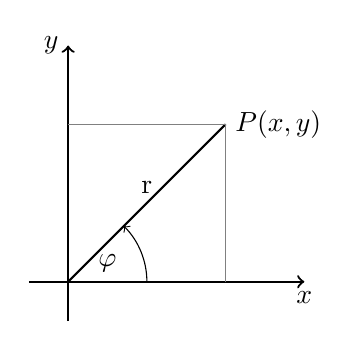
\begin{tikzpicture}
\draw [->,thick] (-0.5,0) -- (3,0); \node [below] at (3,0) {$x$};
\draw [->,thick] (0,-0.5) -- (0,3); \node [left] at (0,3) {$y$};

\draw [thick] (0,0) -- (2,2); \node [right] at (2,2){$P(x,y)$};
\draw [->] (1,0) arc [radius=1, start angle=0, end angle=45]; \node [above] at (0.5,0){$\varphi$};
\node [above] at (1,1) {r};
\draw[help lines] (2,0) -- (2,2); \draw[help lines] (0,2) -- (2,2);

\end{tikzpicture}\\
$x,y$ \dots kartesische Koordinaten\\
$r,\varphi$ \dots Polarkoordinaten (analog Betrag und Argument einer Komplexen Zahl) $r\geq 0, \varphi \in \mathbb{R}$\\
Umrechnung: $x = \cos{\varphi}, y = r\sin{\varphi}$
\item Kurvendarstellung: \[r=r(\varphi), \varphi \in [\alpha,\beta]\]
Für jeden Winkel $\varphi \in [\alpha,\beta]$ die Strecke $r(\varphi)$ auf dem $\varphi$ entsprechenden Strahl von $0$ aus abtragen

\end{itemize}
\subparagraph{Bemerkungen}
\begin{itemize}
\item Übergang explizite kartesische Darstellung zu Polarkoordinaten
\[y=f(x), x \in [a,b] \curvearrowright x=t, y=f(t), t \in [a,b] \]
\item Übergang explizite Polarkoordinatendarstellung zu Polarkoordinaten (Parameter $\varphi$)
\[r=r(\varphi),\varphi \in [\alpha,\beta] \curvearrowright x=r(\varphi)\cos{\varphi}, y= r(\varphi) \sin{\varphi}\; \varphi \in [\alpha,\beta]\]

\end{itemize}

\end{enumerate}

\paragraph{Tangenten und Normalen ebener Kurven}
\begin{itemize}
\item Anstieg $y'$ einer in Parameterdarstellung gegebenen Kurve $x=x(t)$, $y=y(t), t \in I$. Es sei $y=f(x)$ sei die explizite kartesische Darstellung (ohne die Elimination von $t$ tatsächlich auszuführen)\\
$\curvearrowright \frac{dy}{dt} = \frac{dy}{dx} \cdot \frac{dx}{dt}$ (Kettenregel). In Anwendungen ist $t$ oft die Zeit, übliche Schreibweise dann $\frac{dx}{dt} =: \dot{x}$,\\
$\frac{dy}{dt} =: \dot{y}$, also gilt $y'=\frac{\dot{y}}{\dot{x}}$\\
Höhere Ableitungen $\frac{d^2x}{dt^2} = \dot{\dot{x}}$ usw.
\item Tangente im Punkt $(x_0,y_0),y_0 = f(x_0) \text{ bzw. } x_0 = x(t_0), y_0 = y(t_0)$

Beispielvektor für Tangente $t=\begin{pmatrix} \dot{x} (t_0) \\ \dot{y} (t_0) \\ \end{pmatrix} =: \vec{\dot{r}} (t_0)$\\
Für $\vec{n} = \vec{n} (t_0) := \begin{pmatrix} -\dot{y}(t_0)\\ \dot{x} (t_0)\\ \end{pmatrix}$ gilt $(\vec{t},\vec{n}) = 0 \curvearrowright \vec{n} \perp \vec{t}$, damit ist $\vec{n}$ ein Richtungsvektor der Normalen
\end{itemize}

Tabelle 1 (Anstieg, Tangenten- und Normalenvektor):\\
$\begin{array}{c|c|c}
\text{Kurve} & y=f(x), x \in I & x = x(t), y= y(t), t \in I\\  \hline
\text{Punkt } P_0(x_0,y_0) & P_0(x_0,\underbrace{f(x_0)}_{y_0}) & P_0(x(t_0),y(t_0))\\ \hline
\text{Anstieg } m=\tan{\alpha} \text{ im Punkt } P_0 & f'(x_0) & \frac{\dot{y}(t_0)}{\dot{x} (t_0)} \\  \hline
\text{Tangentenvektor } \vec{t} & \begin{pmatrix} 1 \\ f'(x_0) \\ \end{pmatrix} & \begin{pmatrix} \dot{x} (t_0) \\ \dot{y} (t_0)\\ \end{pmatrix} \\  \hline
\text{Normalenvektor } \vec{n} & \begin{pmatrix} -f'(x_0) \\ 1\\ \end{pmatrix} & \begin{pmatrix} - \dot{y} (t_0) \\ \dot{x} (t_0) \\ \end{pmatrix}\\
\end{array}$

\begin{itemize}
\item Tangetengleichung
\[ y=y_0 + m \cdot (x-x_0) \quad \vec{r} = \begin{pmatrix} x \\ y \end{pmatrix} = \begin{pmatrix} x_0 \\ y_0 \\ \end{pmatrix} + s \cdot \vec{t}, s \in \mathbb{R} \]
\item Normalengleichung
\[ y = y_0 - \frac{1}{m} \cdot (x-x_0) \quad \vec{r} = \begin{pmatrix} x \\ y \end{pmatrix} = \begin{pmatrix} x_0 \\ y_0 \\ \end{pmatrix} + u \cdot \vec{n}, u \in \mathbb{R} \]
\end{itemize}

\paragraph{Krümmung ebener Kurven}
Gegeben sei Kurve $C$, fester Punkt $P_0 (x_0,y_0)$. $R$ und $S$ seien zwei weitere Punkte in $C$. Durch 3 Punkte $P_0,R,S$ ist im Allgemeinen eindeutig ein Kreis festgelegt. Es sei $K$ die Grenzlage des Kreieses, wenn $R$ und $S$ un $P_0$ übergehen.\\
\begin{itemize}
\item $K$ \dots Krümmungskreis
\item $\varkappa$ \dots Krümmung, vorzeichenbehaftet
\item $\varrho$ \dots Krümmungsradius $\varrho = \frac{1}{\lvert \varkappa \rvert}$
\item $M$ \dots Mittelpunkt von $K \;  \overrightarrow{0M} = \begin{pmatrix} x_0 \\ y_0 \end{pmatrix} + \frac{1}{\varkappa} \cdot \frac{\vec{n}}{\lvert \vec{n} \rvert}$
\end{itemize}

Tabelle 2\\
$\begin{array}{l|c|c|c}
\text{Kurve} & y=f(x), x \in I & \begin{array}{c} x = x(t)\\ y = y(t) \\ \end{array} , t \in I & r = r(\varphi), \varphi \in I\\ \hline
\text{Krümmung } \varkappa \text{ in } P(x,y) & \varkappa = \frac{y''}{(1+(y')^2)^{\frac{3}{2}}} & \varkappa = \frac{\dot{x} \dot{\dot{y}} - \dot{\dot{x}} \dot{y}}{(\dot{x}^2 + \dot{y}^2)^{\frac{3}{2}}} & \varkappa = \frac{r^2 + 2(r')^2 - rr''}{(r^2+(r')^2)^{\frac{3}{2}}} \\
\end{array}$

\paragraph{Raumkurven}
\begin{itemize}
\item Parameterdarstellung $\begin{array}{c} x=x(t)\\ y= y(t) z = z(t)\\ \end{array} t \in I$ vektoriell $\vec{r} = \vec{r} (t) = \begin{pmatrix} x(t) \\ y(t) \\ z(t) \\ \end{pmatrix}, t \in I$ mit $\vec{r} = \vec{r} = \begin{pmatrix} x \\ y \\ z \\ \end{pmatrix}$
\item Tangente in Punkt $P_0 (x(t_0),y(t_0),z(t_0))$
\[ \vec{r} = \vec{r} (t_0) + s \cdot \vec{\dot{r}}, s \in \mathbb{R}\]
\item Krümmung
\[ \varkappa = \frac{\lvert \vec{\dot{r}} \times \vec{\dot{\dot{r}}} \rvert}{\lvert \vec{\dot{r}} \rvert^3}, \text{ Radius } \varrho = \frac{1}{\varkappa} \]
\end{itemize}

\subsubsection{\textsc{Newton}-Verfahren zur Nullstellenermittlung}
\subparagraph{Satz 6} (\textsc{Newton}sches Iterationsverfahren)
Es sei $x^*$ eine Lösung der Gleichung $f(x) = 0$ für ein geeignetes Intervall $I=(x^*-r,x^*+r)$ gelte $f'(x) \neq 0 \wedge \lvert \frac{f(x) \cdot f''(x)}{(f'(x))^2} \rvert \leq k < 1 \; (x \in I)$\\
Dann konvergiert für jeden Startwert $x_0 \in I$ die mittels $x_{n+1} = x_n - \frac{f(x_n)}{f'(x_n)} \quad (n=0,1,2,\dots)$ festgelegte Folge gegen $x^*$. $\lim\limits_{n \to \infty} x_n = x^*$\\
Ferner gilt:
\[\lvert x^* -x_n \rvert \leq  \frac{K}{1-K} \lvert x_{n-1} - x_n \rvert \leq \frac{K^n}{1-K} \lvert x_1 - x_0 \rvert \]

\subparagraph{Diskussion}
\begin{enumerate}
\item Geometrische Veranschaulichung
\begin{itemize}
\item Tangente in $P_0$\\
$y = f(x_0) + f'(x_0) \cdot (x - x_0)$
\item $x_1$ \dots Nullstelle der Tangente\\
$0 = f(x_0) + f'(x_0) \cdot (x_1 - x_0)$\\
$\curvearrowright x_1 = x_0 - \frac{f(x_0)}{f'(x_0)}$
\end{itemize}
\item Zur Wahl des Startwertes $x_0$:\\
Falls in $I$ gilt $f''(x) \begin{array}{c} > \\ < \\ \end{array} 0$, dann günstig für Startwert: $f (x_0) \begin{array}{c} > \\ < \\ \end{array} 0$
\item Praktisches Vorgehen: Abbruch falls $\lvert x_{n+1} - x_n \rvert < \varepsilon$
\end{enumerate}

\section{Integralrechnung für Funktionen einer reellen Veränderlichen}
\subsection{Integralbegriff}
\subsubsection{Das bestimmte Integral}
\subparagraph{Problem} Geg: Kurve $y=f(x), \; x \in [a,b]$ (zunächst $f(x) \geq 0$)\\
Ges: Flächeninhalt $I$ unter der Kurve.
\subparagraph{Vorgehensweise}
\begin{itemize}
\item Zerlegung $Z$ des Intervalls $[a,b] \cdot a = x_0 < x_1 < x_2 < \dots < x_{n-1} < x_n = b$
\item In jedem Teilintervall Zwischenstelle $\xi \in [x_{i-1}, x_i]$ wählen $\curvearrowright$ Zerlegung $Z^*$ ($Z$ mit Zwischenstellen $\xi_i$)
\item $\Delta (Z^*) := \max{(x_i - x_{i-1} )}_{i = 1,\dots,n} $ \dots max. Teilintervalllänge
\item Approximation von $I$ durch Summe von Rechtecksflächen:
\[ S(Z^*,f) := \sum\limits_{i=1}^{n} f(\xi_i) \cdot (x_i - x_{i-1} )\]
\dots sogenannte \textsc{Riemann}sche Summe (Näherung für $I$)
\end{itemize}
\subparagraph{Definition 1} Die Funktion $f$ heißt (im \textsc{Riemann}schen Sinne) über $[a,b]$ integrierbar, wenn für jede Zerlegungsfolge $ \forall (Z^*\mu)$ von $[a,b]$ mit $\lim\limits_{\mu \to \infty} \Delta (Z_\mu^*) = 0$ gilt. $\lim\limits_{\mu \to \infty} S(Z_\mu^*,f) = I$\\
Die Zahl $I$ heißt bestimmtes Integral von $f$ über $[a,b]$\\
Bezeichnung $I = \int\limits_{a}^{b} f(x) \,dx$

\subparagraph{Diskussion}
\begin{enumerate}
\item Definition 1 basiert nicht auf der Forderung $f(x) \geq 0$. Falls $f(x) < 0 \text{ für } x \in [a,b]$, so gilt im Falle der Integrierbarkeit: $\int\limits_{a}^{b} f(x) \, dx <0$ 
\item Man definiert: $\int\limits_{a}^{a} f(x) \, dx := 0, \int\limits_b^* f(x) \, dx, \; b > a$
\item Eigenschaften des bestimmten Integrals
$\int\limits_a^b f(x) \, dx =  \int\limits_a^c f(x) \, dx  + \int\limits_c^b f(x) \, dx \quad (a,b,c \in \mathbb{R} ) $
\[ \int\limits_a^b (c_1 u(x) + c_2 v(x)) \, dx = c_1 \int\limits_a^b u(x) \, dx + c_2 \int\limits_a^b v(x) \, dx \]
\end{enumerate}

\subparagraph{Satz 1} Es sei $f(x)$ stetig in $[a,b]$. Dann ist $f(x)$ über $[a,b]$ integrierbar.

\subparagraph{Diskussion}
\begin{enumerate}
\item Falls $f(x)$ stückweise stetig ist mit endlichen vielen endlichen Sprungstellen, so ist $f$ ebenfalls integrierbar
\item Nicht integrierbar (im \textsc{Riemann}schen Sinne) ist z.B.
\[f(x) = \left\{ \begin{array}{lccr} 1 & \mbox{für} & x & \text{ irrational}\\ 0 & \mbox{für} & x & \text{ rational} \\ \end{array} \right. , x \in [0,1] \]
\end{enumerate}

\subsubsection{Stammfunktionen, unbestimmtes Integral}
\subparagraph{Satz 2}(Mittelwertsatz der Integralrechnung)\\
$f$ sei auf $[a,b]$ stetig $\Rightarrow \exists \xi \in (a;b]: \int\limits_a^b f(x) \, dx = f(\xi) \cdot (b-a)$\\
$m = \frac{1}{b-a} \int\limits_a^b f(x) \, dx$ \dots (Integral)- Mittelwert von $f$ über $[a,b]$\\
Integrale mit variabler oberer Grenze\\
\[ \int\limits_a^x f(t) \, dt =: F(x) \]

\subparagraph{Satz 3} $f$ stetig auf $[a,b] \Rightarrow F(x) = \int\limits_a^x f(t) \, dt, \; x \in [a,b]$ ist auf $[a,b]$ differenzierbar, und es gilt $F'(x) = f(x)$

Beweis: $\frac{F(x+h) - F(x)}{h} = \frac{\int\limits_{x}^{x+h} f(t) \, dt}{h} = \frac{h \cdot f(\xi)}{h} \underbrace{=}_{\text{Satz 2}, \xi \in [x,x+h]} f(\xi) \Leftarrow_{h \to 0} f(x)$
$\underline{\underline{F'(x) = f(x)}}$

\subparagraph{Definition 2} Die Funktion $F(x)$ heißt Stammfunktion von $f(x)$ (auf $[a,b]$), wenn gilt $F'(x) = f(x)$.
\subparagraph{Diskussion} Ist $F(x)$ eine Stammfunktion, so ist auch $F(x) + c$ ($c \in \mathbb{R}$, konstant) eine Stammfunktion.
\subparagraph{Definition 3} Die Menge aller Stammfunktionen von $f$, d.h. $\{ F(x) +c | c \in \mathbb{R} \}$, wobei $F(x)$ eine beliebige Stammfunktion von $f$ ist, heißt unbestimmtes Integral von $f$ :\\
Bezeichnung $\int f(x) \, dx = F(x) +c $

\subsubsection{Hauptsatz der Differential- und Integralrechnung}
\subparagraph{Satz 4} $f$ sei stetig auf $[a,b], F(x)$ \dots bel. Stammfunktion $\Rightarrow \int\limits_a^b f(x) \, dx = F(b) - F(a)$\\
Schreibweise: $[ F(x)]_a^b := F(b) - F(a)$

Beweis: Satz 3, $F_1(x) := \int\limits_a^x f(t) \, dt$ ist Stammfunktion von $f$, also gilt $F(x) = F_1(x) + k$\\
$\curvearrowright F(b) - F(a) = (F_1(b) + k) - (F_1(a) +k) = F_1(b) - \underbrace{F_1(a)}_{0} = F_1(b) = \int\limits_a^b f(t) \, dt = \int\limits_a^b f(x) \, dx$

\subparagraph{Diskussion}
\begin{enumerate}
\item \begin{tabular}{p{5cm}p{1cm}p{5cm}} $\int\limits_a^b f(x) \, dx$ & $ =$ & $ F(b) - F(a)$ \\
Flächeninhaltsproblem (\underline{\underline{Integralrechnung}}) && Stammfunktion, Umkehrung der \underline{\underline{Differentialrechnung}}\\ \end{tabular}
\item Symbolik $\frac{dF(x)}{dx} = f(x) \Leftrightarrow \underbrace{\int dF(x)}_{F(x)+c} = \int f(x) \, dx$
\item Differential Tabelle: Tabelle unbestimmter Grundintegrale\\
Beispiele:
\begin{enumerate}
\item $\frac{d}{dx} \cos{x} = - \sin{x} \Leftrightarrow \int (-\sin{x}) \, dx = \cos{x} + c^* \; | \cdot (-1)$\\
$\int\sin{x} \, dx = - \cos{x} +c$ (mit $c = -c^*$)
\item $\frac{d}{dx} x^{\alpha +1} = (\alpha +1 ) x^\alpha \Leftrightarrow \int (\alpha +1) x^\alpha \, dx = x^{\alpha +1} + c^* \; | \cdot \frac{1}{\alpha +1}$\\ $  \Leftrightarrow \int x^\alpha \, dx = \frac{x^{\alpha +1}}{\alpha +1} +c, \alpha \neq -1$
\end{enumerate}

\end{enumerate}

\subsection{Integrationsmethoden}
\subsubsection{Substitution}
Zu berechnen sei $\int f (g(x)) \cdot g'(x) \, dx$. Bekannt sei eine Stammfunktion $F(x)$ von $f(x)$.\\
Lösung: Substitution $u=g(x) \curvearrowright \frac{du}{dx} = g'(x) \curvearrowright du = g'(x) \, dx$

\begin{equation}\label{421Sbst1}
\int f(g(x)) g'(x) \, dx = \int f(u) \, du = F(u) +c \underbrace{=}_{\text{Rücksubst.}} F(g(x)) + c
\end{equation}

Merke: Anwendung zweckmäßig, wenn der Integrand das Produkt einer mittelbaren Funktion und der Ableitung der inneren Funktion ist, und außerdem eine Stammfunktion der äußeren Funktion bekannt ist.

\subparagraph{Beispiel 1} $\int \frac{1}{x} \cdot \sqrt[3]{\ln{x}} \, dx \underbrace{=}_{u = \ln{x}; \frac{du}{dx} = \frac{1}{x} \curvearrowright du=\frac{1}{x} dx} = \int \sqrt[3]{u} \, du = \frac{3}{4} u^{\frac{4}{3}} + c = \frac{3}{4} ( \ln{x})^{\frac{4}{3}} +c$

\subparagraph{Beispiel 2} $\int x e^{-x^2} \, dx \underbrace{=}_{u = -x^2, \frac{du}{dx} = -2x, \curvearrowright dx =- \frac{du}{2x}} \int e^u \cdot (-\frac{du}{2}) = -\frac{1}{2} \int e^u \, du = -\frac{1}{2} e^u +c = -\frac{1}{2} e^{-x^2} +c$

\subparagraph{Beispiel 3} (Substitution bei bestimmten Integralen)
\begin{enumerate}
\item Möglichkeit: Grenzen mit Substituieren: $x=0 \curvearrowright u = 1, x= \sqrt{8} \curvearrowright u = 9$\\
 $I = \int\limits_{x=0}^{\sqrt{8}} x \cdot \sqrt{1 +x^2} \, dx \underbrace{=}_{u=1+x^2, \frac{du}{dx} = 2x, dx= \frac{du}{2x}} \int\limits_{u=1}^{9} \sqrt{u} \frac{du}{2} = \frac{1}{2} \cdot \frac{2}{3} [ u ^{\frac{3}{2}}]^9_{u=1} = \frac{1}{3} (27-1) = \frac{26}{3}$
\item Möglichkeit: Unbestimmte Integration (mit Rücksubstituion) anschließend $x$-Grenzen einsetzten\\
$\int x \sqrt{1+x^2} \, dx = \frac{1}{3} (1+x^2)^{frac{3}{2}} + c$\\
$I = [ \frac{1}{3} (1+x^2)^{\frac{3}{2}} ]_{x=0}^{\sqrt{8}} = \frac{26}{3}$
\end{enumerate}

\subparagraph{Beispiel 4}(Lineare Substitution)\\
Allgemein: $\int f(ax+b) \, dx \underbrace{=}_{u = ax+b, \frac{du}{dx} = a, dx= \frac{du}{a}} \int f(u) \frac{du}{d} = \frac{1}{a} F(u) +c = \frac{1}{a} F(ax+b) +c$

\begin{enumerate}
\item $\int \cos{(3x)} \, dx = \frac{1}{3} \sin{(3x)} + c$
\item $\int e^{-2x} \, dx = - \frac{1}{2} e^{-2x} +c$
\item $\int (3x -4)^6 \, dx  = \frac{1}{3} \cdot \frac{1}{7} (3x-4)^7 +c = \frac{1}{21} (3x-4)^7 +c$
\item $\int \sin{(\frac{x}{2} + \pi )} \, dx = \frac{1}{\frac{1}{2}} \cdot (-\cos{(\frac{x}{2} + \pi)})+c = -2\cos{(\frac{x}{2} + \pi)} +c$
\end{enumerate}

\subparagraph{Diskusison} Neben diesen "`natürlichen"', leicht(?!) [!sic] erkennbaren Substitutionen sind weitere denkbar durch Einführung "`künstlicher"' Variabler
\begin{equation}\label{421_1'}
\int f(x) \, dx \underbrace{=}_{x= \varphi (t), \frac{dx}{dt} = \varphi' (t) \curvearrowright dx = \varphi' (t) \,dt} \int f(\varphi (t)) \varphi' (t) \, dt
\end{equation}

(\ref{421_1'}) entspricht (\ref{421Sbst1}) von rechts nach links gelesen. Falls rechte Seite von (\ref{421_1'}) integrierbar (Stammfunktion $H(t)$), dann 
\[ \int f(x) \, dx = H(t) +c = H(\varphi^{-1} (x)) +c \]
(Vorraussetzung: $\varphi^{-1}$ existiert)

\subparagraph{Beispiel 5} $\int \frac{1}{\sqrt{1+x^2}} \, dx \underbrace{=}_{ x= \text{sinh}\, t \curvearrowright \sqrt{1+x^2} = \text{cosh}\, t, \frac{dx}{dt} = \text{cosh}\, t \curvearrowright dx = \text{cosh} \, dt} \int \frac{1}{\text{cosh}\, t} \, dt = \int dt = t+c = \text{arcsinh}\, x + c = \ln{(x+\sqrt{x^2+1})} +c$

\subparagraph{Beispiel 6} $\int \frac{f'(x)}{f(x)} \, dx = \ln{\lvert f(x) \rvert} +c$ (Zähler = 1. Abbleitung des Nenners)\\
(denn : $u=f(x) \curvearrowright \frac{du}{dx} = f'(x) \curvearrowright du= f'(x) \, dx \curvearrowright \int \dots = \int \frac{1}{u} \cdot du = \ln{\lvert u \rvert} + c = \ln{\lvert f(x)\rvert} +c$

\subsubsection{Partielle Integration}
Produktregel der Differentialrechnung\\
$\frac{d}{dx} (u(x) \cdot v(x)) = u'(x) \cdot v(x) + u(x) \cdot v'(x)$\\
$u(x) \cdot v(x) = \int u'(x) \cdot v(x) \, dx + \int u(x) v'(x) \, dx$
\[\curvearrowright \int u(x) \cdot v'(x) \, dx = u(x) \cdot v(x) - \int u'(x) \cdot v(x) \, dx\]
(partielle Integration)

\subparagraph{Beispiel 8} $\int \arctan{x} \, dx = x \cdot \arctan{x} - \frac{1}{2} \int \frac{2x}{1+x^2} \, dx$\\
$\begin{array}{|c|c|}\hline
u=\arctan{x} & u'= \frac{1}{1+x^2} \\ \hline
v'=1 & v=x \\ \hline
\end{array}$\\
$= x \arctan{x} - \frac{1}{2} \ln{\lvert 1 + x^2 \rvert} + c$\\
$\underline{\underline{= x \arctan{x} - \frac{1}{2} \ln{(1+x^2)}+c}}$

\subsubsection{Integration gebrochenrationaler Funktionen}
\begin{itemize}
\item Geg.: Gebrochen rationale Funktion: $f(x) = \frac{p(x)}{q(x)}$
\item Integration erfolgt in den Schritten 1.-5.
\end{itemize}
\begin{enumerate}
\item Falls $f$ unecht gebrochen: Polynomdivision
\[f(x) = \underbrace{a(x)}_{\text{Polynom}} + \underbrace{\frac{r(x)}{q(x)}}_{\text{echt gebrochen}} \quad | r(x) \dots \text{ Rest} \]
\item Nullstellen des Nenners $q(x)$ ermitteln
Zerlegung \begin{equation}\label{4231} q(x) = (x-\alpha_1)^{k_1} \cdot (x-\alpha_2)^{k_2} \cdot \dots \cdot (x^2 + p_1 x + q_1)^{m_1} \cdot \dots \end{equation}
($\alpha_n$ \dots reelle Nullstellen, $p_n$ \dots reell nicht zerlegbar)\\
Eventuell gemeinsame Faktoren in $r(x)$ und $q(x)$ kürzen!
\item Ansatz für die sogenannte Partialbruchzerlegung (PZ)
\[\frac{r(x)}{q(x)} = \text{Summe von Partialbrüchen}\]
Jedem Faktor $\left\{ \begin{array}{c} (x-\alpha)^k \\ (x^2 + px +q)^m \\ \end{array} \right.$ aus (\ref{4231}) entspricht\\ der Anteil $\left\{ \begin{array}{c}
\frac{A_1}{x-\alpha} + \frac{A_2}{(x-\alpha)^2} + \dots + \frac{A_k}{(x-\alpha)^k} \\
\frac{B_1x + c_1}{x^2 +px +q} + \dots + \frac{B_mx + c_m}{(x^2 + px + q)^m} \\
\end{array}\right.$
in dieser Summe.

\subparagraph{Beispiel 9} $f(x) = \frac{x^2+4}{(x-1)^3 \cdot (x+5) \cdot (x^2 + 2x + 2)^2}$\\
Ansatz für PZ:
\[f(x) = \frac{A}{x-1} + \frac{B}{(x-1)^2} + \frac{C}{(x-1)^3} + \frac{D}{x+5} + \underbrace{ \frac{Ex+F}{x^2+2x+2} + \frac{Gx+H}{(x^2 + 2x +2)^2}}_{(x^2 +2x +2 \text{ ist reell nicht zerlegbar, Nullstellen sind } -1\pm i)}\]

\item Ermittlung der Koeffizienten durch
\begin{enumerate}
\item Multiplikation des Ansatzes für PZ mit Nenner $q(x)$
\item Kombination der beiden folgenden Methoden
\begin{enumerate}
\item Einsetzten der reellen Nullstellen (Falls alle Nullstellen reell und einfach sind, können damit alle Koeffizienten bestimmt werden)
\item Restliche Koeffizienten durch Koeffizientenvergleich bestimmen!
\end{enumerate}
(vgl. Beispiele)
\end{enumerate}
\item Interpretation der Partialbrüche
\begin{enumerate}
\item $\int \frac{1}{(x-\alpha)^j} \, dx = \left\{ \begin{array}{lr}
\ln{\lvert x - \alpha \rvert } + c & (j=1)\\
\frac{1}{1-j} \cdot (x-\alpha)^{1-j} + c & (j=2,3,\dots)\\ \end{array} \right.$
\item $\int \frac{Bx+c}{(x^2 + px +q)^j} \, dx \underbrace{=}_{\text{Zerlegung}} \int ( \frac{\frac{B}{2} (2x + p) }{(x^2 + px +q)^j} + \frac{c- \frac{B}{2} p}{(x^2 + px +q)^j} ) \, dx$
\begin{enumerate}
\item $\int \frac{ 2x+p}{(x^2 + px +q)^j} \, dx:$ Substitution $x^2+px+q=u$\\ $du=(2x+p) \, dx$ usw.
\item $\int \frac{dx}{(x^2 + px +q)^j} = \int \frac{dx}{((x + \frac{p}{2})^2 + q- \frac{p^2}{4} )^j} = \int \frac{du}{(u^2 + a^2 )^j}$\\
(mit $a^2 := q - \frac{p^2}{4} > 0$ und $ u = x + \frac{p}{2}, du=dx$)\\
$j=1$: vgl. Merkblatt\\
$j > 1$: s geeignete Formelsammlung
\end{enumerate}
\end{enumerate}
\end{enumerate}

\subparagraph{Beispiel 10} $I = \int \frac{3x+4}{x^2+2x-3} \, dx$
\begin{itemize}
\item Echt gebrochen, Nullstellen des Nenners $x_1 = -3, x_2 = 1$\\
Zerlegung: $q(x) = x^2 +2x -3 = (x+3)(x-1)$
\item Ansatz für PZ: $\frac{3x+4}{(x+3)(x-1)} = \frac{A}{x+3} + \frac{B}{x-1} \quad | \cdot \underbrace{(x+3)+(x-1)}_{q(x)}$\\
$3x+4 = A \cdot (x-1) + B(x+3)$\\
Einsetzen $x=-3: -5 = A (-4) \curvearrowright \underline{\underline{A= \frac{5}{4}}}$\\
$x= 1: 7 = B \cdot 4 \curvearrowright \underline{\underline{ B = \frac{7}{4}}}$\\
$I = \int (\frac{\frac{5}{4}}{x+3} + \frac{\frac{7}{4}}{x-1} ) \, dx = \underline{\underline{\frac{5}{4} \ln{\lvert x + 3 \rvert} + \frac{7}{4} \ln{\lvert x -1 \rvert} +c}}$

\end{itemize}

\subsubsection{Integration von Potenzreihen}
\subparagraph{Satz 1} Es sei 
\[ f(x) = \sum\limits_{n=0}^{\infty} a_n(x-x_0)^n, x \in ( x_0 -r , x_0 +r)\]
\[ \Rightarrow F(x) = \sum\limits_{n=0}^{\infty} \frac{a_n}{n+1} (x - x_0)^{n+1}, x \in (x_0 -r, x_0 + r )\] ist Stammfunktion von $f(x)$. (gliedweise Integration)

\subparagraph{Beispiel 12}
\[ \arctan{x} = x - \frac{x^3}{3} + \frac{x^5}{5} - \frac{x^7}{7} \pm \dots \quad (\lvert x \rvert < 1)\]
Folgerung: $x=1 \curvearrowright \underbrace{\frac{\pi}{4}}_{\arctan{1}} = 1 - \frac{1}{3} + \frac{1}{5} - \frac{1}{7} + \dots$

\subparagraph{Beispiel 13} Gesucht Stammfunktion $F(x)$ zu $f(x) = e^{-x^2}$\\
$[ ! e^x = 1 + x + \frac{x^2}{2!} + \frac{x^3}{3!} + \dots ]$\\
$\int\limits_{0}^x e^{-t^2} \, dt = \int\limits_0^x (1-t^2 + \frac{t^4}{2!} - \frac{t^6}{3!} \pm \dots) \, dt = x-\frac{x^3}{3} + \frac{x^5}{5\cdot 2!} - \frac{x^7}{7\cdot 3!} + \frac{x^9}{9 \cdot 4!} \pm \dots = F(x) \quad (x \in \mathbb{R}$

\subparagraph{Diskussion}
\begin{enumerate}
\item $\int e^{-x^2} \, dx$ ist nicht in geschlossener Form darstellbar.
\item Für nicht zu große $x$: Reihendarstellung zur Berechnung von $\int\limits_0^x e^{-t^2} \, dt$ gut geeignet: z.B. gilt:
\begin{itemize}
\item $I=\int\limits_0^1 e^{-x^2} \, dx = 1 -\frac{1}{3} + \frac{1}{5\cdot 2!} - \frac{1}{7\cdot 3!}  \pm \dots + \frac{1}{17\cdot 8!} \pm \dots \approx 0,74682427 $
\item $\lvert \text{Fehler} \rvert \leq \frac{1}{19\cdot 9!} = 1,4504 \cdot 10^-7$ (vgl. \textsc{Leibnitz}-Kriterium,2.1.3.)\\
$\underline{\underline{I = 0,746824}} \quad (b$ Stellen genau)
\end{itemize}
\end{enumerate}

\subsection{Numerische Integration}
\subparagraph{Ziel} Berechnung ovn $\int\limits_a^b f(x) \, dx$ falls Stammfunktion nicht in geschlossener Form darstellbar.
\subparagraph{Prinzip}
\begin{enumerate}
\item Zerlegung von $[a,b]$ in $n$ gleichlange Teilintervalle der Länge $h= \frac{1}{n} (b-q)$\\
$\curvearrowright \text{ Teilpunkte } x_k = a + k\cdot h (k=0,1,\dots,n), y_k = f(x_k)$
\item Ersetzen von $f(x)$ über den Teilintervallen durch einfachere Funktionen, z.B. lineare Funktionen (Trapezregel), quadratische Funktionen (\textsc{Simpson}-Regel)\\
Näherung für I:
\begin{equation}\label{431}I \approx S_n(h) = \frac{h}{3} ((y_0 + y_n ) +4(y_1+y_3+\dots + y_{n-1}) + 2(y_2 +y_4 + \dots + y_{n-2}))\end{equation}
($n$ gerade)

\end{enumerate}


\subparagraph{Diskussion}
\begin{enumerate}
\item Fehlerabschätzung
\[ I = S_n (h) - \frac{h^4 (b-a)}{180} \cdot f^{(4)} (\xi), \quad a < \xi < b\]
(falls $f^{(4)}$ stetig auf $[a,b]$)
\item \textsc{Simpson}-Regel ist für Polynome bis einschließlich 3. Grades exakt.
\item Praktische Durchführung: Schrittweitenhalbierung.\\
Startwert $S^{(1)} := S_n(h)$ für geeignetes $n$ (z.B: $n=4$).\\
$S^{(2)} = S_{2n} (\frac{h}{2}), S^{(3)} = S_{4n} (\frac{h}{4})$ usw., bis sich die Ziffern im Rahmen der gewünschten Genauigkeit nicht mehr ändern.
\end{enumerate}

\subparagraph{Beispiel 1} $I = \int\limits_0^1 e^{-x^2} \, dx$
\begin{itemize}
\item $n= 4, h=0,25$\\
$\begin{array}{c|c|c|c|c}
k & x_k & y_0,y_n & y_{2_{j+1}} & y_{2_j}\\ \hline
0 & 0 & 1,000000 & \\
1 & 0,25 & & 0,939413 \\
2 & 0,5 & & &0,778801\\
3 & 0,75 & & 0,569783 \\
4 & 1,0 & 0,367879 &  \\ \hline
 & & 1,367879 & 1,509196 & 0,778801\\
\end{array}$

(\ref{431}) $\curvearrowright S_4(0,25) = \frac{0,25}{3} (\dots + 4 \cdot \dots + 2 \cdot \dots) = 0,746855$

\item Schrittwertenhalbierung
$\begin{array}{c|c|c}
n & h & S_n(h)\\ \hline
4 & 0,25 & 0,746855\\
8 & 0,125 & 0,746826\\
16 & \dots & 0,746824 \\
32 & \dots & 0,746824\\
\end{array}$
$\curvearrowright I = 0,746824$ (vgl. Beispiel 13, Kapitel 4.2.)
\end{itemize}

\subsection{Uneigentliche Integrale}
\begin{itemize}
\item Vorbetrachtung\\
Bisher $\int\limits_a^b f(x) \, dx$ (endliches Intervall $[a,b]$, stückweise stetig und damit beschränkte Funktion $f$
\item 2 Erweiterungen
\begin{enumerate}
\item Unendliches Intervall $[a;\infty), (-\infty;b]$ bzw. $(-\infty;\infty)$
\item Unbeschränkte Funktionen (Polstellen)
\end{enumerate}
\item Vorgehensweise: "`Herausschneiden"' der kritischen Stelle(n), anschließend Grenzübergang
\begin{enumerate}
\item Unendliches Intervall
\begin{enumerate}
\item $\int\limits_{-\infty}^b f(x) \, dx := \lim\limits_{A \to - \infty} \int\limits_{A}^{b} f(x) \, dx$\\
analog $\int\limits_a^\infty f(x) \, dx := \lim\limits_{B \to \infty} \int\limits_a^B f(x) \, dx$
\item $\int\limits_{-\infty}^{\infty} f(x) \, dx := \lim\limits_{\begin{array}{c}A\to - \infty \\ B \to \infty \end{array}} \int\limits_A^B f(x) \, dx$
\end{enumerate}
\end{enumerate}

\end{itemize}

\subparagraph{Diskussion}
\begin{enumerate}
\item Falls Grenzwerte existieren, Sprechweise: Integral is konvergent, sonst divergent
\item Vorkommen z.B: \[\Gamma (x) = \int\limits_0^\infty e^{-t} t^{x-1} \, dt \quad (x > 0)\]
(Gamma Funktion) Eigenschaft: $\Gamma (n) = (n-1)!$ für $n\in \mathbb{N}^*$


\subparagraph{Beispiel 1}
\begin{itemize}
\item $\int\limits_0^\infty e^{-x} \, dx = \lim\limits_{A \to \infty} \int\limits_0^A e^{-x} \, dx = \lim\limits_{A \to \infty} [-e^{-x}]_0^A = \lim\limits_{A \to \infty} (-e^{-A} +1 ) = \underline{\underline{1}}$
\item $\int\limits_0^\infty \cos{x} \, dx = \lim\limits_{A \to \infty} \int\limits_{0}^A \cos{x} \, dx = \lim\limits_{A \to \infty} [\sin{x}]_0^A  = \lim\limits_{A \to \infty} \sin{A} \curvearrowright$ existiert nicht (unbestimmt divergent)
\item $\int\limits_1^\infty \frac{1}{x} \, dx = \lim\limits_{A \to \infty} \int\limits_1^A \frac{1}{x} \, dx = \lim\limits_{A \to \infty} [\ln{\lvert x \rvert}]_1^A = \lim\limits_{A \to \infty} \ln{A} = \underline{\underline{\infty}}$ (bestimmt divergent)
\end{itemize}

\item Unbeschränkter Integrand
\begin{enumerate}
\item Z.B: Unendlichkeitsstelle bei $b$
\[ \int\limits_a^b f(x) \, dx := \lim\limits_{\varepsilon \to + 0} \int\limits_{a}^{b-\varepsilon} f(x) dx\]
\item Unendlichkeitsstelle $x_0 \in (a;b)$ (Im Inneren)
\[ \int\limits_a^b f(x) \, dx = \lim\limits_{\delta \to + 0} \int\limits_{a}^{x_0 - \delta} f(x) \, dx + \lim\limits_{\varepsilon \to +0} \int\limits_{x_0 + \varepsilon}^b f(x) \, dx\]
\end{enumerate}
\subparagraph{Beispiel 2} $\int\limits_0^4 \frac{1}{\sqrt{x}} \, dx = \lim\limits_{\varepsilon \to +0} \int\limits_\varepsilon^4 \, dx = \lim\limits_{\varepsilon \to + 0} [2 \sqrt{x} ]_\varepsilon^4 = \underline{\underline{4}} $

\item Unendliches Intervall und unendliche Funktion
\subparagraph{Beispiel 3} $I = \int\limits_{1}^{\infty} \frac{dx}{x \cdot \sqrt{x-1}}$\\
NR: $\int \frac{dx}{x \sqrt{x-1}} \underbrace{=}_{u = \sqrt{x-1} \leftrightarrow x = u^2 +1, \frac{dx}{du} = 2u} \int \frac{2u du}{(u^2 +1)u} = 2 \arctan{u} +c = 2 \arctan{\sqrt{x-1}} +c$\\
$I = \lim\limits_{\varepsilon \to +0; A \to \infty} \int\limits_{1+\varepsilon}^A \dots = \lim\limits_{\varepsilon \to +0; A \to \infty} [2 \arctan{\sqrt{x-1}}]^A_{1+\varepsilon} = \lim\limits_{A \to \infty} 2 \arctan{\sqrt{A-1}} - \lim\limits_{\varepsilon \to + 0}  2 \arctan{\sqrt{\varepsilon}} = \underline{\underline{\pi}}$
\end{enumerate}

\subsection{Anwendungen}
\subsubsection{Geometrische Anwendungen}
\paragraph{Inhalt ebener Flächenstücke}
\begin{itemize}
\item $y=f(x) \geq  0, \quad a<b$\\
\[ F=\int\limits_a^b f(x) \, dx\]
\item \[F= \int\limits_a^c \lvert f(x) \rvert \, dx = \lvert \int\limits_a^b f(x) \, dx \rvert + \lvert \int\limits_b^c  f(x) \, dx \rvert \]
\item \[ F= \int\limits_{x_1}^{x_2} (f(x) - g(x) ) \, dx\]
\end{itemize}

\subparagraph{Beispiel} Gesucht ist der Flächeninhalt $F$ des von der Ellipse $\frac{x^2}{a^2} + \frac{y^2}{b^2} = 1 \; (a >0, b>0)$ begrenzten Bereiches.
\begin{itemize}
\item Auflösen nach $y: \; y= \pm b \cdot \sqrt{1-\frac{x^2}{a^2}}$\\
$\underbrace{\curvearrowright}_{\text{Symmetrie}} F= 4 \cdot \int\limits_0^a b \cdot \sqrt{1-\frac{x^2}{a^2}} \, dx -= \frac{4b}{a} \int\limits_0^a \sqrt{a^2-x^2} \, dx \underbrace{=}_{(1)} \frac{4b}{a} \left [ \frac{1}{2} ( x \sqrt{a^2-x^2} + a^2 \arcsin{(\frac{x}{a})} ) \right ]_0^a$\\
$=\frac{4b}{a} \cdot \frac{1}{2} a^2 \underbrace{\arcsin{1}}_{\frac{\pi}{2}} = \underline{\underline{\pi a b}}$\\
(1) s Tabelle oder Substituiere $x= a \sin{t}, \sqrt{a^2-x^2} = a \cos{t} \; \frac{dx}{dt} = a \cos{t}$ usw.
\end{itemize}

\paragraph{Bogenlänge}
\subparagraph{Bogenlänge ebener Kurven} Kurve K mit P.d.\\
$x=x(t) \; y=y(t) \; \alpha \leq t \leq \beta$\\
\definecolor{qqqqff}{rgb}{0.0,0.0,1.0}
\begin{tikzpicture}[line cap=round,line join=round,>=triangle 45,x=1.0cm,y=1.0cm]
\draw[->,color=black] (-0.019919504841264316,0.0) -- (14.71960362224012,0.0);
\foreach \x in {,1.0,2.0,3.0,4.0,5.0,6.0,7.0,8.0,9.0,10.0,11.0,12.0,13.0,14.0}
\draw[shift={(\x,0)},color=black] (0pt,2pt) -- (0pt,-2pt) node[below] {\footnotesize $\x$};
\draw[->,color=black] (0.0,-2.636086465572875) -- (0.0,5.3594095703439155);
\foreach \y in {-2.0,-1.0,1.0,2.0,3.0,4.0,5.0}
\draw[shift={(0,\y)},color=black] (2pt,0pt) -- (-2pt,0pt) node[left] {\footnotesize $\y$};
\draw[color=black] (0pt,-10pt) node[right] {\footnotesize $0$};
\clip(-0.019919504841264316,-2.636086465572875) rectangle (14.71960362224012,5.3594095703439155);
\draw [shift={(8.279243955481641,-7.430657541256236)}] plot[domain=1.2460831447972658:2.2281480975538117,variable=\t]({1.0*11.913215108603938*cos(\t r)+-0.0*11.913215108603938*sin(\t r)},{0.0*11.913215108603938*cos(\t r)+1.0*11.913215108603938*sin(\t r)});
\draw (5.2362500631179465,3.5517322057018585) node[anchor=north west] {Kurve K};
\begin{scriptsize}
\draw [fill=qqqqff] (1.0,2.0) circle (1.5pt);
\draw[color=qqqqff] (1.120307755932956,2.230737208463432) node {$P_0$};
\draw [fill=qqqqff] (5.7,4.2) circle (1.5pt);
\draw[color=qqqqff] (5.820268904002303,4.4416656775256405) node {$P_1$};
\draw [fill=qqqqff] (12.08,3.86) circle (1.5pt);
\draw[color=qqqqff] (12.202760522238489,4.094035415094476) node {$P_n$};
\end{scriptsize}
\end{tikzpicture}

\begin{itemize}
\item Vorgehen: Approx. durch Streckenzug, Verfeinerung. Länge des Streckenzugs:
\[\sum\limits_{i=1}^n \overline{P_{i-1}P_j} = \sum\limits_{i=1}^n \sqrt{(\Delta x_i)^2 + ( \Delta y_i)^2} \underbrace{=}_{*} \sum\limits_{i=1}^n \sqrt{(\dot{x} (u_i))^2 + (\dot{y} (v_i))^2} \Delta t_i\] 
$*$) MWS der Diff-Rechnung, Zwischenstellen $u_i,v_i \in (t_{i-1},t_i)$

Verfeinerung: $\int\limits_\alpha^\beta  \sqrt{(\dot{x} (t))^2 + (\dot{y} (t))^2 } \, dt$

\item Diskussion
\begin{enumerate}
\item Bogenlänge der Kurve $\vec{r} = \vec{r}(t) = \begin{pmatrix} x(t) \\ y(t) \\ \end{pmatrix}$ zwischen $\alpha$ und $t$ ($t$ variabel)\\
$s= \int\limits_\alpha^t \underbrace{\sqrt{(\dot{x} (u))^2 + ( \dot{y} (u))^2}}_{\lvert \vec{\dot{r}} (u) \rvert}$\\
$\frac{ds}{dt} = \lvert \dot{\vec{r}} (t) \rvert \curvearrowright ds = \lvert \dot{\vec{r}} (t) \rvert \, dt = \sqrt{\dot{x}^2 + \dot{y}^2} \, dt$ \dots Bogenelement
\item Tabelle (Bogenlänge ebener Kurven)\\
$\begin{array}{c|c}
\text{Kurvendarstellung} & \text{Bogenlänge } s, \text{ Bogenelement } ds \\ \hline
x=x(t), y=y(t) , t \in [a;\beta] & s = \int\limits_\alpha^\beta \sqrt{(\dot{x}(t))^2 + (\dot{y}(t))^2} \, dt \\
y=f(x), x \in [a;b] & s= \int\limits_a^b \sqrt{1+(f'(x))^2} \, dx \\
x=g(y), y \in [c;d] & s = \int\limits_c^d \sqrt{1+(g'(y))^2} \, dy\\
r=r(\varphi), \alpha \leq \varphi \leq \beta & s= \int\limits_\alpha^\beta \sqrt{(r(\varphi))^2  + (r' (\varphi))^2} \, d\varphi\\
\end{array}$
\end{enumerate}
\end{itemize}
\subparagraph{Bogenlänge von Raumkurven} P.d. der Kurve $K: \; x=x(t), y=y(t), z= z(t), \alpha \leq t \leq \beta$
\[ s= \int\limits_\alpha^\beta \sqrt{\dot{\vec{x}}^2 + \dot{\vec{y}}^2 + \dot{\vec{z}}^2 } \, dt\]

\subparagraph{Beispiel 2} Schraubenlinie $\vec{r} = \vec{r} (t) = \begin{pmatrix} a \cos{t} \\ a \sin{t} \\ \frac{h}{2\pi} t\\ \end{pmatrix}, 0 \leq t \leq 2\pi$\\
$\dot{\vec{r}}(t) = \begin{pmatrix} - a \sin{t} \\ a \cos{t} \\ \frac{h}{2\pi} \\ \end{pmatrix} \curvearrowright s = \int\limits_{0}^{2\pi} \sqrt{\dot{x}^2 + \dot{y}^2 + \dot{z}^2 } \, dt = \int\limits_0^{2\pi} \sqrt{ \underbrace{a^2 \sin{t}^2 + a^2 \cos{t}^2 }_{a^2} + \frac{h^2}{4 \pi^2} } \, dt$\\
$=2 \pi \cdot \sqrt{a^2 + \frac{h^2}{4 \pi^2} } = \underline{\underline{\sqrt{4 \pi a^2 + h^2}}}$

\subparagraph{Beispiel 3} Archimedische Spirale
\[ r = r(\varphi) = a \varphi, \, 0 \leq \varphi \leq \varphi_1 , \, a > 0 \]
$\curvearrowright r'(\varphi) = a \curvearrowright$\\
\begin{itemize}
\item $\int\limits_{0}^{\varphi_1} \sqrt{(r(\varphi))^2 + (r' ( \varphi))^2 } \, d\varphi = \int\limits_{0}^{\varphi_1} \sqrt{a^2\varphi^2 + a^2} \, d\varphi$\\
$= a \cdot \int\limits_{0}^{\varphi_1} \sqrt{\varphi^2 +1} d\varphi \underbrace{=}_{*} \frac{a}{2} \left ( \varphi_1 \sqrt{\varphi_1^2 +1} + \ln{(\varphi_1 + \sqrt{\varphi_1^2 +1})} \right )$\\
$*$) s Tabelle oder Subst. $\varphi = \text{sinh} \, t, \sqrt{\varphi^2 +1 } = \text{cosh} \, t , \frac{d\varphi}{dt} = \text{cosh} \, t$ usw.
\item Zahlenwert für $a= \frac{1}{2} [\text{cm}] , \varphi_1 = 4\pi $ (vgl. ÜA B1.28b)\\
$\underline{\underline{s= 40,41 [\text{cm}] }}$
\end{itemize}

\paragraph{Volumen von Rotationskörpern}
\begin{enumerate}
\item Geg. Kurve $y= f(x), a \leq x \leq b$\\
Das Flächenstück $F_x$ zwischen Kurve und $x$-Achse rotiere um $x$-Achse, $V_x$ sei das Volumen des dabei erzeugten Körpers %TODO 2014-04-23T1225
\[ V_x = \pi \int\limits_a^b (f(x))^2 \, dx\]
Approx von $F_x$ durch Rechteckflächen $\curvearrowright$ Zylinderscheiben bei Rotation $\curvearrowright V_x \approx \sum\limits_i  \pi (\underbrace{f(\xi_i)}_{\text{Radius}})^2 \cdot \underbrace{\Delta x_i}_{\text{Höhe}} \rightarrow \pi  \int\limits_{a}^{b} (f(x))^2 \, dx)$

\subparagraph{Diskussion}
\begin{enumerate}
\item Allg. gilt $V_x = \pi \int\limits_{x=a}^{b} y^2 \, dx \quad  (a < b)$
\item P.d. $x=x(t), y=y(t) , \alpha \dots t \dots \beta $, aus der allg. Formel (s. Diskussion 1) folgt
\[ V_x = \pi \int\limits_{t=\alpha}^{\beta} (y(t))^2 \dots \underbrace{\dot{x} (t) \, dt}_{dx} \]
Orientierung von $K$ ist so zu wählen, dass $a:= x(\alpha) < x (\beta) =: b$ (von links nach rechts)
\end{enumerate}
\item Analg Volumen $V_y$ bei Rotation um $y$-Achse, vgl. Merkblatt

\subparagraph{Beispiel 4} Gesucht Volumen des Rotationsparabolids der Höhe $h$ und dem Basiskreisradius $R$\\
$\underbrace{y}_{h}=a\underbrace{x^2}_{R} \curvearrowright h = a R^2 $\\
$\curvearrowright a = \frac{h}{R^2}$\\
$V_y = \pi \int\limits_{y=0}^{h} x^2 \, dy = \pi \int\limits_{y=0}^h \frac{y}{a} \, dy = \pi \left [ \frac{y^2}{2a} \right ]_0^h$\\
$= \pi \frac{h^2}{2a} = \underline{\underline{\frac{\pi R^2 h}{2}}}$
\end{enumerate}

\paragraph{Mantelfläche von Rotationslkörpern}
\begin{enumerate}
\item Geg: Kurve $y=f(x) \; (\geq 0) , \quad a \leq x \leq b $\\
Es sei $M_x$ die von der Kurve $K$ bei Rotation um die x-Achse erzeugte Fläche.

\[M_x= 2 \pi \int\limits_{x=a}^b f(x) \sqrt{1+(f'(x))^2} \, dx\]
(Approximation von $K$ durch Polygonzug $\curvearrowright$ Kegelstumpfflächen bei Rotation:\\
$M_x \approx \sum\limits_i 2 \pi f(\xi_i) \cdot \Delta s_i \rightarrow 2 \pi \int\limits_{a}^{b} f(x) \cdot \underbrace{\sqrt{1+(f'(x))^2}}_{ds \text{ (Bogenelement)}} \, dx$
Allgemein:
\[ M_x = 2\pi \int\limits_{K} y \, ds \quad (y \geq 0) \]

\item Analog Mantelfläche $M_y$ bei Rotation um $y$-Achse
\end{enumerate}

\subparagraph{Beispiel 5} Kugeloberfläche
$K$ \dots Halbkreis, P.d: $x= R \cdot \cos{t} , y= R \cdot \sin{t} \quad (0 \leq t \leq \pi )$\\
$\curvearrowright \dot{x} = - R \sin{t} , \dot{y} = R \cos{t}$\\
$M_x = 2\pi \int\limits_{K} y \, \underbrace{ds}_{\sqrt{\dot{x}^2 + \dot{y}^2 } \, dt} = 2 \pi \int\limits_{t=0}^\pi R \sin{t} \cdot \underbrace{R \, dt}_{ds} = 2 \pi R^2 \cdot \underbrace{\left [ - \cos{t} \right ]_0^\pi }_{2} = \underline{\underline{4 \pi R^2}}$


\subsubsection{\textsc{Fourier}-Reihen}
Geg: Funktion: $y=f(x), x\in [0;T] $\\
Ges: Reihendarstellung mit trigonomertrischen Funktionen der Perioden $T,\frac{T}{2},\frac{T}{3}, \dots$ (d.h. $\omega = \frac{2\pi}{T}$ \dots Kreisfrequenz)\\
$\cos{(\omega x)}, \cos{(2\omega x)}, \cos{(3\omega x)}, \dots $\\
$\sin{(\omega x)}, \sin{(2\omega x)}, \sin{(3\omega x)}, \dots $

$\curvearrowright$ Ansatz:
\[ f(x) = \frac{a_0}{2} + \sum\limits_{k=1}^{\infty} (a_k \cos{(k \omega x)} + b_k \sin{(k \omega x)})\]
Koeffizienten $a_k, b_k$ sind zu ermitteln

\subparagraph{Motivation} Approximation von $f$ zum Zwecke der Speicherplatzreduzierung (Abgespeichert werde nur wenige der Koeffizienten $a_k,b_k$. Das gilt auch dann, wenn $f$ in diskreter Form vorliegt.\\
Messwerte $y_k$ an den Stellen $x_k$.)

\subparagraph{Vorgehensweise}
\begin{enumerate}
\item Zunächst endliche Reihe
\begin{equation}\label{4521} f_n(x) := \frac{a_0}{2} + \sum\limits_{k=1}^{n} (a_k \cos{(k\omega x)} + b_k \sin{(k\omega x)} )
\end{equation}
$a_k,b_k$ so wählen, dass $f_n(x)$ die geg. Funktion  $f(x) $ gut approximiert
\item Approximation in Vektorräumen mit Skalarprodukt
\begin{itemize}
\item Es sei $V$ ein Vektorraum, Skalarprodukt $(f,g)$ nennt man eine Abbildung von $V \times V$ in $\mathbb{R}$ mit folgenden Eigenschaften:
\begin{enumerate}
\item $(f,f) > 0$ für $f\neq 0$
\item $(f,g) = (g,f) \forall f,g \in V$ (Symmetrie)
\item $(\alpha f + \beta g,h) = \alpha(f,h) + \beta (g,h)$ (Linearität)
\end{enumerate}
\item Norm(Betrag) von $f\in V: \, \lvert \lvert f \rvert \rvert := \sqrt{(f,f)}$
\item $f$ und $g$ heißen orthogonal, wenn $(f,g) =0$ gilt
\item Beispiele: 
\begin{enumerate}
\item $V= \mathbb{R}^n , (\vec{x},\vec{y}) = \sum\limits_{i=1}^{n} x_i,y_i$ (vgl. Kapitel 1.5.)
\item $V=C(a;b)$ \dots Menge der auf $[a,b]$ stetigen reellen Funktionen, $(f,g) := \int\limits_{a}^b f(x) g(x) \, dx, \lvert \lvert f \rvert \rvert = \sqrt{\int\limits_{a}^{b} (f(x))^2 \, dx}$
\end{enumerate}
\item Aufgabe: Approximation von $f \in V$, durch $f^* \in V^* $ wobei $V^* \subseteq V$ ein $m$-dimensionaler Teilraum von $V$ mit der orthogonalen Basis $e_1,\dots,e_m$ (d.h. $(e_i,e_j) = 0$ falls $i\neq j)$ ist. Gesucht ist dasjenige $f^* \in V^*$, für welches $\lvert \lvert f - f^* \rvert \rvert$ minimal wird $\curvearrowright f^*$ ist die Orthogonal-Projektion von $f$ in $V^*$
\end{itemize}
\subparagraph{Satz 1} Es gilt
\[ f^* = \sum\limits_{i=1}^{m} \alpha_i e_i \text{ mit } \alpha_i = \frac{(f;e_i)}{(e_i;e_i)}, i=1, \dots , m \]

Beweis: $(f-f^*,e_i) = 0 \forall i \Leftrightarrow (f-(\alpha_1 e_1 + \dots + \alpha_m e_m), e_i) = (f;e_i) - \alpha_i (e_i,e_i)=0$

\item Übertragung auf $C(0,T) (T= \frac{2\pi}{\omega} \Leftrightarrow \omega = \frac{2\pi}{T})$
\begin{itemize}
\item Man kann leicht zeigen (ÜA?!), dass die Funktionen\\
$\underbrace{1}_{g_0},\underbrace{\cos{(\omega x)}}_{g_1}, \underbrace{\cos{(2\omega x)}}_{g_2}, \underbrace{\cos{(3\omega x)}}_{g_3}, \dots, \underbrace{\sin{(\omega x)}}_{h_1}, \underbrace{\sin{(2\omega x)}}_{h_2}, \dots$\\
in $C(0,T)$ paarweise orthogonal sind, z.B.
\[ (g_0;g_1) = \int\limits_{0}^{T} 1 \cdot \cos{(\omega x)} \, dx = \left [ \frac{1}{\omega} \sin{(\omega x)} \right ]_0^T = \underline{\underline{0}}\]
\item Fener gilt $(g_0,g_0) = T, (g_k,g_k) = \frac{T}{2} , (h_k;h_k)= \frac{T}{2}$
\end{itemize}
\item Damit ergibt die Projekt von $f \in C (0;T)$ in $L(g_0,g_1,\dots , g_n,h_1,\dots,h_n)$ folgende Koeffizienten für die Approximation (\ref{4521}) (vgl. Satz 1)
\[ a_k = \frac{(f;g_k)}{(g_k;g_k)} = \frac{2}{T} \int\limits_0^T f(x) \cos{(k\omega x)} \, dx \]
analog
\[ b_k = \frac{2}{T} \int\limits_0^T f(x) \sin{(k \omega x)} \, dx\]
\item Frage: $f_n \to f$?

\subparagraph{Satz 2} $f(x)$ und $f'(x)$ seien stückweise stetig mit höchstens endlich vielen, endlichen Sprungstellen in $[0;T]$
\begin{itemize}
\item Dann gilt an allen Stetigskeitsstellen von $f$
\[ f(x) = \frac{a_0}{2} + \sum\limits_{k=1}^\infty (a_k \cos{(k \omega x)} + b_k \sin{(k \omega x)} ) \quad  \text{ \textsc{Fourier}-Reihe} \]
mit \[a_0 = \frac{2}{T} \int\limits_0^T f(x) \, dx \]
\[a_k = \frac{2}{T} \int\limits_0^T f(x) \cos{(k\omega x)} \, dx\]
\[b_k = \frac{2}{T} \int\limits_0^T f(x) \sin{(k \omega x)} \, dx\]
$(k= 1,2,\dots)$
\item Für die Sprungstellen $x_s$ gilt:
\[ \lim\limits_{n\to \infty} f_n (x_s) = \frac{1}{2} ( \lim\limits_{x \to x_s -0} f(x) + \lim\limits_{x \to x_s +0} f(x) )\]
\end{itemize}
\end{enumerate}

\subparagraph{Bemerkungen}
\begin{enumerate}
\item Die vorstehenden Ausführungen gelten automatisch auch für die periodische Fortsetzung $\tilde{f}$ einer zunächst auf $[0;T]$ erklärten Funktion $f$, vgl. ÜA B2.25
\item Integrationsintervalle $[0;T]$ können im periodischen Fall durch beliebige Intervalle der Länge $T$ ersetzt werden, z.B. $\left [ -\frac{T}{2}; \frac{T}{2} \right ]$
\item Vereinfachung bei Symmetrie\\
$\begin{array}{|c|c|}\hline
f \text{ gerade} & a_0 = \frac{4}{T} \int\limits_0^{\frac{T}{2}} f(x) \, dx , a_k = \frac{4}{T} \int\limits_0^{\frac{T}{2}} f(x) \cos{(k \omega x)} \, dx , b_k=0\\ \hline
f \text{ ungerade} & a_0=0, a_k=0, b_k= \frac{4}{T} \int\limits_0^{\frac{T}{2}} f(x) \sin{(k\omega x)} \, dx \\ \hline
\end{array}\\
k=(1,2,\dots)$ vgl. ÜA(B2.9)
\item Amplitudenspektrum $A_k := \sqrt{a_k^2 + b_k^2} \; (k=1,2,\dots)$ \dots Amplituden der Schwingungen, die sich durch Zusammenfassung der Sinus- und Konsiunusanteile gleicher Frequenz ergeben $\curvearrowright$ Möglichkeit der Verstärkung /Dämpfung der Frequenzen
\end{enumerate}

\subparagraph{Beispiel 6} $f(x) = \left \{ \begin{array}{lcr} 0 & \dots & -1 \leq x <0 \\ 1 & \dots & 0 \leq x <1\\ \end{array} \right. , \quad \tilde{f}$ \dots periodische Fortsetzung.

Gesucht: \textsc{Fourier}-Reihe, $T=2,\omega = \frac{2\pi}{T} = \pi $ \\
$a_0 = \frac{2}{2} \int\limits_{-1}^1 f(x) \, dx = \int\limits_0^1 1 \cdot dx = \underline{\underline{1}}$\\
$a_k = \frac{2}{2} = \int\limits_{-1}^{1} f(x) \cos{(k\pi x)} \, dx = \int\limits_0^1 \cos{(k \pi x)} \, dx = \frac{1}{k \pi} \left [ \sin{(k \pi x)} \right ]_0^1 = \underline{\underline{0}}$\\
$b_k= \frac{2}{2} \int\limits_{-1}^{1} f(x) \sin{(k \pi x)} \, dx = \int\limits_0^1 \sin{(k \pi x)} \, dx =  - \frac{1}{k \pi} \left [ \cos{(k \pi x )} \right ]_0^1$\\
$= -\frac{1}{k\pi} (\underbrace{\cos{(k \pi)}}_{(-1)^k} -1) = \left \{ \begin{array}{lcr} 0 & \text{für} & k \text{ gerade} \\
\frac{2}{k\pi} & \text{für} & k \text{ ungerade} \\ \end{array} \right.$\\
$\curvearrowright \tilde{f} (x) = \frac{1}{2} + \frac{2}{\pi} ( \sin{(\pi x)} + \frac{1}{3} \sin{( 3 \pi  x)} + \frac{1}{5} \sin{(5 \pi x) } + \dots ) \quad x \in \mathbb{R} \backslash \mathbb{Z}$

\subparagraph{Diskreter Fall} Geg: $y= f(x) , x \in [0;T]$, gerade Anzahl $N$ von Messstellen (Abtastpunkte), z.B. alle $\frac{1}{100}$ Sek. $\curvearrowright$ Samplerate 100 Hz (bei Autio-CD: 44,1 kHz)\\
$x_j = j \cdot h = j \cdot \frac{T}{N} (j=0,1,\dots,N-1), y_j = f(x_j)$

\begin{itemize}
\item Ansatz (\ref{4521}) für $ n \leq \frac{N}{2}$ führt im Vektorraum $\mathbb{R}^N$ mittels Satz 1 auf $a_0 = \frac{2}{N} \sum\limits_{j=0}^{N-1} y_j, a_k = \frac{2}{N} \sum\limits_{j=0}^{N-1} y_j \cos{(k \omega x_j)}, b_k = \frac{2}{N} \sum\limits_{j=0}^{N-1} y_j \sin{(k \omega x_j)} \quad (1 \leq k \leq n)$
\item Im Falle $2n = N$ ergibt sich keine Approximation, sonder eine exakte Darstellung des Vektors $\vec{y} = (y_j)_{j_0}^{N-1}$ mit Hilfe einer anderen Basis.\\
Mit Hilfe der \textsc{Euler}schen Formel $e^{i\varphi} = \cos{\varphi} + i \cdot \sin{\varphi}$ lässt sich der Ansatz (\ref{4521}) mit komplexen Koeffzienten $c_k$ umschreiben:
\[f_n(x) = \sum\limits_{k=0}^{N-1} c_k  \cdot e^{i \omega k x} \]
und damit 
\begin{equation}\label{4522}y_j = f(x_j) = \sum\limits_{k=0}^{N-1} c_k e^{i\frac{2\pi}{N} jk} \quad (j=0,1,\dots,N-1) \end{equation}
\end{itemize}

\subparagraph{Matrix-Form} Es sei $w:= e^{i \cdot \frac{2 \pi}{N}}$ (eine von $N$ Lösungen der Kreisteilungsgleichung $z^N = 1$)\\
$\underline{F} := \left (w^{jk} \right )_{j,k=0}^{N-1}$ \dots \textsc{Fourier}-Matrix\\
\begin{equation}\label{4523}\curvearrowright \underline{y} = \underline{F} \cdot \underline{c} \quad \text{( mit } \underline{c} = \left (c_k \right )_{k=0}^{N-1}) \end{equation}

\begin{itemize}
\item Man kann zeigen: $\underline{F}$ ist regulär mit $\underline{F}^{-1} = \frac{1}{N} F^*$ mit $\underline{F}^* = \overline{\underline{F}^T} = \left ( \bar{w}^{kj} \right )_{k,j=0}^{N-1}$, dabei\\
$\bar{w} = e^{-i \frac{n\pi}{N}}$ (komplex. konj. Zahl)\\
Damit ist $\underline{c} = \frac{1}{N} \underline{F}^* \underline{y}$, d.h.
\begin{equation}\label{4524}
c_k = \frac{1}{N} \sum\limits_{j=0}^{N-1} y_j \cdot e^{-i \cdot \frac{2\pi}{N} kj} \quad (k=0,1,\dots,N-1)
\end{equation}
(\ref{4524}) \dots DFT (diskrete \textsc{Fourier}-Transformation)\\
(\ref{4522}) \dots IDFT (inverse diskrete \textsc{Fourier}-Transformation)

\item FFT (schnelle diskrete \textsc{Fourier}-Transformation) für $N=2^m$) lässt sich die Rechenzeit verkürzen
\item Diskrete Kosinustransformation DCT\\
$y= f(x), x \in [0;T], N$ gleiche Intervalle, meist $N=2^m$ Abtastpunkte hier aber die Mitten der Intervalle $x_j = \frac{h}{2} + j \cdot h = T \cdot \frac{2j+1}{2N} (j=0,1,\dots,N-1)$\\
Ansatz: $y= \sum\limits_{k=0}^n a_k \cos{(k \frac{\omega}{2} x)}$ (stetiger Fall) bzw.\\
$y_j = \sum\limits_{k=0}^{N-1} a_k \cos{(\frac{k \pi (2j +1)}{2N})}$ (diskreter Fall $j=0,1,\dots,N-1)$\\
Matrixform $\underline{y} = \underline{C} \cdot \underline{a} $ , Spalten von $\underline{C}$ bilden eine orthogonale Basis von $\mathbb{R}^N$, Normierung so möglich, dass orthonormierte Basis entsteht; damit Vorgehensweise wie bei \textsc{Fourier}-Transformation möglich:
\[ \underline{a} = \underline{C}^{-1} \underline{y} \dots D\underbrace{C}_{\text{Kosinus}}T, y= \underline{C} \, \underline{a} \dots IDCT \]

\item  Anwendung: Audio-/Videokompression (MP3,JPEG) Die komprimierung erfolgt dabei im Frequenzbereich (kleinere Amplituden $a_k \longrightarrow 0$, damit Datenreduktion)

\end{itemize}

\section{Differentialrechnung für Funktionen mehrerer reeller Variablen}
\subsection{Funktionen mehrerer Variabler $z=f(x_1,\dots,x_n)$}
Funktion $f, Db(f) \subseteq \mathbb{R}^n, Wb(f) \subseteq \mathbb{R} (n \in \mathbb{N}, n \geq 2)$\\
\[ z=f(x_1,\dots,x_n)  \quad \begin{array}{lcr} x_1,\dots,x_n & \dots & \text{unabhängige Variable}\\ z & \dots & \text{abhängige Variable} \\ \end{array} \]

\subparagraph{Gemetrische Veranschaulichung für} $n=2$\\*
Meist $x,y$ anstelle von $x_1,x_2: z=f(x,y), (x,y) \in B \subseteq \mathbb{R}^2$
$\curvearrowright \{(x,y,z)) | (x,y) \in B \wedge z=f(x,y) \}$ \dots im allgemeinen Fläche im $\mathbb{R}^3$

\subsubsection{Flächen im $\mathbb{R}^3$}
\begin{enumerate}
\item Darstellung eines Punktes $P(x,y,z)$ im $\mathbb{R}^3$
\begin{itemize}
\item $x,y,z$ \dots kartesische Koordinate
\item Zylinderkoordinaten $r,\varphi,z$\\
\begin{align*}
x & =  r \cos{\varphi}\\
y & =  r \sin{\varphi} \\
z & =  z \\
\end{align*}
Umrechnung: $x^2+y^2 = r^2$ usw.
\item Kugelkoordinaten $r,\varphi,\vartheta$ (sphärische Kugelkoordinaten)
\begin{align*}
x & = r \sin{\vartheta} \cos{\varphi}\\
y & = r \sin{\vartheta} \sin{\varphi}\\
z & = r \cos{\vartheta}\\
\end{align*}
Achtung: $r$ hat andere Bedeutung als bei Zylinderkoordinatne!
\end{itemize}
\item Flächendarstellungen
\begin{itemize}
\item Explizite kartesische Darstellung $z=f(x,y), (x,y) \in B \subseteq \mathbb{R}^2$
\item Implizite kartesische Darstellung $F(x,y,z) = 0$
\item Parameterdarstellung\\
$x=x(u,v)$\\
$y=y(u,v), \quad (u,v) \in B \subseteq \mathbb{R}^2$\\
$z=z(u,v)$\\
$\vec{r} = \vec{r}(u,v) = \begin{pmatrix} x(u,v) \\ y(u,v) \\ z(u,v)\\ \end{pmatrix}, (u,v) \in B$\\


Koordinatenlinien\\
$v=v_0$ fest $\curvearrowright \vec{r} = \vec{r} (u,v_0)$ \dots Kurvenschar (mit Parameter $u$) auf Fläche\\
$u=u_0$ fest $\curvearrowright \vec{r} = \vec{r}(u_0,v)$ \dots Kurvenschar (mit Parameter $v$) auf Fläche\\

\subparagraph{Beispiel 1} Kugel, Mittelp. $0$, Radius $R$, Kugelkoordinaten $r=R=\text{const.} \curvearrowright$\\
$x= R \sin{\vartheta} \cos{\varphi} \quad 0 \leq \varphi \leq 2 \pi \quad \varphi \triangleq$ geogr. Länge\\
$y= R \sin{\vartheta} \sin{\varphi} \quad 0 \leq \vartheta \leq \pi \quad \vartheta \triangleq$ geogr. Breite (vom Nordpol gemessen)\\
$z = R \cos{\vartheta}$\\
Parameterfreie Darstellung\\
$x^2+y^2+z^2=R^2$ \dots implizite kartes. Darstellung\\
$\curvearrowright z = \pm \sqrt{R^2-x^2-y^2}$ \dots explizite kartes. Darstellung $\left. \begin{array}{c} \text{obere} \\ \text{untere} \end{array} \right \}$ Halbkugel

\item Explizite Darstellung in Zylinderkoordinaten\\
$z=f(r,\varphi),(r,\varphi) \in B \subseteq [0;\infty) \times \mathbb{R}$\\
$(r,\varphi$ \dots ebene Polarkoord.)
\begin{enumerate}
\item $z=f(r,\varphi) = \underbrace{g(r)}_{\varphi \text{ kommt nicht explizit vor}}, r \in I \subseteq [0;\infty), \varphi \in [0;2\pi]$\\
$\curvearrowright$ Rotationsflächen, Rotationsachse = $z$-Achse\\
kartesisch: $r = \sqrt{x^2+y^2} \curvearrowright z=g(\sqrt{x^2+y^2}) =: \underbrace{h(x^2+y^2)}_{\begin{array}{c}\text{Kennzeichen einer kartesisch} \\ \text{gegebener Rotationsfläche} \\ \text{ (um z-Achse)}\end{array} }$
\subparagraph{Beispiel2} $z=x^2+y^2 = h(x^2+y^2) \quad (x=r \cos{\varphi}, y= r \sin{\varphi})$\\
$\curvearrowright x^2+y^2=r^2 \curvearrowright Z =f(r,\varphi) = r^2 =: g(r) \quad (0 \leq \varphi \varphi 2\pi$\\
Rotationsparabolid $z=f(x,y) = x^2+y^2$

\item \[z=f(r,\varphi)\underbrace{=}_{r \text{ kommt nicht explizit vor}} g(\varphi), r \in I_1 \subseteq[0,\infty), \varphi \in I_2 \subseteq \mathbb{R} \]
$\curvearrowright$ Wendelflächen (Achse $z$-Achse)

\subparagraph{Beispiel 3} $z=f(r,\varphi) = \frac{h}{2\pi} \varphi =: g(\varphi)$\\ $0\leq \varphi \leq 4 \pi, \quad 0 \leq r \leq R$\\
Polar Darstellung:\\
$x=r \cos{\varphi}, y= r\sin{\varphi}, z = \frac{h}{2\pi} \varphi \quad r \in [0;R], \varphi \in [0;4\pi]$
\end{enumerate}

\subparagraph{Bemerkung} Polardarstellung bei expliziter Darstellung auf einfache Weise angebbar (als PArameter unabh. Variablen wählen).\\
z.B: $u=x,v=y$ bei kartes. Darst.\\
$u=r, v = \varphi$ bei Zylinderkoordinaten

\end{itemize}
\item Geometrische Darstellungsmöglichkeiten
\begin{itemize}
\item Allgemeines Prinzip
\begin{enumerate}
\item Kurvenscharen auf Flächen erzeugen (Koordinatenlinien $u=const.$ oder $v= const.$ bei Polardarstellung $r=const, \varphi= const,$ oder $z= const.$ bei Zylinderkoordinaten $x=const, y=const.$ oder $z=const$ bei kartesischen Koordinaten.)
\item Projektionen einschließlich der Koordinatenachsen oder Koordinatenbox auf eine Bildebene $\curvearrowright$ 3D-Darstellung("`Schrägbild"')
\end{enumerate}

\item Spezialfall Höhenlinienbild, Karte für $z=f(x,y),(x,y) \in B$ dabei 
\begin{enumerate}
\item Höhenlinien zum Niveau (zur Höhe) $c$:
\[ \{ (x,y,z) | (x,y) \in B \wedge z=f(x,y) \wedge z=c \} \]
(= Schnitt der Fläche $z=f(x,y)$ mit der Ebene $z=c \parallel x-y$-Ebene

\item Projektion der Höhenlinien für ausgewählte Niveauwerte $c$ in die $x-y-$Ebene $\curvearrowright$ Karte (analog Landkarte) (mit Angaben der Höhenwerte)
\end{enumerate}
\subparagraph{Beispiel 3} $z=f(x,y) = 4-(x^2 +y^2)$\\
(Gestalt $z=f(x^2+y^2) \curvearrowright$ Rotationsfläche, $z$-Achse $=$ Rotationsachse)
\item Höhenlinien zum Niveau $z=c$
\[ c=4-(x^2+y^2) \Leftrightarrow x^2+y^2 = 4-c\]
\item Projektion in $x-y$-Ebene :\\
\begin{tabular}{ccl}
$c<4$& \dots &Kreis um $0$, Radius $\sqrt{4-c}$\\
$c=4$& \dots &Punkt $0(0,0)$\\
$c>4$& \dots &leere Menge\\
\end{tabular}
\item Karte \\
\begin{tikzpicture}[line cap=round,line join=round,>=triangle 45,x=1.0cm,y=1.0cm]
\draw[->,color=black] (-5.788658895806452,0.0) -- (8.720552222579512,0.0);
\foreach \x in {-5.0,-4.0,-3.0,-2.0,-1.0,1.0,2.0,3.0,4.0,5.0,6.0,7.0,8.0}
\draw[shift={(\x,0)},color=black] (0pt,2pt) -- (0pt,-2pt);
\draw[->,color=black] (0.0,-3.6716758368617564) -- (0.0,4.198886798111758);
\foreach \y in {-3.0,-2.0,-1.0,1.0,2.0,3.0,4.0}
\draw[shift={(0,\y)},color=black] (2pt,0pt) -- (-2pt,0pt);
\clip(-5.788658895806452,-3.6716758368617564) rectangle (8.720552222579512,4.198886798111758);
\draw(0.0,-0.0) circle (3.0089200720524296cm);
\draw(0.0,-0.0) circle (1.0192153844992726cm);
\draw(0.0,0.0) circle (1.9654007224991037cm);
\begin{scriptsize}
\draw[color=black] (-1.435895560290663,2.4057673108395305) node {-5};
\draw[color=black] (-0.47774010907649556,0.7084633686887205) node {3};
\draw[color=black] (-0.943129899666234,1.51605153471209) node {0};
\end{scriptsize}
\end{tikzpicture}

\item Zylinderkoordinaten $(x^2+y^2=r^2) \curvearrowright z=4-r^2 =g(r), r\geq 0, \varphi \in [0;2\pi]$ %TODO 2014-05-07T1152
\end{itemize}
\end{enumerate}

\subsubsection{Grenzwerte,Stetigkeit}
\subparagraph{Einige Begriffe} ($n=2$, Fall $n>2$ analog)
\begin{itemize}
\item $\varepsilon$-Umgebung eines Punktes $P_0(x_0,y_0), \varepsilon > 0$:
\[\underbrace{U_\varepsilon}_{\text{Kreisscheibe um } x_0,y_0} (x_0,y_0) = \{ (x,y): \underbrace{\sqrt{(x-x_0)^2 + (y-y_0)^2}}_{\left \lvert \begin{pmatrix} (x-x_0)\\ y-y_0 \end{pmatrix} \right \rvert} < \varepsilon\}\]
\item Umgebung $U(x_0,y_0)$: Jede Menge, für die ein $\varepsilon > 0$ existiert, mit $U_\varepsilon (x_0,y_0) \subseteq U(x_0,y_0) \subseteq \mathbb{R}^2$
\item Innerer Punkt einer Menge $M$ \dots Punkt, für den $M$ eine Umgebung ist.
\item Häufigkeitspunkt $P$ von $M$ \dots Punkt, für den in jeder $\varepsilon$-Umgebung mindestens ein von $P$ verschiedener Punkt von $M$ enthalten ist.
\item Gebiet $G$ \dots zusammenhängende Menge, die nur aus inneren Punkten besteht
\item Einfach zusammenhängendes Gebiet $G$ \dots Das Innerer jeder in $G$ verlaufender geschlossener, doppelpunktfreien Kurve $C$, gehört ganz zu $G$
\item Abgeschlossener Bereich (Abschließung eines Gebietes) $\overline{G}$: Vereinigung von $G$ mit der Menge aller Häufungspunkte von $G$
\item Bereich $B$ Jede Menge, für die ein Gebiet $G$ existiert mit $G \subseteq B \subseteq \overline{G}$ ("`Gebiet einschließlich Rand"')
\end{itemize}

\subparagraph{Definition 1} Geg $z=f(x,y), (x,y) \in B = Db(f),$ ferner sei $(x_0,y_0) \in \mathbb{R}^2$ und es existiert eine Umgebung $U(x_0,y_0)$ mit $U(x_0,y_0) \backslash \{ (x_0,y_0) \} \subseteq Db(f)$\\
$\lim\limits_{(x,y) \to (x_0,y_0)} f(x,y) =a \quad : \Leftrightarrow$ Für jede Folge $(x_n,y_n)$ mit $x_n,y_n) \in Db(f), (x_n,y_n) \neq (x_0,y_0) \wedge \lim\limits_{n \to \infty} x_n = x_0 \wedge \lim\limits_{n \to \infty} y_n = y_0$ gilt: 
\begin{equation}\label{5121}
\lim\limits_{n \to \infty} f(x_n,y_n) = a
\end{equation}

\subparagraph{Bemerkung} Für jede Annäherung an $(x_0,y_0)$ muss (\ref{5121}) gelten. Es genügt nicht die geradlinige Annäherung!

\subparagraph{Definition 2} Es gelte $U(x_0,y_0)  \subseteq Db(f);$ $f$ heißt stetig an der Stelle $(x_0,y_0)$, wenn \[\lim\limits_{(x,y) \to (x_0,y_0)} f(x,y) = f(x_0,y_0)\] gilt. (vgl. Definition 3, Kapitel 2.2), "`Grenzwert = Funktionswert"`)

\subsection{Partielle Ableitungen}
\subparagraph{Definition 1} Die Funktion $z=f(x,y),(x,y) \in B \subseteq \mathbb{R}^2$ heißt an der Stelle $(x_0,y_0)$ partiell nach $x$ diffbar, falls der Grenzwert
\[f_x(x_0,y_0) := \lim\limits_{h \to 0} \frac{f(x_0+h,y_0) -f(x_0,y_0)}{h}\]
existiert.

Analog: $f$ an der Stelle $(x_0,y_0)$ partiell nach $y$ diffbar, wenn
\[f_y(x_0,y_0) := \lim\limits_{h \to 0} \frac{f(x_0,y_0+h) -f(x_0,y_0)}{h}\]
existiert.

\subparagraph{Diskussion}
\begin{enumerate}
\item Es sei $g(x) := f(x,y_0)$, d.h. $y_0$ fest. Dann ist $g' (x_0) =f_x (x_0,y_0)$ (gewöhnliche Ableitung einer Funktion einer (1!) Veränderlichen!) $\curvearrowright$ Ableitungsregeln aus Abschnitt 3.2. sind sinngemäß anzuwenden.
\item $f$ heißt in Gebiet $G$ partiell diffbar, wenn $f$ für alle $(x_0,y_0) \in G$ partiell diffbar ist.
\item Analaog: Funktion mit mehr als 2 Veränderlichen $z=f(x_1,x_2,\dots,x_n)$, Variabeln $x_2,\dots,x_n$ festhalten, nach $x_1$ diff. $\curvearrowright f_{x1}$ usw.
\item Bezeichnungen: $f_x = \frac{\partial f}{\partial x} =  \frac{\partial}{\partial x} f = z_x = \frac{\partial z}{\partial x}, f_y = \frac{\partial f}{\partial y} = \dots$
\item Höhere Ableitungen: $f_{xx} = \frac{\partial}{\partial x} (\frac{\partial}{\partial x} f) = \frac{\partial^2 f}{(\partial x)^2} = \dots$\\
\[ f_{xy} = \frac{\partial}{\partial y} (\frac{\partial}{\partial x} f) = \frac{\partial^2 f}{\partial x \partial y}\]
\end{enumerate}

\subparagraph{Satz von Schwarz} Die Funktionen $f,f_x,f_y,f_{xy}$ und $f_{yx}$ seien in $U(x_0,y_0)$ erklärt. Ferner sei $f_{xy}$ an der Stelle $(x_0,y_0)$ stetig. Dann gilt
\[ f_{xy} (x_0,y_0) = f_{yx} (x_0,y_0)\]

\subparagraph{Beispiel 1}
\[\begin{array}{llcrr}
\frac{\partial}{\partial x}
&& f(x,y) = \frac{x^2}{y^3} + y^2 -x , \; y \neq 0 & \frac{\partial}{\partial y}&\\
&f_x=  \frac{2x}{y^3}-1 & & f_y= - \frac{3x^2}{y^4 + 2y}&\\


\end{array}\]
%TODO fertig ableiten

\subparagraph{Satz 2} (verallgemeinerte Kettenregel)\\
Die Funktion $z=f(u,v), u=g(x,y)$ und $v=h(x,y)$ besitzen stetige partielle Ableitungen nach allen Variablen. \\Dann ist die Funktion
\[z=f^* (x,y) := f(\underbrace{g(x,y)}_{u} , \underbrace{h(x,y)}_{v})\]
partiell nach $x$ und $y$ diffbar mit
\[ z_x = z_u \cdot u_x + z_v \cdot v_x \quad z_y = z_u \cdot u_y + z_v \cdot v_y\]

\subparagraph{Beispiel 2} $z=(x^2 + 3y^2 )^{x+2y}$ ist nach $x$ und $y$ zu differenzieren.\\
Wir setzen $u=x^2 3y^2, v=x+2y \curvearrowright z=u^v$

\begin{itemize}
\item $z_x= z_u \cdot u_x + z_v \cdot v_x = vu^{v-1} \cdot 2x + u^v \ln{u} \cdot 1$\\
$=u^v (\frac{v}{u} 2x + \ln{u} ) = (x^2 + 3y^2 )^{x+2y} (\frac{x+2y}{x^2+3y^2} \cdot 2x + \ln{(x^2 + 3y^2)})$
\item $z_y = z_u \cdot u_y + z_v \cdot v_y = vu^{v-1} \cdot by + u^v \ln{u} \cdot 2$\\
$=u^v(\frac{v}{u} \cdot by + 2 \ln{u}) = \dots$
\end{itemize}

\subparagraph{Bemerkung} Verallgemeinerung auf mehr als 2 Variablen:
\[ z=f(u_1,u_2,\dots,u_m), u_i = g_i(x_1,\dots,x_n), i = 1,\dots,m\]
\[ \frac{\partial z}{\partial x_k} = \sum\limits_{i=1}^m \frac{\partial z}{\partial u_i} \cdot \frac{\partial u_i}{\partial x_k} \; k=1,\dots,n)\]

\subparagraph{Satz 3} (Satz über implizite Funktionen)\\*
$F(x,y)$ sei in einer Umgebung von $(x_0,y_0)$ stetig partiell nach $x$ und $y$ diffbar und es sei $F(x_0,y_0) = 0$ und $F_y(x_0,y_0) \neq 0$. Dann ist durch die Gleichung $F(x,y) = 0$ eindeutig eine Funktion $y=f(x), x \in U(x_0)$ erklärt mit $F(x,f(x))$ und es gilt $f'(x) = -\frac{F_x}{F_y}$ für $x \in U(x_0)$

Zum Beweis der Ableitungsformel:\\*
$F(\underbrace{x}_{u}, \underbrace{y}_{v} = F(\underbrace{x}_{u},\underbrace{f(x)}_{v} = 0 \quad | \text{Diff nach } x$\\
$F_u \cdot u_x + F_v \cdot v_x = F_x \cdot 1 + F_y \cdot f'(x) = 0 \curvearrowright f'(x) = - \frac{F_x}{F_y}$

\subparagraph{Diskussion} Mittels Satz 3 ist eine Kurvendiskussion für implizit gegebene Kurven $F(x,y) = 0$ möglich, ohne die Gleichung explizit auflösen zu müssen.\\
Für die 2. Ableitung ergibt sich:
\[f'' (x) = - \frac{F_{xx} \cdot 1 + F_{xy} \cdot y') F_y - F_x ( F_{yx} \cdot 1 + F_{yy} \cdot y')}{F_y^2}\]

\[\underbrace{\curvearrowright}_{y'=-\frac{F_x}{F_y}} f''(x) = \frac{F_{xx} F_y^2 - 2 F_{xy} \cdot F_x F_y + F_{yy} \cdot F_x^2}{F_y^3}\]

\subparagraph{Definition 2}
\begin{itemize}
\item Geg. sei die Funktion $z=f(x,y), (x,y) \in B$.Die vektorwertige Funktion (Vektorfeld)
\[ \text{grad}\, f(x,y) := \begin{pmatrix} f_x(x,y)\\ f_y(x,y)\\ \end{pmatrix}, (x,y) \in B\]
heißt Gradient von $f$ an der Stelle $(x,y)$
\item Allgemein $z=f(x_1,\dots,x_n)$, dann 
\[ \text{grad} \, f:=\ \begin{pmatrix} f_{x_1} \\ \vdots \\ f_{x_n}\\ \end{pmatrix} \in \mathbb{R}^n\]
\end{itemize}

\subparagraph{Diskussion}
\begin{enumerate}
\item Eigenschaften des Gradienten und Anwendung siehe Kapitel 5.4.1.
\item Umkehrung: Geg. Vektorfeld $\vec{v} = \begin{pmatrix} P(x,y) \\ Q(x,y) \\ \end{pmatrix}$, ges. Funktion F (Skalarfeld) mit $\vec{v} = \text{grad}\, F$ (Ableitungen vorgeg, gesucht Funktion F,) $F$ heißt Stammfunktion (Potential) von $\vec{v}$. Es existiert genau dann eine Stammfunktion $F(x,y)$ mit $F_x = P(x,y), F_y=Q(x,y)$, wenn in einem einfach zusammenhängenden Gebiet $G \subseteq \mathbb{R}^2 $ die sogenannte Integrabilitätsbedingung $P_y = Q_x$ erfüllt ist.
\end{enumerate}

\subsection{Totale Differenzierbarkeit, Fehlerrechnung}
\subparagraph{Definition 1} Die Funktion $z=f(x,y)$ heißt an der Stelle $(x_0,y_0)$ total differenzierbar, wenn es Konstanten $\alpha$ und $\beta$ gibt, so dass für alle $h$ und $k$ die Zerlegung $f(x_0 + h, y_0 + k) - f(x_0,y_0) = \alpha \cdot h + \beta \cdot k + R(h,k)$ mit $\lim\limits_{(h,k) \to (0,0)} \frac{R(h,k)}{\sqrt{h^2+k^2}} = 0$ gilt.

\subparagraph{Satz 1}
\begin{enumerate}
\item $f$ sei in $U(x_0,y_0)$ partiell nach $x$ und $y$ diffbar, die partielle Ableitung sei stetig in $(x_0,y_0)$. Dann ist $f$ an der Stelle $(x_0,y_0) $ diffbar.
\item $f$ sei an der Stelle $(x_0,y_0)$ total diffbar. Dann ist $f$ an der Stelle $(x_0,y_0)$ partiell diffbar und es gilt
\[\alpha = f_x(x_0,y_0) , \beta  = f_y(x_0,y_0)\]
\end{enumerate}

\subparagraph{Definition 2} $df(x_0,y_0) := f_x(x_0,y_0) \cdot h + f_y(x_0,y_0) \cdot k$ heißt das zur Stelle $(x_0,y_0)$ und den Zuwächsen $h= \Delta x =dx$ und $k = \Delta y = dy$ gehörende totale Differential von $f$. (die Summanden sind die partiellen Differentiale)\\*
Schreibweise $df= f_x d_x + f_y d_y$

\subparagraph{Diskussion}
\begin{enumerate}
\item Es gilt
$ \Delta f := f(x_0+h,y_0+k) - f(x_0,y_0) = d_f + \underbrace{R(h,k)}_{{Restglied } \to 0 \text{ wenn } (h,k) \to (0,0)}$\\
$\curvearrowright \Delta f \approx df (\text{falls } \lvert h \rvert, \lvert k \rvert \text{ klein})$\\
$\curvearrowright$ Fehlerrechnung: Absoluter Fehler $\lvert \Delta f \rvert$\\
Es gilt $\lvert \Delta f \rvert \approx \lvert df \rvert \leq \lvert f_x(x_0,y_0) \rvert \cdot \lvert \Delta x \rvert + \lvert f_y(x_0,y_0)\rvert \cdot \lvert \Delta y \rvert$\\
Für Fehlerschranken $s_p := \max{\lvert \Delta f \rvert}, s_x := \max{\lvert \Delta x \rvert}, s_y  := \max{\lvert \Delta y \rvert}$ gilt
\[ s_f \approx \lvert f_x(x_0,y_0) \rvert \cdot s_x + \lvert f_y(x_0,y_0) \rvert \cdot s_y \] (Lineares Fehlerfortpflanzungsgesetz)
\item Geometrische Veranschaulichung
\begin{itemize}
\item $\Delta f$ ist der Zuwachs der Funktion, wenn $(x,y)$ von $(x_0,y_0)$ in $(x_0 + h, y_0 + k)$ übergeht
\item $df$ ist der entsprechende Zuwachs der Tangentialebene (TE) an die Fläche $z=f(x,y)$ in Punkt $(x_0,y_0,z_0)$ (TE= Linearisierung)

Beispiel 1: (Fehlerrechnung)\\*
Zur Ermittlung der Entfernung $d$ zweier (z.B. schwer zugänglicher) Punkte $P$ und $Q$ werden die Entfernungen $p$ und $q$ von einem 3. Punkt $S$ sowie der Winkel $\varphi = \measuredangle PSQ$ gemessen.
\end{itemize} 
\end{enumerate}


\subsection{Weitere Begriffe, Anwendungen}
\subparagraph{Definition 1} $f(x,y)$ besitze in $(x_0,y_0)$ stetige partielle Ableitungen 1. Ordnung. Für jeden Vektor
\[\vec{s} = \begin{pmatrix} s_1 \\ s_2 \end{pmatrix} = \lvert s \rvert (\cos{\alpha} \cdot \vec{i} + \sin{\alpha} \cdot \vec{i} \]
heißt
\[\frac{\partial f}{\partial s} (x_0,y_0) := \lim\limits_{h \to 0} \frac{f(x_0 + h \cos{\alpha}, y_0 + h \sin{\alpha}) - f(x_0,y_0)}{h}\]

\subparagraph{Richtungsableitung} von $f$ an der Stelle $(x_0,y_0)$ in Richtung $\vec{s}$ (bzw. in Richtung $\vec{s^0}$, in Richtung $\alpha$)

\subparagraph{Diskussion}
\begin{enumerate}
\item $\frac{\partial f}{\partial s} (x_0,y_0)$ ist der Flächenanstieg in Richtung $\vec{s}$ (genauer, der Anstieg der Schnittkurve der Fläche $z=f(x,y)$ mit der Ebene durch $(x_0,y_0,0)$ und $(x_0+s_1, y_0 +s_2,0)$, die senkrecht zur $x-y-$Ebene steht.
\item Speziell
\[\vec{s} = \vec{i}, \quad \text{d.h. } \alpha = 0 \curvearrowright \frac{\partial f}{\partial s} = f_x\]
\[\vec{s} = \vec{i}, \quad \text{d.h. } \alpha = \frac{\pi}{2} \curvearrowright \frac{\partial f}{\partial s} = f_y \]
\end{enumerate}

\subparagraph{Satz 1} (Berechnung der Richtungsableitung)\\*
Es gilt 
\[\frac{\partial f}{\partial s} (x_0,y_0) = f_x (x_0,y_0) \cdot \cos{\alpha} + f_y (x_0,y_0) \cdot \sin{\alpha}\]
\[ = \frac{f_x (x_0,y_0) \cdot s_1 + f_y(x_0,y_0) \cdot s_2}{\sqrt{s_1^2 + s_2^2}} = \left ( \text{grad} \, f(x_0,y_0), \vec{s^0} \right ) \]

\subparagraph{Satz 2} (Eigenschaften des Gradienten im Falle $z=f(x,y)$)\\*
Der Vektor $\text{grad} \, f(x_0,y_0)$
\begin{itemize}
\item steht senkrecht auf (der Proj) der Höhenlinie $f(x,y) = c $ zum Niveau $z=c=f(x_0,y_0)$ (in die $x-y$-Ebene) und 
\item zeigt in Richtung des stärksten Funktionszuwachses (Flächenanstiegs) Dieser ergibt zu $\begin{array}{c} \text{max} \\ \vec{s} \\ \end{array} \frac{\partial f}{\partial s} (x_0,y_0) = \lvert \text{grad} \, f(x_0,y_0) \rvert$
\end{itemize}

\subparagraph{Diskussion}
\begin{enumerate}
\item Fall $n=3$: Funktion $u=f(x,y,z)$. Analog zu Satz 3 steht der Vektor $\text{grad} \, f (x_0,y_0,z_0) \in \mathbb{R}^3$ senkrecht auf (der Projektion) Niveaufläche $f(x,y,z) = c$ zum Niveau $u=c=f(x_0,y_0,z_0)$ (in $\mathbb{R^3}$) und zeigt in Richtung des stärksten Funktionszuwachses; z.B. Erdatmosphäre, $\dots u = $ Luftdruck(idealisiert), Niveauflächen = Kugelflächen, Niveau mit wachsenden Radius exponentiell abnehmend $\curvearrowright$ Gradient zeigt in Richtung Erdmittelpunkt.
\item Anwendung Tangentialebenengleichungen
\begin{itemize}
\item TE an die Fläche $F(x,y,z)= 0$ im Punkt $(x_0,y_0,z_0)$
\begin{equation}\label{TE42}
F_x (x_0,y_0,z_0) \cdot (x-x_0) + F_y (\dots) \cdot (y-y_0) + F_2 (\dots) \cdot (z-z_0) = 0
\end{equation}
Denn: Fläche $F(x,y,z) = 0$ ist Niveaufläche von $u=F(x,y,z)$ zum Niveau $u=0 \curvearrowright \vec{n} = \text{grad} \, F(x_0,y_0,z_0)$ ist ein Normalenvektor der Fläche und damit der TE $\curvearrowright$

\[(\vec{n},\vec{r}-\vec{r_0}) = 0, \text{ vgl. 1.5.5.5., d.h. } \left ( \begin{pmatrix} F_x(x_0,y_0,z_0) \\ F_y(x_0,y_0,z_0)\\ F_z(x_0,y_0,z_0)\\ \end{pmatrix}, \begin{pmatrix} x-x_0 \\ y-y_0\\ z-z_0 \\ \end{pmatrix} \right ) = 0\]
\item speziell $z=f(x,y) \curvearrowright $ TE in $(x_0,y_0,z_0)$
\begin{equation}\label{TE43}
z = z_0 + f_x(x_0,y_0) \cdot (x-x_0) + f_y(x_0,y_0) \cdot (y-y_0)
\end{equation}
Denn: $z=f(x,y) \Leftrightarrow 0 = f(x,y) - z =: F(x,y,z)$\\
$\curvearrowright F_x = f_x , F_y = f_y, F_z = -1$ einsetzen in (\ref{TE42}) ergibt (\ref{TE43}).
\end{itemize}
\end{enumerate}

\subsubsection{Lokale Extrema (ohne Nebenbedingungen) von Funktionen zweier Veränderlicher}
\subparagraph{Defnition 2} $f(x,y)$ heißt in $(x_0,y_0)$ lokal $\left \{ \begin{array}{c} \text{maximal} \\ \text{minimal} \\ \end{array} \right.$, wenn es für eine Umgebung $U(x_0,y_0)$ gibt, so dass für alle $(x,y) \in U(x_0,y_0) \backslash \{ (x_0,y_0) \}$ gilt $\left \{ \begin{array}{lcr} f(x,y) & < & f(x_0,y_0) \\ f(x,y) & > & f(x_0,y_0)\\ \end{array} \right.$

\subparagraph{Diskussion} Anschaulich $\text{TE} \parallel x-y-$Ebene\\
Bezeichnungen:
\begin{itemize}
\item $(x_0,y_0) $ \dots Extremstelle
\item $z_0 = f(x_0,y_0)$ \dots Extremstelle
\item $(x_0,y_0,z_0)$ \dots Extrempunkt
\end{itemize}
$TE$ ist Extrempunkt horizontal\\
$\curvearrowright$ Funktionsanstieg (Richtungsableitung) für alle Richtungen $=0$, also auch $f_x (x_0,y_0) = 0$ und $f_y(x_0,y_0) = 0 \curvearrowright$

\subparagraph{Satz 3} (notwendige Bedingung für Vorliegen lokaler Extrema)
$f(x,y)$ sei  an der Stelle $(x_0,y_0)$ lokal extremal und diffbar nach $x$ und $y$ $\Rightarrow$ $(f_x(x_0,y_0) = 0) \wedge (f_y (x_0,y_0) = 0)$

\subparagraph{Satz 4} (hinreichende Bedingung für lokale Extrema)
\begin{enumerate}
\item $f(x,y)$ besitze in $U(x_0,y_0)$ stetige partielle Ableitungen bis zur 2. Ordnung
\item Die notwendige Bedingung $(f_x(x_0,y_0) = 0) \wedge (f_y (x_0,y_0) = 0)$ sei erfüllt
\end{enumerate}
Dann gilt mit $\Delta(x,y) := f_{xx}f_{yy} - f_{xy}^2 = \begin{vmatrix} f_{xx} & f_{xy} \\ f_{yx} & f_{yy} \\ \end{vmatrix}$\\
$\Delta (x_0,y_0) > 0 \Rightarrow f \text{ in } (x_0,y_0)$ lokal extremal und zwar
\begin{equation}\label{5411} \begin{array}{lcr} \text{lokal maximal} & \text{falls zusätzlich} & f_{xx}(x_0,y_0) <0 \\ \text{lokal minimal} & \text{falls zusätzlich} & f_{xx}(x_0,y_0) > 0 \\ \end{array}
\end{equation}


\subparagraph{Diskussion}
\begin{enumerate}
\item $\Delta (x_0,y_0) > 0 \Rightarrow f_{xx} (x_0,y_0)$ und $f_{yy} (x_0,y_0)$ sind beide positiv oder beide negativ, daher kann in Zusatzbedingung (\ref{5411} ) anstelle $f_{xx}$ auch $f_{yy}$ stehen.
\item Allgemeine Vorgehensweise zur Bestimmung der lokalen Extremstellen von $z=f(x,y)$
\begin{enumerate}
\item Gleichungssystem $\begin{array}{c} f_x=0 \\ f_y = 0\\ \end{array}$ lösen (notwendige Bedingung)\\*
$\curvearrowright$ extremwertverdächtige Stellen (stationäre Stellen) $P_E(x_E,y_E)$
\item Für diese Stellen $P_E(x_E,y_E)$ Diskriminante $\Delta$ berechnen
\begin{enumerate}
\item Fall $\Delta (x_E,y_E) > 0 \Rightarrow$ Extremum, $f_{xx} (x_E,y_E) \left \{ \begin{array}{lr} <0 & \text{\dots Max} \\ > 0 & \text{\dots Min} \\ \end{array} \right.$
\item Fall $\Delta (x_E,y_E) = 0 \Rightarrow$ gesonderte Untersuchung notwendig  (vgl. Diskussion 4)
\item Fall $\Delta (x_E,y_E) <0 \Rightarrow$ kein Extremum sondern Sattelstelle (im engeren Sinne), vgl. Diskussion 3
\end{enumerate}
Allgemein: Stationäre Stellen, die keine Extremstellen sind, werden als Sattelstellen (im weiteren Sinne) bezeichnet.
\end{enumerate}
\end{enumerate}

\subparagraph{Beispiel 2} $z=f(x,y) = 2xy^2 - 2x^2 - y^2 +4$\\*

\[ f_x = 2y^2 - 4x = 0 \]
\[ f_y = 4xy - 2y = 0\]

$(f_y = 4xy - 2y = 0) \Leftrightarrow 2y (2x-1) = 0$\\
\begin{enumerate}
\item Fall $y=0, (f_x = 2y^2 - 4x = 0) \curvearrowright x= 0 \curvearrowright \underline{\underline{P_1(0;0)}}$
\item Fall $x=\frac{1}{2}, (f_x = 2y^2 - 4x = 0) \curvearrowright 2y^2 -2 = 0 \curvearrowright  y^2 = 1 \curvearrowright y = \pm 1 \curvearrowright \underline{\underline{ P_2(\frac{1}{2};-1),P_3(\frac{1}{2};1)}}$ (stationäre Stellen $P_{1-3}$)


$f_{xx} = -4, f_{yy} = 4x -2, f_{xy} =4y \curvearrowright \Delta (x,y) = (-4) \cdot (4x-2) -(4y)^2 $\\
$P_1: \left. \begin{array}{c} \cdot \Delta (0,0) = (-4) \cdot (-2) - 0^2 = 8>0 \\ f_{xx} (0,0) = -4 <0 \\ \end{array} \right \} \curvearrowright  \text{max} \, (0;0) , z_{\text{max}} = 4$\\*
$P_2 : \Delta (\frac{1}{2}; -1) = (-4) \cdot 0 - 16 <0 \curvearrowright$ keine Extrema, Stattelstelle (im erweiterten Sinne)\\*
$P_3: \Delta(\frac{1}{2};1) =(-4) \cdot 0 -16 < 0 \curvearrowright$ keine Extrema, Stattelstelle (im engeren Sinne)

\item Sattelstellen im engeren Sinne (i.e.S.) anschaulich
\item Im Falle $\Delta (x_E,y_E) = 0$ ist eine gesonderte Untersuchung notwendig, z.B: Einschräkung des Diff.-Bereiches auf Kurven, die durch $P_E$ verlaufen. Genau dann, wenn all diese Einschränkungen ein Max. bei $P_E$ aufweisen, ist $P_E$ eine Max.-Stelle, analog beim Minimum.

\subparagraph{Beispiel 3} $z=f(x,y) = x^4 - y^4$\\*
$\left. \begin{array}{c} f_x = 4x^3 = 0\\ f_y = -4y^3 = 0 \\ \end{array} \right \}  \curvearrowright x=0, y= 0 \curvearrowright P_E (0;0)$\\
$f_{xx} = 12x^2, f_{yy} = -12 y^2, f_{xy} = 0 \curvearrowright \Delta (P_E) = 0$

\begin{itemize}
\item Einschränkung auf Gerade $x=0 \curvearrowright z = -y^4$
\item Einschränkung auf Gerade $y=0 \curvearrowright z = x^4$
\end{itemize}
$\curvearrowright$ keine Extremstelle
\item $z=f(x_1, \dots , x_n), \vec{x} \in B \subseteq \mathbb{R}^n$
\begin{itemize}
\item notwendige Bedingung für Extrema $\frac{\partial f}{\partial x_i} = 0 \quad i=1,\dots,n) \curvearrowright$ mögl. Extremstellen (stationäre Stellen) $\vec{x}_E$
\item Hinreichende Bedingung
\subparagraph{Definition} \textsc{Hesse}-Matrix  $\underline{H}(\vec{x}) := \left ( \frac{\partial^2 f}{\partial x_i \partial x_j} \right )^n_{i,j=1} \dots (n,n)$-Matrix

\begin{enumerate}
\item Alle Eigenwerte von $\underline{H}(\vec{x}_E) $ sind positiv $\curvearrowright \vec{x}_E$ \dots lokales Minimum.
\item Alle Eigenwerte von $\underline{H}(\vec{x}_E) $ sind negativ $\curvearrowright \vec{x}_E$ \dots lokales Maximum.
\item Es gibt positive und negative Eigenwerte $\curvearrowright \vec{x}_E$ \dots Sattelstelle (kein Extremum)
\item Wenigstens ein EW $=0 (\leftrightarrow \det{\underline{H}(\vec{x}_E)} = 0)$ \dots gesonderte Untersuchung notwendig (außer, es gilt gleichzeitig Fall c))
\end{enumerate}

\subparagraph{Fall $n=2$} $\det{(\underline{H} (\vec{x}_E) - \lambda E)}  = (\lambda - \lambda_1) (\lambda - \lambda_2) \underbrace{\curvearrowright}_{\lambda = 0}$ (char. Polynom)\\*
$\det{\underline{H} (\vec{x}_E)} = \lambda_1 \cdot \lambda_2 = \Delta (\vec{x}_E), \lambda_1 + \lambda_2 = f_{xx} (\vec{x}_E) + f_{yy} (\vec{x}_E)$ Damit sind die Bedingungen unter der \textsc{Hesse}-Matrix Definition identisch mit der Fallunterscheidung in Diskussion 2

\end{itemize}
\end{enumerate}

\subsubsection{Lokale Extrema (mit Nebenbedingungen)}
\subparagraph{Problem} Gesucht sind lokale Extrema von $z=f(x,y)$ unter der Nebenbedingung $g(x,y) = 0$, d.h.
\begin{itemize}
\item Fläche $z=f(x,y)$ schneiden mit Zylinderfläche $g(x,y) = 0 \curvearrowright$ Schnittkurve $C$
\item Gesucht sind Stellen $(x_0,y_0)$ auf der Kurve $g(x,y) = 0$ an denen extremale Höhe über der $x-y-$Ebene erreicht wird.
\end{itemize}

\subparagraph{Diskussion}
\begin{enumerate}
\item $g(x,y) = 0$ ist auffassbar als  
\begin{enumerate}
\item Kurve $K$ in der $x-y$-Ebene, $K = \{ (x,y) | g(x,y)=0 \}$
\item Zylinderfläche $\perp x-y$-Ebene: $\{(x,y,z) | g(x,y) =0 \}$
\end{enumerate}
(Zylinderfläche wird allgemein erzeugt von einer ebenen Kurve $K$, die längs einer nicht in dieser Ebene liegenden Gerade $g$ verschoben wird.
\item Falls $g_y \neq 0 \curvearrowright g(x,y)$ auflösbar nach $y \curvearrowright y = y(x)$, damit $z=f(x,y(x)) \rightarrow$ extr., notwendige Bedingung
\begin{equation}\label{5431}
\frac{dz}{dx} = f_x + f_y \cdot y' = 0
\end{equation}
\begin{itemize}
\item Außerdem gilt $g(x,y(x))=0 \curvearrowright$\begin{equation}\label{5432} g_x + g_y \cdot y' = 0\end{equation}
\item Mit $\vec{a} := \begin{pmatrix} 1 \\ y' \\ \end{pmatrix} \neq \vec{0}, \vec{b} := \begin{pmatrix} f_x \\ f_y \\ \end{pmatrix}$ und $\vec{c} := \begin{pmatrix} g_x \\ g_y \\ \end{pmatrix} \neq \vec{0}$ gilt $(\vec{a},\vec{b}) = 0$ Skalarprodukt(\ref{5431}), $(\vec{a},\vec{c}) = 0$ (\ref{5432})\\
$\curvearrowright \vec{b} = \alpha \cdot \vec{c} \underbrace{\curvearrowright}_{-\alpha =: \lambda} \vec{b} + \lambda \vec{c} = \vec{c} = \vec{0} \Leftrightarrow \begin{array}{c} f_x + \lambda g_x = 0 \\ f_y + \lambda g_y = 0\\ \end{array}$
\end{itemize}
Fall $g_x \neq 0$ analog $\curvearrowright$ \textsc{Lagrange}-Methode
\begin{enumerate}
\item \textsc{Lagrange}-Funktion
\[ F(x,y,\lambda) := f(x,y) + \lambda g(x,y)\]
mit einer Hilfsgröße $\lambda$ bilden, dabei beachten: Nebenbedingung muss in der Form $g(x,y) = 0$ (implizit) [sein]!
\item Notwendige Bedingung: Es sei $(x_E,y_E)$ eine lokale Xtremstelle von $z=f(x,y)$ unter der NB $g(x,y) = 0$. $f$ und $g$ besitzen in $U(x_E,y_E)$ stetige partielle Ableitungen 1. Ordnung und es gelte\begin{equation}\label{543eins}\text{grad}\, g(x_E,y_E) \neq \vec{0}\end{equation} (d.h. $g_x(x_E,y_E) \neq 0 \vee g_y(x_E,y_E) \neq 0 \curvearrowright$ NB auflösbar nach $x$ bzw. $y$)\\
Dann gibt es eine Lösung des Gleichungssystems \begin{equation}\label{543zwo}\begin{array}{c} F_x = 0 \\ F_y = 0\\ F_\lambda = 0\\ \end{array}\end{equation} der Gestalt $(x_E,y_E,\underbrace{\lambda_E}_{\text{Hilfsgröße}})$, d.h. die Lösungen von (\ref{543zwo}) liefern stationäre Stellen (mögliche Extremstellen) $(x_E,y_E)$

Sonderfall: Eventuell vorhandene Stellen $(x_0,y_0)$ mit $g_x(x_0,y_0) = g_y(x_0,y_0) = 0$ (sogenannte singuläre Stellen der Kurve $g(x,y) = 0$ können Extremstellen sein, ohne sich aus (\ref{543zwo}) zu ergeben, sie müssen daher gesondert untersucht werden
\item Untersuchung der stationären Stellen z.B.
\begin{itemize}
\item mittels Höhenlinienbild von $z=f(x,y)$
\item oder mittels geometrischen oder physikalischen Überlegungen
\item meist Verzicht auf Untersuchung der auch hier existierenden hinreichenden Bedingung
\end{itemize}
\end{enumerate}

\subparagraph{Beispiel 4} $z=f(x,y) = x^2 + y^2 \rightarrow$ extremum unter der NB: $x^2 + \frac{y^2}{4} = 1$
\begin{enumerate}
\item $F(x,y,\lambda) = \underbrace{x^2+y^2}_{f(x,y)} + \lambda (\underbrace{x^2 + \frac{y^2}{4} -1}_{g(x,y)})$
\item $\begin{array}{c|r}
F_x = 2x + 2\lambda x = 0 & (1) \curvearrowright 2x (1 + \lambda ) = 0\\
F_y = 2y + \frac{1}{2} \lambda y = 0 & (2) \text{ 1. Fall } x=0, (3): \frac{y^2}{4} -1 = 0\\
F_\lambda = x^2 + \frac{y^2}{4} -1 =0 & (3) \curvearrowright y = \pm 2, (2): \lambda = -4\\
 & \curvearrowright P_1(0;-2),P_2(0;2)\\
\end{array}$

2. Fall: $\lambda = -1, \left. \begin{array}{c} (2) \curvearrowright 2y - \frac{1}{2} y=0 \curvearrowright y=0 \\ (3) \curvearrowright x^2 -1 = 0 \curvearrowright x = \pm 1 \\ \end{array} \right \} \begin{array}{c} P_3(-1;0)\\ P_4(1;0)\\ \end{array} $\\

$\begin{array}{l|c|c|c|c}
\text{stationäre Stellen} & P_1(0;-2) & P_2(0;2) & P_3(-1;0) & P_4(1;0)\\ \hline
\text{Funktionswert} z & 4 & 4 & 1 & 1\\
\end{array}$

(Sonderfall $g_x= 2 x=0, g_y = 2y = 0 \curvearrowright x = 0, y=0 \curvearrowright g(0,0) \neq 0 \curvearrowright$ keine singulären Stellen sind vorhanden

\item Höhenlinien von $f: x^2 + y^2 = C$ (Kreise um 0 mit Radius $\sqrt{C}$, falls $C > 0$)\\
NB: Ellipse $\frac{x^2}{1^2} + \frac{y^2}{2^2} = 1$\\
$\curvearrowright P_1,P_2$ \dots Stellen lokaler Maxima, $z_\text{max} = 4$\\
$\curvearrowright P_3,P_4$ \dots Stellen lokaler Minima, $z_\text{min} = 1$

Bemerkungen:
\begin{enumerate}
\item Für Funktionen $f(x_1,\dots,x_n)$ mit $n>2$ Veränderlichen und $k<n$ NB $g_i(x_1,\dots,x_n)$ analogen Vorgehen: \textsc{Lagrange}-Funktion
\[F(x_1,\dots,x_n, \lambda_1,\dots,\lambda_k) = f (x_1,\dots,x_n) + \sum\limits_{j=1}^k \lambda_j g_j (\dots) \text{ usw.} \]
Bedingung (1) hier: $\text{rang} \, \left ( (\frac{\partial g_j}{\partial x_j} )_{\begin{array}{c}i=1,\dots,n\\ j = 1, \dots ,k\\ \end{array}} \right ) = k$
\item Falls NB eindeutig nach $k$ Variablen auflösbar sind, dann Rückführung auf Problem mit $(n-k)$ Variablen ohne NB möglich.

Vorsicht im Beispiel 4: $y^2 = 4(1-x^2) \curvearrowright  y =\pm \sqrt{4(1-x^2)}$\\
Einsetzen $\curvearrowright z = 4-3x^2, \frac{dz}{dx} = -6x = 0 \curvearrowright x_E = 0 \curvearrowright$ nur $P_1,P_2$
\end{enumerate}



\end{enumerate}


\end{enumerate}

\subsection{Weitere Begriffe, Anwendungen}
\subsection{Richtungsableitung, Tangentialebenen}

\subparagraph{Beispiel 5} Bei einem Stochastik-Problem (vgl. 3. Sem) ergibt sich die Aufgabe, die Zahl 1 so in $n$ Summanden $a_j$ zu zerlegen, dass die Summe der Quadrate minimal wird.\\
Mathematisches Modell:
\[ s= a_1^2 + a_2^2 + \dots + a_n^2 \rightarrow \text{ min. unter der} \]
\[\text{NB: } a_1+a_2 + \dots + a_n = 1, a_i \in \mathbb{R} (i=1,\dots,n) \; n \geq 2 \]

\begin{enumerate}
\item \textsc{Lagrange}-Funktion \[ F(a_1, \dots,a_n,\lambda ) = a_1^2 + \dots + a_n^2 + \lambda (a_1 + \dots + a_n1-1)\]
\item Notwendige Bedingung
\[ \frac{\partial F}{\partial a_i} = 2 a_i + \lambda  = 0 (i=1, \dots, n) \] %1
\[ \frac{\partial F}{\partial \lambda} = a_1 + \dots + a_n -1 = 0 \] %2
\[ \curvearrowright a_i = - \frac{\lambda}{2} (i=1,\dots,n) \curvearrowright a_1= a_i = \dots = a_n =: a \]
\[ \curvearrowright n a -1 = 0 \curvearrowright a = \frac{1}{n}, \text{d.h. } \underline{\underline{a_1=a_2 = \dots = a_n = \frac{1}{n} }} \quad (\lambda = -2a_i = \underline{\underline{-\frac{2}{n}}}) \]
\item Minimum ist klar: $S$ kann nicht beliebig  klein werden , aber beliebig groß, daher existiert ein Minumum. Da die notwendige Bedingung nur eine Lösung besitzt, ist dies die gesuchte Min.-Stelle.
\end{enumerate}

\section{Integralrechnung  für Funktionen von mehreren reellen Variablen}
\subsection{Integrale über ebene Bereiche}
\subsubsection{Begriff}
\begin{itemize}
\item Geg.
\begin{enumerate}
\item Beschränkter, abgeschlossener Bereich $B \subseteq \mathbb{R}^2$
\item Fläche $z=f(x,y) \geq 0$, $f$ stetig

\end{enumerate}
Ges: Volumen $V$ des Körpers $K$ unter der Fläche über dem Bereich $B$\\
*) Zum vergleich fläche kaum entfalten, wenn der Rand von $B$ durch Schnitt der Fläche $z=f(x,y)$ mit der $x-y$-Ebene entsteht.
\item Zerlegung von $B$ in Teilbereich $\Delta b_i$\\
$\curvearrowright$ Zerlegung von $K$ in Säulen mit dem Volumen $\Delta V_i$\\
$\curvearrowright V = \sum\limits_{i} \Delta V_i \approx \sum\limits_{i} (\xi_i,\eta_i) \cdot \Delta b_i$
\item $f$ stetig, Verfeinerung, Grenzübergang $\curvearrowright$\\
Grenzwert $:= V$ existiert unabhängig von der Zerlegungsfolge\\
Schreibweise \[V= \iint\limits_{B} f(x,y) \, db \quad \text{ \dots Bereichsintegral} \]
\subparagraph{Diskussion}
\begin{enumerate}
\item Einteilung von $B$ durch achsenparallele Geraden:\\
$db = dxdy \curvearrowright$\\
Schreibweise \[ \iint\limits_{B} f(x,y) \, db = \iint\limits_{B} f(x,y) \, dxdy \]
\item Unabhängig von der geometrische Bedeutung wird das Bereichtsintegral auch für Funktionen mit negativen Funktionswerten erklärt.
\end{enumerate}
\end{itemize}

\subsubsection{Reduktion auf Doppelintegrale}
Geg. seien zwei stetige Funktionen $\varphi_1 (x)$ und $\varphi_2 (x)$ mit $\varphi_1 (x) \leq \varphi_2 (x)$ für $x \in [a;b] (a<b)$\\
Der Bereich \[B := \{ (x,y) | a \leq x \leq b, \varphi_1 (x) \leq y \leq \varphi_2 (x) \} \] heißt Normalbereich bzgl. der $x$-Achse (normal=orthogonal=senkrecht\\
Dann gilt: \[ \iint\limits_{B} f(x,y) \, db = \int\limits_{x=a}^b \left ( \int\limits_{y=\varphi_1 (x)}^{\varphi_2 (x)} f(x,y) \, dy \right ) \, dx \]

\subparagraph{Diskussion}
\begin{enumerate}
\item Normalbereich bzgl. $x$-Achse wird links und rechts begrenzt von Koordinatenlinien $x=a,x=b$. Diese Begrenzungen können zu Punkten entarten.\\
Das Intervall $[a,b]$ ergibt sich durch Orthogonalprojektion von $B$ auf die $x$-Achse. Daraus ergeben sich die stets konstanten Grenzen für die äußere Integration ($x$ läuft von $a$ bis $b$!)\\
Dagegen läuft $y$ in Abhängigkeit von $x$ nur von $\varphi_1(x)$ bis $\varphi_2(x)$ (und nicht von $c$ bis $d$!).\\
$\rightarrow$ Grenzen für die innere Integration hängen im allgemeinen von der äußeren Integrationsvariablen ab
\item Analog: Geg. $\psi_1 (y) \leq \psi_2 (y)$ für $y \in [c;d]$ Normalbereich bzgl. $y$-Achse \[B=\{ (x,y) | c \leq y \leq d, \psi_1(y) \leq x \leq \psi_2(y) \} \]
Dann \[\iint\limits_{B} f(x,y) \, db = \int\limits_{y=c}^d \left ( \int\limits_{x=\psi_1(y)}^{\psi_2 (y)} f(x,y) \, dx \right ) \, dy\] (horizontale Grenzen für $y$ durch Projektion von $B$ auf $y$-Achse)
\item Oft sich beide Varianten möglich (vgl. Beispiel 1), manchmal ist Zerlegung notwendig:
\[ \iint\limits_{B} \dots = \iint\limits_{B_1} \dots + \iint\limits_{B_2} \dots \]
\item Außen und innere konstante Grenzen $\Leftrightarrow B$ ist achsenparralleles) Rechteck (in diesem Falle ist die Integrationsreihenfolge egal)

\subparagraph{Beispiel 1} Zu berechnen ist $I = \iint\limits_{B} \frac{x}{y} \, db$, dabei werde $B$ begrenzt von $y=x^2, x=2$ und $y=1$ (Volumen unter einer Wendelfläche)
\begin{itemize}
\item Skizzen %2014-05-26T14:35
$var 1: B= \{ (x,y) | 1 \leq x \leq 2 , 1 \leq y \leq x^2 \}$ (Projektion auf $x$-Achse)
$var 2: B= \{ (x,y) | 1 \leq y \leq 4 , \sqrt{y} \leq x \leq 2 \}$ (Projektion auf $y$-Achse)
\item Berechnung von $I$ als Doppelintegral (z.B. nach Var 2)\\
$I = \int\limits_{y=1}^{4} (\int\limits_{x=\sqrt{4}^2} \frac{x}{y} \, dx)dy = \int\limits_{y=1}^4 \left [ \frac{x^2}{2y} \right ]_{x = \sqrt{y}}^2 dy$
\end{itemize}
\end{enumerate}


\subsubsection{Anwendungen}
$\begin{array}{|c|c|} \hline
\text{Volumen } V \text{ unter } z=f(x,y) \geq 0 \text{ über } B & V = \iint\limits_B f(x,y) \, db\\ \hline
\text{Flächeninhalt } [B] \text{ von } B & [B] = \iint\limits_B \, db \text{ ( Integrand = 1)}\\ \hline
\text{(geometr.) Schwerpunkt } S(x_s,y_s) \text{ von } B & x_s= \frac{1}{[B]} \iint\limits_{B} x \, db , y_s= \frac{1}{[B]} \iint\limits_{B} y \, db \\ \hline
\text{Integralmittelwert von } f \text{ in } B & m = \frac{1}{[B]} \iint\limits_B f(x,y) \, db \\ \hline
\end{array}$

\subsubsection{Koordinatentransformation}
\begin{itemize}
\item Ziel: Durch Einführung neuer Koordinaten (z.B: $u$ und $v$) möglichst einfache Grenzen erzeugen.\\
Günstig ist es, wenn möglichst viele Begrenzungen von $B$ auf Koordinatenlinien liegen. ($u = const., v = const.$)
\item Besonders wichtig: Polarkoordinaten $x=r \cos{\varphi}, y = r \sin{\varphi}$\\
Koordinatenlinien $r=const \curvearrowright$ Kreislinien um 0)\\
$\varphi = const. \curvearrowright$ Strahlen von 0 aus)
\end{itemize}
Anwendung falls $B$ ein Kreisbereich, Kreisring, Kreissektor usw. mit Mittelpunkt 0 ist. Das Bereichselement $db$ ist ebenfalls durch die neuen Koordinaten ausdrückbar.\\
Man erhält: \[db=r \, dr \, d\varphi \text{ (Herleitung s. allg. Koord.transf.)}\]


\subparagraph{Beispiel 2} Gesucht Volumen $V$ des Körpers,  bergrenzt vom Rotationsparabolid $z=4-(x^2+y^2)$ und der $x-y$-Ebene $(z=0)$
\begin{itemize}
\item Schnittkurve $x^2 + y^2 = 4$ (Kreis in $x-y$-Ebene)
\item $B$ in Polarkoordinaten $x=r \cos{\varphi}, y= r \sin{\varphi}: 0 \leq r \leq 2, 0 \leq \varphi \leq 2\pi $
$\curvearrowright V = \iint\limits_B (4-(x^2+y^2))db = \int\limits_{r=0}^{2} \int\limits_{\varphi=0}^{2\pi} (4-r^2) \underbrace{r \, d\varphi dr}_{db}$\\
$=\int\limits_{r=0}^{2}(4r-r^3) \underbrace{[\varphi]_0^{2\pi}}_{2\pi} \, dr = 2\pi \left [ 2r^2 - \frac{r^4}{4} \right ]_0^2 = \underline{\underline{8\pi}}$
\end{itemize}

\subparagraph{Allg. Koordinatentransformation} \begin{equation}\label{6141}x=x(u,v),y=y(u,v)\end{equation}
\subparagraph{Definition 1} \[ \frac{\partial (x,y)}{\partial (u,v)}=: \begin{vmatrix} x_u & x_v \\ y_u & y_v \\ \end{vmatrix}\] heißt Funktionaldeterminante der Transformation (\ref{6141})\\
Es ergibt sich für das Bereichselement
\[ db=\lvert \begin{vmatrix} x_u & x_v \\ y_u & y_v \\ \end{vmatrix} \rvert \, du \, dv\]
Falls $\frac{\partial (x,y)}{\partial (u,v)} \neq 0$ erhält man durch (\ref{6141}) eine umkehrbar eindeutige Abbildung $(x,y) \in B \leftrightarrow (u,v) \in B'$. Für das Bereichsintegral gilt in den neuen Koordinatne:
\[ I = \iint\limits_{B} f(x,y) \, db = \iint\limits_{B'} f(x(u,v),y(u,v)) \cdot \lvert \frac{\partial (x,y)}{\partial (u,v)} \rvert \, du \, dv \]

\subparagraph{Diskussion}
\begin{itemize}
\item Veranschaulichung der Formel für das Bereichselement:
Koordinatenlinien $u=const, v=const$\\
Linearisierung $\Delta b \approx db$\\
$\curvearrowright db= \lvert \vec{r}_u du \times \vec{r}_v dv \rvert \quad (du > 0,dv >0)$\\*
$= \lvert \begin{vmatrix} \vec{i} & x_u & x_v \\ \vec{j} & y_u & y_v \\  \vec{k} & 0 & 0\\ \end{vmatrix} \rvert \, du dv = \lvert \begin{vmatrix} x_u & x_v \\ y_u & y_v \\ \end{vmatrix}  \vec{k} \rvert du dv = \lvert \begin{vmatrix} x_u & x_v \\ y_u & y_v \\ \end{vmatrix} \rvert du dv$
\end{itemize}

\subparagraph{Funktionaldeterminante bei Polarkoordinaten} $x=r \cos{\varphi}, y= r \sin{\varphi}$
\[\frac{\partial (x,y)}{\partial (r,\varphi)} = \begin{vmatrix} x_r & x_\varphi\\ y_r & y_\varphi\\ \end{vmatrix} = \begin{vmatrix} \cos{\varphi} & -r \sin{\varphi} \\ \sin{\varphi} & r \cos{\varphi} \\ \end{vmatrix} = r \cos^2{\varphi} + r \sin^2{\varphi} = \underline{\underline{r}}\]
$\curvearrowright db = r dr d\varphi$ (s.o.)

\subparagraph{Beispiel 3} Gesucht sei der geometrische Schwerpunkt $S$ der Halbkreisfläche begrenzt von $x^2 +y^2 = R^2 (y \geq 0)$ und $y=0$\\
Polarkoordinaten: $x = r \cos{\varphi}, y=r\sin{\varphi}$\\
Grenzen: $ 0 \leq r \leq R, 0 \leq \varphi \leq \pi$\\
\begin{itemize}
\item $[B] = \iint\limits_{B} db = \int\limits_{r=0}^{R} \underbrace{\int\limits_{\varphi = 0}^{\pi} r \, d\varphi}_{r \cdot \pi} \, dr = \pi \int\limits_{r=0}^{R} r \, dr$\\*
$=\pi \left [ \frac{r^2}{2} \right ]_0^R = \underline{\underline{\frac{1}{2} \pi R^2}}$
\item $x_s = 0$ (aus Symmetriegründen)\\
(Rechnung: $\iint\limits_{B} x \, db = \int\limits_{r=0}^{R} \int\limits_{\varphi = 0}^{\pi} \underbrace{r \cos{\varphi}}_{x} \cdot \underbrace{r \, d\varphi \, dr}_{db}$\\
$= \int\limits_{r=0}^R r^2 \underbrace{[ \sin{\varphi} ]_{\varphi=0}^\pi }_{0} \, dr = 0 \curvearrowright x_s = 0$
\item $\iint\limits_{B} y \, db = \int\limits_{r=0}^{R} \int\limits_{\varphi =0}^{\pi} \underbrace{r \sin{\varphi}}_{y} \underbrace{r d\varphi dr}_{db} = \int\limits_{r=0}^{R} r^2 \cdot \underbrace{\left [- \cos{\varphi} \right ]_{\varphi = 0}^{\pi}}_{2} \, dr$\\
$=2 \cdot [\frac{r^3}{3}]_0^R = \underline{\underline{\frac{2}{3} R^3}}$\\
$\curvearrowright y_s = \frac{\frac{2}{3} R^3}{\frac{\pi}{2} R^2} = \underline{\underline{\frac{4}{3\pi} R}} = \underline{\underline{0,424 \, R}} \curvearrowright \underline{\underline{ S \left (0 | \frac{4R}{3\pi} \right ) }}$

\end{itemize}

\subparagraph{Beispiel 4} Flächeninhalt innerhalb der Ellipse $\frac{x^2}{a^2} + \frac{y^2}{b^2} = 1$\\
Polardarstellung $x= a \cos{v}, y=b\sin{v}, v \in [0;2\pi]$
\begin{itemize}
\item elliptische Polarkoordinaten $x=x(u,v) = a \cdot u \cos{v}, y=y(u,v) = b \cdot u \sin{v}$\\
Koordinatenlinien $u=1$: Ellipse\\*
$0\leq u <1 \curvearrowright$ Inneres der Ellipse\\
$\curvearrowright B= \left \{ (x,y)| \begin{array}{lr} x= a u \cos{v} & u \in [0;1] \\ y=bu\sin{v} & v \in [0;2\pi] \\ \end{array} \right \}$
\item Funktionaldeterminante: $\frac{\partial (x,y)}{\partial (u,v)} = \begin{vmatrix} x_u & x_v \\ y_u & y_v \\ \end{vmatrix} = \begin{vmatrix} a\cos{v} & -au\sin{v}\\ b\sin{v} & bu\cos{v} \\ \end{vmatrix}$\\*
$=abu \cos^2{v} + abu\sin^2{v} = abu$\\
$\curvearrowright db= abu \,du \, dv$\\
$\curvearrowright [B]= \iint\limits_B = \dots = \pi ab$
\end{itemize}

\subsection{Oberflächenintegrale}
\subsubsection{Flächen im Raum}
Zur Erinnerung:
\begin{itemize}
\item $x,y,z$ \dots kartesisches Koordinatensystem
\item $r,\varphi,z$ \dots Zylinderkoordinaten ($r$-Abstand zur $z$-Achse)
\item $r,\varphi,\vartheta$ \dots Kugelkoordinaten ($r$-Abstand vom Ursprung)
\end{itemize}
Flächendarstellungen
\begin{itemize}
\item $z=f(x,y)$ \dots explizite kartesische Darstellung
\item $F=(x,y,z) = 0$ implizite kartesische Darstellung
\item $x=x(u,v),y=y(u,v),z=z(u,v)$ \dots Parameterdarstellung
\item $z=f(r,\varphi)$ \dots explizite Zylinderkoordinatendarstellung, speziell
\begin{itemize}
\item $z=f(r,\varphi) = g(r), r \in I \subseteq [0;\infty), \varphi \in [0;2\pi]$ Rotationsflächen um die $z$-Achse
\item $z=f(r,\varphi) = g(\varphi)$ \dots Wendelflächen
\end{itemize}
\end{itemize}

\subsubsection{Oberflächenelement, Berechnung und Anwendungen}
\begin{itemize}
\item Geg. Fläche \[\vec= \begin{pmatrix} x(u,v) \\ y(u,v) \\ z(u,v) \\ \end{pmatrix}, (u,v) \in B\], analog zu ebenen Bereichsintegralen ergibt sich
\[ dF = \lvert \vec{r}_u \times \vec{r}_v \rvert \, du \, dv\] \dots (skalares) Oberflächenelement
\item Oberflächenintegral (über ein Skalarfeld)
\[ \iint\limits_F f(x,y,z) \, dF = \iint\limits_B f(x(u,v),y(u,v),z(u,v)) \cdot \lvert \vec{r}_u \times \vec{r}_v \rvert \, du \, dv\]
\item Anwendung(analog ebene Bereichsintegrale)\\
\begin{tabular}{|c|c|} \hline
$[F]$ \dots Flächeninhalt von $F$ & $[F] = \iint\limits_F \, dF$\\ \hline
geometrischer Schwerpunkt $S(x_s,y_s,z_s)$ & $x_s = \frac{1}{[F]} \iint\limits_F x \, dF, y_s= \frac{1}{[F]} \iint\limits_F y \, dF, z_s= \frac{1}{[F]} \iint\limits_F z \, dF$\\ \hline
Integral-Mittelwert von $f$ auf $F$ & $m = \frac{1}{[F]} \iint\limits_F f(x,y,z) \, dF$\\ \hline
\end{tabular}
\end{itemize}

Berechnung von $dF$ für spezielle Flächendarstellungen
\begin{itemize}
\item $z=f(x,y) \curvearrowright$ Polardarstellung $\vec{r} = \begin{pmatrix} x \\y\\z \\ \end{pmatrix} = \begin{pmatrix} u \\ v \\ f(u,v) \\ \end{pmatrix} \curvearrowright \vec{r}_u = \begin{pmatrix} 1 \\ 0 \\ f_u \\ \end{pmatrix}, \vec{r}_v = \begin{pmatrix} 0\\ 1\\ f_v \\ \end{pmatrix}$\\
$\lvert \vec{r}_u \times \vec{r}_v \rvert = \lvert \begin{vmatrix} \vec{i} & 1 & 0\\ \vec{j} & 0 & 1 \\ \vec{k} & f_u & f_v \\ \end{vmatrix} \rvert = \lvert \begin{pmatrix} - f_u \\ - f_v \\ 1 \\ \end{pmatrix} \rvert = \sqrt{1 + f_u^2 + f_v ^2 } = \sqrt{ 1 + f_x^2 + f_y^2}$

\item $z=f(r,\varphi) \curvearrowright$ P.d. $\vec{r} = \begin{pmatrix} x\\y\\z\\ \end{pmatrix} = \begin{pmatrix} u \cos{v}\\ u \sin{v} \\ f(u,v) \\ \end{pmatrix}$\\
$\curvearrowright \vec{r}_u = \begin{pmatrix} \cos{v} \\ \sin{v} \\ f_u \\ \end{pmatrix} , \vec{r}_v = \begin{pmatrix} - u \sin{v} \\ u \cos{v} \\ f_v \\ \end{pmatrix} \curvearrowright$\\
$\lvert \vec{r}_u \times \vec{r}_v \rvert = \lvert \begin{vmatrix} \vec{i} & \cos{v} &-u \sin{v} \\ \vec{j}& \sin{v}& u \cos{v}\\ \vec{k} &f_u& f_v \\ \end{vmatrix} \rvert = \lvert \begin{pmatrix} \sin{v} \cdot f_v - u \cos{v} \cdot f_u \\ - \cos{v} \cdot f_v - u \cdot \sin{v} \cdot f_u \\ u \\ \end{pmatrix} \rvert $
\item Kugel $M=0$, Radius $R$, Kugelkoordinaten $r=R=const. \curvearrowright$
(vgl. auch Beispiel 1, Kapitel 5.1.1.), P.d: \\
$\begin{array}{c|c}
x= R \sin{\vartheta} \cos{\varphi} & 0 \leq \varphi \leq 2 \pi\\
y= R \sin{\vartheta} \sin{\varphi} & 0 \leq \vartheta \leq \pi \\
z = R \cos{\vartheta} & \\ \end{array}$\\
$\vec{r}_\vartheta = \begin{pmatrix} R \cos{\vartheta} \cos{\varphi} \\ R \cos{\vartheta} \sin{\varphi} \\ -R \sin{\vartheta} \\ \end{pmatrix} , \vec{r}_\varphi = \begin{pmatrix} - R \sin{\vartheta} \sin{\varphi} \\ R \sin{\vartheta} \cos{\varphi} \\ 0 \\ \end{pmatrix}$\\
$\curvearrowright \lvert \vec{r}_\vartheta \times \vec{r}_\varphi \rvert = \begin{pmatrix} R^2 \sin^2{\vartheta} \cos{varphi} \\ R^2 \sin^2{\vartheta} \sin{\varphi} \\ R^2 \cos{\vartheta} \\ R^2 \cos{\vartheta} \sin{\vartheta} \\ \end{pmatrix} \rvert$\\
$= \sqrt{R^4 \sin^4{\vartheta} + R^4 \cos^2{\vartheta} \sin^2{\vartheta}} = R^2 \sin{\vartheta}$
\end{itemize}

\subparagraph{Zusammenfassung}
\begin{tabular}{|c|c|} \hline
Fläche & $dF$ \\ \hline
$z=f(x,y)$ \dots explizite. kar. Dar. & $dF = \sqrt{1 + f_x^2 + f_y^2} \, dx \, dy$\\ \hline
$z=f(r,\varphi)$ \dots expl. Zyl. Dar. & $dF= \sqrt{r^2 (1 + f_r^2) + f_\varphi^2} \, dr \, d\varphi$\\
speziell Rot.flächen $z=f(r,\varphi) = g(r), \varphi \in [0;2\pi]$ & $dF = r \cdot \sqrt{1 + (g^2(r))^2} \, dr \, d\varphi$\\ \hline
Kugel, $M=0$, Rad. $R$ (Kugelkoord.) & $dF = R^2 \sin{\vartheta} \, d\varphi \, d\vartheta$ \\ \hline
\end{tabular}

\subsection{Raumintegrale}
\subsubsection{Begriff}
\subparagraph{Vorbetrachtung}
\begin{itemize}
\item Geg.
\begin{enumerate}
\item Abgeschlossener, beschränkter Bereich $B \subset \mathbb{R}^3$
\item Dichte $\varrho = \varrho (x,y,z) \geq 0$, stetig für $(x,y,z) \in B$
\end{enumerate}
\item Ges: Masse $m$ des Körpers $B$\\
Zerlegung von $B$ in kleine Teile $B_j$ mit dem Volumen $\Delta b_i$\\
$\curvearrowright m = \sum\limits_{i} \Delta m_i \approx \sum\limits_i \varrho (\underbrace{\xi_i, \eta_i, \zeta_i}_{\in B_i}) \Delta b_i$\\
Grenzübergang $\max_i{\Delta b_i} \to 0 \curvearrowright$ Grenzwert $m$ existiert unabhängig von Zerlegungsfolge
\item Schreibweise $m= \iiint\limits_B \varrho (x,y,z) \, db$ \dots Raumintegral 
\end{itemize}
\subsubsection{Reduktion auf Dreifachintegrale}
\begin{itemize}
\item Gegeben sei ein Bereich $B_{xy}$ in der $x-y$-Ebene und zwei Funktionen $g_1$ und $g_2$ mit $g_1(x,y) \leq g_2(x,y)$ für $(x,y) \in B_{xy}$
\item Der räumliche Bereich $B$ habe $z=g_1(x,y)$ und $z=g_2(x,y)$ als untere bzw. obere Begrenzung. Alle weiteren Begrenzungsflächen seien orthogonal zur $x-y$-Ebene (Zylinderflächen auf dem Rand von $B_{xy}$). Dann
\[ B = \{ (x,y,z) | (x,y) \in B_{xy}, g_1(x,y) \leq z \leq g_2(x,y) \} \] \dots Normalbereich bzgl. $x-y$-Ebene
\item Normalprojekt von $B$ auf $x-y$-Ebene liefert den ebenen Bereich $B_{xy}$
\item Falls (z.B.) $B_{xy}$ ein Normalbereich bzgl. der $x$-Achse ist, d.h. $B_{xy} = \{ (x,y) | a \leq x \leq b \; \varphi_1 (x) \leq y \leq \varphi_2(x)\}$ dann
\[ \iiint\limits_B  f(x,y,z) \, db = \int\limits_{x=a}^b \int\limits_{\varphi = \varphi_1 (x)}^{\varphi_2 (x)} \int\limits_{z=g_1(x,y)}^{g_2(x,y)} f(x,y,z) \, dz \, dy \, dx\]
\end{itemize}
\subparagraph{Diskussion}
\begin{enumerate}
\item Zylinderfläche kann ganz oder teilweise entfallen.
\item Anstelle der Projektion auf $x-y$-Ebene auch $x-z$- bzw. $y-z$-Ebene möglich (günstig, falls außer 2 Begrenzungsflächen alle übrigen senkrecht auf der entsprechenden Ebene stehen)\\
Denkbar sind 3 Varianten $B_{xy},B_{xz}$ bzw. $B_{yz}$ für die 1. Projektion, jeweils 2 Varianten für die Projektion dieser ebenen Bereich auf eine Achse $\curvearrowright 6$ mögliche Variante für die Integrationsreihenfolge (i. allg. nicht alle gleich "`günstig"') 
\item Auch hier gilt stets:\\
Außen konstante Grenzen, in der Mitte (bzw. innen) können die Grenzen abhängen von der bzw. den äußeren Integrationsvariablen\\
Berechnung: Von innen nach außen
\item Kartesische Korrdinaten $db = dx \, dy \, dz$
\end{enumerate}

\subsubsection{Koordinatentransformationen}
\subparagraph{(analog zum zweidimensionalen Fall)}
$\\ \begin{array}{c|c}
\text{allg.} x=x(u,v,w) & db = \lvert \begin{vmatrix} x_u & y_u & z_u \\ x_v & y_v & z_v \\ x_w & y_w & z_w \\ \end{vmatrix} \rvert \, du \, dv \, dw\\
y = y(u,v,w) & \\
z=z(u,v,w) & \\ \hline
\text{speziell} a) Zyl. koord. x=r \cos{\varphi} & db = r \, dr \, d\varphi \, d\varphi \\
y=r \sin{\varphi} & \\
(z = z) &\\ \hline
b) \text{ Kugelkoord. } x = r \sin{\vartheta} \cos{\varphi} & db = r^2 \sin{\vartheta} \, dr \, d\varphi \, d\vartheta \\
y= r \sin{\vartheta} \sin{\varphi} & \\
z = r \cos{\vartheta} & \\

\end{array}$

\subsubsection{Anwendungen} 
\begin{tabular}{c|c}
Masse des Körpers $B$ mit der Dichte $\varrho = \varrho (x,y,z)$ & $m = \iiint\limits_B \varrho (x,y,z) \, db$\\ \hline
Volumen $[B]$ von $B$ & $[B] = \iiint\limits_B \, db$ (Integrand 1)\\ \hline
geometrischer Schwerpunkt $S(x_s,y_s,z_s)$ von $B$ & $x_s = \frac{1}{[B]} \iiint\limits_B x \, db,$ \\ & \\ & $ y_s = \frac{1}{[B]} \iiint\limits_B y \, db, z_s = \frac{1}{[B]} \iiint\limits_B z \, db$\\ \hline
Massenschwerpunkt von $B$ bei Dichte & $x_s = \frac{1}{m} \iiint\limits_B x \varrho \, db,$ \\ $\varrho = \varrho (x,y,z)$ ($\varrho = const \curvearrowright$ geometr. Schwerp.)  & $y_s = \frac{1}{m} \iiint\limits_B y \varrho \, db,$ \\ & $z_s = \frac{1}{m} \iiint\limits_B z \varrho \, db,$ \\ \hline
Trägheitsmoment $I_g$ bei & $I_g = \iiint\limits_B d^2 (x,y,z) \varrho (x,y,z) \, db$ \\
Rotation um Achse $g$ & speziell :\\
& a) $g \dots z$-Achse: $ d^2 = x^2 + y^2$\\
& b) $g \dots x$-Achse $d^2 = y^2 + z^2 $\\
& c) $g \dots y$-Achse: $d^2 = x^2 + z^2$\\ \hline
Integralmittelwert von $f$ und $B$ & $\frac{1}{[B]} \iiint\limits_B f(x,y,z) \, db$\\
\end{tabular}
\subparagraph{Diskussion (Trägheitsmoment)}
\begin{enumerate}
\item Kinetische Energie eines sich geradlinig mit konstanter Geschwindigkeit $v$ bewegenden Körpers mit der Masse $m: W= \frac{1}{2} m v^2 \curvearrowright$
\item Kinetische Energie eines rotierenden Körpers (konstante Winkelgeschw. $\omega (=\frac{2\pi}{T})$:\\
$W_{rot} = \sum\limits_i \Delta W_i \approx \sum\limits_i \frac{\Delta m_i}{2} (\underbrace{\omega d_i}_{v_i} ) ^2  = \frac{\omega^2}{2} \sum\limits_i d_i^2 \varrho_i \Delta b_i $ \\
$\curvearrowright W_{rot} = \frac{1}{2} I_g \cdot \omega^2$
\end{enumerate}

\section{Gewöhnliche Differentialgleichungen}
\subsection{Grundbegriffe}
\subparagraph{Vorbetrachtung}
Beispiel 1: Federmasse $m$ an Schraubenfeder mit der Federkonstante $c_F$ Anfangsauslenkung zum Zeitpunkt $t=0, y_0$, Ruhelage $0$\\
Gesucht: Zeitverlauf $y=y(t)$ der Bewegung der Punktmasse.\\
Grundgesetz der Mechanik: $F = m \cdot \ddot{y}$ hier\\
freie ungedämpfte Schwingung $F = - c_F y$ (\textsc{Hook}sches Gesetz)
\begin{equation}\label{71.1}
m \ddot{y} = - c_F y | y(0) = y_0, \dots{y}(0) = 0
\end{equation}
\paragraph{Begriff} Eine Differential (DGL) ist eine Bestimmungsgleichung für eine unbekannte Funktion, die mindestens eine Ableitung der gesuchten Funktion enthält
\subparagraph{2 Grundarten}
\begin{enumerate}
\item Gesuchte Funktion $y=y(x)$, d.h. eine unabhängige Variable: Gewöhnliche DGL
\item Gesuchte Funktion $u=u(x,y)$ bzw. $u=u(x_1,\dots,x_n)$, d.h. mindestens 2 unabhängige Veränderliche $\curvearrowright$ Ableitungen sind partielle Ableitungen: Partielle DGL
\end{enumerate}

\subparagraph{Beispiel 2} $y' = x^2$, gewöhnliche DGL für Funktion $y=y(x)$\\
Lösung: $y= \int x^2 \, dx = \underline{\underline{\frac{x^3}{3} + c}}$, d.h. Lösung ist Kurvenschar mit einem freien Parameter $c$

\subparagraph{Beispiel 3} $u_x = xy \dots $ partielle DGL für Funktion $u=u(x,y)$\\
Lösung: $u=\frac{x^2}{2} y + c(y)$\\
Bemerkung: Im folgenden nur gewöhnliche DGLn.

\begin{itemize}
\item Allg. Form einer gewöhnlichen DGL $n$-ter Ordnung\\
implizit: $F(x,y,y',\dots,y^{(n)}) = 0$\\
explizit: $y^{(n)} = f(x,y,,y',\dots,y^{(n-1)}$
\item Die allg. Lösung ist eine Kurvenschar mit $n$ Parametern (Integrationskonstanten)
\item Anfangswertproblem (AWP): $n$ zusätzliche Bedingungen $y=(x_0) = a_0,y'(x_0) = a_1,\dots,y^{(n-1)} (x_0) = a_{n-1}$ (Anfangsbedingung $[AB]$ Funktionswert und Ableitungen an einer festen Stelle $x_0$ vorgeben, vgl. (1))
\end{itemize}

\subsection{Differentialgleichungen 1. Ordnung}
Allg. Form 
\[ F(x,y,y') = 0 \text{ (implizit)} \]
\[ y' = f(x,y) \text{ (explizit)} \]

\subsubsection{Geometrische Interpretation}
Gegeben: $y'=f(x,y), (x,y) \in B$

\subparagraph{Richtungsfeld:} In jedem Punkt $(x,y) \in B$ Richtung mit dem Anstieg $f(x,y)=: \tan{\alpha}$ markieren

Gesucht: Kurven $y=y(x)$, die sich in jedem Punkt diesem Richtungsfeld anpassen, d.h. die vorgegebene Ableitung besitzen $y' = f(x,y)$ (Lösungskurven der DGL)

\subsubsection{DGLn mit trennbaren Variablen}
\[ \begin{array}{l|l}
\text{Typ } y' = f(x) \cdot g(y) & \text{Bsp 1 } y'=xy^2, y(1) =-2\\ \hline 
\text{Lösungsmethode } \frac{dy}{dx} = f(x) \cdot g(y) & \frac{dy}{dx} = xy^2\\ \hline
\text{Trennung der Verändl. (TdV)} & \int \frac{dy}{y^2} = \int x \, dx\\
\text{beide Seiten integr. } \int \frac{dy}{g(y)} = \int f(x) \, dx & - \frac{1}{y} = \frac{x^2}{2} + c \text{ allg. Lösung, implizit} \\ \hline
\text{Falls möglich Auflösen n. y:} y=y(x) = \varphi (x,c) & y= - \frac{1}{\frac{x^2}{2} +c} \text{ allg. Lösung expl.} \\ \hline
\text{Untersuchung von } g(y) = 0 \curvearrowright \text{ Nebenlös.} & y^2 = 0 \Leftrightarrow y=0 \text{ (erfüllt ebenfalls DGL} \curvearrowright \text{Nebenlös} \\ \hline
\text{Bei AWP: AB erfüllen} & x=1,y=-2, \text{ einsetz. in allg. Lös. (impl)} \\ &\curvearrowright \frac{1}{2} = \frac{1}{2} + c \curvearrowright c = 0 \curvearrowright
\text{ Lösung der AWP } \\ & : y= -\frac{2}{x^2}\\
\end{array} \]

\subparagraph{Diskussion}
\begin{enumerate}
\item Rechtfertigung des Lösungsschritt (beide Seiten integrieren)
\begin{equation}\label{722.1} G(y) = F(x) + c \end{equation}
diff nach x $\frac{dG}{dy} \cdot \frac{dy}{dx} = \frac{dF}{dx}$\\
$\curvearrowright \frac{1}{g(y)} \cdot y' = f(x) \curvearrowright y' = f(x) \cdot g(y)$, d.h. (\ref{722.1}) erfüllt die DGL.
\item Spezialfälle:
\[ y' = f(x), \text{ d.h. } g(y) = 1\]
\[ y' = g(y), \text{ d.h. } f(x) = 1\]
\[ y' = \frac{f(x)}{h(y)} = f(x) \cdot \frac{1}{h(y)}, \text{d.h. } g(y) = \frac{1}{h(y)}\]
\end{enumerate}
\subparagraph{Beispiel 2} Ein Körper habe zum Zeitpunkt $t=0$ die Temperatur $T_0 = 100^\circ $C. Die Temperatur der umgebenen Luft $T_L = 20^\circ$ C (= const.) . Zur Zeit $t_1 = 10$ min hat sich der Körper  auf $T_1 = 60^\circ$ abgekühlt
\begin{enumerate}
\item Man ermittle die Temperatur $T$ als Funktion  der Zeit $t$
\item Zu welchem Zeitpunkt $t_2$ beträgt die Temperatur des Körpers $T_2 = 25^\circ C$?
\end{enumerate}

\subparagraph{Lösung}
\begin{enumerate}
\item \textsc{Newton}sches Abkühlungsgesetz: Geschwindigkeit der Abkühlung proportional Temperaturdifferenz zum Medium\\
$T=T(t)$ \dots Temp, t.. Zeit \\
$\frac{dT}{dt} = \alpha \cdot (T-T_L), \underbrace{T(0) = T_0}_{AB},\underbrace{T(10) = T_1}_{\text{zur Ermittlung von } \alpha}$
TdV: $\int \frac{dT}{T-T_L} = \int \alpha \, dt = \ln{\lvert T - T_L\rvert} = \alpha t + c^*$\\
\dots\\
Also allg. Lösung: \[T = T_L + c e^{\alpha t}\]


Beispiel 2: $\frac{dT}{dt} = \alpha \cdot (T-T_L); T(0) = T_0, T(10) = T_1$\\
allg. Lösung: $T=T_L + c e^{\alpha t}$
\begin{itemize}
\item AB: $t=0,T=100 \curvearrowright c=80$
\item Bestimmung von $\alpha: t=10,T=60 \curvearrowright 60 = 20 + 80 e^{\alpha \cdot 10}$\\
$\curvearrowright \alpha = \frac{1}{10} \ln{\frac{1}{2}} < 0$\\
Lösung $T=20+ 80 e^{t \cdot \frac{1}{10} \ln{\frac{1}{2}}} = 20 + 80 \cdot ( \frac{1}{2})^{\frac{t}{10}}$
\end{itemize}
\item Auflösung nach $t$ \\
$t=10 \cdot \frac{\ln{(\frac{T-20}{80}}}{\ln{(\frac{1}{2})}} \underbrace{\Rightarrow}_{T=T_2=25} t=t_2=40 (min)$

\end{enumerate}

\subsubsection{Lineare DGLn (1. Ordnung)}
Normalform: 
\[y' + a(x)y = h(x) \quad \left \{ \begin{array}{lcr} \text{homogen} & \text{falls} & h(x) = 0, \forall x \\ \text{inhomogen} && \text{sonst}\\ \end{array} \right. \]

\subparagraph{Diskussion}
\begin{enumerate}
\item Linear bezieht sich auf $y$ und $y'$ (1. Potenz, Faktoren höchstens von $x$ abhängig!). Nicht immer liegt Normalform vor.

\subparagraph{Beispiel}
$\begin{array}{lr}
y' + x^2 y - \sin{x} = 0 & \text{linear, inhomogen,} h(x) = \sin{x}\\
x^2 y'=y & \text{linear,homogen}\\
y' + e^{xy} \cdot y = \cos{x} & \text{nicht linear} \\
y' \cdot y = e^x & \text{nicht linear}\\
\end{array}$
\item $h(x)$ heißt auch Störfunktion
\item Lösungsmethode
\begin{enumerate}
\item Bestimmung der allg. Lösung $y_h$ der zugehörigen homogenen DGL $y' + a(x) y = 0$ mittels TdV
\item Bestimmung einer partikulären Lösung $y_p$ der inhomogenen DGL mittels Variation der Konstanten, vgl. Beispiel 3
\item Allg. Lösung der inhomogenen DGL: $y= y_h + y_p$
\item Falls AWP: AB erfüllen
\end{enumerate}
\end{enumerate}

\subparagraph{Beispiel 3} $y' + \frac{1}{x} \cdot y = x$, lin. DGL, 1. Ordnung, inhomogen
\begin{enumerate}
\item Zugehörige homogene DGL: $y' + \frac{1}{x} y = 0 \curvearrowright$\\
$\frac{dy}{dx} = - \frac{1}{x} \cdot y \overbrace{\curvearrowright}^{TdV} \int \frac{dy}{y} = \int -\frac{1}{x} \, dx $\\
$\curvearrowright \ln{\lvert y \rvert} = - \ln{\lvert x \rvert} + c^*$
$\lvert y \rvert = e^{-\ln{\lvert x \rvert} + c^*} = e^{-\ln{\lvert x \rvert}} \cdot e^{c^*}$\\
$\curvearrowright \lvert y \rvert = \frac{1}{\lvert x \rvert} \cdot e^{c^*}$\\
$\curvearrowright y_h = c \cdot \frac{1}{x} (c= \pm e^{c^*})$ (wie im Beispiel 2 zunächst $c \neq 0$, Nebenlösung $y_h = 0$ ergibt sich für $c=0$, also $c \in \mathbb{R}$\\
$y_h$ hat stets die Gestalt $y_h = c \cdot$ Fnkt$(x)$
\item Ansatz $y_p = c(x) \cdot \frac{1}{x}$ (Variation der Konstanten $c \rightarrow c(x)$\\
Einsetzen des Ansatzen (einschließlich $y'_p$ in inhomogene DGL\\
$y'_p = c'(x) \cdot \frac{1}{x} - c(x) \cdot \frac{1}{x^2} \curvearrowright$\\
$c'(x) \cdot \frac{1}{x} -c(x) \cdot \frac{1}{x^2} + \frac{1}{x} c(x) \frac{1}{x} = x$\\
$c'(x) \cdot \frac{1}{x} = x \curvearrowright c'(x) = x^2  \curvearrowright c(x) = \frac{x^3}{3} + K (K=0)$\\
$\curvearrowright c(x) = \frac{1}{3} x^3 \curvearrowright y_p = \frac{1}{3} x^3 \cdot \frac{1}{x} = \frac{1}{3} x^2$
\item $y= y_h + y_p = \frac{c}{x} + \frac{1}{3} x^2$
\end{enumerate}

\subsubsection{Einige weitere DGLn 1. Ordnung}
\begin{enumerate}
\item Ähnlichkeitsdifferentialgleichungen 
\begin{enumerate}
\item Typ $y' = f(\frac{y}{x})$, Lösung: Subst. $\frac{y}{x} = u = u(x)$\\
$\underbrace{\Rightarrow}_{y=u \cdot x} y' = u' x + u$\\
$\curvearrowright$ DGL für $u = u(x)$ mit trennbaren Veränderlichen, \dots lösen, Rücksubstitution
\item $y' = f(ax + by + c)$ Lösung: Substituieren $ax + by  +c = u = u(x)$\\
$\underbrace{\Rightarrow}_{u' = a + by'} y' = \frac{1}{b} (u' -a)$ usw. wie bei a)
\end{enumerate}


\subparagraph{Beispiel 4} Gesucht sind Kurven $y= y(x)$, die alle vom Ursprung ausgehenden Strahlen unter den gleichen Winkel $\alpha$ schneiden (isogonale Trajektorien)\\
$\curvearrowright y' = \tan{(\varphi + \alpha )} = \frac{\tan{\varphi} + \tan{\alpha}}{1- \tan{\varphi} \cdot \tan{\alpha} } = \frac{\frac{y}{x} + \tan{\alpha}}{1 - \frac{y}{x} \tan{\alpha} }=: f (\frac{y}{x} )$\\

\begin{itemize}
\item Subst. $u= \frac{y}{x}, y' = u' x + u \curvearrowright u'x + u = \frac{u + \tan{\alpha}}{1 - u \tan{\alpha}} \dots r= c \cdot e^{\varphi \text{cot} \, \alpha}$ (mit $c = e^{-c_2} > 0 $) \dots log Spirale(n)
\end{itemize}

\item Exakte DGL\\
Die DGL $P(x,y) + Q(x,y) y' = 0$ mit $P_y = Q_x$ (in einem einfach zusammenhängenden Gebiet) heißt exakte DGL.\\
Lösung: Unter der Bedingung existieren Stammfunkt. $F(x,y)$ mit $F_x = P$ und $F_y = Q$. Die allg. der exakten DGL ist dann $F(x,y) = c$ (Höhenlinien von $F$)


\end{enumerate}

\subsection{Lineare DGL höherer Ordnung mit konstanten Koeffizienten}
Allgemeine Form 
\begin{equation}\label{73_1} L[y] := y^{(n)} + a_{n-1} y^{(n-1)} + \dots + a_1 y' + a_0 y = h(x)
\end{equation}
\begin{enumerate}
\item Bestimmung der allg. Lösung $y_h$ der zugehörigen homogenen DGL \begin{equation}\label{73_2} L[y] = 0 \end{equation}

\subparagraph{Satz 1} Die Gleichung (\ref{73_2}) besitzt $n$ linear unabhängige Lösungen $y_1(x),\dots,y_n(x)$. Die allg. Lösung von (\ref{73_2}) ist dann $y_h = c_1 y_1(x) + \dots + c_n y_n(x)$.
\subparagraph{Diskussion}
\begin{enumerate}
\item Die MEnge $\{ y_1(x) , \dots , y_n(x)\}$ heißt (ein) Fundamentalsystem (FS) von Lösungen der homogenen DGL.
\item Mit dem Ansatz \[ y_h = e^{\lambda x} \] erhält man die charakteristische Gleichung \begin{equation}\label{73_3} \lambda^n + a_{n-1} \lambda^{n-1} + \dots + a_1 \lambda + a_0 = 0 \end{equation}
\end{enumerate}

\subparagraph{Satz 2} Jede $m$-fache Nullstelle $\lambda_0$ des charakteristischen Polynoms liefert folgende Funktion des FS:
\[ \begin{array}{l|l}
\lambda_0 \text{ reell} & \underbrace{e^{\lambda_0 x}, x e^{\lambda_0 x}, x^2 e^{\lambda_0 x}, \dots, x^{m-1} e^{\lambda_0 x}}_{m \text{ Funktionen}}\\ \hline
\lambda_0 = \alpha + i \beta (\beta \neq 0) \text{ komplex} & e^{\alpha x} \cos{(\beta x)}, xe^{\alpha x} \cos{(\beta x)}, \dots , x^{m-1} e^{\alpha x} \cos{(\beta x)} \\
\curvearrowright \bar{\lambda_0} = \alpha - i \beta \text { m-fache Nullst.} & e^{\alpha x} \sin{(\beta x)} , x e^{\alpha x} \sin{(\beta x)}, \dots, x^{m-1} e^{\alpha x} \sin{(\beta x)} \\
\end{array}\]

\subparagraph{Diskussion} 
\begin{enumerate}
\item Beispiele für die Zuordnung: Lösung der char. GL $\rightarrow$ FS

\[ \begin{array}{l|c}
\text{Lösungen } \lambda_k \text{ der char. Gl} & \text{FS} \\ \hline
\lambda_1 = 0, \lambda_2 =2, \lambda_3 = -1 & \{ \underbrace{1}_{e^{0x}}, e^{2x}, e^{-x} \} \\
\lambda_{1,2} = 0, \lambda_{3,4,5} = 3 & \{1,x,e^{3x},xe^{3x}, x^2 e^{3x} \} \\
\lambda_{1,2} = 2 \pm 3i & \{ e^{2x} \cos{(3x)}, e^{2x} \sin{(3x)} \} \\
\lambda_{1,2} = \pm i , \lambda_{3,4} = \pm i & \{ \cos{x}, \sin{x}, x \cos{x}, x \sin{x} \} \\

\end{array} \]

\item $\lambda_{1,2} = \alpha \pm i \beta \curvearrowright y_h = c_1 e^{(\alpha + i \beta)x} + c_2 e^{(\alpha - i \beta)x} = c_1 e^{\alpha x} ( \cos{(\beta x)} + i \sin{(\beta x)}) + c_2 e^{\alpha x} (\cos{(\beta x)} - i \sin{(\beta x)} ) = \underbrace{(c_1 +c_2)}_{c_1^*} e^{\alpha x} \cos{(\beta x)} + \underbrace{(c_1-c_2)}_{c_2^*} i e^{\alpha x} \sin{(\beta x)}$

\end{enumerate}

\item Bestimmung einer partikulären der inhomogenen DGL

1. Möglichkeit: Variation der Konstanten (stets möglich)

2. Möglichkeit: Spezielle Ansatz mit unbestimmten Koeffizienten für häufig vorkommende Störfunktionen $\rightarrow$ Koeffizienten vergleichen

\subparagraph{Satz 3}
\begin{enumerate}
\item Die Störfunktion habe die Gestalt 
\[ h(x) = e^{\alpha x} (\underbrace{ P_1(x) \cos{(\beta x)} + P_2 (x) \sin{(\beta x)})}_{\text{Polynome, } r:= \text{ Max. der beiden Grade}} \]

\item Ferner sei $\varrho  \geq 0$ die Vielfachheit von $\alpha + i \beta$ als Nullstelle des charakteristischen Polynoms $p(\lambda)$
\begin{enumerate}
\item 1. Fall $\underbrace{\varrho = 0}_{\text{Normalfall}} \Leftrightarrow \alpha + i \beta$ ist keine Nullstelle des charakt. Polynoms\\
$\Rightarrow L[y] = h(x)$ besitzt eine Partikulärlösung der Form
\begin{equation}\label{73_4} y_p = e^{\alpha x} (Q_1 (x) \cos{(\beta x)} + Q_2 (x) \sin{(\beta x)} )\end{equation}
$Q_1(x),Q_2(x)$ \dots Polynome vom Grade $r$ mit unbestimmten Koeffizienten
\item 2. Fall $\varrho > 0 $ (Resonanzfall) $\curvearrowright$ Der Ansatz (\ref{73_4}) ist mit $x^\varrho$ zu multiplizieren
\end{enumerate}
\end{enumerate}

\subparagraph{Diskussion} \begin{enumerate}
\item Beispiele für die Zuordnung: $h(x) \rightarrow$ Ansatz für $y_p$\\
$ \begin{array}{c|c|c|c|c|c|c}
\text{Lös. } \lambda_i \text{ d. char. GL} & h(X) & \alpha & \beta & \alpha + i \beta & \varrho & \text{Ansatz für } y_p\\ \hline
\lambda_{1,2,3} = 0, \lambda_4 = -1 & x^2 +1 & 0 & 0 & 0 & 3 & (Ax^2+Bx+C)\cdot x^3 = Ax^5 + Bx^4 +Cx^3\\ \hline
\lambda_1 = 2, \lambda_2 = 3 & 4e^{-x} & -1 &0 & -1 & 0 & A e^{-x}\\ \hline
\lambda_{1,2} = \pm 2i, \lambda_3 = 3 & \sin{(3x)} & 0 & 3 & 3i & 0 & A\cos{(3x)} + B \sin{(3x)} \\ \hline
\lambda_1 = -2 , \lambda_{2,3} = 0 & x^3 e^{-2x} & -2 & 0 & -2 & 1 & (Ax^3 + Bx^2 + Cx + D) e^{-2x} \cdot x^1 = \dots \\
\end{array} $

Anmerkungen
\begin{enumerate}
\item Polynom gleichen Grades, vollständig!
\item gleiche e-Funktion
\item vollständiger trigonometrischer Ansatz
\end{enumerate}
\item Falls Störfunktion $h(x) = h_1(x) + h_2(x)$, dann Ansatz $y_p = y_{p_1} + y_{p_2}$ mit $y_{p_i}$ Partikulärlösung von $L[y] = h_i(x) \; (i=1,2)$
\end{enumerate}
\item Wie üblich: \[ y= y_h + y_p \]
\end{enumerate}

\subparagraph{Beispiel 1} $y'' -3y' = - \sin{(3x)}$
\begin{enumerate}
\item char. GL $\lambda^2 -3\lambda = 0 \curvearrowright \lambda_1 = 0, \lambda_2 =3$\\
$\curvearrowright$ FS $\{ 1, e^{3x} \} \curvearrowright \underline{\underline{y_h = c_1 + c_2 e^{3x} }}$
\item $h(x) = - \sin{(3x)} \curvearrowright \alpha = 0, \beta = 3 \curvearrowright \alpha + i \beta = 3i \curvearrowright \varrho = 0$ (Keine Resonanz, denn $3i$ ist keine Lösung der char. GL)\\
$\curvearrowright$ Ansatz: $y_p = A \cos{(3x)} + B \sin{(3x)}$ (vollständig!) \\*
$y_p' = -3A \sin{(3x)} + 3B \cos{(3x)}$\\*
$y_p'' = -9A \cos{(3x)} - 9B \sin{(3x)}$\\

Einsetzen in inhomogene DGL\\
$\underbrace{-9 A\cos{(3x)} - 9B \sin{(3x)}}_{y_p''} + \underbrace{9A \sin{(3x)} - 9B \cos{(3x)}}_{-3y_p'} = - \sin{(3x)}$

Koeffizienten Vergleich: $\cos{(3x)} : -9A -9B = 0 \curvearrowright A=-B$\\
$\sin{(3x)}: -9B + 9A = -1 \curvearrowright -18 B = -1 \curvearrowright B= \frac{1}{18} A= - \frac{1}{18}$\\
$\curvearrowright \underline{\underline{ y_p = - \frac{1}{18} \cos{(3x)} + \frac{1}{18} \sin{(3x)} }}$
\item $y=y_h + y_p = \dots$
\end{enumerate}

\subparagraph{Beispiel 2} $y^{(4)} - 3y''' = 36x^2 -5$
\begin{enumerate}
\item char. Gleichung $\lambda^4 - 3\lambda^3 = 0 \curvearrowright \lambda^3 (\lambda -3)= 0 $\\
$\curvearrowright \lambda_{1,2,3} = 0, \lambda_4 = 3 \curvearrowright \text{FS} \{1,x,^2,e^{3x} \}$\\
$\curvearrowright \underline{\underline{y_h = c_1+c_2 x + c_3 x^2 + c_4 e^{3x}}}$
\item $h(x) = 36x^2 -5 \curvearrowright \alpha = 0, \beta = 0, \alpha + i \beta = 0 \curvearrowright \varrho = 3 $\\
Ansatz: $y_p = (Ax^2 + Bx +C ) \cdot x^3 = Ax^5 + Bx^4 + Cx^3$\\
$y_p' = 5Ax^4 + 4Bx^3 + 3Cx^2, y_p'' = 20Ax^3 + 12Bx^2 + 6Cx$\\
$y_p''' = 60Ax^2 + 24Bx + 6C, y_p^{(4)} = 120 Ax + 24B$\\
Einsetzen: $120Ax + 24B -180Ax^2 - 72Bx -18C  = 36x^2 -5$\\
Koeff. vgl.:\\*
\begin{align*} x^2 &: -180A = 36 &\curvearrowright A &= -\frac{1}{5}\\
x^1 &: 120A -72B = 0 &\curvearrowright B &= - \frac{1}{3}\\
x^0 &: 24B - 18C = -5 &\curvearrowright C &= -\frac{1}{6}\\
\end{align*}
\[ \curvearrowright \underline{\underline{y_p = -\frac{1}{5} x^5 - \frac{1}{3} x^4 - \frac{1}{6} x^3}} \]

\item $y= y_h +y_p = \dots$
\end{enumerate}

\subparagraph{Anwendung} Federschwingungsgleichung\\
Schraubenfeder, Federkonstante $c_F >0$, vgl. Bsp. 1 (7.1.)
\[ \text{Grundgesetz der Mechanik: } m\ddot{y}= K = K(y,\dot{y},t)\]
\[ m \ddot{y} = \underbrace{-\alpha \dot{y}}_{\text{Reibungskraft } \sim\dot{y}} \underbrace{-c_F y}_{\text{Rückzugskraft } \sim y} + \underbrace{F(t)}_{\text{äußere Kraft}} | : m\]
$\curvearrowright \ddot{y}  + 2 \gamma \dot{y} + \omega_0^2 = h(t)$ mit $\gamma := \frac{\alpha}{2m} > 0, \omega_0^2 := \frac{c_F}{m}$\\*
$AB: y(0) = y_0$ (Anfangsauslenkung) $h(t) = \frac{F(t)}{m}$\\*
$\dot{y}(0) = v_0$ (Anfangsgeschwindigkeit)

\subparagraph{1. Fall} $h(t) = 0$ (keine äußere Kraft, freie Schwingung)\\
DGL: $\ddot{y} + 2 \gamma \dot{y} + \omega_0^2 y = 0$ (homogen, d.h. allg. Lös $y= y_h$)\\
char. Gl. $\lambda^2 + 2\gamma \lambda + \omega_0^2 = 0 \curvearrowright \lambda_{1,2} = - \gamma \pm \sqrt{\gamma^2 - \omega_0^2}$

\subparagraph{Fall 1a} $\gamma = 0$ (keine Reibung) $\curvearrowright$ freie ungedämpfte Schwingung\\
$\curvearrowright \lambda_{1,2} = \pm \omega_0^2 i \curvearrowright FS \{ \cos{(\omega_0 t)}, \sin{(\omega_0 t)} \}$\\
$\curvearrowright y= y_h = c_1 \cos{(\omega_0 t)} + c_2 \sin{(\omega_0 t)}$\\
$AB \curvearrowright c_1 \text{ und } c_2$ berechenbar, z.B. $v_0 = 0 \curvearrowright c_1 = y_0,c_2=0$\\
$\curvearrowright \underline{\underline{y=y_0 \cos{(\omega_0 t)}}}, T_0 = \frac{2\pi}{\omega_0}$ \dots Schwingungsdauer, $\omega_0$ \dots Eigenfrequenz

\subparagraph{Fall 1b} $0 < \gamma < \omega_0$ (kleine Dämpfung, freie gedämpfte Schwingung)\\
$\lambda_{1,2} =  - \gamma \pm \underbrace{\sqrt{\omega_0^2 - \gamma^2}}_{\omega_1}i \curvearrowright FS \{ e^{-\gamma t} \cos{(\omega_1 t)}, e^{-\gamma t} \sin{(\omega_1 t)}$\\
$\curvearrowright y= y_h = (c_1 \cos{(\omega_1 t)} + \sin{(\omega_1 t)} e^{-\gamma t} = A e^{-\gamma t} \cos{(\omega_1 t - \varphi)}$\\
$\omega_1 < \omega_0 \curvearrowright T_1 = \frac{2\pi}{\omega_1} > T_0$, Skizze für $v_0 = 0$

\subparagraph{Fall 1c} $y \geq \omega_0$ (starke Dämpfung)\\
$\curvearrowright \lambda_1,\lambda_2$ beide reell und negativ, nicht periodisches Abklingen, Kriechfall, Nullpunkt durchtritt möglich, wenn $v_0 \cdot y_0 <0$

\subparagraph{2. Fall} äußere Kraft $F(t) \curvearrowright$ erzwungene Schwingung
\begin{itemize}
\item hier nur der Fall $\gamma = 0, h(t) = a \sin{(\omega_0 t)}$\\
DGL: $\ddot{y} + \omega_0^2 y = a \sin{(\omega_0 t)}$\\
(d.h. keine Dämpfung, periodische Kraft Frequenz, Eigenfrequenz $\omega_0$)\\
\item $\lambda_{1,2} = \pm \omega_0 i$ (s Fall 1a)
\item $y_p$ ermitteln: $h(t) = a \sin{(\omega_0 t)}, \alpha = 0, \beta = \omega_0, \alpha + i \beta = i \omega_0 \curvearrowright \varrho = 1$ (Resonanzfall)\\
Ansatz: $y_p = (A_1 \cos{(\omega_0 t)} + A_2 \sin{(\omega_0 t)} ) t$, einsetzen in inhomogene DGL und Koeff. vgl. liefert $A_2 = 0,A_1 = - \frac{a}{2\omega_0} \curvearrowright y_p = - \frac{a t}{2 \omega_0} \cos{(\omega_0 t)}$\\
$\curvearrowright$ allg. Lösung $y= c_1 \cos{(\omega_0 t)} + c_2 \sin{(\omega_0 t)} - \underbrace{\frac{a t}{2 \omega_0} \cos{(\omega_0 t)}}_{y_p}$\\
Resonanzkatastrophe für große $t$
\end{itemize}

\subsection{Verschiedenes}%7.4
\subsubsection{Potenzreihenansatz}
Ansatz \[ y= \sum\limits_{n=0}^{\infty} a_n(x-x_0)^n\] führt oft zum Ziel, wenn andere Methoden versagen.

\subparagraph{Prinzip} Ableitungen $y',y'',\dots$ durch gliedweise Differenzieren bilden, in die DGL einsetzen und Koeff. vergleich durchführen. Bei AWP für $x_0$ die Anfangsstelle wählen.
\subparagraph{Beispiel 1} \[ y' = x^2 + y^2 \quad , y(0) = 0\]
Geometrische Veranschaulichung, vgl. Kaptiel 7.1.

\subparagraph{Zweckmäßig} Isoklinen (= Kurven, die alle Punkte $(x,y)$ verbinden, in denen der Anstieg des Richtungsfeldes den gleichen Wert $a$ besitzt, hier $f(x,y) = x^2 + y^2 = a$, Kreise um $0$ mit Radius $\sqrt{a}\; ( a>0)$

\subparagraph{Beispiel 1} $y'= y^2 +x^2, y(0) = 0$\\

Ansatz: $y= a_0 + a_1 x + a_2 x^2 + a_3 x^3 + \dots \rightarrow$ \textsc{Cauchy}-Product $\curvearrowright y^2$\\*
$y^2= a_0^2 + 2a_0 a_1 x + (2a_0 a_2 + a_1^2)x^2 + (2a_0a_3+2a_1 a_2) x^3 + (2a_0 a_4+ 2a_1 a_4 + 2a_1 a_3 + a_2^2)x^4 + \dots$\\
$y' = a_1 + 2a_2 x + 3a_3 x^2 + 4a_4 x^3 + 5 a_5 x^4 + \dots$\\
AB: $y(0) = 0 \curvearrowright a_0 = 0$\\
$\begin{array}{c|lr}
\text{Koeff. vgl.} & y' = x^2 + y^2 & \\ \hline
x^0 & a_1 = a_0^2 & \curvearrowright a_1 = 0 \\
x^1 & 2a_2 = 2a_0 a_1 & \curvearrowright a_2 = 0\\
x^2 & 3a_3 = 2a_0a_2 + a_1^2 + 1 & \curvearrowright a_3 = \frac{1}{3}\\
x^3 & 4a_4 = 2a_0a_3 + 2a_1a_2 & \curvearrowright a_4 = 0\\
x^4 & 5a_5 = 2a_0a_4 + 2a_1a_3 + a_2^2 & \curvearrowright a_5 = 0 \\
x^5 & 6a_6 = 2a_0a_5 + 2a_1a_4 + 2a_2 a_3 & \curvearrowright a_6 = 0\\
x^6 & 7a_7 = 2a_0a_6 + 2a_1a_5 + 2a_2a_4 + a_3^2 & \curvearrowright a_7 = \frac{1}{63}\\
\vdots & \text{analog: } a_8=a_9=a_10 = 0 & \\
x^{10} & 11 a_{11} = 2(\dots + a_3a_7 + \dots ) + a_5^2 & \curvearrowright a_{11} = \frac{2}{11} \cdot \frac{1}{3} \cdot \frac{1}{63} = \frac{2}{2079}\\
\end{array}$

$\curvearrowright y = \frac{1}{3} x^3 + \frac{1}{63} x^7 + \frac{2}{2079} x^{11} + \dots$

\subparagraph{Bemerkung} Der geometrische Ansatz eignet sich als Start für verschiedene numerische Verfahren, wie das Polygonzug-Verfahren von \textsc{Euler} und das \textsc{Runge-Kutta}-Verfahren

\subsubsection{Sukzessive  Approximation}
\subparagraph{Satz 1} (Existenz- und Eindeutigkeitssatz von \textsc{Pircard-Lindelöf})\\
Die Funktion $f(x,y)$ sei in einem Bereich $B=\{(x,y) : \lvert x - x_0 \rvert \leq a, \lvert y -y_0 \rvert \leq 6 \}$ der x-y-Ebene stetig. Ferner gelte: $\lvert f(x,y_1) - f(x,y_2) \rvert \leq K \cdot \lvert y_1 - y_2 \rvert$. Dann gibt es in einer Umgebung von $x_0$ genau eine Lösung $y= y(x)$ der DGL: $y'= f(x,y)$ mit $y(x_0) = y_0$.

\subparagraph{Methode der sukzessiven Approximation}
\begin{itemize}
\item Geg. DGL \begin{equation}\label{742_1} y' = f(x,y), AB: y(x_0)  = y_0 \end{equation} $f$ erfülle die Vorraussetzungen des Satzes 1
\item Integration liefer die Integralgleichung
\[ y(x) = y_0 + \int\limits_{x_0}^{x} f(t,y(t)) \, dt \]
\item $y_n (x)$ sei folgende iterativ berechnete Funktionenfolge:\\
$y_0(x)= y_0 = \textsc{const},y_1 (x) = y_0 + \int\limits_{x_0}^{x} f(t,y_0(t)) \, dt,\dots$\\
\[ y_n (x) = y_0 + \int\limits_{x_0}^{x} f(t,y_{n-1} (t))\, dt, \dots \quad (n = 1,2,3,\dots)\]
\item Dann konvergiert $y_n(x)$ im Intervall $[x_0 - a, x_0 + a ]$ gleichmäßig gegen die (eindeutige) Lösung von (\ref{742_1}): $\lim\limits_{n \to \infty} y_n (x) = y(x)$
\end{itemize}

\subparagraph{Beispiel 2} $y'=x^2 + y^2, y(0) = 0$ (vgl. Beispiel 1)\\*
$y_0 (x) = 0,y_n(x) = \int\limits_0^x (x^2 + (y_{n-1} (x))^2 )\, dx (n=1,2,\dots)$\\
Also: $y_0(x)= 0 , y_1(x) = \int\limits_{0}^{x} (x^2 + 0^2) \, dx = \frac{x^3}{3}$\\
$y_2 (x) = \int\limits_0^x (x^2 + \underbrace{(\frac{x^3}{3})^2}_{\frac{x^6}{9}} ) \, dx = \frac{x^3}{3} + \frac{x^7}{63}$\\
$y_3(x) = \int\limits_{0}^x (x^2 + \underbrace{(\frac{x^3}{3} + \frac{x^7}{63} )^2}_{\frac{x^6}{9} + \frac{2x^10}{3 \cdot 63} + \frac{x^{14}}{63^2}} )\, dx = \frac{x^3}{3} + \frac{x^7}{63} + \frac{2x^{11}}{2079} + \frac{x^{15}}{59525}$

\subparagraph{Das letzte (Beispiel)} Geg: Kreisförmiger See, in der Mitte befindet sich auf einer kleinen Insel $I$ ein Schiffbrüchiger ($S$), der mit einer (Dauer-)Geschwindigkeit von $v_0 = 1 \; (\frac{m}{s})$ schwimmen kann. Am Rande lauert ein Menschenfressender $(M)$, der mit einer Geschwindigkeit von $v_1 = 4 \; \frac{m}{s}$ laufen kann. Wie kann $S$ den Rand gefahrlos erreichen?
\subparagraph{1. Versuch} (nur gedanklich) geradlinig schwimmen\\
$t_S = \frac{R}{v_0}$ (Schwimmer)\\
Menschenfresser: $t_M = \frac{\pi R}{v_1} = \frac{\pi}{4} \cdot \frac{R}{v_0} < t_S$\\
Wird gefressen

\subparagraph{2. Versuch} (zunächst) so schwimmen, dass stets die Insel zwischen $M$ und $S$ ist\\
konstante Winkelgeschw. $\varphi  = \omega \cdot t$\\
$a(t) = \text{ Abstand } \overline{SI}$ zur Zeit $t$
\begin{equation}\label{742_2} \begin{array}{c} x= - a(t) \cos{(\omega t)} \\ y= -a(t) \sin{(\omega t)}\\ \end{array} \end{equation}
Geschwindigkeit von $S: \vec{v} = \begin{pmatrix} \dot{x} \\ \dot{y} \\ \end{pmatrix}$ mit $\dot{x} = -\dot{a} \cos{(\omega t)} + a \omega \sin{(\omega t)}, \dot{y} = - \dot{a} \sin{(\omega t)} - a \omega \cos{(\omega t)}$\\
$\lvert \vec{v} \rvert^2 = \dot{x}^2 + \dot{y}^2 = \dot{a}^2+ a^2 \omega^2 = \textsc{const} (= v_0^2) | \text{diff nach } t$\\
(Kettenregel) $a \dot{a} \ddot{a} + 2a \cdot \dot{a} \omega^2 = 0, AB: a(0) = 0, \dot{a}(0) = v_0$
\begin{itemize}
\item 1. Fall : $\dot{a} = 0$ erfüllt, keine Lösung der AWAufgabe
\item 2. Fall: $\ddot{a} + \omega^2 a =  0$ (lin. DGL , 2. Ordnung, mit konst. Koeff., homogen)
\end{itemize}
char Gl. $\lambda^2 + \omega^2 = 0 \curvearrowright \lambda_{1,2} = \pm i \omega \curvearrowright FS \{ \cos{(\omega t)}, \sin{(\omega t)} \}$\\
$\curvearrowright a(t) = c_1 \cos{(\omega t)} + c_2 \sin{(\omega t)}$ (allg. Lösung)

$AB: \curvearrowright c_1 = 0, c_2 = \frac{v_0}{\omega} = \frac{v_0}{\frac{v_1}{R}} = \frac{R}{4} \curvearrowright$ \begin{equation}\label{742_3} a(t)= \frac{R}{4} \sin{(\omega t)}\end{equation}
maximaler Abstand $(=\frac{\pi}{4}) \text{ für } \omega t = \frac{\pi}{2} \curvearrowright a(t) = \frac{R}{4}, \varphi(t)= \omega t = \frac{\pi}{2}$\\
neuer Start: $t_S = \frac{3R}{4v_0}, t_M = \frac{\pi R}{4 v_0} > t_S \rightarrow$ OK

Welche Kurve beschreibt S zunächst Einsetzen von (\ref{742_3}) in (\ref{742_2})\\
$\curvearrowright x = - \frac{R}{4} \sin{(\omega t)} \cos{(\omega t)} = - \frac{R}{8} \sin{(2 \omega t)}, y= - \frac{R}{4} \sin^2{(\omega t)} = - \frac{R}{8} + \frac{R}{8} \cos{(2 \omega t)}$\\
$x^2 + (y + \frac{R}{8})^2 = (\frac{R}{8})^2),$ Kreis $M(0,-\frac{R}{8})$












\end{document}